\documentclass[twoside]{book}

% Packages required by doxygen
\usepackage{fixltx2e}
\usepackage{calc}
\usepackage{doxygen}
\usepackage[export]{adjustbox} % also loads graphicx
\usepackage{graphicx}
\usepackage[utf8]{inputenc}
\usepackage{makeidx}
\usepackage{multicol}
\usepackage{multirow}
\PassOptionsToPackage{warn}{textcomp}
\usepackage{textcomp}
\usepackage[nointegrals]{wasysym}
\usepackage[table]{xcolor}

% Font selection
\usepackage[T1]{fontenc}
\usepackage[scaled=.90]{helvet}
\usepackage{courier}
\usepackage{amssymb}
\usepackage{sectsty}
\renewcommand{\familydefault}{\sfdefault}
\allsectionsfont{%
  \fontseries{bc}\selectfont%
  \color{darkgray}%
}
\renewcommand{\DoxyLabelFont}{%
  \fontseries{bc}\selectfont%
  \color{darkgray}%
}
\newcommand{\+}{\discretionary{\mbox{\scriptsize$\hookleftarrow$}}{}{}}

% Page & text layout
\usepackage{geometry}
\geometry{%
  a4paper,%
  top=2.5cm,%
  bottom=2.5cm,%
  left=2.5cm,%
  right=2.5cm%
}
\tolerance=750
\hfuzz=15pt
\hbadness=750
\setlength{\emergencystretch}{15pt}
\setlength{\parindent}{0cm}
\setlength{\parskip}{3ex plus 2ex minus 2ex}
\makeatletter
\renewcommand{\paragraph}{%
  \@startsection{paragraph}{4}{0ex}{-1.0ex}{1.0ex}{%
    \normalfont\normalsize\bfseries\SS@parafont%
  }%
}
\renewcommand{\subparagraph}{%
  \@startsection{subparagraph}{5}{0ex}{-1.0ex}{1.0ex}{%
    \normalfont\normalsize\bfseries\SS@subparafont%
  }%
}
\makeatother

% Headers & footers
\usepackage{fancyhdr}
\pagestyle{fancyplain}
\fancyhead[LE]{\fancyplain{}{\bfseries\thepage}}
\fancyhead[CE]{\fancyplain{}{}}
\fancyhead[RE]{\fancyplain{}{\bfseries\leftmark}}
\fancyhead[LO]{\fancyplain{}{\bfseries\rightmark}}
\fancyhead[CO]{\fancyplain{}{}}
\fancyhead[RO]{\fancyplain{}{\bfseries\thepage}}
\fancyfoot[LE]{\fancyplain{}{}}
\fancyfoot[CE]{\fancyplain{}{}}
\fancyfoot[RE]{\fancyplain{}{\bfseries\scriptsize Generated by Doxygen }}
\fancyfoot[LO]{\fancyplain{}{\bfseries\scriptsize Generated by Doxygen }}
\fancyfoot[CO]{\fancyplain{}{}}
\fancyfoot[RO]{\fancyplain{}{}}
\renewcommand{\footrulewidth}{0.4pt}
\renewcommand{\chaptermark}[1]{%
  \markboth{#1}{}%
}
\renewcommand{\sectionmark}[1]{%
  \markright{\thesection\ #1}%
}

% Indices & bibliography
\usepackage{natbib}
\usepackage[titles]{tocloft}
\setcounter{tocdepth}{3}
\setcounter{secnumdepth}{5}
\makeindex

% Hyperlinks (required, but should be loaded last)
\usepackage{ifpdf}
\ifpdf
  \usepackage[pdftex,pagebackref=true]{hyperref}
\else
  \usepackage[ps2pdf,pagebackref=true]{hyperref}
\fi
\hypersetup{%
  colorlinks=true,%
  linkcolor=blue,%
  citecolor=blue,%
  unicode%
}

% Custom commands
\newcommand{\clearemptydoublepage}{%
  \newpage{\pagestyle{empty}\cleardoublepage}%
}

\usepackage{caption}
\captionsetup{labelsep=space,justification=centering,font={bf},singlelinecheck=off,skip=4pt,position=top}

%===== C O N T E N T S =====

\begin{document}

% Titlepage & ToC
\hypersetup{pageanchor=false,
             bookmarksnumbered=true,
             pdfencoding=unicode
            }
\pagenumbering{alph}
\begin{titlepage}
\vspace*{7cm}
\begin{center}%
{\Large Workswell Wiris Pro(W\+WP) Data S\+DK }\\
\vspace*{1cm}
{\large Generated by Doxygen 1.8.13}\\
\end{center}
\end{titlepage}
\clearemptydoublepage
\pagenumbering{roman}
\tableofcontents
\clearemptydoublepage
\pagenumbering{arabic}
\hypersetup{pageanchor=true}

%--- Begin generated contents ---
\chapter{W\+WP Data S\+DK}
\label{index}\hypertarget{index}{}C++ library that provides interface for thermal images and sequences recorded by Workswell Thermal Cameras.~\newline
Developers can use this S\+DK to create aplications for loading, presenting and storing thermograms.~\newline
Supported radiometric cameras\+: Workswell Wiris Pro, Workswell Wiris Pro SC, Workswell Wiris Pro M200.~\newline
~\newline
Key Features\+:~\newline
 Load thermograms to display thermal data.~\newline
 Use provided palettes and modify ranges to enhance presentation of measured data.~\newline
 Read and change thermal parameters of radiometric files.~\newline
 Examine thermograms with regions of interests(\+R\+O\+I) and alarms.~\newline
 Load, play and export from sequences of thermal images.~\newline
~\newline
Start with class \hyperlink{classwtl_1_1_center}{Center}, which serves as library entrypoint. Load thermal files using methods of this class.~\newline
~\newline
Sample application which showcases usage of this S\+DK is available on Git\+Hub public \href{https://github.com/SoftwareWorkswell/wwp-data-sdk-sample}{\tt repository}.~\newline
~\newline
License Policy~\newline
Please activate your library copy before first use with provided licence serial number using function \hyperlink{classwtl_1_1_center_a96188b25e9a7d0b2c3ef54bae69f6190}{Center\+::activate}. Internet connection is required to activate the license.~\newline
Moreover, library needs to be authentificated by calling \hyperlink{classwtl_1_1_center_a1f1a7e622802706a8eef7ab781bc8efd}{Center\+::authentificate} before every use, for example during start of your application.~\newline
~\newline
Used third-\/party libraries\+: libjpeg, boost.~\newline
~\newline
\begin{DoxyAuthor}{Author}
Workswell, s.\+r.\+o ,\href{mailto:support@workswell.eu}{\tt support@workswell.\+eu} 
\end{DoxyAuthor}
\begin{DoxyVersion}{Version}
0.\+3.\+0 
\end{DoxyVersion}

\chapter{Namespace Index}
\section{Namespace List}
Here is a list of all namespaces with brief descriptions\+:\begin{DoxyCompactList}
\item\contentsline{section}{\hyperlink{namespacewtl}{wtl} }{\pageref{namespacewtl}}{}
\end{DoxyCompactList}

\chapter{Hierarchical Index}
\section{Class Hierarchy}
This inheritance list is sorted roughly, but not completely, alphabetically\+:\begin{DoxyCompactList}
\item \contentsline{section}{wtl\+:\+:Alarms}{\pageref{classwtl_1_1_alarms}}{}
\item \contentsline{section}{wtl\+:\+:Alarm\+Struct}{\pageref{structwtl_1_1_alarm_struct}}{}
\item \contentsline{section}{wtl\+:\+:Center}{\pageref{classwtl_1_1_center}}{}
\item \contentsline{section}{wtl\+:\+:G\+P\+S\+Info}{\pageref{classwtl_1_1_g_p_s_info}}{}
\item \contentsline{section}{wtl\+:\+:Measurements}{\pageref{classwtl_1_1_measurements}}{}
\item \contentsline{section}{wtl\+:\+:Palette}{\pageref{classwtl_1_1_palette}}{}
\item \contentsline{section}{wtl\+:\+:Roi\+Struct}{\pageref{structwtl_1_1_roi_struct}}{}
\item \contentsline{section}{wtl\+:\+:Source\+Meta\+Data}{\pageref{classwtl_1_1_source_meta_data}}{}
\begin{DoxyCompactList}
\item \contentsline{section}{wtl\+:\+:Sequence\+Meta\+Data}{\pageref{classwtl_1_1_sequence_meta_data}}{}
\end{DoxyCompactList}
\item \contentsline{section}{wtl\+:\+:Thermal\+Image}{\pageref{classwtl_1_1_thermal_image}}{}
\begin{DoxyCompactList}
\item \contentsline{section}{wtl\+:\+:Image\+Radiometric}{\pageref{classwtl_1_1_image_radiometric}}{}
\end{DoxyCompactList}
\item \contentsline{section}{wtl\+:\+:Thermal\+Parameters}{\pageref{structwtl_1_1_thermal_parameters}}{}
\item \contentsline{section}{wtl\+:\+:Thermal\+Sequence}{\pageref{classwtl_1_1_thermal_sequence}}{}
\begin{DoxyCompactList}
\item \contentsline{section}{wtl\+:\+:Sequence\+Radiometric}{\pageref{classwtl_1_1_sequence_radiometric}}{}
\end{DoxyCompactList}
\end{DoxyCompactList}

\chapter{Class Index}
\section{Class List}
Here are the classes, structs, unions and interfaces with brief descriptions\+:\begin{DoxyCompactList}
\item\contentsline{section}{\hyperlink{classwtl_1_1_alarms}{wtl\+::\+Alarms} \\*Containter of all the alarms present in an image }{\pageref{classwtl_1_1_alarms}}{}
\item\contentsline{section}{\hyperlink{structwtl_1_1_alarm_struct}{wtl\+::\+Alarm\+Struct} \\*Structure representing one alarm in an image }{\pageref{structwtl_1_1_alarm_struct}}{}
\item\contentsline{section}{\hyperlink{classwtl_1_1_center}{wtl\+::\+Center} \\*Library Entrypoint, serves as its core. Users validate their copies of the Library with license keys or license files, and then are allowed to load images }{\pageref{classwtl_1_1_center}}{}
\item\contentsline{section}{\hyperlink{classwtl_1_1_g_p_s_info}{wtl\+::\+G\+P\+S\+Info} \\*Location related file metadata }{\pageref{classwtl_1_1_g_p_s_info}}{}
\item\contentsline{section}{\hyperlink{classwtl_1_1_image_radiometric}{wtl\+::\+Image\+Radiometric} \\*Derived Class representing thermogram with temperature data and thermal parameters included }{\pageref{classwtl_1_1_image_radiometric}}{}
\item\contentsline{section}{\hyperlink{classwtl_1_1_measurements}{wtl\+::\+Measurements} \\*Containter of all the measurements present in an image }{\pageref{classwtl_1_1_measurements}}{}
\item\contentsline{section}{\hyperlink{classwtl_1_1_palette}{wtl\+::\+Palette} \\*Color Palette used to visualize and colorize temperature data }{\pageref{classwtl_1_1_palette}}{}
\item\contentsline{section}{\hyperlink{structwtl_1_1_roi_struct}{wtl\+::\+Roi\+Struct} \\*Structure representing one R\+OI item in an image }{\pageref{structwtl_1_1_roi_struct}}{}
\item\contentsline{section}{\hyperlink{classwtl_1_1_sequence_meta_data}{wtl\+::\+Sequence\+Meta\+Data} \\*Derived class for sequence metadata }{\pageref{classwtl_1_1_sequence_meta_data}}{}
\item\contentsline{section}{\hyperlink{classwtl_1_1_sequence_radiometric}{wtl\+::\+Sequence\+Radiometric} \\*Represents a radiometric sequence }{\pageref{classwtl_1_1_sequence_radiometric}}{}
\item\contentsline{section}{\hyperlink{classwtl_1_1_source_meta_data}{wtl\+::\+Source\+Meta\+Data} \\*Image data not related to thermal analysis }{\pageref{classwtl_1_1_source_meta_data}}{}
\item\contentsline{section}{\hyperlink{classwtl_1_1_thermal_image}{wtl\+::\+Thermal\+Image} \\*Base Class for thermograms captured by all cameras }{\pageref{classwtl_1_1_thermal_image}}{}
\item\contentsline{section}{\hyperlink{structwtl_1_1_thermal_parameters}{wtl\+::\+Thermal\+Parameters} \\*Encapsulation of all the parametrs that directly influence temperature measurements }{\pageref{structwtl_1_1_thermal_parameters}}{}
\item\contentsline{section}{\hyperlink{classwtl_1_1_thermal_sequence}{wtl\+::\+Thermal\+Sequence} \\*Base Class for sequences of thermograms of all file types }{\pageref{classwtl_1_1_thermal_sequence}}{}
\end{DoxyCompactList}

\chapter{File Index}
\section{File List}
Here is a list of all files with brief descriptions\+:\begin{DoxyCompactList}
\item\contentsline{section}{\hyperlink{center_8h}{center.\+h} }{\pageref{center_8h}}{}
\item\contentsline{section}{services/\hyperlink{licensemanager_8h}{licensemanager.\+h} }{\pageref{licensemanager_8h}}{}
\item\contentsline{section}{sourceparameters/\hyperlink{alarms_8h}{alarms.\+h} }{\pageref{alarms_8h}}{}
\item\contentsline{section}{sourceparameters/\hyperlink{gpsinfo_8h}{gpsinfo.\+h} }{\pageref{gpsinfo_8h}}{}
\item\contentsline{section}{sourceparameters/\hyperlink{measurements_8h}{measurements.\+h} }{\pageref{measurements_8h}}{}
\item\contentsline{section}{sourceparameters/\hyperlink{palette_8h}{palette.\+h} }{\pageref{palette_8h}}{}
\item\contentsline{section}{sourceparameters/\hyperlink{sequencemetadata_8h}{sequencemetadata.\+h} }{\pageref{sequencemetadata_8h}}{}
\item\contentsline{section}{sourceparameters/\hyperlink{sourcemetadata_8h}{sourcemetadata.\+h} }{\pageref{sourcemetadata_8h}}{}
\item\contentsline{section}{sourceparameters/\hyperlink{thermalparameters_8h}{thermalparameters.\+h} }{\pageref{thermalparameters_8h}}{}
\item\contentsline{section}{thermalsources/\hyperlink{imageradiometric_8cpp}{imageradiometric.\+cpp} }{\pageref{imageradiometric_8cpp}}{}
\item\contentsline{section}{thermalsources/\hyperlink{imageradiometric_8h}{imageradiometric.\+h} }{\pageref{imageradiometric_8h}}{}
\item\contentsline{section}{thermalsources/\hyperlink{sequenceradiometric_8cpp}{sequenceradiometric.\+cpp} }{\pageref{sequenceradiometric_8cpp}}{}
\item\contentsline{section}{thermalsources/\hyperlink{sequenceradiometric_8h}{sequenceradiometric.\+h} }{\pageref{sequenceradiometric_8h}}{}
\item\contentsline{section}{thermalsources/\hyperlink{thermalimage_8cpp}{thermalimage.\+cpp} }{\pageref{thermalimage_8cpp}}{}
\item\contentsline{section}{thermalsources/\hyperlink{thermalimage_8h}{thermalimage.\+h} }{\pageref{thermalimage_8h}}{}
\item\contentsline{section}{thermalsources/\hyperlink{thermalsequence_8cpp}{thermalsequence.\+cpp} }{\pageref{thermalsequence_8cpp}}{}
\item\contentsline{section}{thermalsources/\hyperlink{thermalsequence_8h}{thermalsequence.\+h} }{\pageref{thermalsequence_8h}}{}
\end{DoxyCompactList}

\chapter{Namespace Documentation}
\hypertarget{namespacewtl}{}\section{wtl Namespace Reference}
\label{namespacewtl}\index{wtl@{wtl}}
\subsection*{Classes}
\begin{DoxyCompactItemize}
\item 
class \hyperlink{classwtl_1_1_alarms}{Alarms}
\begin{DoxyCompactList}\small\item\em Containter of all the alarms present in an image. \end{DoxyCompactList}\item 
struct \hyperlink{structwtl_1_1_alarm_struct}{Alarm\+Struct}
\begin{DoxyCompactList}\small\item\em Structure representing one alarm in an image. \end{DoxyCompactList}\item 
class \hyperlink{classwtl_1_1_center}{Center}
\begin{DoxyCompactList}\small\item\em Library Entrypoint, serves as its core. Users validate their copies of the Library with license keys or license files, and then are allowed to load images. \end{DoxyCompactList}\item 
class \hyperlink{classwtl_1_1_g_p_s_info}{G\+P\+S\+Info}
\begin{DoxyCompactList}\small\item\em Location related file metadata. \end{DoxyCompactList}\item 
class \hyperlink{classwtl_1_1_image_radiometric}{Image\+Radiometric}
\begin{DoxyCompactList}\small\item\em Derived Class representing thermogram with temperature data and thermal parameters included. \end{DoxyCompactList}\item 
class {\bfseries License\+Manager}
\begin{DoxyCompactList}\small\item\em The License\+Manager class allow application to send network request and receive replies. \end{DoxyCompactList}\item 
class \hyperlink{classwtl_1_1_measurements}{Measurements}
\begin{DoxyCompactList}\small\item\em Containter of all the measurements present in an image. \end{DoxyCompactList}\item 
class \hyperlink{classwtl_1_1_palette}{Palette}
\begin{DoxyCompactList}\small\item\em Color Palette used to visualize and colorize temperature data. \end{DoxyCompactList}\item 
struct \hyperlink{structwtl_1_1_roi_struct}{Roi\+Struct}
\begin{DoxyCompactList}\small\item\em Structure representing one R\+OI item in an image. \end{DoxyCompactList}\item 
class \hyperlink{classwtl_1_1_sequence_meta_data}{Sequence\+Meta\+Data}
\begin{DoxyCompactList}\small\item\em Derived class for sequence metadata. \end{DoxyCompactList}\item 
class \hyperlink{classwtl_1_1_sequence_radiometric}{Sequence\+Radiometric}
\begin{DoxyCompactList}\small\item\em Represents a radiometric sequence. \end{DoxyCompactList}\item 
class \hyperlink{classwtl_1_1_source_meta_data}{Source\+Meta\+Data}
\begin{DoxyCompactList}\small\item\em Image data not related to thermal analysis. \end{DoxyCompactList}\item 
class \hyperlink{classwtl_1_1_thermal_image}{Thermal\+Image}
\begin{DoxyCompactList}\small\item\em Base Class for thermograms captured by all cameras. \end{DoxyCompactList}\item 
struct \hyperlink{structwtl_1_1_thermal_parameters}{Thermal\+Parameters}
\begin{DoxyCompactList}\small\item\em Encapsulation of all the parametrs that directly influence temperature measurements. \end{DoxyCompactList}\item 
class \hyperlink{classwtl_1_1_thermal_sequence}{Thermal\+Sequence}
\begin{DoxyCompactList}\small\item\em Base Class for sequences of thermograms of all file types. \end{DoxyCompactList}\end{DoxyCompactItemize}
\subsection*{Enumerations}
\begin{DoxyCompactItemize}
\item 
enum \hyperlink{namespacewtl_ac9fb2a665b6cd51719a16aba276874f2}{Alarm\+Type} \{ \hyperlink{namespacewtl_ac9fb2a665b6cd51719a16aba276874f2ae59dd8d25c0b6bb6697eac0617ccd412}{Alarm\+Type\+::\+Below}, 
\hyperlink{namespacewtl_ac9fb2a665b6cd51719a16aba276874f2a5b469fd01889ec12f1e84c6e66829fc1}{Alarm\+Type\+::\+Above}, 
\hyperlink{namespacewtl_ac9fb2a665b6cd51719a16aba276874f2ad16dd01adf735ed9b87eebff5fc39ce5}{Alarm\+Type\+::\+Interval}, 
\hyperlink{namespacewtl_ac9fb2a665b6cd51719a16aba276874f2a5a2c5fcca1c5bdaac52bec911f549c67}{Alarm\+Type\+::\+Inverted\+Interval}
 \}\begin{DoxyCompactList}\small\item\em The Alarm\+Type enum. \end{DoxyCompactList}
\item 
enum \hyperlink{namespacewtl_aeaf0390c682c56122c5c9c43b5c2cc65}{Roi\+Type} \{ \newline
\hyperlink{namespacewtl_aeaf0390c682c56122c5c9c43b5c2cc65a2a3cd5946cfd317eb99c3d32e35e2d4c}{Roi\+Type\+::\+Point}, 
\hyperlink{namespacewtl_aeaf0390c682c56122c5c9c43b5c2cc65ace9291906a4c3b042650b70d7f3b152e}{Roi\+Type\+::\+Rectangle}, 
\hyperlink{namespacewtl_aeaf0390c682c56122c5c9c43b5c2cc65a4803e6b9e63dabf04de980788d6a13c4}{Roi\+Type\+::\+Line}, 
\hyperlink{namespacewtl_aeaf0390c682c56122c5c9c43b5c2cc65af8fb02b84176d0b0f0007abfd9264fb9}{Roi\+Type\+::\+Polyline}, 
\newline
\hyperlink{namespacewtl_aeaf0390c682c56122c5c9c43b5c2cc65a3bfc7622ad17182685bae616ad914f8a}{Roi\+Type\+::\+Poly\+Area}, 
\hyperlink{namespacewtl_aeaf0390c682c56122c5c9c43b5c2cc65a119518c2134c46108179369f0ce81fa2}{Roi\+Type\+::\+Ellipse}
 \}\begin{DoxyCompactList}\small\item\em Available Roi Types. \end{DoxyCompactList}
\item 
enum \hyperlink{namespacewtl_a74cc3b258b8e82a1d6e032fb4c937353}{Auth\+State} \{ \newline
\hyperlink{namespacewtl_a74cc3b258b8e82a1d6e032fb4c937353ac1d762327a6a0b6c4ff34fddba5ca029}{Auth\+State\+::\+Not\+Activated}, 
\hyperlink{namespacewtl_a74cc3b258b8e82a1d6e032fb4c937353a6b714c8e4a3a2f600837e11ea6510fca}{Auth\+State\+::\+Full\+Activated}, 
\hyperlink{namespacewtl_a74cc3b258b8e82a1d6e032fb4c937353a730c990e1c0a0de56e8e585ca39a0507}{Auth\+State\+::\+Trial\+Activated}, 
\hyperlink{namespacewtl_a74cc3b258b8e82a1d6e032fb4c937353a9ba3b2c1b6c8dd283441e24d57de2ff1}{Auth\+State\+::\+Trial\+Expired}, 
\newline
\hyperlink{namespacewtl_a74cc3b258b8e82a1d6e032fb4c937353a4b67295ac0ca4e0ea63187216facf96f}{Auth\+State\+::\+Wrong\+SN}, 
\hyperlink{namespacewtl_a74cc3b258b8e82a1d6e032fb4c937353ae5c0ce39a0cba9b94c5cf56c29483734}{Auth\+State\+::\+Computer\+Already\+Used}, 
\hyperlink{namespacewtl_a74cc3b258b8e82a1d6e032fb4c937353a398fd509996a85a546d9214e526c2e62}{Auth\+State\+::\+Already\+Used}
 \}\begin{DoxyCompactList}\small\item\em The Auth\+State enum. \end{DoxyCompactList}
\end{DoxyCompactItemize}


\subsection{Enumeration Type Documentation}
\mbox{\Hypertarget{namespacewtl_ac9fb2a665b6cd51719a16aba276874f2}\label{namespacewtl_ac9fb2a665b6cd51719a16aba276874f2}} 
\index{wtl@{wtl}!Alarm\+Type@{Alarm\+Type}}
\index{Alarm\+Type@{Alarm\+Type}!wtl@{wtl}}
\subsubsection{\texorpdfstring{Alarm\+Type}{AlarmType}}
{\footnotesize\ttfamily enum \hyperlink{namespacewtl_ac9fb2a665b6cd51719a16aba276874f2}{wtl\+::\+Alarm\+Type}\hspace{0.3cm}{\ttfamily [strong]}}



The Alarm\+Type enum. 

\begin{DoxyEnumFields}{Enumerator}
\raisebox{\heightof{T}}[0pt][0pt]{\index{Below@{Below}!wtl@{wtl}}\index{wtl@{wtl}!Below@{Below}}}\mbox{\Hypertarget{namespacewtl_ac9fb2a665b6cd51719a16aba276874f2ae59dd8d25c0b6bb6697eac0617ccd412}\label{namespacewtl_ac9fb2a665b6cd51719a16aba276874f2ae59dd8d25c0b6bb6697eac0617ccd412}} 
Below&Bellow Treshold Alarm. \\
\hline

\raisebox{\heightof{T}}[0pt][0pt]{\index{Above@{Above}!wtl@{wtl}}\index{wtl@{wtl}!Above@{Above}}}\mbox{\Hypertarget{namespacewtl_ac9fb2a665b6cd51719a16aba276874f2a5b469fd01889ec12f1e84c6e66829fc1}\label{namespacewtl_ac9fb2a665b6cd51719a16aba276874f2a5b469fd01889ec12f1e84c6e66829fc1}} 
Above&Above Treshold Alarm. \\
\hline

\raisebox{\heightof{T}}[0pt][0pt]{\index{Interval@{Interval}!wtl@{wtl}}\index{wtl@{wtl}!Interval@{Interval}}}\mbox{\Hypertarget{namespacewtl_ac9fb2a665b6cd51719a16aba276874f2ad16dd01adf735ed9b87eebff5fc39ce5}\label{namespacewtl_ac9fb2a665b6cd51719a16aba276874f2ad16dd01adf735ed9b87eebff5fc39ce5}} 
Interval&Interval alarm -\/ between upper and lower value. \\
\hline

\raisebox{\heightof{T}}[0pt][0pt]{\index{Inverted\+Interval@{Inverted\+Interval}!wtl@{wtl}}\index{wtl@{wtl}!Inverted\+Interval@{Inverted\+Interval}}}\mbox{\Hypertarget{namespacewtl_ac9fb2a665b6cd51719a16aba276874f2a5a2c5fcca1c5bdaac52bec911f549c67}\label{namespacewtl_ac9fb2a665b6cd51719a16aba276874f2a5a2c5fcca1c5bdaac52bec911f549c67}} 
Inverted\+Interval&Inverted Interval alarm -\/ above upper and bellow lower value. \\
\hline

\end{DoxyEnumFields}
\mbox{\Hypertarget{namespacewtl_a74cc3b258b8e82a1d6e032fb4c937353}\label{namespacewtl_a74cc3b258b8e82a1d6e032fb4c937353}} 
\index{wtl@{wtl}!Auth\+State@{Auth\+State}}
\index{Auth\+State@{Auth\+State}!wtl@{wtl}}
\subsubsection{\texorpdfstring{Auth\+State}{AuthState}}
{\footnotesize\ttfamily enum \hyperlink{namespacewtl_a74cc3b258b8e82a1d6e032fb4c937353}{wtl\+::\+Auth\+State}\hspace{0.3cm}{\ttfamily [strong]}}



The Auth\+State enum. 

Authentification state of S\+Dk \begin{DoxyEnumFields}{Enumerator}
\raisebox{\heightof{T}}[0pt][0pt]{\index{Not\+Activated@{Not\+Activated}!wtl@{wtl}}\index{wtl@{wtl}!Not\+Activated@{Not\+Activated}}}\mbox{\Hypertarget{namespacewtl_a74cc3b258b8e82a1d6e032fb4c937353ac1d762327a6a0b6c4ff34fddba5ca029}\label{namespacewtl_a74cc3b258b8e82a1d6e032fb4c937353ac1d762327a6a0b6c4ff34fddba5ca029}} 
Not\+Activated&No license number activated. \\
\hline

\raisebox{\heightof{T}}[0pt][0pt]{\index{Full\+Activated@{Full\+Activated}!wtl@{wtl}}\index{wtl@{wtl}!Full\+Activated@{Full\+Activated}}}\mbox{\Hypertarget{namespacewtl_a74cc3b258b8e82a1d6e032fb4c937353a6b714c8e4a3a2f600837e11ea6510fca}\label{namespacewtl_a74cc3b258b8e82a1d6e032fb4c937353a6b714c8e4a3a2f600837e11ea6510fca}} 
Full\+Activated&License number fully activated. \\
\hline

\raisebox{\heightof{T}}[0pt][0pt]{\index{Trial\+Activated@{Trial\+Activated}!wtl@{wtl}}\index{wtl@{wtl}!Trial\+Activated@{Trial\+Activated}}}\mbox{\Hypertarget{namespacewtl_a74cc3b258b8e82a1d6e032fb4c937353a730c990e1c0a0de56e8e585ca39a0507}\label{namespacewtl_a74cc3b258b8e82a1d6e032fb4c937353a730c990e1c0a0de56e8e585ca39a0507}} 
Trial\+Activated&Trial license number activated. \\
\hline

\raisebox{\heightof{T}}[0pt][0pt]{\index{Trial\+Expired@{Trial\+Expired}!wtl@{wtl}}\index{wtl@{wtl}!Trial\+Expired@{Trial\+Expired}}}\mbox{\Hypertarget{namespacewtl_a74cc3b258b8e82a1d6e032fb4c937353a9ba3b2c1b6c8dd283441e24d57de2ff1}\label{namespacewtl_a74cc3b258b8e82a1d6e032fb4c937353a9ba3b2c1b6c8dd283441e24d57de2ff1}} 
Trial\+Expired&Trial licence number expired. \\
\hline

\raisebox{\heightof{T}}[0pt][0pt]{\index{Wrong\+SN@{Wrong\+SN}!wtl@{wtl}}\index{wtl@{wtl}!Wrong\+SN@{Wrong\+SN}}}\mbox{\Hypertarget{namespacewtl_a74cc3b258b8e82a1d6e032fb4c937353a4b67295ac0ca4e0ea63187216facf96f}\label{namespacewtl_a74cc3b258b8e82a1d6e032fb4c937353a4b67295ac0ca4e0ea63187216facf96f}} 
Wrong\+SN&Wrong serial number provided. \\
\hline

\raisebox{\heightof{T}}[0pt][0pt]{\index{Computer\+Already\+Used@{Computer\+Already\+Used}!wtl@{wtl}}\index{wtl@{wtl}!Computer\+Already\+Used@{Computer\+Already\+Used}}}\mbox{\Hypertarget{namespacewtl_a74cc3b258b8e82a1d6e032fb4c937353ae5c0ce39a0cba9b94c5cf56c29483734}\label{namespacewtl_a74cc3b258b8e82a1d6e032fb4c937353ae5c0ce39a0cba9b94c5cf56c29483734}} 
Computer\+Already\+Used&ID of current computer already uses other license number. \\
\hline

\raisebox{\heightof{T}}[0pt][0pt]{\index{Already\+Used@{Already\+Used}!wtl@{wtl}}\index{wtl@{wtl}!Already\+Used@{Already\+Used}}}\mbox{\Hypertarget{namespacewtl_a74cc3b258b8e82a1d6e032fb4c937353a398fd509996a85a546d9214e526c2e62}\label{namespacewtl_a74cc3b258b8e82a1d6e032fb4c937353a398fd509996a85a546d9214e526c2e62}} 
Already\+Used&License number already assigned to other computer\+ID. \\
\hline

\end{DoxyEnumFields}
\mbox{\Hypertarget{namespacewtl_aeaf0390c682c56122c5c9c43b5c2cc65}\label{namespacewtl_aeaf0390c682c56122c5c9c43b5c2cc65}} 
\index{wtl@{wtl}!Roi\+Type@{Roi\+Type}}
\index{Roi\+Type@{Roi\+Type}!wtl@{wtl}}
\subsubsection{\texorpdfstring{Roi\+Type}{RoiType}}
{\footnotesize\ttfamily enum \hyperlink{namespacewtl_aeaf0390c682c56122c5c9c43b5c2cc65}{wtl\+::\+Roi\+Type}\hspace{0.3cm}{\ttfamily [strong]}}



Available Roi Types. 

\begin{DoxyEnumFields}{Enumerator}
\raisebox{\heightof{T}}[0pt][0pt]{\index{Point@{Point}!wtl@{wtl}}\index{wtl@{wtl}!Point@{Point}}}\mbox{\Hypertarget{namespacewtl_aeaf0390c682c56122c5c9c43b5c2cc65a2a3cd5946cfd317eb99c3d32e35e2d4c}\label{namespacewtl_aeaf0390c682c56122c5c9c43b5c2cc65a2a3cd5946cfd317eb99c3d32e35e2d4c}} 
Point&One-\/point R\+OI. \\
\hline

\raisebox{\heightof{T}}[0pt][0pt]{\index{Rectangle@{Rectangle}!wtl@{wtl}}\index{wtl@{wtl}!Rectangle@{Rectangle}}}\mbox{\Hypertarget{namespacewtl_aeaf0390c682c56122c5c9c43b5c2cc65ace9291906a4c3b042650b70d7f3b152e}\label{namespacewtl_aeaf0390c682c56122c5c9c43b5c2cc65ace9291906a4c3b042650b70d7f3b152e}} 
Rectangle&Rectangular-\/shaped R\+OI. \\
\hline

\raisebox{\heightof{T}}[0pt][0pt]{\index{Line@{Line}!wtl@{wtl}}\index{wtl@{wtl}!Line@{Line}}}\mbox{\Hypertarget{namespacewtl_aeaf0390c682c56122c5c9c43b5c2cc65a4803e6b9e63dabf04de980788d6a13c4}\label{namespacewtl_aeaf0390c682c56122c5c9c43b5c2cc65a4803e6b9e63dabf04de980788d6a13c4}} 
Line&Straight-\/line R\+OI. \\
\hline

\raisebox{\heightof{T}}[0pt][0pt]{\index{Polyline@{Polyline}!wtl@{wtl}}\index{wtl@{wtl}!Polyline@{Polyline}}}\mbox{\Hypertarget{namespacewtl_aeaf0390c682c56122c5c9c43b5c2cc65af8fb02b84176d0b0f0007abfd9264fb9}\label{namespacewtl_aeaf0390c682c56122c5c9c43b5c2cc65af8fb02b84176d0b0f0007abfd9264fb9}} 
Polyline&Polygonal chain R\+OI. \\
\hline

\raisebox{\heightof{T}}[0pt][0pt]{\index{Poly\+Area@{Poly\+Area}!wtl@{wtl}}\index{wtl@{wtl}!Poly\+Area@{Poly\+Area}}}\mbox{\Hypertarget{namespacewtl_aeaf0390c682c56122c5c9c43b5c2cc65a3bfc7622ad17182685bae616ad914f8a}\label{namespacewtl_aeaf0390c682c56122c5c9c43b5c2cc65a3bfc7622ad17182685bae616ad914f8a}} 
Poly\+Area&Polygon-\/shaped R\+OI. \\
\hline

\raisebox{\heightof{T}}[0pt][0pt]{\index{Ellipse@{Ellipse}!wtl@{wtl}}\index{wtl@{wtl}!Ellipse@{Ellipse}}}\mbox{\Hypertarget{namespacewtl_aeaf0390c682c56122c5c9c43b5c2cc65a119518c2134c46108179369f0ce81fa2}\label{namespacewtl_aeaf0390c682c56122c5c9c43b5c2cc65a119518c2134c46108179369f0ce81fa2}} 
Ellipse&Ecliptic R\+OI. \\
\hline

\end{DoxyEnumFields}

\chapter{Class Documentation}
\hypertarget{classwtl_1_1_alarms}{}\section{wtl\+:\+:Alarms Class Reference}
\label{classwtl_1_1_alarms}\index{wtl\+::\+Alarms@{wtl\+::\+Alarms}}


Containter of all the alarms present in an image.  


\subsection*{Public Member Functions}
\begin{DoxyCompactItemize}
\item 
\hyperlink{classwtl_1_1_alarms_a4dfc7136cef92ed082180b489066ff27}{Alarms} ()=default
\begin{DoxyCompactList}\small\item\em Default class constructor. \end{DoxyCompactList}\item 
\hyperlink{classwtl_1_1_alarms_ade2ecfbc7e1578619fe579cdcb2b0dd0}{Alarms} (const \hyperlink{classwtl_1_1_alarms}{Alarms} \&x)=delete
\begin{DoxyCompactList}\small\item\em Deleted Copy contructor. \end{DoxyCompactList}\item 
\hyperlink{classwtl_1_1_alarms}{Alarms} \& \hyperlink{classwtl_1_1_alarms_ac110daa351bdd500a2a858657751cef9}{operator=} (const \hyperlink{classwtl_1_1_alarms}{Alarms} \&x)=delete
\begin{DoxyCompactList}\small\item\em Deleted assignment operator. \end{DoxyCompactList}\item 
void \hyperlink{classwtl_1_1_alarms_a6f79d51d6a2b87856f780b0fa19c80de}{add\+Alarm} (std\+::shared\+\_\+ptr$<$ \hyperlink{structwtl_1_1_alarm_struct}{Alarm\+Struct} $>$ alarm)
\begin{DoxyCompactList}\small\item\em Add new Alarm to the image. \end{DoxyCompactList}\item 
void \hyperlink{classwtl_1_1_alarms_af3ec2625ea7bf5b6e78a25a7728f5c1c}{add\+Alarm} (const \hyperlink{structwtl_1_1_alarm_struct}{Alarm\+Struct} \&alarm)
\begin{DoxyCompactList}\small\item\em Add new Alarm to the image. \end{DoxyCompactList}\item 
std\+::vector$<$ std\+::shared\+\_\+ptr$<$ \hyperlink{structwtl_1_1_alarm_struct}{Alarm\+Struct} $>$ $>$ \hyperlink{classwtl_1_1_alarms_a1e4f5043ef627b8544229890fc88097e}{get\+Alarms} () const
\begin{DoxyCompactList}\small\item\em Get all the alarms currently saved to the image. \end{DoxyCompactList}\item 
int \hyperlink{classwtl_1_1_alarms_a35140892038d14ec3304d4fc8bfadd85}{get\+Alarm\+Count} () const
\begin{DoxyCompactList}\small\item\em Get number of alarms. \end{DoxyCompactList}\item 
const \hyperlink{structwtl_1_1_alarm_struct}{Alarm\+Struct} \& \hyperlink{classwtl_1_1_alarms_aea1ae385de429cb375351e28873b0c3c}{get\+Alarm\+At} (int idx) const
\begin{DoxyCompactList}\small\item\em Get alarm by index. \end{DoxyCompactList}\item 
bool \hyperlink{classwtl_1_1_alarms_a96edd28f3fa545d44afc773480391be6}{delete\+Alarm\+At} (int idx)
\begin{DoxyCompactList}\small\item\em Delete alarm at specified index. \end{DoxyCompactList}\item 
void \hyperlink{classwtl_1_1_alarms_aaaa6b43ef25ae43721fa107bf2797895}{clear} ()
\begin{DoxyCompactList}\small\item\em Clear all the alarms. \end{DoxyCompactList}\end{DoxyCompactItemize}


\subsection{Detailed Description}
Containter of all the alarms present in an image. 

Provides interface for reading saved alarms as well as adding new alarms. 

\subsection{Constructor \& Destructor Documentation}
\mbox{\Hypertarget{classwtl_1_1_alarms_a4dfc7136cef92ed082180b489066ff27}\label{classwtl_1_1_alarms_a4dfc7136cef92ed082180b489066ff27}} 
\index{wtl\+::\+Alarms@{wtl\+::\+Alarms}!Alarms@{Alarms}}
\index{Alarms@{Alarms}!wtl\+::\+Alarms@{wtl\+::\+Alarms}}
\subsubsection{\texorpdfstring{Alarms()}{Alarms()}\hspace{0.1cm}{\footnotesize\ttfamily [1/2]}}
{\footnotesize\ttfamily wtl\+::\+Alarms\+::\+Alarms (\begin{DoxyParamCaption}{ }\end{DoxyParamCaption})\hspace{0.3cm}{\ttfamily [default]}}



Default class constructor. 

\mbox{\Hypertarget{classwtl_1_1_alarms_ade2ecfbc7e1578619fe579cdcb2b0dd0}\label{classwtl_1_1_alarms_ade2ecfbc7e1578619fe579cdcb2b0dd0}} 
\index{wtl\+::\+Alarms@{wtl\+::\+Alarms}!Alarms@{Alarms}}
\index{Alarms@{Alarms}!wtl\+::\+Alarms@{wtl\+::\+Alarms}}
\subsubsection{\texorpdfstring{Alarms()}{Alarms()}\hspace{0.1cm}{\footnotesize\ttfamily [2/2]}}
{\footnotesize\ttfamily wtl\+::\+Alarms\+::\+Alarms (\begin{DoxyParamCaption}\item[{const \hyperlink{classwtl_1_1_alarms}{Alarms} \&}]{x }\end{DoxyParamCaption})\hspace{0.3cm}{\ttfamily [delete]}}



Deleted Copy contructor. 


\begin{DoxyParams}{Parameters}
{\em x} & \\
\hline
\end{DoxyParams}


\subsection{Member Function Documentation}
\mbox{\Hypertarget{classwtl_1_1_alarms_a6f79d51d6a2b87856f780b0fa19c80de}\label{classwtl_1_1_alarms_a6f79d51d6a2b87856f780b0fa19c80de}} 
\index{wtl\+::\+Alarms@{wtl\+::\+Alarms}!add\+Alarm@{add\+Alarm}}
\index{add\+Alarm@{add\+Alarm}!wtl\+::\+Alarms@{wtl\+::\+Alarms}}
\subsubsection{\texorpdfstring{add\+Alarm()}{addAlarm()}\hspace{0.1cm}{\footnotesize\ttfamily [1/2]}}
{\footnotesize\ttfamily void wtl\+::\+Alarms\+::add\+Alarm (\begin{DoxyParamCaption}\item[{std\+::shared\+\_\+ptr$<$ \hyperlink{structwtl_1_1_alarm_struct}{Alarm\+Struct} $>$}]{alarm }\end{DoxyParamCaption})}



Add new Alarm to the image. 


\begin{DoxyParams}{Parameters}
{\em alarm} & Alarm instance that is to be added. \\
\hline
\end{DoxyParams}
\mbox{\Hypertarget{classwtl_1_1_alarms_af3ec2625ea7bf5b6e78a25a7728f5c1c}\label{classwtl_1_1_alarms_af3ec2625ea7bf5b6e78a25a7728f5c1c}} 
\index{wtl\+::\+Alarms@{wtl\+::\+Alarms}!add\+Alarm@{add\+Alarm}}
\index{add\+Alarm@{add\+Alarm}!wtl\+::\+Alarms@{wtl\+::\+Alarms}}
\subsubsection{\texorpdfstring{add\+Alarm()}{addAlarm()}\hspace{0.1cm}{\footnotesize\ttfamily [2/2]}}
{\footnotesize\ttfamily void wtl\+::\+Alarms\+::add\+Alarm (\begin{DoxyParamCaption}\item[{const \hyperlink{structwtl_1_1_alarm_struct}{Alarm\+Struct} \&}]{alarm }\end{DoxyParamCaption})}



Add new Alarm to the image. 


\begin{DoxyParams}{Parameters}
{\em alarm} & Alarm instance that is to be added. \\
\hline
\end{DoxyParams}
\mbox{\Hypertarget{classwtl_1_1_alarms_aaaa6b43ef25ae43721fa107bf2797895}\label{classwtl_1_1_alarms_aaaa6b43ef25ae43721fa107bf2797895}} 
\index{wtl\+::\+Alarms@{wtl\+::\+Alarms}!clear@{clear}}
\index{clear@{clear}!wtl\+::\+Alarms@{wtl\+::\+Alarms}}
\subsubsection{\texorpdfstring{clear()}{clear()}}
{\footnotesize\ttfamily void wtl\+::\+Alarms\+::clear (\begin{DoxyParamCaption}{ }\end{DoxyParamCaption})}



Clear all the alarms. 

\mbox{\Hypertarget{classwtl_1_1_alarms_a96edd28f3fa545d44afc773480391be6}\label{classwtl_1_1_alarms_a96edd28f3fa545d44afc773480391be6}} 
\index{wtl\+::\+Alarms@{wtl\+::\+Alarms}!delete\+Alarm\+At@{delete\+Alarm\+At}}
\index{delete\+Alarm\+At@{delete\+Alarm\+At}!wtl\+::\+Alarms@{wtl\+::\+Alarms}}
\subsubsection{\texorpdfstring{delete\+Alarm\+At()}{deleteAlarmAt()}}
{\footnotesize\ttfamily bool wtl\+::\+Alarms\+::delete\+Alarm\+At (\begin{DoxyParamCaption}\item[{int}]{idx }\end{DoxyParamCaption})}



Delete alarm at specified index. 


\begin{DoxyParams}{Parameters}
{\em idx} & Alarm index. \\
\hline
\end{DoxyParams}
\begin{DoxyReturn}{Returns}
True for success. 
\end{DoxyReturn}
\mbox{\Hypertarget{classwtl_1_1_alarms_aea1ae385de429cb375351e28873b0c3c}\label{classwtl_1_1_alarms_aea1ae385de429cb375351e28873b0c3c}} 
\index{wtl\+::\+Alarms@{wtl\+::\+Alarms}!get\+Alarm\+At@{get\+Alarm\+At}}
\index{get\+Alarm\+At@{get\+Alarm\+At}!wtl\+::\+Alarms@{wtl\+::\+Alarms}}
\subsubsection{\texorpdfstring{get\+Alarm\+At()}{getAlarmAt()}}
{\footnotesize\ttfamily const \hyperlink{structwtl_1_1_alarm_struct}{Alarm\+Struct}\& wtl\+::\+Alarms\+::get\+Alarm\+At (\begin{DoxyParamCaption}\item[{int}]{idx }\end{DoxyParamCaption}) const}



Get alarm by index. 

\begin{DoxyReturn}{Returns}
Roi stucture instance on the position specified by parameter idx. 
\end{DoxyReturn}
\mbox{\Hypertarget{classwtl_1_1_alarms_a35140892038d14ec3304d4fc8bfadd85}\label{classwtl_1_1_alarms_a35140892038d14ec3304d4fc8bfadd85}} 
\index{wtl\+::\+Alarms@{wtl\+::\+Alarms}!get\+Alarm\+Count@{get\+Alarm\+Count}}
\index{get\+Alarm\+Count@{get\+Alarm\+Count}!wtl\+::\+Alarms@{wtl\+::\+Alarms}}
\subsubsection{\texorpdfstring{get\+Alarm\+Count()}{getAlarmCount()}}
{\footnotesize\ttfamily int wtl\+::\+Alarms\+::get\+Alarm\+Count (\begin{DoxyParamCaption}{ }\end{DoxyParamCaption}) const}



Get number of alarms. 

\begin{DoxyReturn}{Returns}
Total number of rois currently added to the image. 
\end{DoxyReturn}
\mbox{\Hypertarget{classwtl_1_1_alarms_a1e4f5043ef627b8544229890fc88097e}\label{classwtl_1_1_alarms_a1e4f5043ef627b8544229890fc88097e}} 
\index{wtl\+::\+Alarms@{wtl\+::\+Alarms}!get\+Alarms@{get\+Alarms}}
\index{get\+Alarms@{get\+Alarms}!wtl\+::\+Alarms@{wtl\+::\+Alarms}}
\subsubsection{\texorpdfstring{get\+Alarms()}{getAlarms()}}
{\footnotesize\ttfamily std\+::vector$<$std\+::shared\+\_\+ptr$<$\hyperlink{structwtl_1_1_alarm_struct}{Alarm\+Struct}$>$ $>$ wtl\+::\+Alarms\+::get\+Alarms (\begin{DoxyParamCaption}{ }\end{DoxyParamCaption}) const}



Get all the alarms currently saved to the image. 

\begin{DoxyReturn}{Returns}
A Vector containing Alarm Structures. 
\end{DoxyReturn}
\mbox{\Hypertarget{classwtl_1_1_alarms_ac110daa351bdd500a2a858657751cef9}\label{classwtl_1_1_alarms_ac110daa351bdd500a2a858657751cef9}} 
\index{wtl\+::\+Alarms@{wtl\+::\+Alarms}!operator=@{operator=}}
\index{operator=@{operator=}!wtl\+::\+Alarms@{wtl\+::\+Alarms}}
\subsubsection{\texorpdfstring{operator=()}{operator=()}}
{\footnotesize\ttfamily \hyperlink{classwtl_1_1_alarms}{Alarms}\& wtl\+::\+Alarms\+::operator= (\begin{DoxyParamCaption}\item[{const \hyperlink{classwtl_1_1_alarms}{Alarms} \&}]{x }\end{DoxyParamCaption})\hspace{0.3cm}{\ttfamily [delete]}}



Deleted assignment operator. 


\begin{DoxyParams}{Parameters}
{\em x} & \\
\hline
\end{DoxyParams}

\hypertarget{structwtl_1_1_alarm_struct}{}\section{wtl\+:\+:Alarm\+Struct Struct Reference}
\label{structwtl_1_1_alarm_struct}\index{wtl\+::\+Alarm\+Struct@{wtl\+::\+Alarm\+Struct}}


Structure representing one alarm in an image.  


\subsection*{Public Attributes}
\begin{DoxyCompactItemize}
\item 
\hyperlink{namespacewtl_ac9fb2a665b6cd51719a16aba276874f2}{Alarm\+Type} \hyperlink{structwtl_1_1_alarm_struct_a1be347094b0af477acb6cec1e58f7dce}{m\+\_\+\+Type}
\begin{DoxyCompactList}\small\item\em Alarm Type. See Alarm\+Type. \end{DoxyCompactList}\item 
float \hyperlink{structwtl_1_1_alarm_struct_ad1a16ee3022311c4352db1dba8c01be2}{m\+\_\+\+Upper\+Value}
\begin{DoxyCompactList}\small\item\em Alarm top limit. \end{DoxyCompactList}\item 
float \hyperlink{structwtl_1_1_alarm_struct_ad0fe1283b390f1576469a134c8c07feb}{m\+\_\+\+Lower\+Value}
\begin{DoxyCompactList}\small\item\em Alarm bottom limit. \end{DoxyCompactList}\item 
uint8\+\_\+t \hyperlink{structwtl_1_1_alarm_struct_a4e092eb63aa5f44d1f1283d662f3848e}{m\+\_\+\+Color} \mbox{[}3\mbox{]} = \{ 0x\+F\+F, 0x00, 0x00 \}
\begin{DoxyCompactList}\small\item\em 8bit R\+GB color. \end{DoxyCompactList}\item 
std\+::string \hyperlink{structwtl_1_1_alarm_struct_a38293bac8f40e7449d83bfbd9c8a4259}{m\+\_\+\+Name}
\end{DoxyCompactItemize}


\subsection{Detailed Description}
Structure representing one alarm in an image. 

\subsection{Member Data Documentation}
\mbox{\Hypertarget{structwtl_1_1_alarm_struct_a4e092eb63aa5f44d1f1283d662f3848e}\label{structwtl_1_1_alarm_struct_a4e092eb63aa5f44d1f1283d662f3848e}} 
\index{wtl\+::\+Alarm\+Struct@{wtl\+::\+Alarm\+Struct}!m\+\_\+\+Color@{m\+\_\+\+Color}}
\index{m\+\_\+\+Color@{m\+\_\+\+Color}!wtl\+::\+Alarm\+Struct@{wtl\+::\+Alarm\+Struct}}
\subsubsection{\texorpdfstring{m\+\_\+\+Color}{m\_Color}}
{\footnotesize\ttfamily uint8\+\_\+t wtl\+::\+Alarm\+Struct\+::m\+\_\+\+Color\mbox{[}3\mbox{]} = \{ 0x\+F\+F, 0x00, 0x00 \}}



8bit R\+GB color. 

\mbox{\Hypertarget{structwtl_1_1_alarm_struct_ad0fe1283b390f1576469a134c8c07feb}\label{structwtl_1_1_alarm_struct_ad0fe1283b390f1576469a134c8c07feb}} 
\index{wtl\+::\+Alarm\+Struct@{wtl\+::\+Alarm\+Struct}!m\+\_\+\+Lower\+Value@{m\+\_\+\+Lower\+Value}}
\index{m\+\_\+\+Lower\+Value@{m\+\_\+\+Lower\+Value}!wtl\+::\+Alarm\+Struct@{wtl\+::\+Alarm\+Struct}}
\subsubsection{\texorpdfstring{m\+\_\+\+Lower\+Value}{m\_LowerValue}}
{\footnotesize\ttfamily float wtl\+::\+Alarm\+Struct\+::m\+\_\+\+Lower\+Value}



Alarm bottom limit. 

\mbox{\Hypertarget{structwtl_1_1_alarm_struct_a38293bac8f40e7449d83bfbd9c8a4259}\label{structwtl_1_1_alarm_struct_a38293bac8f40e7449d83bfbd9c8a4259}} 
\index{wtl\+::\+Alarm\+Struct@{wtl\+::\+Alarm\+Struct}!m\+\_\+\+Name@{m\+\_\+\+Name}}
\index{m\+\_\+\+Name@{m\+\_\+\+Name}!wtl\+::\+Alarm\+Struct@{wtl\+::\+Alarm\+Struct}}
\subsubsection{\texorpdfstring{m\+\_\+\+Name}{m\_Name}}
{\footnotesize\ttfamily std\+::string wtl\+::\+Alarm\+Struct\+::m\+\_\+\+Name}

\mbox{\Hypertarget{structwtl_1_1_alarm_struct_a1be347094b0af477acb6cec1e58f7dce}\label{structwtl_1_1_alarm_struct_a1be347094b0af477acb6cec1e58f7dce}} 
\index{wtl\+::\+Alarm\+Struct@{wtl\+::\+Alarm\+Struct}!m\+\_\+\+Type@{m\+\_\+\+Type}}
\index{m\+\_\+\+Type@{m\+\_\+\+Type}!wtl\+::\+Alarm\+Struct@{wtl\+::\+Alarm\+Struct}}
\subsubsection{\texorpdfstring{m\+\_\+\+Type}{m\_Type}}
{\footnotesize\ttfamily \hyperlink{namespacewtl_ac9fb2a665b6cd51719a16aba276874f2}{Alarm\+Type} wtl\+::\+Alarm\+Struct\+::m\+\_\+\+Type}



Alarm Type. See Alarm\+Type. 

\mbox{\Hypertarget{structwtl_1_1_alarm_struct_ad1a16ee3022311c4352db1dba8c01be2}\label{structwtl_1_1_alarm_struct_ad1a16ee3022311c4352db1dba8c01be2}} 
\index{wtl\+::\+Alarm\+Struct@{wtl\+::\+Alarm\+Struct}!m\+\_\+\+Upper\+Value@{m\+\_\+\+Upper\+Value}}
\index{m\+\_\+\+Upper\+Value@{m\+\_\+\+Upper\+Value}!wtl\+::\+Alarm\+Struct@{wtl\+::\+Alarm\+Struct}}
\subsubsection{\texorpdfstring{m\+\_\+\+Upper\+Value}{m\_UpperValue}}
{\footnotesize\ttfamily float wtl\+::\+Alarm\+Struct\+::m\+\_\+\+Upper\+Value}



Alarm top limit. 


\hypertarget{classwtl_1_1_center}{}\section{wtl\+:\+:Center Class Reference}
\label{classwtl_1_1_center}\index{wtl\+::\+Center@{wtl\+::\+Center}}


Library Entrypoint, serves as its core. Users validate their copies of the Library with license keys or license files, and then are allowed to load images.  


\subsection*{Static Public Member Functions}
\begin{DoxyCompactItemize}
\item 
static bool \hyperlink{classwtl_1_1_center_a96188b25e9a7d0b2c3ef54bae69f6190}{activate} (const std\+::string \&code)
\begin{DoxyCompactList}\small\item\em Activate your S\+DK. \end{DoxyCompactList}\item 
static bool \hyperlink{classwtl_1_1_center_a61920c01a842e56b7605761414c865d0}{deactivate} ()
\begin{DoxyCompactList}\small\item\em Deativate your S\+DK to use license on other PC. \end{DoxyCompactList}\item 
static bool \hyperlink{classwtl_1_1_center_ab8831fd0255ae72ee48644cdb571e78d}{request\+Trial} (const std\+::string \&code)
\begin{DoxyCompactList}\small\item\em Activate trial for 14 days. \end{DoxyCompactList}\item 
static \hyperlink{namespacewtl_a74cc3b258b8e82a1d6e032fb4c937353}{wtl\+::\+Auth\+State} \hyperlink{classwtl_1_1_center_a1f1a7e622802706a8eef7ab781bc8efd}{authentificate} ()
\begin{DoxyCompactList}\small\item\em Authentificate yout library before working with images. \end{DoxyCompactList}\item 
static \hyperlink{namespacewtl_a74cc3b258b8e82a1d6e032fb4c937353}{wtl\+::\+Auth\+State} \hyperlink{classwtl_1_1_center_a54d31f4aafa2c68a86b7fd005aed26c4}{get\+Auth\+State} ()
\begin{DoxyCompactList}\small\item\em Get current Authentification state. \end{DoxyCompactList}\item 
static std\+::shared\+\_\+ptr$<$ \hyperlink{classwtl_1_1_image_radiometric}{wtl\+::\+Image\+Radiometric} $>$ \hyperlink{classwtl_1_1_center_a977533acfaafc905d9751b31ed3293e5}{load\+Image\+Radiometric} (const std\+::string \&path)
\begin{DoxyCompactList}\small\item\em Load image that contains temperature data. \end{DoxyCompactList}\item 
static std\+::shared\+\_\+ptr$<$ \hyperlink{classwtl_1_1_image_radiometric}{wtl\+::\+Image\+Radiometric} $>$ \hyperlink{classwtl_1_1_center_a01de33d0501f20007e72508ba203c2a9}{create\+Image\+Radiometric} (const \hyperlink{classwtl_1_1_source_meta_data}{wtl\+::\+Source\+Meta\+Data} \&meta, const wtl\+::\+Calibration\+Parameters calib, uint16\+\_\+t $\ast$pixels)
\begin{DoxyCompactList}\small\item\em Create new image radiometric instance. Used for exports from stream. \end{DoxyCompactList}\item 
static bool \hyperlink{classwtl_1_1_center_a07b066ca7a5598022da203897f43d70f}{create\+And\+Save\+Image\+Radiometric} (const \hyperlink{classwtl_1_1_source_meta_data}{wtl\+::\+Source\+Meta\+Data} \&meta, const wtl\+::\+Calibration\+Parameters \&calib, uint16\+\_\+t $\ast$pixels, const std\+::string \&path)
\begin{DoxyCompactList}\small\item\em Create new image radiometric instance. Used for exports from stream. \end{DoxyCompactList}\item 
static bool \hyperlink{classwtl_1_1_center_a2d44c8aff8c33fb0dc6bc60e0d34210a}{create\+And\+Save\+Image\+Radiometric} (const \hyperlink{classwtl_1_1_source_meta_data}{wtl\+::\+Source\+Meta\+Data} \&meta, const wtl\+::\+Calibration\+Parameters \&calib, const \hyperlink{classwtl_1_1_palette}{wtl\+::\+Palette} \&palette, uint16\+\_\+t $\ast$pixels, const std\+::string \&path)
\begin{DoxyCompactList}\small\item\em Create new image radiometric instance. Used for exports from stream. \end{DoxyCompactList}\item 
static std\+::shared\+\_\+ptr$<$ \hyperlink{classwtl_1_1_sequence_radiometric}{Sequence\+Radiometric} $>$ \hyperlink{classwtl_1_1_center_aaf1b3d48079c2379413b3646914850a1}{load\+Sequence\+Radiometric} (const std\+::string \&path)
\begin{DoxyCompactList}\small\item\em Load sequence of radiometric images. \end{DoxyCompactList}\item 
static bool \hyperlink{classwtl_1_1_center_a9494acba7d102a614a4d503958df1e80}{create\+And\+Save\+Sequence\+Radiometric} (const \hyperlink{classwtl_1_1_sequence_meta_data}{wtl\+::\+Sequence\+Meta\+Data} \&meta, const wtl\+::\+Calibration\+Parameters \&calib, std\+::vector$<$ std\+::shared\+\_\+ptr$<$ \hyperlink{classwtl_1_1_image_radiometric}{Image\+Radiometric} $>$ $>$ \&frames, const std\+::string \&path)
\begin{DoxyCompactList}\small\item\em Create new image radiometric sequence instance and saves it Used for exports from stream. \end{DoxyCompactList}\item 
static bool \hyperlink{classwtl_1_1_center_aad7de1457ee843a617a566fe98b2e936}{save\+Image\+Radiometric} (const std\+::shared\+\_\+ptr$<$ \hyperlink{classwtl_1_1_image_radiometric}{Image\+Radiometric} $>$ image, const std\+::string \&path)
\begin{DoxyCompactList}\small\item\em Save radiometric image. \end{DoxyCompactList}\item 
static bool \hyperlink{classwtl_1_1_center_a118cac736e89810ff0b62e46d0445caf}{save\+Image\+Radiometric\+With\+Custom\+J\+P\+EG} (const std\+::shared\+\_\+ptr$<$ \hyperlink{classwtl_1_1_image_radiometric}{Image\+Radiometric} $>$ image, uint8\+\_\+t $\ast$image\+Data, const std\+::string \&path)
\begin{DoxyCompactList}\small\item\em Save radiometric image, use image\+Data to create jpeg preview image. \end{DoxyCompactList}\item 
static bool \hyperlink{classwtl_1_1_center_aedac729101013f723ec378ce4961ccb0}{save\+Sequence\+Radiometric} (const std\+::shared\+\_\+ptr$<$ \hyperlink{classwtl_1_1_sequence_radiometric}{Sequence\+Radiometric} $>$ \&sequence, const std\+::string \&path)
\begin{DoxyCompactList}\small\item\em Save radiometric sequence. \end{DoxyCompactList}\item 
static bool \hyperlink{classwtl_1_1_center_a64612b4a2be3275d453ea99b8c8395ea}{save\+Part\+Of\+Sequence\+Radiometric} (const std\+::shared\+\_\+ptr$<$ \hyperlink{classwtl_1_1_sequence_radiometric}{Sequence\+Radiometric} $>$ \&sequence, int from, int to, const std\+::string \&path)
\begin{DoxyCompactList}\small\item\em Save part of radiometric sequence given by frame span. \end{DoxyCompactList}\item 
static bool \hyperlink{classwtl_1_1_center_a96d895bb3a977d2f69a72f688b0174c2}{licence\+File\+Exists} ()
\begin{DoxyCompactList}\small\item\em Check whether there is an license file stored at local computer. \end{DoxyCompactList}\item 
static bool \hyperlink{classwtl_1_1_center_aa05f3d730217ce0208b3e290a3590e2a}{is\+Radiometric\+Image} (const std\+::string \&path)
\begin{DoxyCompactList}\small\item\em Check whether image saved on disk contains is thermal image with temperatures for every pixel. \end{DoxyCompactList}\item 
static bool \hyperlink{classwtl_1_1_center_a545bc4811dbd26759f3795a7ac65b8dc}{is\+Thermal\+Image} (const std\+::string \&path)
\begin{DoxyCompactList}\small\item\em Check whether image saved on disk contains is thermal image with signal values or temperature for every pixel. \end{DoxyCompactList}\item 
static bool \hyperlink{classwtl_1_1_center_a83518abd0aee527ce310515bd02d37c5}{is\+Super\+Resolution\+Image} (const std\+::string \&path)
\begin{DoxyCompactList}\small\item\em Check whether image saved on disk contains is thermal image with signal values for every pixel. \end{DoxyCompactList}\item 
static std\+::shared\+\_\+ptr$<$ \hyperlink{classwtl_1_1_g_p_s_info}{wtl\+::\+G\+P\+S\+Info} $>$ \hyperlink{classwtl_1_1_center_a8654e8a2d882192bd9d9400965d1b916}{extract\+G\+P\+S\+From\+Source} (const std\+::string \&path)
\begin{DoxyCompactList}\small\item\em Extract info about location from thermal file. \end{DoxyCompactList}\end{DoxyCompactItemize}


\subsection{Detailed Description}
Library Entrypoint, serves as its core. Users validate their copies of the Library with license keys or license files, and then are allowed to load images. 

Serves as factory for thermal images and sequences classes instances. Libraryneeds to be authentificated before use by calling function \hyperlink{classwtl_1_1_center_a1f1a7e622802706a8eef7ab781bc8efd}{authentificate()}. 

\subsection{Member Function Documentation}
\mbox{\Hypertarget{classwtl_1_1_center_a96188b25e9a7d0b2c3ef54bae69f6190}\label{classwtl_1_1_center_a96188b25e9a7d0b2c3ef54bae69f6190}} 
\index{wtl\+::\+Center@{wtl\+::\+Center}!activate@{activate}}
\index{activate@{activate}!wtl\+::\+Center@{wtl\+::\+Center}}
\subsubsection{\texorpdfstring{activate()}{activate()}}
{\footnotesize\ttfamily static bool wtl\+::\+Center\+::activate (\begin{DoxyParamCaption}\item[{const std\+::string \&}]{code }\end{DoxyParamCaption})\hspace{0.3cm}{\ttfamily [static]}}



Activate your S\+DK. 

Activation of serial number.\+Requires internet connection. 
\begin{DoxyParams}{Parameters}
{\em code} & License serial number that is shipped with S\+DK. \\
\hline
\end{DoxyParams}
\begin{DoxyReturn}{Returns}
True for success. 
\end{DoxyReturn}
\mbox{\Hypertarget{classwtl_1_1_center_a1f1a7e622802706a8eef7ab781bc8efd}\label{classwtl_1_1_center_a1f1a7e622802706a8eef7ab781bc8efd}} 
\index{wtl\+::\+Center@{wtl\+::\+Center}!authentificate@{authentificate}}
\index{authentificate@{authentificate}!wtl\+::\+Center@{wtl\+::\+Center}}
\subsubsection{\texorpdfstring{authentificate()}{authentificate()}}
{\footnotesize\ttfamily static \hyperlink{namespacewtl_a74cc3b258b8e82a1d6e032fb4c937353}{wtl\+::\+Auth\+State} wtl\+::\+Center\+::authentificate (\begin{DoxyParamCaption}{ }\end{DoxyParamCaption})\hspace{0.3cm}{\ttfamily [static]}}



Authentificate yout library before working with images. 

Check license file created during activation. \begin{DoxyReturn}{Returns}
Auth\+State Current authentification state. 
\end{DoxyReturn}
\mbox{\Hypertarget{classwtl_1_1_center_a07b066ca7a5598022da203897f43d70f}\label{classwtl_1_1_center_a07b066ca7a5598022da203897f43d70f}} 
\index{wtl\+::\+Center@{wtl\+::\+Center}!create\+And\+Save\+Image\+Radiometric@{create\+And\+Save\+Image\+Radiometric}}
\index{create\+And\+Save\+Image\+Radiometric@{create\+And\+Save\+Image\+Radiometric}!wtl\+::\+Center@{wtl\+::\+Center}}
\subsubsection{\texorpdfstring{create\+And\+Save\+Image\+Radiometric()}{createAndSaveImageRadiometric()}\hspace{0.1cm}{\footnotesize\ttfamily [1/2]}}
{\footnotesize\ttfamily static bool wtl\+::\+Center\+::create\+And\+Save\+Image\+Radiometric (\begin{DoxyParamCaption}\item[{const \hyperlink{classwtl_1_1_source_meta_data}{wtl\+::\+Source\+Meta\+Data} \&}]{meta,  }\item[{const wtl\+::\+Calibration\+Parameters \&}]{calib,  }\item[{uint16\+\_\+t $\ast$}]{pixels,  }\item[{const std\+::string \&}]{path }\end{DoxyParamCaption})\hspace{0.3cm}{\ttfamily [static]}}



Create new image radiometric instance. Used for exports from stream. 


\begin{DoxyParams}{Parameters}
{\em meta} & Meta data of created image. \hyperlink{classwtl_1_1_palette}{Palette} and thermal parameters are set to default. \\
\hline
{\em calib} & Calibration parameters. \\
\hline
{\em path} & Absolute location on a disk where the sequence should be saved. \\
\hline
{\em pixels} & Image data \\
\hline
\end{DoxyParams}
\begin{DoxyReturn}{Returns}
True for success. 
\end{DoxyReturn}
\mbox{\Hypertarget{classwtl_1_1_center_a2d44c8aff8c33fb0dc6bc60e0d34210a}\label{classwtl_1_1_center_a2d44c8aff8c33fb0dc6bc60e0d34210a}} 
\index{wtl\+::\+Center@{wtl\+::\+Center}!create\+And\+Save\+Image\+Radiometric@{create\+And\+Save\+Image\+Radiometric}}
\index{create\+And\+Save\+Image\+Radiometric@{create\+And\+Save\+Image\+Radiometric}!wtl\+::\+Center@{wtl\+::\+Center}}
\subsubsection{\texorpdfstring{create\+And\+Save\+Image\+Radiometric()}{createAndSaveImageRadiometric()}\hspace{0.1cm}{\footnotesize\ttfamily [2/2]}}
{\footnotesize\ttfamily static bool wtl\+::\+Center\+::create\+And\+Save\+Image\+Radiometric (\begin{DoxyParamCaption}\item[{const \hyperlink{classwtl_1_1_source_meta_data}{wtl\+::\+Source\+Meta\+Data} \&}]{meta,  }\item[{const wtl\+::\+Calibration\+Parameters \&}]{calib,  }\item[{const \hyperlink{classwtl_1_1_palette}{wtl\+::\+Palette} \&}]{palette,  }\item[{uint16\+\_\+t $\ast$}]{pixels,  }\item[{const std\+::string \&}]{path }\end{DoxyParamCaption})\hspace{0.3cm}{\ttfamily [static]}}



Create new image radiometric instance. Used for exports from stream. 


\begin{DoxyParams}{Parameters}
{\em meta} & Meta data of created image. \hyperlink{classwtl_1_1_palette}{Palette} and thermal parameters are set to default. \\
\hline
{\em calib} & Calibration parameters. \\
\hline
{\em path} & Absolute location on a disk where the sequence should be saved. \\
\hline
{\em palette} & Image palette. \\
\hline
{\em pixels} & Image data \\
\hline
\end{DoxyParams}
\begin{DoxyReturn}{Returns}
True for success. 
\end{DoxyReturn}
\mbox{\Hypertarget{classwtl_1_1_center_a9494acba7d102a614a4d503958df1e80}\label{classwtl_1_1_center_a9494acba7d102a614a4d503958df1e80}} 
\index{wtl\+::\+Center@{wtl\+::\+Center}!create\+And\+Save\+Sequence\+Radiometric@{create\+And\+Save\+Sequence\+Radiometric}}
\index{create\+And\+Save\+Sequence\+Radiometric@{create\+And\+Save\+Sequence\+Radiometric}!wtl\+::\+Center@{wtl\+::\+Center}}
\subsubsection{\texorpdfstring{create\+And\+Save\+Sequence\+Radiometric()}{createAndSaveSequenceRadiometric()}}
{\footnotesize\ttfamily static bool wtl\+::\+Center\+::create\+And\+Save\+Sequence\+Radiometric (\begin{DoxyParamCaption}\item[{const \hyperlink{classwtl_1_1_sequence_meta_data}{wtl\+::\+Sequence\+Meta\+Data} \&}]{meta,  }\item[{const wtl\+::\+Calibration\+Parameters \&}]{calib,  }\item[{std\+::vector$<$ std\+::shared\+\_\+ptr$<$ \hyperlink{classwtl_1_1_image_radiometric}{Image\+Radiometric} $>$ $>$ \&}]{frames,  }\item[{const std\+::string \&}]{path }\end{DoxyParamCaption})\hspace{0.3cm}{\ttfamily [static]}}



Create new image radiometric sequence instance and saves it Used for exports from stream. 


\begin{DoxyParams}{Parameters}
{\em meta} & Meta data of created sequence. \hyperlink{classwtl_1_1_palette}{Palette} and thermal parameters are set to default. \\
\hline
{\em calib} & Calibration parameters \\
\hline
{\em frames} & Sequence Frames. \\
\hline
{\em path} & Absolute location on a disk where the sequence should be saved. \\
\hline
\end{DoxyParams}
\begin{DoxyReturn}{Returns}
True for success. 
\end{DoxyReturn}
\mbox{\Hypertarget{classwtl_1_1_center_a01de33d0501f20007e72508ba203c2a9}\label{classwtl_1_1_center_a01de33d0501f20007e72508ba203c2a9}} 
\index{wtl\+::\+Center@{wtl\+::\+Center}!create\+Image\+Radiometric@{create\+Image\+Radiometric}}
\index{create\+Image\+Radiometric@{create\+Image\+Radiometric}!wtl\+::\+Center@{wtl\+::\+Center}}
\subsubsection{\texorpdfstring{create\+Image\+Radiometric()}{createImageRadiometric()}}
{\footnotesize\ttfamily static std\+::shared\+\_\+ptr$<$\hyperlink{classwtl_1_1_image_radiometric}{wtl\+::\+Image\+Radiometric}$>$ wtl\+::\+Center\+::create\+Image\+Radiometric (\begin{DoxyParamCaption}\item[{const \hyperlink{classwtl_1_1_source_meta_data}{wtl\+::\+Source\+Meta\+Data} \&}]{meta,  }\item[{const wtl\+::\+Calibration\+Parameters}]{calib,  }\item[{uint16\+\_\+t $\ast$}]{pixels }\end{DoxyParamCaption})\hspace{0.3cm}{\ttfamily [static]}}



Create new image radiometric instance. Used for exports from stream. 


\begin{DoxyParams}{Parameters}
{\em meta} & Meta data of created image. \hyperlink{classwtl_1_1_palette}{Palette} and thermal parameters are set to default. \\
\hline
{\em calib} & Calibration parameters \\
\hline
{\em pixels} & Image data \\
\hline
\end{DoxyParams}
\begin{DoxyReturn}{Returns}
Shared pointer to new \hyperlink{classwtl_1_1_image_radiometric}{Image\+Radiometric} instance. 
\end{DoxyReturn}
\mbox{\Hypertarget{classwtl_1_1_center_a61920c01a842e56b7605761414c865d0}\label{classwtl_1_1_center_a61920c01a842e56b7605761414c865d0}} 
\index{wtl\+::\+Center@{wtl\+::\+Center}!deactivate@{deactivate}}
\index{deactivate@{deactivate}!wtl\+::\+Center@{wtl\+::\+Center}}
\subsubsection{\texorpdfstring{deactivate()}{deactivate()}}
{\footnotesize\ttfamily static bool wtl\+::\+Center\+::deactivate (\begin{DoxyParamCaption}{ }\end{DoxyParamCaption})\hspace{0.3cm}{\ttfamily [static]}}



Deativate your S\+DK to use license on other PC. 

Deactivation of serial number.\+Requires internet connection. \begin{DoxyReturn}{Returns}
True for successful deactivation. 
\end{DoxyReturn}
\mbox{\Hypertarget{classwtl_1_1_center_a8654e8a2d882192bd9d9400965d1b916}\label{classwtl_1_1_center_a8654e8a2d882192bd9d9400965d1b916}} 
\index{wtl\+::\+Center@{wtl\+::\+Center}!extract\+G\+P\+S\+From\+Source@{extract\+G\+P\+S\+From\+Source}}
\index{extract\+G\+P\+S\+From\+Source@{extract\+G\+P\+S\+From\+Source}!wtl\+::\+Center@{wtl\+::\+Center}}
\subsubsection{\texorpdfstring{extract\+G\+P\+S\+From\+Source()}{extractGPSFromSource()}}
{\footnotesize\ttfamily static std\+::shared\+\_\+ptr$<$\hyperlink{classwtl_1_1_g_p_s_info}{wtl\+::\+G\+P\+S\+Info}$>$ wtl\+::\+Center\+::extract\+G\+P\+S\+From\+Source (\begin{DoxyParamCaption}\item[{const std\+::string \&}]{path }\end{DoxyParamCaption})\hspace{0.3cm}{\ttfamily [static]}}



Extract info about location from thermal file. 


\begin{DoxyParams}{Parameters}
{\em path} & Path to image file. \\
\hline
\end{DoxyParams}
\begin{DoxyReturn}{Returns}
Shared ptr to \hyperlink{classwtl_1_1_g_p_s_info}{G\+P\+S\+Info} instance. 
\end{DoxyReturn}
\mbox{\Hypertarget{classwtl_1_1_center_a54d31f4aafa2c68a86b7fd005aed26c4}\label{classwtl_1_1_center_a54d31f4aafa2c68a86b7fd005aed26c4}} 
\index{wtl\+::\+Center@{wtl\+::\+Center}!get\+Auth\+State@{get\+Auth\+State}}
\index{get\+Auth\+State@{get\+Auth\+State}!wtl\+::\+Center@{wtl\+::\+Center}}
\subsubsection{\texorpdfstring{get\+Auth\+State()}{getAuthState()}}
{\footnotesize\ttfamily static \hyperlink{namespacewtl_a74cc3b258b8e82a1d6e032fb4c937353}{wtl\+::\+Auth\+State} wtl\+::\+Center\+::get\+Auth\+State (\begin{DoxyParamCaption}{ }\end{DoxyParamCaption})\hspace{0.3cm}{\ttfamily [static]}}



Get current Authentification state. 

\begin{DoxyReturn}{Returns}
Auth\+State Current authentification state. 
\end{DoxyReturn}
\mbox{\Hypertarget{classwtl_1_1_center_aa05f3d730217ce0208b3e290a3590e2a}\label{classwtl_1_1_center_aa05f3d730217ce0208b3e290a3590e2a}} 
\index{wtl\+::\+Center@{wtl\+::\+Center}!is\+Radiometric\+Image@{is\+Radiometric\+Image}}
\index{is\+Radiometric\+Image@{is\+Radiometric\+Image}!wtl\+::\+Center@{wtl\+::\+Center}}
\subsubsection{\texorpdfstring{is\+Radiometric\+Image()}{isRadiometricImage()}}
{\footnotesize\ttfamily static bool wtl\+::\+Center\+::is\+Radiometric\+Image (\begin{DoxyParamCaption}\item[{const std\+::string \&}]{path }\end{DoxyParamCaption})\hspace{0.3cm}{\ttfamily [static]}}



Check whether image saved on disk contains is thermal image with temperatures for every pixel. 


\begin{DoxyParams}{Parameters}
{\em path} & Path to image file. \\
\hline
\end{DoxyParams}
\begin{DoxyReturn}{Returns}
True for thermal image. 
\end{DoxyReturn}
\mbox{\Hypertarget{classwtl_1_1_center_a83518abd0aee527ce310515bd02d37c5}\label{classwtl_1_1_center_a83518abd0aee527ce310515bd02d37c5}} 
\index{wtl\+::\+Center@{wtl\+::\+Center}!is\+Super\+Resolution\+Image@{is\+Super\+Resolution\+Image}}
\index{is\+Super\+Resolution\+Image@{is\+Super\+Resolution\+Image}!wtl\+::\+Center@{wtl\+::\+Center}}
\subsubsection{\texorpdfstring{is\+Super\+Resolution\+Image()}{isSuperResolutionImage()}}
{\footnotesize\ttfamily static bool wtl\+::\+Center\+::is\+Super\+Resolution\+Image (\begin{DoxyParamCaption}\item[{const std\+::string \&}]{path }\end{DoxyParamCaption})\hspace{0.3cm}{\ttfamily [static]}}



Check whether image saved on disk contains is thermal image with signal values for every pixel. 

Check whether image saved on disk is super-\/resolution thermal image. 
\begin{DoxyParams}{Parameters}
{\em path} & Path to image file. \\
\hline
\end{DoxyParams}
\begin{DoxyReturn}{Returns}
True for thermal image. 

True for super-\/resolution thermal image. 
\end{DoxyReturn}
\mbox{\Hypertarget{classwtl_1_1_center_a545bc4811dbd26759f3795a7ac65b8dc}\label{classwtl_1_1_center_a545bc4811dbd26759f3795a7ac65b8dc}} 
\index{wtl\+::\+Center@{wtl\+::\+Center}!is\+Thermal\+Image@{is\+Thermal\+Image}}
\index{is\+Thermal\+Image@{is\+Thermal\+Image}!wtl\+::\+Center@{wtl\+::\+Center}}
\subsubsection{\texorpdfstring{is\+Thermal\+Image()}{isThermalImage()}}
{\footnotesize\ttfamily static bool wtl\+::\+Center\+::is\+Thermal\+Image (\begin{DoxyParamCaption}\item[{const std\+::string \&}]{path }\end{DoxyParamCaption})\hspace{0.3cm}{\ttfamily [static]}}



Check whether image saved on disk contains is thermal image with signal values or temperature for every pixel. 


\begin{DoxyParams}{Parameters}
{\em path} & Path to image file. \\
\hline
\end{DoxyParams}
\begin{DoxyReturn}{Returns}
True for thermal image. 
\end{DoxyReturn}
\mbox{\Hypertarget{classwtl_1_1_center_a96d895bb3a977d2f69a72f688b0174c2}\label{classwtl_1_1_center_a96d895bb3a977d2f69a72f688b0174c2}} 
\index{wtl\+::\+Center@{wtl\+::\+Center}!licence\+File\+Exists@{licence\+File\+Exists}}
\index{licence\+File\+Exists@{licence\+File\+Exists}!wtl\+::\+Center@{wtl\+::\+Center}}
\subsubsection{\texorpdfstring{licence\+File\+Exists()}{licenceFileExists()}}
{\footnotesize\ttfamily static bool wtl\+::\+Center\+::licence\+File\+Exists (\begin{DoxyParamCaption}{ }\end{DoxyParamCaption})\hspace{0.3cm}{\ttfamily [static]}}



Check whether there is an license file stored at local computer. 

\begin{DoxyReturn}{Returns}
True if license file exists. 
\end{DoxyReturn}
\mbox{\Hypertarget{classwtl_1_1_center_a977533acfaafc905d9751b31ed3293e5}\label{classwtl_1_1_center_a977533acfaafc905d9751b31ed3293e5}} 
\index{wtl\+::\+Center@{wtl\+::\+Center}!load\+Image\+Radiometric@{load\+Image\+Radiometric}}
\index{load\+Image\+Radiometric@{load\+Image\+Radiometric}!wtl\+::\+Center@{wtl\+::\+Center}}
\subsubsection{\texorpdfstring{load\+Image\+Radiometric()}{loadImageRadiometric()}}
{\footnotesize\ttfamily static std\+::shared\+\_\+ptr$<$\hyperlink{classwtl_1_1_image_radiometric}{wtl\+::\+Image\+Radiometric}$>$ wtl\+::\+Center\+::load\+Image\+Radiometric (\begin{DoxyParamCaption}\item[{const std\+::string \&}]{path }\end{DoxyParamCaption})\hspace{0.3cm}{\ttfamily [static]}}



Load image that contains temperature data. 


\begin{DoxyParams}{Parameters}
{\em path} & Absolute location on a disk where the image file is stored. \\
\hline
\end{DoxyParams}
\begin{DoxyReturn}{Returns}
Loaded Shared pointer to new \hyperlink{classwtl_1_1_image_radiometric}{Image\+Radiometric} instance. 
\end{DoxyReturn}
\mbox{\Hypertarget{classwtl_1_1_center_aaf1b3d48079c2379413b3646914850a1}\label{classwtl_1_1_center_aaf1b3d48079c2379413b3646914850a1}} 
\index{wtl\+::\+Center@{wtl\+::\+Center}!load\+Sequence\+Radiometric@{load\+Sequence\+Radiometric}}
\index{load\+Sequence\+Radiometric@{load\+Sequence\+Radiometric}!wtl\+::\+Center@{wtl\+::\+Center}}
\subsubsection{\texorpdfstring{load\+Sequence\+Radiometric()}{loadSequenceRadiometric()}}
{\footnotesize\ttfamily static std\+::shared\+\_\+ptr$<$\hyperlink{classwtl_1_1_sequence_radiometric}{Sequence\+Radiometric}$>$ wtl\+::\+Center\+::load\+Sequence\+Radiometric (\begin{DoxyParamCaption}\item[{const std\+::string \&}]{path }\end{DoxyParamCaption})\hspace{0.3cm}{\ttfamily [static]}}



Load sequence of radiometric images. 


\begin{DoxyParams}{Parameters}
{\em path} & Absolute location on a disk where the sequence is stored. \\
\hline
\end{DoxyParams}
\begin{DoxyReturn}{Returns}
Loaded Shared pointer to \hyperlink{classwtl_1_1_sequence_radiometric}{Sequence\+Radiometric} instance. 
\end{DoxyReturn}
\mbox{\Hypertarget{classwtl_1_1_center_ab8831fd0255ae72ee48644cdb571e78d}\label{classwtl_1_1_center_ab8831fd0255ae72ee48644cdb571e78d}} 
\index{wtl\+::\+Center@{wtl\+::\+Center}!request\+Trial@{request\+Trial}}
\index{request\+Trial@{request\+Trial}!wtl\+::\+Center@{wtl\+::\+Center}}
\subsubsection{\texorpdfstring{request\+Trial()}{requestTrial()}}
{\footnotesize\ttfamily static bool wtl\+::\+Center\+::request\+Trial (\begin{DoxyParamCaption}\item[{const std\+::string \&}]{code }\end{DoxyParamCaption})\hspace{0.3cm}{\ttfamily [static]}}



Activate trial for 14 days. 

Activation of serial number.\+Requires internet connection. 
\begin{DoxyParams}{Parameters}
{\em code} & License serial number. \\
\hline
\end{DoxyParams}
\begin{DoxyReturn}{Returns}
True for successful trial activation. 
\end{DoxyReturn}
\mbox{\Hypertarget{classwtl_1_1_center_aad7de1457ee843a617a566fe98b2e936}\label{classwtl_1_1_center_aad7de1457ee843a617a566fe98b2e936}} 
\index{wtl\+::\+Center@{wtl\+::\+Center}!save\+Image\+Radiometric@{save\+Image\+Radiometric}}
\index{save\+Image\+Radiometric@{save\+Image\+Radiometric}!wtl\+::\+Center@{wtl\+::\+Center}}
\subsubsection{\texorpdfstring{save\+Image\+Radiometric()}{saveImageRadiometric()}}
{\footnotesize\ttfamily static bool wtl\+::\+Center\+::save\+Image\+Radiometric (\begin{DoxyParamCaption}\item[{const std\+::shared\+\_\+ptr$<$ \hyperlink{classwtl_1_1_image_radiometric}{Image\+Radiometric} $>$}]{image,  }\item[{const std\+::string \&}]{path }\end{DoxyParamCaption})\hspace{0.3cm}{\ttfamily [static]}}



Save radiometric image. 


\begin{DoxyParams}{Parameters}
{\em path} & Absolute location on a disk where the sequence should be saved. \\
\hline
{\em image} & Thermal\+Radiometric instance which will be saved to file. \\
\hline
\end{DoxyParams}
\mbox{\Hypertarget{classwtl_1_1_center_a118cac736e89810ff0b62e46d0445caf}\label{classwtl_1_1_center_a118cac736e89810ff0b62e46d0445caf}} 
\index{wtl\+::\+Center@{wtl\+::\+Center}!save\+Image\+Radiometric\+With\+Custom\+J\+P\+EG@{save\+Image\+Radiometric\+With\+Custom\+J\+P\+EG}}
\index{save\+Image\+Radiometric\+With\+Custom\+J\+P\+EG@{save\+Image\+Radiometric\+With\+Custom\+J\+P\+EG}!wtl\+::\+Center@{wtl\+::\+Center}}
\subsubsection{\texorpdfstring{save\+Image\+Radiometric\+With\+Custom\+J\+P\+E\+G()}{saveImageRadiometricWithCustomJPEG()}}
{\footnotesize\ttfamily static bool wtl\+::\+Center\+::save\+Image\+Radiometric\+With\+Custom\+J\+P\+EG (\begin{DoxyParamCaption}\item[{const std\+::shared\+\_\+ptr$<$ \hyperlink{classwtl_1_1_image_radiometric}{Image\+Radiometric} $>$}]{image,  }\item[{uint8\+\_\+t $\ast$}]{image\+Data,  }\item[{const std\+::string \&}]{path }\end{DoxyParamCaption})\hspace{0.3cm}{\ttfamily [static]}}



Save radiometric image, use image\+Data to create jpeg preview image. 

Allows users to create own image representation with custom look of rois/alarms and save it to created jpeg. 
\begin{DoxyParams}{Parameters}
{\em image} & Thermal\+Radiometric instance which will be saved to file. \\
\hline
{\em image\+Data} & Array of R\+GB data which will bre used to as J\+P\+EG preview. \\
\hline
{\em path} & Absolute location on a disk where the sequence should be saved. \\
\hline
\end{DoxyParams}
\mbox{\Hypertarget{classwtl_1_1_center_a64612b4a2be3275d453ea99b8c8395ea}\label{classwtl_1_1_center_a64612b4a2be3275d453ea99b8c8395ea}} 
\index{wtl\+::\+Center@{wtl\+::\+Center}!save\+Part\+Of\+Sequence\+Radiometric@{save\+Part\+Of\+Sequence\+Radiometric}}
\index{save\+Part\+Of\+Sequence\+Radiometric@{save\+Part\+Of\+Sequence\+Radiometric}!wtl\+::\+Center@{wtl\+::\+Center}}
\subsubsection{\texorpdfstring{save\+Part\+Of\+Sequence\+Radiometric()}{savePartOfSequenceRadiometric()}}
{\footnotesize\ttfamily static bool wtl\+::\+Center\+::save\+Part\+Of\+Sequence\+Radiometric (\begin{DoxyParamCaption}\item[{const std\+::shared\+\_\+ptr$<$ \hyperlink{classwtl_1_1_sequence_radiometric}{Sequence\+Radiometric} $>$ \&}]{sequence,  }\item[{int}]{from,  }\item[{int}]{to,  }\item[{const std\+::string \&}]{path }\end{DoxyParamCaption})\hspace{0.3cm}{\ttfamily [static]}}



Save part of radiometric sequence given by frame span. 


\begin{DoxyParams}{Parameters}
{\em sequence} & \hyperlink{classwtl_1_1_thermal_sequence}{Thermal\+Sequence} instance which will be saved to file. \\
\hline
{\em from} & First frame included in a saved sequence. \\
\hline
{\em to} & Last frame included in a saved sequence. \\
\hline
{\em path} & Absolute location on a disk where the sequence should be saved. \\
\hline
\end{DoxyParams}
\mbox{\Hypertarget{classwtl_1_1_center_aedac729101013f723ec378ce4961ccb0}\label{classwtl_1_1_center_aedac729101013f723ec378ce4961ccb0}} 
\index{wtl\+::\+Center@{wtl\+::\+Center}!save\+Sequence\+Radiometric@{save\+Sequence\+Radiometric}}
\index{save\+Sequence\+Radiometric@{save\+Sequence\+Radiometric}!wtl\+::\+Center@{wtl\+::\+Center}}
\subsubsection{\texorpdfstring{save\+Sequence\+Radiometric()}{saveSequenceRadiometric()}}
{\footnotesize\ttfamily static bool wtl\+::\+Center\+::save\+Sequence\+Radiometric (\begin{DoxyParamCaption}\item[{const std\+::shared\+\_\+ptr$<$ \hyperlink{classwtl_1_1_sequence_radiometric}{Sequence\+Radiometric} $>$ \&}]{sequence,  }\item[{const std\+::string \&}]{path }\end{DoxyParamCaption})\hspace{0.3cm}{\ttfamily [static]}}



Save radiometric sequence. 


\begin{DoxyParams}{Parameters}
{\em path} & Absolute location on a disk where the sequence should be saved. \\
\hline
{\em sequence} & \hyperlink{classwtl_1_1_sequence_radiometric}{Sequence\+Radiometric} instance which will be saved to file. \\
\hline
\end{DoxyParams}

\hypertarget{classwtl_1_1_g_p_s_info}{}\section{wtl\+:\+:G\+P\+S\+Info Class Reference}
\label{classwtl_1_1_g_p_s_info}\index{wtl\+::\+G\+P\+S\+Info@{wtl\+::\+G\+P\+S\+Info}}


Location related file metadata.  


\subsection*{Public Member Functions}
\begin{DoxyCompactItemize}
\item 
\hyperlink{classwtl_1_1_g_p_s_info_a7e2bea7fbd2a750d8c1a5d4c490247be}{G\+P\+S\+Info} ()
\item 
double \hyperlink{classwtl_1_1_g_p_s_info_aa872765acb42234e9cd95f2caf3b79ca}{get\+Altitude} () const
\begin{DoxyCompactList}\small\item\em Get Altitude in which image was captured. \end{DoxyCompactList}\item 
double \hyperlink{classwtl_1_1_g_p_s_info_a377631688df7ecb4d6d35a40eb657a6f}{get\+Longitude} () const
\begin{DoxyCompactList}\small\item\em Get Longitude coordinate. \end{DoxyCompactList}\item 
double \hyperlink{classwtl_1_1_g_p_s_info_a49ee0291a45c95c3f06f6841e9862ec6}{get\+Latitude} () const
\begin{DoxyCompactList}\small\item\em Get Latitude coordinate. \end{DoxyCompactList}\item 
char \hyperlink{classwtl_1_1_g_p_s_info_aab9f9d61721676df7830d879010edc8b}{get\+Altitude\+Ref} () const
\begin{DoxyCompactList}\small\item\em Ger Alt. Ref. \end{DoxyCompactList}\item 
char \hyperlink{classwtl_1_1_g_p_s_info_a4034566abc908fc80e0299486efcb9ee}{get\+Longitude\+Ref} () const
\begin{DoxyCompactList}\small\item\em Get Long. Ref. \end{DoxyCompactList}\item 
char \hyperlink{classwtl_1_1_g_p_s_info_a661af4256c1e095928ee0ad5181375de}{get\+Latitude\+Ref} () const
\begin{DoxyCompactList}\small\item\em Get Latitude Ref. \end{DoxyCompactList}\item 
std\+::string \hyperlink{classwtl_1_1_g_p_s_info_adc9b4d01e46a237066434494337e0925}{get\+Date\+Time} () const
\begin{DoxyCompactList}\small\item\em Get timestamp of an image. \end{DoxyCompactList}\item 
double \hyperlink{classwtl_1_1_g_p_s_info_abe29aaf63a203760e8f3f49473eaa19a}{get\+Azimuth} () const
\begin{DoxyCompactList}\small\item\em get\+Azimuth \end{DoxyCompactList}\item 
double \hyperlink{classwtl_1_1_g_p_s_info_abfd7decf737bf895bd276f1044295d7f}{get\+Pitch} () const
\begin{DoxyCompactList}\small\item\em get\+Pitch \end{DoxyCompactList}\item 
double \hyperlink{classwtl_1_1_g_p_s_info_aa1080cd1d995f53311b974002bf72997}{get\+Roll} () const
\begin{DoxyCompactList}\small\item\em get\+Roll \end{DoxyCompactList}\item 
void \hyperlink{classwtl_1_1_g_p_s_info_a560c21c3793312408ad85e40c16d9e4a}{set\+Altitude} (double altitude)
\begin{DoxyCompactList}\small\item\em Set Altitude. \end{DoxyCompactList}\item 
void \hyperlink{classwtl_1_1_g_p_s_info_af0e6a11ab111af087a8b58546040db29}{set\+Longitude} (double longitude)
\begin{DoxyCompactList}\small\item\em Set longitude to an image. \end{DoxyCompactList}\item 
void \hyperlink{classwtl_1_1_g_p_s_info_a5cda2231162f5619bb6b688d70b568ad}{set\+Latitude} (double latitude)
\begin{DoxyCompactList}\small\item\em Set latitude to an image. \end{DoxyCompactList}\item 
void \hyperlink{classwtl_1_1_g_p_s_info_a00e0e590f8284ab13125f093e7ad37bd}{set\+Altitude\+Ref} (char altitude\+Ref)
\begin{DoxyCompactList}\small\item\em Set altitude reference. \end{DoxyCompactList}\item 
void \hyperlink{classwtl_1_1_g_p_s_info_a011d00aa6a11ac3cf963197ea69e2e79}{set\+Longitude\+Ref} (char longitude\+Ref)
\begin{DoxyCompactList}\small\item\em Set longitude reference to an image. \end{DoxyCompactList}\item 
void \hyperlink{classwtl_1_1_g_p_s_info_aef74bb3944920343030625b8265bda91}{set\+Latitude\+Ref} (char latitude\+Ref)
\begin{DoxyCompactList}\small\item\em Set latitude reference to an image. \end{DoxyCompactList}\item 
void \hyperlink{classwtl_1_1_g_p_s_info_a91868a182c714d736e6ab1b480d64d00}{set\+Date\+Time} (const std\+::string \&date\+Time)
\begin{DoxyCompactList}\small\item\em Set timestamp. \end{DoxyCompactList}\item 
void \hyperlink{classwtl_1_1_g_p_s_info_a20f8cec0456c226892b947d348a92ebb}{set\+Azimuth} (double azimuth)
\begin{DoxyCompactList}\small\item\em set\+Azimuth \end{DoxyCompactList}\item 
void \hyperlink{classwtl_1_1_g_p_s_info_a2930689283ef6f7e4aba0da7d5795c9f}{set\+Roll} (double roll)
\begin{DoxyCompactList}\small\item\em set\+Roll \end{DoxyCompactList}\item 
void \hyperlink{classwtl_1_1_g_p_s_info_a7b0f3aff5f48c699d33dfc96fbffa14c}{set\+Pitch} (double pitch)
\begin{DoxyCompactList}\small\item\em set\+Pitch \end{DoxyCompactList}\item 
bool \hyperlink{classwtl_1_1_g_p_s_info_a4b05f34ce82445d516bf688ef817f04c}{is\+Valid} () const
\begin{DoxyCompactList}\small\item\em Validate gps data. \end{DoxyCompactList}\item 
void \hyperlink{classwtl_1_1_g_p_s_info_a161bc31bddc2b42889e526d9a729d7d7}{set\+Validity} (bool valid)
\end{DoxyCompactItemize}


\subsection{Detailed Description}
Location related file metadata. 

\subsection{Constructor \& Destructor Documentation}
\mbox{\Hypertarget{classwtl_1_1_g_p_s_info_a7e2bea7fbd2a750d8c1a5d4c490247be}\label{classwtl_1_1_g_p_s_info_a7e2bea7fbd2a750d8c1a5d4c490247be}} 
\index{wtl\+::\+G\+P\+S\+Info@{wtl\+::\+G\+P\+S\+Info}!G\+P\+S\+Info@{G\+P\+S\+Info}}
\index{G\+P\+S\+Info@{G\+P\+S\+Info}!wtl\+::\+G\+P\+S\+Info@{wtl\+::\+G\+P\+S\+Info}}
\subsubsection{\texorpdfstring{G\+P\+S\+Info()}{GPSInfo()}}
{\footnotesize\ttfamily wtl\+::\+G\+P\+S\+Info\+::\+G\+P\+S\+Info (\begin{DoxyParamCaption}{ }\end{DoxyParamCaption})}



\subsection{Member Function Documentation}
\mbox{\Hypertarget{classwtl_1_1_g_p_s_info_aa872765acb42234e9cd95f2caf3b79ca}\label{classwtl_1_1_g_p_s_info_aa872765acb42234e9cd95f2caf3b79ca}} 
\index{wtl\+::\+G\+P\+S\+Info@{wtl\+::\+G\+P\+S\+Info}!get\+Altitude@{get\+Altitude}}
\index{get\+Altitude@{get\+Altitude}!wtl\+::\+G\+P\+S\+Info@{wtl\+::\+G\+P\+S\+Info}}
\subsubsection{\texorpdfstring{get\+Altitude()}{getAltitude()}}
{\footnotesize\ttfamily double wtl\+::\+G\+P\+S\+Info\+::get\+Altitude (\begin{DoxyParamCaption}{ }\end{DoxyParamCaption}) const}



Get Altitude in which image was captured. 

\begin{DoxyReturn}{Returns}
Altitude in meters. 
\end{DoxyReturn}
\mbox{\Hypertarget{classwtl_1_1_g_p_s_info_aab9f9d61721676df7830d879010edc8b}\label{classwtl_1_1_g_p_s_info_aab9f9d61721676df7830d879010edc8b}} 
\index{wtl\+::\+G\+P\+S\+Info@{wtl\+::\+G\+P\+S\+Info}!get\+Altitude\+Ref@{get\+Altitude\+Ref}}
\index{get\+Altitude\+Ref@{get\+Altitude\+Ref}!wtl\+::\+G\+P\+S\+Info@{wtl\+::\+G\+P\+S\+Info}}
\subsubsection{\texorpdfstring{get\+Altitude\+Ref()}{getAltitudeRef()}}
{\footnotesize\ttfamily char wtl\+::\+G\+P\+S\+Info\+::get\+Altitude\+Ref (\begin{DoxyParamCaption}{ }\end{DoxyParamCaption}) const}



Ger Alt. Ref. 

\begin{DoxyReturn}{Returns}
0 for above sea level 
\end{DoxyReturn}
\mbox{\Hypertarget{classwtl_1_1_g_p_s_info_abe29aaf63a203760e8f3f49473eaa19a}\label{classwtl_1_1_g_p_s_info_abe29aaf63a203760e8f3f49473eaa19a}} 
\index{wtl\+::\+G\+P\+S\+Info@{wtl\+::\+G\+P\+S\+Info}!get\+Azimuth@{get\+Azimuth}}
\index{get\+Azimuth@{get\+Azimuth}!wtl\+::\+G\+P\+S\+Info@{wtl\+::\+G\+P\+S\+Info}}
\subsubsection{\texorpdfstring{get\+Azimuth()}{getAzimuth()}}
{\footnotesize\ttfamily double wtl\+::\+G\+P\+S\+Info\+::get\+Azimuth (\begin{DoxyParamCaption}{ }\end{DoxyParamCaption}) const}



get\+Azimuth 

\begin{DoxyReturn}{Returns}

\end{DoxyReturn}
\mbox{\Hypertarget{classwtl_1_1_g_p_s_info_adc9b4d01e46a237066434494337e0925}\label{classwtl_1_1_g_p_s_info_adc9b4d01e46a237066434494337e0925}} 
\index{wtl\+::\+G\+P\+S\+Info@{wtl\+::\+G\+P\+S\+Info}!get\+Date\+Time@{get\+Date\+Time}}
\index{get\+Date\+Time@{get\+Date\+Time}!wtl\+::\+G\+P\+S\+Info@{wtl\+::\+G\+P\+S\+Info}}
\subsubsection{\texorpdfstring{get\+Date\+Time()}{getDateTime()}}
{\footnotesize\ttfamily std\+::string wtl\+::\+G\+P\+S\+Info\+::get\+Date\+Time (\begin{DoxyParamCaption}{ }\end{DoxyParamCaption}) const}



Get timestamp of an image. 

\begin{DoxyReturn}{Returns}
String wtih information about date and time of capture. 
\end{DoxyReturn}
\mbox{\Hypertarget{classwtl_1_1_g_p_s_info_a49ee0291a45c95c3f06f6841e9862ec6}\label{classwtl_1_1_g_p_s_info_a49ee0291a45c95c3f06f6841e9862ec6}} 
\index{wtl\+::\+G\+P\+S\+Info@{wtl\+::\+G\+P\+S\+Info}!get\+Latitude@{get\+Latitude}}
\index{get\+Latitude@{get\+Latitude}!wtl\+::\+G\+P\+S\+Info@{wtl\+::\+G\+P\+S\+Info}}
\subsubsection{\texorpdfstring{get\+Latitude()}{getLatitude()}}
{\footnotesize\ttfamily double wtl\+::\+G\+P\+S\+Info\+::get\+Latitude (\begin{DoxyParamCaption}{ }\end{DoxyParamCaption}) const}



Get Latitude coordinate. 

\begin{DoxyReturn}{Returns}
Latitude coordinate. 
\end{DoxyReturn}
\mbox{\Hypertarget{classwtl_1_1_g_p_s_info_a661af4256c1e095928ee0ad5181375de}\label{classwtl_1_1_g_p_s_info_a661af4256c1e095928ee0ad5181375de}} 
\index{wtl\+::\+G\+P\+S\+Info@{wtl\+::\+G\+P\+S\+Info}!get\+Latitude\+Ref@{get\+Latitude\+Ref}}
\index{get\+Latitude\+Ref@{get\+Latitude\+Ref}!wtl\+::\+G\+P\+S\+Info@{wtl\+::\+G\+P\+S\+Info}}
\subsubsection{\texorpdfstring{get\+Latitude\+Ref()}{getLatitudeRef()}}
{\footnotesize\ttfamily char wtl\+::\+G\+P\+S\+Info\+::get\+Latitude\+Ref (\begin{DoxyParamCaption}{ }\end{DoxyParamCaption}) const}



Get Latitude Ref. 

\begin{DoxyReturn}{Returns}
N for North and S for Sourth. 
\end{DoxyReturn}
\mbox{\Hypertarget{classwtl_1_1_g_p_s_info_a377631688df7ecb4d6d35a40eb657a6f}\label{classwtl_1_1_g_p_s_info_a377631688df7ecb4d6d35a40eb657a6f}} 
\index{wtl\+::\+G\+P\+S\+Info@{wtl\+::\+G\+P\+S\+Info}!get\+Longitude@{get\+Longitude}}
\index{get\+Longitude@{get\+Longitude}!wtl\+::\+G\+P\+S\+Info@{wtl\+::\+G\+P\+S\+Info}}
\subsubsection{\texorpdfstring{get\+Longitude()}{getLongitude()}}
{\footnotesize\ttfamily double wtl\+::\+G\+P\+S\+Info\+::get\+Longitude (\begin{DoxyParamCaption}{ }\end{DoxyParamCaption}) const}



Get Longitude coordinate. 

\begin{DoxyReturn}{Returns}
Longitude coordinate. 
\end{DoxyReturn}
\mbox{\Hypertarget{classwtl_1_1_g_p_s_info_a4034566abc908fc80e0299486efcb9ee}\label{classwtl_1_1_g_p_s_info_a4034566abc908fc80e0299486efcb9ee}} 
\index{wtl\+::\+G\+P\+S\+Info@{wtl\+::\+G\+P\+S\+Info}!get\+Longitude\+Ref@{get\+Longitude\+Ref}}
\index{get\+Longitude\+Ref@{get\+Longitude\+Ref}!wtl\+::\+G\+P\+S\+Info@{wtl\+::\+G\+P\+S\+Info}}
\subsubsection{\texorpdfstring{get\+Longitude\+Ref()}{getLongitudeRef()}}
{\footnotesize\ttfamily char wtl\+::\+G\+P\+S\+Info\+::get\+Longitude\+Ref (\begin{DoxyParamCaption}{ }\end{DoxyParamCaption}) const}



Get Long. Ref. 

\begin{DoxyReturn}{Returns}
W for west and E for east. 
\end{DoxyReturn}
\mbox{\Hypertarget{classwtl_1_1_g_p_s_info_abfd7decf737bf895bd276f1044295d7f}\label{classwtl_1_1_g_p_s_info_abfd7decf737bf895bd276f1044295d7f}} 
\index{wtl\+::\+G\+P\+S\+Info@{wtl\+::\+G\+P\+S\+Info}!get\+Pitch@{get\+Pitch}}
\index{get\+Pitch@{get\+Pitch}!wtl\+::\+G\+P\+S\+Info@{wtl\+::\+G\+P\+S\+Info}}
\subsubsection{\texorpdfstring{get\+Pitch()}{getPitch()}}
{\footnotesize\ttfamily double wtl\+::\+G\+P\+S\+Info\+::get\+Pitch (\begin{DoxyParamCaption}{ }\end{DoxyParamCaption}) const}



get\+Pitch 

\begin{DoxyReturn}{Returns}

\end{DoxyReturn}
\mbox{\Hypertarget{classwtl_1_1_g_p_s_info_aa1080cd1d995f53311b974002bf72997}\label{classwtl_1_1_g_p_s_info_aa1080cd1d995f53311b974002bf72997}} 
\index{wtl\+::\+G\+P\+S\+Info@{wtl\+::\+G\+P\+S\+Info}!get\+Roll@{get\+Roll}}
\index{get\+Roll@{get\+Roll}!wtl\+::\+G\+P\+S\+Info@{wtl\+::\+G\+P\+S\+Info}}
\subsubsection{\texorpdfstring{get\+Roll()}{getRoll()}}
{\footnotesize\ttfamily double wtl\+::\+G\+P\+S\+Info\+::get\+Roll (\begin{DoxyParamCaption}{ }\end{DoxyParamCaption}) const}



get\+Roll 

\begin{DoxyReturn}{Returns}

\end{DoxyReturn}
\mbox{\Hypertarget{classwtl_1_1_g_p_s_info_a4b05f34ce82445d516bf688ef817f04c}\label{classwtl_1_1_g_p_s_info_a4b05f34ce82445d516bf688ef817f04c}} 
\index{wtl\+::\+G\+P\+S\+Info@{wtl\+::\+G\+P\+S\+Info}!is\+Valid@{is\+Valid}}
\index{is\+Valid@{is\+Valid}!wtl\+::\+G\+P\+S\+Info@{wtl\+::\+G\+P\+S\+Info}}
\subsubsection{\texorpdfstring{is\+Valid()}{isValid()}}
{\footnotesize\ttfamily bool wtl\+::\+G\+P\+S\+Info\+::is\+Valid (\begin{DoxyParamCaption}{ }\end{DoxyParamCaption}) const}



Validate gps data. 

\begin{DoxyReturn}{Returns}
True if gps data are valid, false otherwise. 
\end{DoxyReturn}
\mbox{\Hypertarget{classwtl_1_1_g_p_s_info_a560c21c3793312408ad85e40c16d9e4a}\label{classwtl_1_1_g_p_s_info_a560c21c3793312408ad85e40c16d9e4a}} 
\index{wtl\+::\+G\+P\+S\+Info@{wtl\+::\+G\+P\+S\+Info}!set\+Altitude@{set\+Altitude}}
\index{set\+Altitude@{set\+Altitude}!wtl\+::\+G\+P\+S\+Info@{wtl\+::\+G\+P\+S\+Info}}
\subsubsection{\texorpdfstring{set\+Altitude()}{setAltitude()}}
{\footnotesize\ttfamily void wtl\+::\+G\+P\+S\+Info\+::set\+Altitude (\begin{DoxyParamCaption}\item[{double}]{altitude }\end{DoxyParamCaption})}



Set Altitude. 


\begin{DoxyParams}{Parameters}
{\em altitude} & new altitude in meters. \\
\hline
\end{DoxyParams}
\mbox{\Hypertarget{classwtl_1_1_g_p_s_info_a00e0e590f8284ab13125f093e7ad37bd}\label{classwtl_1_1_g_p_s_info_a00e0e590f8284ab13125f093e7ad37bd}} 
\index{wtl\+::\+G\+P\+S\+Info@{wtl\+::\+G\+P\+S\+Info}!set\+Altitude\+Ref@{set\+Altitude\+Ref}}
\index{set\+Altitude\+Ref@{set\+Altitude\+Ref}!wtl\+::\+G\+P\+S\+Info@{wtl\+::\+G\+P\+S\+Info}}
\subsubsection{\texorpdfstring{set\+Altitude\+Ref()}{setAltitudeRef()}}
{\footnotesize\ttfamily void wtl\+::\+G\+P\+S\+Info\+::set\+Altitude\+Ref (\begin{DoxyParamCaption}\item[{char}]{altitude\+Ref }\end{DoxyParamCaption})}



Set altitude reference. 


\begin{DoxyParams}{Parameters}
{\em altitude\+Ref} & 0 for above sea level, 1 for bellow. \\
\hline
\end{DoxyParams}
\mbox{\Hypertarget{classwtl_1_1_g_p_s_info_a20f8cec0456c226892b947d348a92ebb}\label{classwtl_1_1_g_p_s_info_a20f8cec0456c226892b947d348a92ebb}} 
\index{wtl\+::\+G\+P\+S\+Info@{wtl\+::\+G\+P\+S\+Info}!set\+Azimuth@{set\+Azimuth}}
\index{set\+Azimuth@{set\+Azimuth}!wtl\+::\+G\+P\+S\+Info@{wtl\+::\+G\+P\+S\+Info}}
\subsubsection{\texorpdfstring{set\+Azimuth()}{setAzimuth()}}
{\footnotesize\ttfamily void wtl\+::\+G\+P\+S\+Info\+::set\+Azimuth (\begin{DoxyParamCaption}\item[{double}]{azimuth }\end{DoxyParamCaption})}



set\+Azimuth 


\begin{DoxyParams}{Parameters}
{\em azimuth} & \\
\hline
\end{DoxyParams}
\mbox{\Hypertarget{classwtl_1_1_g_p_s_info_a91868a182c714d736e6ab1b480d64d00}\label{classwtl_1_1_g_p_s_info_a91868a182c714d736e6ab1b480d64d00}} 
\index{wtl\+::\+G\+P\+S\+Info@{wtl\+::\+G\+P\+S\+Info}!set\+Date\+Time@{set\+Date\+Time}}
\index{set\+Date\+Time@{set\+Date\+Time}!wtl\+::\+G\+P\+S\+Info@{wtl\+::\+G\+P\+S\+Info}}
\subsubsection{\texorpdfstring{set\+Date\+Time()}{setDateTime()}}
{\footnotesize\ttfamily void wtl\+::\+G\+P\+S\+Info\+::set\+Date\+Time (\begin{DoxyParamCaption}\item[{const std\+::string \&}]{date\+Time }\end{DoxyParamCaption})}



Set timestamp. 

\mbox{\Hypertarget{classwtl_1_1_g_p_s_info_a5cda2231162f5619bb6b688d70b568ad}\label{classwtl_1_1_g_p_s_info_a5cda2231162f5619bb6b688d70b568ad}} 
\index{wtl\+::\+G\+P\+S\+Info@{wtl\+::\+G\+P\+S\+Info}!set\+Latitude@{set\+Latitude}}
\index{set\+Latitude@{set\+Latitude}!wtl\+::\+G\+P\+S\+Info@{wtl\+::\+G\+P\+S\+Info}}
\subsubsection{\texorpdfstring{set\+Latitude()}{setLatitude()}}
{\footnotesize\ttfamily void wtl\+::\+G\+P\+S\+Info\+::set\+Latitude (\begin{DoxyParamCaption}\item[{double}]{latitude }\end{DoxyParamCaption})}



Set latitude to an image. 


\begin{DoxyParams}{Parameters}
{\em latitude} & Latitude coordinate. \\
\hline
\end{DoxyParams}
\mbox{\Hypertarget{classwtl_1_1_g_p_s_info_aef74bb3944920343030625b8265bda91}\label{classwtl_1_1_g_p_s_info_aef74bb3944920343030625b8265bda91}} 
\index{wtl\+::\+G\+P\+S\+Info@{wtl\+::\+G\+P\+S\+Info}!set\+Latitude\+Ref@{set\+Latitude\+Ref}}
\index{set\+Latitude\+Ref@{set\+Latitude\+Ref}!wtl\+::\+G\+P\+S\+Info@{wtl\+::\+G\+P\+S\+Info}}
\subsubsection{\texorpdfstring{set\+Latitude\+Ref()}{setLatitudeRef()}}
{\footnotesize\ttfamily void wtl\+::\+G\+P\+S\+Info\+::set\+Latitude\+Ref (\begin{DoxyParamCaption}\item[{char}]{latitude\+Ref }\end{DoxyParamCaption})}



Set latitude reference to an image. 


\begin{DoxyParams}{Parameters}
{\em latitude\+Ref} & S for south and N for north. \\
\hline
\end{DoxyParams}
\mbox{\Hypertarget{classwtl_1_1_g_p_s_info_af0e6a11ab111af087a8b58546040db29}\label{classwtl_1_1_g_p_s_info_af0e6a11ab111af087a8b58546040db29}} 
\index{wtl\+::\+G\+P\+S\+Info@{wtl\+::\+G\+P\+S\+Info}!set\+Longitude@{set\+Longitude}}
\index{set\+Longitude@{set\+Longitude}!wtl\+::\+G\+P\+S\+Info@{wtl\+::\+G\+P\+S\+Info}}
\subsubsection{\texorpdfstring{set\+Longitude()}{setLongitude()}}
{\footnotesize\ttfamily void wtl\+::\+G\+P\+S\+Info\+::set\+Longitude (\begin{DoxyParamCaption}\item[{double}]{longitude }\end{DoxyParamCaption})}



Set longitude to an image. 


\begin{DoxyParams}{Parameters}
{\em longitude} & Longitude coordinate. \\
\hline
\end{DoxyParams}
\mbox{\Hypertarget{classwtl_1_1_g_p_s_info_a011d00aa6a11ac3cf963197ea69e2e79}\label{classwtl_1_1_g_p_s_info_a011d00aa6a11ac3cf963197ea69e2e79}} 
\index{wtl\+::\+G\+P\+S\+Info@{wtl\+::\+G\+P\+S\+Info}!set\+Longitude\+Ref@{set\+Longitude\+Ref}}
\index{set\+Longitude\+Ref@{set\+Longitude\+Ref}!wtl\+::\+G\+P\+S\+Info@{wtl\+::\+G\+P\+S\+Info}}
\subsubsection{\texorpdfstring{set\+Longitude\+Ref()}{setLongitudeRef()}}
{\footnotesize\ttfamily void wtl\+::\+G\+P\+S\+Info\+::set\+Longitude\+Ref (\begin{DoxyParamCaption}\item[{char}]{longitude\+Ref }\end{DoxyParamCaption})}



Set longitude reference to an image. 


\begin{DoxyParams}{Parameters}
{\em longitude\+Ref} & W for west and E for east. \\
\hline
\end{DoxyParams}
\mbox{\Hypertarget{classwtl_1_1_g_p_s_info_a7b0f3aff5f48c699d33dfc96fbffa14c}\label{classwtl_1_1_g_p_s_info_a7b0f3aff5f48c699d33dfc96fbffa14c}} 
\index{wtl\+::\+G\+P\+S\+Info@{wtl\+::\+G\+P\+S\+Info}!set\+Pitch@{set\+Pitch}}
\index{set\+Pitch@{set\+Pitch}!wtl\+::\+G\+P\+S\+Info@{wtl\+::\+G\+P\+S\+Info}}
\subsubsection{\texorpdfstring{set\+Pitch()}{setPitch()}}
{\footnotesize\ttfamily void wtl\+::\+G\+P\+S\+Info\+::set\+Pitch (\begin{DoxyParamCaption}\item[{double}]{pitch }\end{DoxyParamCaption})}



set\+Pitch 


\begin{DoxyParams}{Parameters}
{\em pitch} & \\
\hline
\end{DoxyParams}
\mbox{\Hypertarget{classwtl_1_1_g_p_s_info_a2930689283ef6f7e4aba0da7d5795c9f}\label{classwtl_1_1_g_p_s_info_a2930689283ef6f7e4aba0da7d5795c9f}} 
\index{wtl\+::\+G\+P\+S\+Info@{wtl\+::\+G\+P\+S\+Info}!set\+Roll@{set\+Roll}}
\index{set\+Roll@{set\+Roll}!wtl\+::\+G\+P\+S\+Info@{wtl\+::\+G\+P\+S\+Info}}
\subsubsection{\texorpdfstring{set\+Roll()}{setRoll()}}
{\footnotesize\ttfamily void wtl\+::\+G\+P\+S\+Info\+::set\+Roll (\begin{DoxyParamCaption}\item[{double}]{roll }\end{DoxyParamCaption})}



set\+Roll 


\begin{DoxyParams}{Parameters}
{\em roll} & \\
\hline
\end{DoxyParams}
\mbox{\Hypertarget{classwtl_1_1_g_p_s_info_a161bc31bddc2b42889e526d9a729d7d7}\label{classwtl_1_1_g_p_s_info_a161bc31bddc2b42889e526d9a729d7d7}} 
\index{wtl\+::\+G\+P\+S\+Info@{wtl\+::\+G\+P\+S\+Info}!set\+Validity@{set\+Validity}}
\index{set\+Validity@{set\+Validity}!wtl\+::\+G\+P\+S\+Info@{wtl\+::\+G\+P\+S\+Info}}
\subsubsection{\texorpdfstring{set\+Validity()}{setValidity()}}
{\footnotesize\ttfamily void wtl\+::\+G\+P\+S\+Info\+::set\+Validity (\begin{DoxyParamCaption}\item[{bool}]{valid }\end{DoxyParamCaption})}


\hypertarget{classwtl_1_1_image_radiometric}{}\section{wtl\+:\+:Image\+Radiometric Class Reference}
\label{classwtl_1_1_image_radiometric}\index{wtl\+::\+Image\+Radiometric@{wtl\+::\+Image\+Radiometric}}


Derived Class representing thermogram with temperature data and thermal parameters included.  


Inheritance diagram for wtl\+:\+:Image\+Radiometric\+:\begin{figure}[H]
\begin{center}
\leavevmode
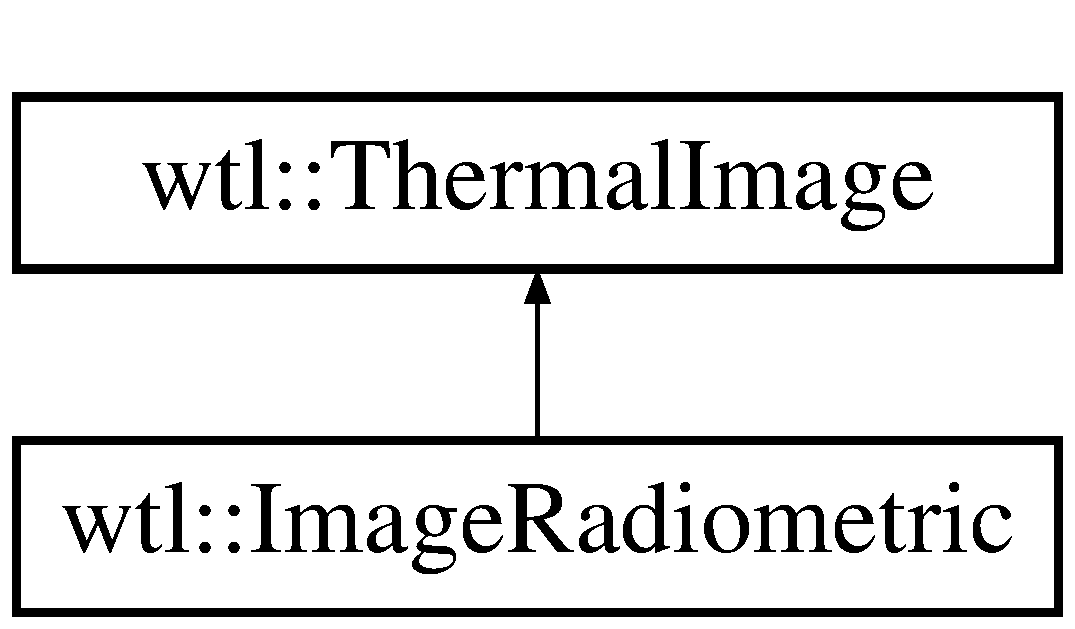
\includegraphics[height=2.000000cm]{classwtl_1_1_image_radiometric}
\end{center}
\end{figure}
\subsection*{Public Member Functions}
\begin{DoxyCompactItemize}
\item 
\hyperlink{classwtl_1_1_image_radiometric_a2d44ad864d81d556cd4909ad064a2809}{Image\+Radiometric} (const \hyperlink{classwtl_1_1_image_radiometric}{Image\+Radiometric} \&x)=delete
\item 
\hyperlink{classwtl_1_1_image_radiometric}{Image\+Radiometric} \& \hyperlink{classwtl_1_1_image_radiometric_aec1dfb43a074a912824fbf875e849040}{operator=} (const \hyperlink{classwtl_1_1_image_radiometric}{Image\+Radiometric} \&x)=delete
\item 
\hyperlink{classwtl_1_1_image_radiometric_ac82e2b4d611ef6c1386e18d1f91bb9dc}{$\sim$\+Image\+Radiometric} ()
\item 
uint16\+\_\+t \hyperlink{classwtl_1_1_image_radiometric_a54944b28818ee3d347f9b462744d0e49}{get\+Raw\+Radiometric\+Value} (int x, int y) const
\begin{DoxyCompactList}\small\item\em Get 16 bit radiometric value of an pixel. \end{DoxyCompactList}\item 
uint16\+\_\+t \hyperlink{classwtl_1_1_image_radiometric_a4e4591e2af9b3bc9d553bc991df68e2b}{get\+Signal} (int x, int y) const
\begin{DoxyCompactList}\small\item\em Get signal value of a pixel. \end{DoxyCompactList}\item 
float \hyperlink{classwtl_1_1_image_radiometric_aafdb4f226d077b561cf429d55451d9d1}{get\+Temperature} (int x, int y) const
\begin{DoxyCompactList}\small\item\em Get temperature of a pixel. \end{DoxyCompactList}\item 
float \hyperlink{classwtl_1_1_image_radiometric_a2d1922ffa3030f0344a7e1abf90a524d}{get\+Max\+Temperature} () const
\begin{DoxyCompactList}\small\item\em Get maximum temperature present in an image. \end{DoxyCompactList}\item 
std\+::pair$<$ int, int $>$ \hyperlink{classwtl_1_1_image_radiometric_ae1bdd0fb2335a6482ff3656dd8e9f7a3}{get\+Max\+Pos} () const
\begin{DoxyCompactList}\small\item\em Get position of pixel with maximux temperature. \end{DoxyCompactList}\item 
float \hyperlink{classwtl_1_1_image_radiometric_af615da6d48d04f430d8806edcd3fa61e}{get\+Min\+Temperature} () const
\begin{DoxyCompactList}\small\item\em Get minimum temperature present in an image. \end{DoxyCompactList}\item 
std\+::pair$<$ int, int $>$ \hyperlink{classwtl_1_1_image_radiometric_a4f8f918914c3de913e781de02c42e846}{get\+Min\+Pos} () const
\begin{DoxyCompactList}\small\item\em Get position of pixel with minimum temperature. \end{DoxyCompactList}\item 
float \hyperlink{classwtl_1_1_image_radiometric_afaa9e2ee77818d64c856f941ac3c26a3}{get\+Palette\+Max\+Temperature} () const
\begin{DoxyCompactList}\small\item\em \hyperlink{classwtl_1_1_image_radiometric_afaa9e2ee77818d64c856f941ac3c26a3}{wtl\+::\+Image\+Radiometric\+::get\+Palette\+Max\+Temperature} \end{DoxyCompactList}\item 
float \hyperlink{classwtl_1_1_image_radiometric_a8e604d89775064734e7d09bdf0ddb868}{get\+Palette\+Min\+Temperature} () const
\begin{DoxyCompactList}\small\item\em \hyperlink{classwtl_1_1_image_radiometric_a8e604d89775064734e7d09bdf0ddb868}{wtl\+::\+Image\+Radiometric\+::get\+Palette\+Min\+Temperature} \end{DoxyCompactList}\item 
const \hyperlink{structwtl_1_1_thermal_parameters}{Thermal\+Parameters} \& \hyperlink{classwtl_1_1_image_radiometric_a5d450d8ec4e2eed79b2481000290e6e0}{get\+Thermal\+Parameters} () const
\begin{DoxyCompactList}\small\item\em Get Thermal\+Parametres instance which contains all thermal parameters of an image. \end{DoxyCompactList}\item 
void \hyperlink{classwtl_1_1_image_radiometric_ab0f5b66e57cccb1b210e27e869a1e440}{get\+Temperature\+Array} (float $\ast$$\ast$image\+Data, int \&image\+Size) const
\begin{DoxyCompactList}\small\item\em Get array with temperatures from radiometric image. \end{DoxyCompactList}\item 
void \hyperlink{classwtl_1_1_image_radiometric_abf1750f399e3f48bff59e9e490f4139f}{get\+Signal\+Array} (uint16\+\_\+t $\ast$$\ast$image\+Data, int \&image\+Size) const
\begin{DoxyCompactList}\small\item\em Get array with signal values from radiometric image. \end{DoxyCompactList}\item 
void \hyperlink{classwtl_1_1_image_radiometric_a5d32b9f0e98f81d5e917e5d33625f254}{get\+Grayscale\+Array\+Representation} (uint8\+\_\+t $\ast$$\ast$image\+Data, int \&image\+Size) const
\begin{DoxyCompactList}\small\item\em Get array with grayscayscale representation of thermogram that can be directly used to visualize image. \end{DoxyCompactList}\item 
void \hyperlink{classwtl_1_1_image_radiometric_a53d894315e62d9a048b2888f9a63a023}{get\+R\+G\+B\+Array\+Representation} (uint8\+\_\+t $\ast$image\+Data, int \&image\+Size) const
\begin{DoxyCompactList}\small\item\em Get array with R\+GB representation of thermogram that can be directly used to visualize image. \end{DoxyCompactList}\item 
void \hyperlink{classwtl_1_1_image_radiometric_a27d9e4bcac88362a4957df7b10de83d8}{get\+R\+G\+B\+Array\+Representation} (uint8\+\_\+t $\ast$image\+Data, int \&image\+Size, std\+::vector$<$ int $>$ \&pixel\+Per\+Color\+Counter) const
\begin{DoxyCompactList}\small\item\em Get array with R\+GB representation of thermogram that can be directly used to visualize image. \end{DoxyCompactList}\item 
void \hyperlink{classwtl_1_1_image_radiometric_a98fd9036bc6d70aa5b09c50446862428}{get\+R\+G\+B\+Array\+Representation\+With\+Overlay} (uint8\+\_\+t $\ast$image\+Data, int \&image\+Size) const
\begin{DoxyCompactList}\small\item\em Get array with R\+GB representation of thermogram that can be directly used to visualize image. \hyperlink{classwtl_1_1_alarms}{Alarms} and measurements overlay is added to the image. \end{DoxyCompactList}\item 
void \hyperlink{classwtl_1_1_image_radiometric_a1d6f40074cec56b1149041b3782401fb}{get\+R\+G\+B\+Array\+Representation\+With\+Overlay} (uint8\+\_\+t $\ast$image\+Data, int \&image\+Size, std\+::vector$<$ int $>$ \&pixel\+Per\+Color\+Counter) const
\begin{DoxyCompactList}\small\item\em Get array with R\+GB representation of thermogram that can be directly used to visualize image. \hyperlink{classwtl_1_1_alarms}{Alarms} and measurements overlay is added to the image. \end{DoxyCompactList}\item 
void \hyperlink{classwtl_1_1_image_radiometric_a4f157b22b0b290f1d3c4ec2ddf0ed3b4}{get\+R\+G\+B\+Array\+Representation\+With\+Pal} (uint8\+\_\+t $\ast$$\ast$image\+Data, int \&image\+Size) const
\begin{DoxyCompactList}\small\item\em Get array with R\+GB representation of thermogram that can be directly used to visualize image. \end{DoxyCompactList}\item 
void \hyperlink{classwtl_1_1_image_radiometric_a0ebd547b95a0976e806bd55319127833}{recalculate\+Temperatures} ()
\begin{DoxyCompactList}\small\item\em Recalculate image temperatures. \end{DoxyCompactList}\item 
void \hyperlink{classwtl_1_1_image_radiometric_ab9e6959a9b90a234a8b7db6a7d283c97}{prepare\+Radiometric\+Data} ()
\begin{DoxyCompactList}\small\item\em Check for the rois that affect temperature measurement. \end{DoxyCompactList}\item 
bool \hyperlink{classwtl_1_1_image_radiometric_af8fdfed71f7374c52c1e6d9a50b0fa77}{is\+Super\+Res\+Image} ()
\begin{DoxyCompactList}\small\item\em Check whether image supports super-\/resolution. \end{DoxyCompactList}\item 
int \hyperlink{classwtl_1_1_image_radiometric_a8d52c493b7bd5c8568afa23734e025b0}{get\+Super\+Res\+Frame\+Count} ()
\begin{DoxyCompactList}\small\item\em Get number of frames captured in a image, superres image can have up to 60. \end{DoxyCompactList}\item 
uint16\+\_\+t $\ast$$\ast$ \hyperlink{classwtl_1_1_image_radiometric_a06ac3d38bbf4a8b705398c690fee7532}{get\+Pixels\+Super\+Res} (int $\ast$frames)
\begin{DoxyCompactList}\small\item\em Get pointer to pixel arrays of each frame. \end{DoxyCompactList}\item 
void \hyperlink{classwtl_1_1_image_radiometric_ac3064fb2a267f4b2a7975069e5da4920}{set\+Manual\+Max} (float value)
\begin{DoxyCompactList}\small\item\em Set temperature used as maximum for palette. \end{DoxyCompactList}\item 
void \hyperlink{classwtl_1_1_image_radiometric_ae700fe57e3bd44bb8f4ace0b85992fd9}{set\+Manual\+Min} (float value)
\begin{DoxyCompactList}\small\item\em Set temperature used as minimium for palette. \end{DoxyCompactList}\item 
void \hyperlink{classwtl_1_1_image_radiometric_af84a54aef49c990a1795aa20be584cae}{set\+Thermal\+Params} (const std\+::shared\+\_\+ptr$<$ \hyperlink{structwtl_1_1_thermal_parameters}{wtl\+::\+Thermal\+Parameters} $>$ \&new\+Params)
\begin{DoxyCompactList}\small\item\em Copy all thermal params from \hyperlink{structwtl_1_1_thermal_parameters}{Thermal\+Parameters} instance. \end{DoxyCompactList}\item 
void \hyperlink{classwtl_1_1_image_radiometric_ae831386c8e1970728cfe0fd978735078}{set\+Emissivity} (double value)
\begin{DoxyCompactList}\small\item\em Set emissivity of objects on an image. \end{DoxyCompactList}\item 
void \hyperlink{classwtl_1_1_image_radiometric_acade58f2c02c2a37fce92f2f085d28f8}{set\+Reflected\+Temp} (double value)
\begin{DoxyCompactList}\small\item\em Set Reflected Temperature of objects on an image. \end{DoxyCompactList}\item 
void \hyperlink{classwtl_1_1_image_radiometric_a76ca53e05d839b3bb17faf7a054469ad}{set\+Atm\+Temp} (double value)
\begin{DoxyCompactList}\small\item\em Set Atmospheric Temperature. \end{DoxyCompactList}\item 
void \hyperlink{classwtl_1_1_image_radiometric_a94a4ff1210b47b3952f5996f1de591da}{set\+Extern\+Optic\+Temp} (double value)
\begin{DoxyCompactList}\small\item\em Set External Optics Temperature. \end{DoxyCompactList}\item 
void \hyperlink{classwtl_1_1_image_radiometric_ad1e5e233f3df59dff8fef5c37f4d1dc1}{set\+Object\+Distance} (double value)
\begin{DoxyCompactList}\small\item\em Set distance to objects in scene. \end{DoxyCompactList}\item 
void \hyperlink{classwtl_1_1_image_radiometric_af7382abba74ae6803928d636d8cd4c5a}{set\+Extern\+Optic\+Trans} (double value)
\begin{DoxyCompactList}\small\item\em Set External Optics Transition. \end{DoxyCompactList}\item 
void \hyperlink{classwtl_1_1_image_radiometric_a721bc10f81a64770f5e7d406595d9d40}{set\+Humidity} (double value)
\begin{DoxyCompactList}\small\item\em Set humidity. \end{DoxyCompactList}\item 
std\+::shared\+\_\+ptr$<$ \hyperlink{classwtl_1_1_measurements}{Measurements} $>$ \hyperlink{classwtl_1_1_image_radiometric_a906c58c168250da7412d53626f34aba1}{get\+Measurements} () const
\begin{DoxyCompactList}\small\item\em Get \hyperlink{classwtl_1_1_measurements}{Measurements}. \end{DoxyCompactList}\item 
std\+::shared\+\_\+ptr$<$ \hyperlink{classwtl_1_1_alarms}{Alarms} $>$ \hyperlink{classwtl_1_1_image_radiometric_a6589459ee934ba5b857db30d359150b1}{get\+Alarms} () const
\begin{DoxyCompactList}\small\item\em Get \hyperlink{classwtl_1_1_alarms}{Alarms}. \end{DoxyCompactList}\item 
double \hyperlink{classwtl_1_1_image_radiometric_a061574091d97bb6b9b2509d3c1dd592b}{get\+Emissivity} ()
\begin{DoxyCompactList}\small\item\em get\+Emissivity. \end{DoxyCompactList}\item 
double \hyperlink{classwtl_1_1_image_radiometric_a32bbd3d1b9bbc4086218520bb1d5a16d}{get\+Reflected\+Temp} ()
\begin{DoxyCompactList}\small\item\em Reflected Temperature saved in an image. \end{DoxyCompactList}\item 
double \hyperlink{classwtl_1_1_image_radiometric_a4a41b730ce5d5dc31bf6f008398d0058}{get\+Atm\+Temp} ()
\begin{DoxyCompactList}\small\item\em Atmospheric temperatur saved in an image. \end{DoxyCompactList}\item 
double \hyperlink{classwtl_1_1_image_radiometric_abec2a0d47751710396b065cf75a411e9}{get\+Extern\+Optic\+Temp} ()
\begin{DoxyCompactList}\small\item\em External Optics Temperature saved in an image. \end{DoxyCompactList}\item 
double \hyperlink{classwtl_1_1_image_radiometric_a6286201924bb258db0c1a2a4396f6f50}{get\+Object\+Distance} ()
\begin{DoxyCompactList}\small\item\em Distance of an captured object on image. \end{DoxyCompactList}\item 
double \hyperlink{classwtl_1_1_image_radiometric_a314bfd568c6c7d2ed38ef599802939a2}{get\+Extern\+Optic\+Trans} ()
\begin{DoxyCompactList}\small\item\em External optics transmission saved in an image. \end{DoxyCompactList}\item 
double \hyperlink{classwtl_1_1_image_radiometric_a994da652e39fdf2f53cb3e3b8bc6e243}{get\+Humidity} ()
\begin{DoxyCompactList}\small\item\em Relative humidity saved in an image. \end{DoxyCompactList}\item 
bool \hyperlink{classwtl_1_1_image_radiometric_a0805bd9404ae42b94f9c47c52c19d4e6}{is\+Radiometric\+Image} () const
\begin{DoxyCompactList}\small\item\em Decide whether thermal image instance contains temperature data. \end{DoxyCompactList}\item 
void \hyperlink{classwtl_1_1_image_radiometric_ac430cfe342329fd5077a33abf1eefd71}{add\+Roi\+To\+Image} (std\+::shared\+\_\+ptr$<$ \hyperlink{structwtl_1_1_roi_struct}{Roi\+Struct} $>$ roi)
\begin{DoxyCompactList}\small\item\em Add R\+OI item to image. \end{DoxyCompactList}\item 
void \hyperlink{classwtl_1_1_image_radiometric_a8f6724db0c63140cadb237f053105c57}{remove\+Roi\+From\+Image} (std\+::shared\+\_\+ptr$<$ \hyperlink{structwtl_1_1_roi_struct}{Roi\+Struct} $>$ roi)
\begin{DoxyCompactList}\small\item\em Remove R\+OI item from image. \end{DoxyCompactList}\item 
void \hyperlink{classwtl_1_1_image_radiometric_ad7b4937dedd3d70c0be19b41940f3083}{add\+Roi\+To\+Image} (const \hyperlink{structwtl_1_1_roi_struct}{Roi\+Struct} \&roi)
\begin{DoxyCompactList}\small\item\em Add R\+OI item to image. \end{DoxyCompactList}\item 
void \hyperlink{classwtl_1_1_image_radiometric_aa9b47acd750ac06f7cd19601f6641ebc}{update\+Custom\+Params\+Roi} (\hyperlink{structwtl_1_1_roi_struct}{Roi\+Struct} \&roi, bool custom\+Params, float emissivity, float refl\+Temp, float distance)
\begin{DoxyCompactList}\small\item\em update\+Custom\+Params\+Roi \end{DoxyCompactList}\item 
void \hyperlink{classwtl_1_1_image_radiometric_ae9b9a7da380a4681826ab7d610f909d2}{add\+Alarm\+To\+Image} (std\+::shared\+\_\+ptr$<$ \hyperlink{structwtl_1_1_alarm_struct}{Alarm\+Struct} $>$ alarm)
\begin{DoxyCompactList}\small\item\em Add Alarm item to image. \end{DoxyCompactList}\item 
void \hyperlink{classwtl_1_1_image_radiometric_a3e7eb6b8c50f85dc43cc1e2f372cdd3f}{add\+Alarm\+To\+Image} (const \hyperlink{structwtl_1_1_alarm_struct}{Alarm\+Struct} \&alarm)
\begin{DoxyCompactList}\small\item\em Add Alarm item to image. \end{DoxyCompactList}\item 
bool \hyperlink{classwtl_1_1_image_radiometric_a5fb5c3570bf545a469c8e6cd210bb360}{recalc\+Roi} (std\+::shared\+\_\+ptr$<$ \hyperlink{structwtl_1_1_roi_struct}{Roi\+Struct} $>$ roi, float \&roi\+Max, std\+::pair$<$ int, int $>$ \&max\+Coords, float \&roi\+Min, std\+::pair$<$ int, int $>$ \&min\+Coords, float \&roi\+Avg)
\begin{DoxyCompactList}\small\item\em Recalculate temperatures inside roi item. \end{DoxyCompactList}\item 
bool \hyperlink{classwtl_1_1_image_radiometric_a7563fba10935fdf522f89e8a2b91688f}{recalc\+Roi} (\hyperlink{structwtl_1_1_roi_struct}{Roi\+Struct} \&roi, float \&roi\+Max, std\+::pair$<$ int, int $>$ \&max\+Coords, float \&roi\+Min, std\+::pair$<$ int, int $>$ \&min\+Coords, float \&roi\+Avg)
\begin{DoxyCompactList}\small\item\em Recalculate temperatures inside roi item. \end{DoxyCompactList}\end{DoxyCompactItemize}
\subsection*{Friends}
\begin{DoxyCompactItemize}
\item 
class \hyperlink{classwtl_1_1_image_radiometric_a5baf0a1f190dbaabf7033b4ba92f4c81}{Center}
\item 
class \hyperlink{classwtl_1_1_image_radiometric_a89f52b56f7155da8da3c26ad5feb1bcc}{F\+F\+F\+File\+Manager}
\item 
class \hyperlink{classwtl_1_1_image_radiometric_abb080e4a18ea68b1b97a42e193004b14}{Sequence\+Radiometric}
\end{DoxyCompactItemize}
\subsection*{Additional Inherited Members}


\subsection{Detailed Description}
Derived Class representing thermogram with temperature data and thermal parameters included. 

Provides interface for extracting and saving data to radiometric images. Instances are created only trough functions in class \hyperlink{classwtl_1_1_center}{Center}. A radiometric J\+P\+EG is a standard J\+P\+EG with a F\+F\+F-\/file inserted in the A\+P\+P1-\/tag 

\subsection{Constructor \& Destructor Documentation}
\mbox{\Hypertarget{classwtl_1_1_image_radiometric_a2d44ad864d81d556cd4909ad064a2809}\label{classwtl_1_1_image_radiometric_a2d44ad864d81d556cd4909ad064a2809}} 
\index{wtl\+::\+Image\+Radiometric@{wtl\+::\+Image\+Radiometric}!Image\+Radiometric@{Image\+Radiometric}}
\index{Image\+Radiometric@{Image\+Radiometric}!wtl\+::\+Image\+Radiometric@{wtl\+::\+Image\+Radiometric}}
\subsubsection{\texorpdfstring{Image\+Radiometric()}{ImageRadiometric()}}
{\footnotesize\ttfamily wtl\+::\+Image\+Radiometric\+::\+Image\+Radiometric (\begin{DoxyParamCaption}\item[{const \hyperlink{classwtl_1_1_image_radiometric}{Image\+Radiometric} \&}]{x }\end{DoxyParamCaption})\hspace{0.3cm}{\ttfamily [delete]}}

\mbox{\Hypertarget{classwtl_1_1_image_radiometric_ac82e2b4d611ef6c1386e18d1f91bb9dc}\label{classwtl_1_1_image_radiometric_ac82e2b4d611ef6c1386e18d1f91bb9dc}} 
\index{wtl\+::\+Image\+Radiometric@{wtl\+::\+Image\+Radiometric}!````~Image\+Radiometric@{$\sim$\+Image\+Radiometric}}
\index{````~Image\+Radiometric@{$\sim$\+Image\+Radiometric}!wtl\+::\+Image\+Radiometric@{wtl\+::\+Image\+Radiometric}}
\subsubsection{\texorpdfstring{$\sim$\+Image\+Radiometric()}{~ImageRadiometric()}}
{\footnotesize\ttfamily wtl\+::\+Image\+Radiometric\+::$\sim$\+Image\+Radiometric (\begin{DoxyParamCaption}{ }\end{DoxyParamCaption})}



\subsection{Member Function Documentation}
\mbox{\Hypertarget{classwtl_1_1_image_radiometric_ae9b9a7da380a4681826ab7d610f909d2}\label{classwtl_1_1_image_radiometric_ae9b9a7da380a4681826ab7d610f909d2}} 
\index{wtl\+::\+Image\+Radiometric@{wtl\+::\+Image\+Radiometric}!add\+Alarm\+To\+Image@{add\+Alarm\+To\+Image}}
\index{add\+Alarm\+To\+Image@{add\+Alarm\+To\+Image}!wtl\+::\+Image\+Radiometric@{wtl\+::\+Image\+Radiometric}}
\subsubsection{\texorpdfstring{add\+Alarm\+To\+Image()}{addAlarmToImage()}\hspace{0.1cm}{\footnotesize\ttfamily [1/2]}}
{\footnotesize\ttfamily void wtl\+::\+Image\+Radiometric\+::add\+Alarm\+To\+Image (\begin{DoxyParamCaption}\item[{std\+::shared\+\_\+ptr$<$ \hyperlink{structwtl_1_1_alarm_struct}{Alarm\+Struct} $>$}]{alarm }\end{DoxyParamCaption})}



Add Alarm item to image. 


\begin{DoxyParams}{Parameters}
{\em alarm} & Alarm item. \\
\hline
\end{DoxyParams}
\mbox{\Hypertarget{classwtl_1_1_image_radiometric_a3e7eb6b8c50f85dc43cc1e2f372cdd3f}\label{classwtl_1_1_image_radiometric_a3e7eb6b8c50f85dc43cc1e2f372cdd3f}} 
\index{wtl\+::\+Image\+Radiometric@{wtl\+::\+Image\+Radiometric}!add\+Alarm\+To\+Image@{add\+Alarm\+To\+Image}}
\index{add\+Alarm\+To\+Image@{add\+Alarm\+To\+Image}!wtl\+::\+Image\+Radiometric@{wtl\+::\+Image\+Radiometric}}
\subsubsection{\texorpdfstring{add\+Alarm\+To\+Image()}{addAlarmToImage()}\hspace{0.1cm}{\footnotesize\ttfamily [2/2]}}
{\footnotesize\ttfamily void wtl\+::\+Image\+Radiometric\+::add\+Alarm\+To\+Image (\begin{DoxyParamCaption}\item[{const \hyperlink{structwtl_1_1_alarm_struct}{Alarm\+Struct} \&}]{alarm }\end{DoxyParamCaption})}



Add Alarm item to image. 


\begin{DoxyParams}{Parameters}
{\em alarm} & Alarm item. \\
\hline
\end{DoxyParams}
\mbox{\Hypertarget{classwtl_1_1_image_radiometric_ac430cfe342329fd5077a33abf1eefd71}\label{classwtl_1_1_image_radiometric_ac430cfe342329fd5077a33abf1eefd71}} 
\index{wtl\+::\+Image\+Radiometric@{wtl\+::\+Image\+Radiometric}!add\+Roi\+To\+Image@{add\+Roi\+To\+Image}}
\index{add\+Roi\+To\+Image@{add\+Roi\+To\+Image}!wtl\+::\+Image\+Radiometric@{wtl\+::\+Image\+Radiometric}}
\subsubsection{\texorpdfstring{add\+Roi\+To\+Image()}{addRoiToImage()}\hspace{0.1cm}{\footnotesize\ttfamily [1/2]}}
{\footnotesize\ttfamily void wtl\+::\+Image\+Radiometric\+::add\+Roi\+To\+Image (\begin{DoxyParamCaption}\item[{std\+::shared\+\_\+ptr$<$ \hyperlink{structwtl_1_1_roi_struct}{Roi\+Struct} $>$}]{roi }\end{DoxyParamCaption})}



Add R\+OI item to image. 


\begin{DoxyParams}{Parameters}
{\em roi} & R\+OI item. \\
\hline
\end{DoxyParams}
\mbox{\Hypertarget{classwtl_1_1_image_radiometric_ad7b4937dedd3d70c0be19b41940f3083}\label{classwtl_1_1_image_radiometric_ad7b4937dedd3d70c0be19b41940f3083}} 
\index{wtl\+::\+Image\+Radiometric@{wtl\+::\+Image\+Radiometric}!add\+Roi\+To\+Image@{add\+Roi\+To\+Image}}
\index{add\+Roi\+To\+Image@{add\+Roi\+To\+Image}!wtl\+::\+Image\+Radiometric@{wtl\+::\+Image\+Radiometric}}
\subsubsection{\texorpdfstring{add\+Roi\+To\+Image()}{addRoiToImage()}\hspace{0.1cm}{\footnotesize\ttfamily [2/2]}}
{\footnotesize\ttfamily void wtl\+::\+Image\+Radiometric\+::add\+Roi\+To\+Image (\begin{DoxyParamCaption}\item[{const \hyperlink{structwtl_1_1_roi_struct}{Roi\+Struct} \&}]{roi }\end{DoxyParamCaption})}



Add R\+OI item to image. 


\begin{DoxyParams}{Parameters}
{\em roi} & R\+OI item. \\
\hline
\end{DoxyParams}
\mbox{\Hypertarget{classwtl_1_1_image_radiometric_a6589459ee934ba5b857db30d359150b1}\label{classwtl_1_1_image_radiometric_a6589459ee934ba5b857db30d359150b1}} 
\index{wtl\+::\+Image\+Radiometric@{wtl\+::\+Image\+Radiometric}!get\+Alarms@{get\+Alarms}}
\index{get\+Alarms@{get\+Alarms}!wtl\+::\+Image\+Radiometric@{wtl\+::\+Image\+Radiometric}}
\subsubsection{\texorpdfstring{get\+Alarms()}{getAlarms()}}
{\footnotesize\ttfamily std\+::shared\+\_\+ptr$<$ \hyperlink{classwtl_1_1_alarms}{wtl\+::\+Alarms} $>$ wtl\+::\+Image\+Radiometric\+::get\+Alarms (\begin{DoxyParamCaption}{ }\end{DoxyParamCaption}) const}



Get \hyperlink{classwtl_1_1_alarms}{Alarms}. 

\begin{DoxyReturn}{Returns}
Shared pointer to all the alarms present in a source 
\end{DoxyReturn}
\mbox{\Hypertarget{classwtl_1_1_image_radiometric_a4a41b730ce5d5dc31bf6f008398d0058}\label{classwtl_1_1_image_radiometric_a4a41b730ce5d5dc31bf6f008398d0058}} 
\index{wtl\+::\+Image\+Radiometric@{wtl\+::\+Image\+Radiometric}!get\+Atm\+Temp@{get\+Atm\+Temp}}
\index{get\+Atm\+Temp@{get\+Atm\+Temp}!wtl\+::\+Image\+Radiometric@{wtl\+::\+Image\+Radiometric}}
\subsubsection{\texorpdfstring{get\+Atm\+Temp()}{getAtmTemp()}}
{\footnotesize\ttfamily double wtl\+::\+Image\+Radiometric\+::get\+Atm\+Temp (\begin{DoxyParamCaption}{ }\end{DoxyParamCaption})}



Atmospheric temperatur saved in an image. 

\begin{DoxyReturn}{Returns}
Atmospheric temperature. 
\end{DoxyReturn}
\mbox{\Hypertarget{classwtl_1_1_image_radiometric_a061574091d97bb6b9b2509d3c1dd592b}\label{classwtl_1_1_image_radiometric_a061574091d97bb6b9b2509d3c1dd592b}} 
\index{wtl\+::\+Image\+Radiometric@{wtl\+::\+Image\+Radiometric}!get\+Emissivity@{get\+Emissivity}}
\index{get\+Emissivity@{get\+Emissivity}!wtl\+::\+Image\+Radiometric@{wtl\+::\+Image\+Radiometric}}
\subsubsection{\texorpdfstring{get\+Emissivity()}{getEmissivity()}}
{\footnotesize\ttfamily double wtl\+::\+Image\+Radiometric\+::get\+Emissivity (\begin{DoxyParamCaption}{ }\end{DoxyParamCaption})}



get\+Emissivity. 

\begin{DoxyReturn}{Returns}
Image emissivity. 
\end{DoxyReturn}
\mbox{\Hypertarget{classwtl_1_1_image_radiometric_abec2a0d47751710396b065cf75a411e9}\label{classwtl_1_1_image_radiometric_abec2a0d47751710396b065cf75a411e9}} 
\index{wtl\+::\+Image\+Radiometric@{wtl\+::\+Image\+Radiometric}!get\+Extern\+Optic\+Temp@{get\+Extern\+Optic\+Temp}}
\index{get\+Extern\+Optic\+Temp@{get\+Extern\+Optic\+Temp}!wtl\+::\+Image\+Radiometric@{wtl\+::\+Image\+Radiometric}}
\subsubsection{\texorpdfstring{get\+Extern\+Optic\+Temp()}{getExternOpticTemp()}}
{\footnotesize\ttfamily double wtl\+::\+Image\+Radiometric\+::get\+Extern\+Optic\+Temp (\begin{DoxyParamCaption}{ }\end{DoxyParamCaption})}



External Optics Temperature saved in an image. 

\begin{DoxyReturn}{Returns}
External Optics Temperature. 
\end{DoxyReturn}
\mbox{\Hypertarget{classwtl_1_1_image_radiometric_a314bfd568c6c7d2ed38ef599802939a2}\label{classwtl_1_1_image_radiometric_a314bfd568c6c7d2ed38ef599802939a2}} 
\index{wtl\+::\+Image\+Radiometric@{wtl\+::\+Image\+Radiometric}!get\+Extern\+Optic\+Trans@{get\+Extern\+Optic\+Trans}}
\index{get\+Extern\+Optic\+Trans@{get\+Extern\+Optic\+Trans}!wtl\+::\+Image\+Radiometric@{wtl\+::\+Image\+Radiometric}}
\subsubsection{\texorpdfstring{get\+Extern\+Optic\+Trans()}{getExternOpticTrans()}}
{\footnotesize\ttfamily double wtl\+::\+Image\+Radiometric\+::get\+Extern\+Optic\+Trans (\begin{DoxyParamCaption}{ }\end{DoxyParamCaption})}



External optics transmission saved in an image. 

\begin{DoxyReturn}{Returns}
External optics transmission. 
\end{DoxyReturn}
\mbox{\Hypertarget{classwtl_1_1_image_radiometric_a5d32b9f0e98f81d5e917e5d33625f254}\label{classwtl_1_1_image_radiometric_a5d32b9f0e98f81d5e917e5d33625f254}} 
\index{wtl\+::\+Image\+Radiometric@{wtl\+::\+Image\+Radiometric}!get\+Grayscale\+Array\+Representation@{get\+Grayscale\+Array\+Representation}}
\index{get\+Grayscale\+Array\+Representation@{get\+Grayscale\+Array\+Representation}!wtl\+::\+Image\+Radiometric@{wtl\+::\+Image\+Radiometric}}
\subsubsection{\texorpdfstring{get\+Grayscale\+Array\+Representation()}{getGrayscaleArrayRepresentation()}}
{\footnotesize\ttfamily void wtl\+::\+Image\+Radiometric\+::get\+Grayscale\+Array\+Representation (\begin{DoxyParamCaption}\item[{uint8\+\_\+t $\ast$$\ast$}]{image\+Data,  }\item[{int \&}]{image\+Size }\end{DoxyParamCaption}) const\hspace{0.3cm}{\ttfamily [virtual]}}



Get array with grayscayscale representation of thermogram that can be directly used to visualize image. 


\begin{DoxyParams}[1]{Parameters}
\mbox{\tt out}  & {\em image\+Data} & Output array parameter. \\
\hline
\mbox{\tt out}  & {\em image\+Size} & Size of an array. \\
\hline
\end{DoxyParams}


Implements \hyperlink{classwtl_1_1_thermal_image_ad43f8aa46870634ad5cdd5dd784046fc}{wtl\+::\+Thermal\+Image}.

\mbox{\Hypertarget{classwtl_1_1_image_radiometric_a994da652e39fdf2f53cb3e3b8bc6e243}\label{classwtl_1_1_image_radiometric_a994da652e39fdf2f53cb3e3b8bc6e243}} 
\index{wtl\+::\+Image\+Radiometric@{wtl\+::\+Image\+Radiometric}!get\+Humidity@{get\+Humidity}}
\index{get\+Humidity@{get\+Humidity}!wtl\+::\+Image\+Radiometric@{wtl\+::\+Image\+Radiometric}}
\subsubsection{\texorpdfstring{get\+Humidity()}{getHumidity()}}
{\footnotesize\ttfamily double wtl\+::\+Image\+Radiometric\+::get\+Humidity (\begin{DoxyParamCaption}{ }\end{DoxyParamCaption})}



Relative humidity saved in an image. 

\begin{DoxyReturn}{Returns}
Relative humidity. 
\end{DoxyReturn}
\mbox{\Hypertarget{classwtl_1_1_image_radiometric_ae1bdd0fb2335a6482ff3656dd8e9f7a3}\label{classwtl_1_1_image_radiometric_ae1bdd0fb2335a6482ff3656dd8e9f7a3}} 
\index{wtl\+::\+Image\+Radiometric@{wtl\+::\+Image\+Radiometric}!get\+Max\+Pos@{get\+Max\+Pos}}
\index{get\+Max\+Pos@{get\+Max\+Pos}!wtl\+::\+Image\+Radiometric@{wtl\+::\+Image\+Radiometric}}
\subsubsection{\texorpdfstring{get\+Max\+Pos()}{getMaxPos()}}
{\footnotesize\ttfamily std\+::pair$<$ int, int $>$ wtl\+::\+Image\+Radiometric\+::get\+Max\+Pos (\begin{DoxyParamCaption}{ }\end{DoxyParamCaption}) const\hspace{0.3cm}{\ttfamily [virtual]}}



Get position of pixel with maximux temperature. 

\begin{DoxyReturn}{Returns}
Coordinates of Maximum temperature captured in an image. 
\end{DoxyReturn}


Implements \hyperlink{classwtl_1_1_thermal_image_af5c649f864be43c3f0f4f9bacc047345}{wtl\+::\+Thermal\+Image}.

\mbox{\Hypertarget{classwtl_1_1_image_radiometric_a2d1922ffa3030f0344a7e1abf90a524d}\label{classwtl_1_1_image_radiometric_a2d1922ffa3030f0344a7e1abf90a524d}} 
\index{wtl\+::\+Image\+Radiometric@{wtl\+::\+Image\+Radiometric}!get\+Max\+Temperature@{get\+Max\+Temperature}}
\index{get\+Max\+Temperature@{get\+Max\+Temperature}!wtl\+::\+Image\+Radiometric@{wtl\+::\+Image\+Radiometric}}
\subsubsection{\texorpdfstring{get\+Max\+Temperature()}{getMaxTemperature()}}
{\footnotesize\ttfamily float wtl\+::\+Image\+Radiometric\+::get\+Max\+Temperature (\begin{DoxyParamCaption}{ }\end{DoxyParamCaption}) const}



Get maximum temperature present in an image. 

\begin{DoxyReturn}{Returns}
Maximum temperature captured in an image. 
\end{DoxyReturn}
\mbox{\Hypertarget{classwtl_1_1_image_radiometric_a906c58c168250da7412d53626f34aba1}\label{classwtl_1_1_image_radiometric_a906c58c168250da7412d53626f34aba1}} 
\index{wtl\+::\+Image\+Radiometric@{wtl\+::\+Image\+Radiometric}!get\+Measurements@{get\+Measurements}}
\index{get\+Measurements@{get\+Measurements}!wtl\+::\+Image\+Radiometric@{wtl\+::\+Image\+Radiometric}}
\subsubsection{\texorpdfstring{get\+Measurements()}{getMeasurements()}}
{\footnotesize\ttfamily std\+::shared\+\_\+ptr$<$ \hyperlink{classwtl_1_1_measurements}{wtl\+::\+Measurements} $>$ wtl\+::\+Image\+Radiometric\+::get\+Measurements (\begin{DoxyParamCaption}{ }\end{DoxyParamCaption}) const}



Get \hyperlink{classwtl_1_1_measurements}{Measurements}. 

\begin{DoxyReturn}{Returns}
Shared pointer to all the measurements present in a source 
\end{DoxyReturn}
\mbox{\Hypertarget{classwtl_1_1_image_radiometric_a4f8f918914c3de913e781de02c42e846}\label{classwtl_1_1_image_radiometric_a4f8f918914c3de913e781de02c42e846}} 
\index{wtl\+::\+Image\+Radiometric@{wtl\+::\+Image\+Radiometric}!get\+Min\+Pos@{get\+Min\+Pos}}
\index{get\+Min\+Pos@{get\+Min\+Pos}!wtl\+::\+Image\+Radiometric@{wtl\+::\+Image\+Radiometric}}
\subsubsection{\texorpdfstring{get\+Min\+Pos()}{getMinPos()}}
{\footnotesize\ttfamily std\+::pair$<$ int, int $>$ wtl\+::\+Image\+Radiometric\+::get\+Min\+Pos (\begin{DoxyParamCaption}{ }\end{DoxyParamCaption}) const\hspace{0.3cm}{\ttfamily [virtual]}}



Get position of pixel with minimum temperature. 

\begin{DoxyReturn}{Returns}
Coordinates of point with minimal temperature captured in an image. 
\end{DoxyReturn}


Implements \hyperlink{classwtl_1_1_thermal_image_a9887878b3965566660ce4c434873603a}{wtl\+::\+Thermal\+Image}.

\mbox{\Hypertarget{classwtl_1_1_image_radiometric_af615da6d48d04f430d8806edcd3fa61e}\label{classwtl_1_1_image_radiometric_af615da6d48d04f430d8806edcd3fa61e}} 
\index{wtl\+::\+Image\+Radiometric@{wtl\+::\+Image\+Radiometric}!get\+Min\+Temperature@{get\+Min\+Temperature}}
\index{get\+Min\+Temperature@{get\+Min\+Temperature}!wtl\+::\+Image\+Radiometric@{wtl\+::\+Image\+Radiometric}}
\subsubsection{\texorpdfstring{get\+Min\+Temperature()}{getMinTemperature()}}
{\footnotesize\ttfamily float wtl\+::\+Image\+Radiometric\+::get\+Min\+Temperature (\begin{DoxyParamCaption}{ }\end{DoxyParamCaption}) const}



Get minimum temperature present in an image. 

\begin{DoxyReturn}{Returns}
Minimm temperature captured in an image. 
\end{DoxyReturn}
\mbox{\Hypertarget{classwtl_1_1_image_radiometric_a6286201924bb258db0c1a2a4396f6f50}\label{classwtl_1_1_image_radiometric_a6286201924bb258db0c1a2a4396f6f50}} 
\index{wtl\+::\+Image\+Radiometric@{wtl\+::\+Image\+Radiometric}!get\+Object\+Distance@{get\+Object\+Distance}}
\index{get\+Object\+Distance@{get\+Object\+Distance}!wtl\+::\+Image\+Radiometric@{wtl\+::\+Image\+Radiometric}}
\subsubsection{\texorpdfstring{get\+Object\+Distance()}{getObjectDistance()}}
{\footnotesize\ttfamily double wtl\+::\+Image\+Radiometric\+::get\+Object\+Distance (\begin{DoxyParamCaption}{ }\end{DoxyParamCaption})}



Distance of an captured object on image. 

\begin{DoxyReturn}{Returns}
Distance of an captured object. 
\end{DoxyReturn}
\mbox{\Hypertarget{classwtl_1_1_image_radiometric_afaa9e2ee77818d64c856f941ac3c26a3}\label{classwtl_1_1_image_radiometric_afaa9e2ee77818d64c856f941ac3c26a3}} 
\index{wtl\+::\+Image\+Radiometric@{wtl\+::\+Image\+Radiometric}!get\+Palette\+Max\+Temperature@{get\+Palette\+Max\+Temperature}}
\index{get\+Palette\+Max\+Temperature@{get\+Palette\+Max\+Temperature}!wtl\+::\+Image\+Radiometric@{wtl\+::\+Image\+Radiometric}}
\subsubsection{\texorpdfstring{get\+Palette\+Max\+Temperature()}{getPaletteMaxTemperature()}}
{\footnotesize\ttfamily float wtl\+::\+Image\+Radiometric\+::get\+Palette\+Max\+Temperature (\begin{DoxyParamCaption}{ }\end{DoxyParamCaption}) const}



\hyperlink{classwtl_1_1_image_radiometric_afaa9e2ee77818d64c856f941ac3c26a3}{wtl\+::\+Image\+Radiometric\+::get\+Palette\+Max\+Temperature} 

\begin{DoxyReturn}{Returns}

\end{DoxyReturn}
\mbox{\Hypertarget{classwtl_1_1_image_radiometric_a8e604d89775064734e7d09bdf0ddb868}\label{classwtl_1_1_image_radiometric_a8e604d89775064734e7d09bdf0ddb868}} 
\index{wtl\+::\+Image\+Radiometric@{wtl\+::\+Image\+Radiometric}!get\+Palette\+Min\+Temperature@{get\+Palette\+Min\+Temperature}}
\index{get\+Palette\+Min\+Temperature@{get\+Palette\+Min\+Temperature}!wtl\+::\+Image\+Radiometric@{wtl\+::\+Image\+Radiometric}}
\subsubsection{\texorpdfstring{get\+Palette\+Min\+Temperature()}{getPaletteMinTemperature()}}
{\footnotesize\ttfamily float wtl\+::\+Image\+Radiometric\+::get\+Palette\+Min\+Temperature (\begin{DoxyParamCaption}{ }\end{DoxyParamCaption}) const}



\hyperlink{classwtl_1_1_image_radiometric_a8e604d89775064734e7d09bdf0ddb868}{wtl\+::\+Image\+Radiometric\+::get\+Palette\+Min\+Temperature} 

\begin{DoxyReturn}{Returns}

\end{DoxyReturn}
\mbox{\Hypertarget{classwtl_1_1_image_radiometric_a06ac3d38bbf4a8b705398c690fee7532}\label{classwtl_1_1_image_radiometric_a06ac3d38bbf4a8b705398c690fee7532}} 
\index{wtl\+::\+Image\+Radiometric@{wtl\+::\+Image\+Radiometric}!get\+Pixels\+Super\+Res@{get\+Pixels\+Super\+Res}}
\index{get\+Pixels\+Super\+Res@{get\+Pixels\+Super\+Res}!wtl\+::\+Image\+Radiometric@{wtl\+::\+Image\+Radiometric}}
\subsubsection{\texorpdfstring{get\+Pixels\+Super\+Res()}{getPixelsSuperRes()}}
{\footnotesize\ttfamily uint16\+\_\+t $\ast$$\ast$ wtl\+::\+Image\+Radiometric\+::get\+Pixels\+Super\+Res (\begin{DoxyParamCaption}\item[{int $\ast$}]{frames }\end{DoxyParamCaption})}



Get pointer to pixel arrays of each frame. 


\begin{DoxyParams}{Parameters}
{\em frames} & \\
\hline
\end{DoxyParams}
\begin{DoxyReturn}{Returns}

\end{DoxyReturn}
\mbox{\Hypertarget{classwtl_1_1_image_radiometric_a54944b28818ee3d347f9b462744d0e49}\label{classwtl_1_1_image_radiometric_a54944b28818ee3d347f9b462744d0e49}} 
\index{wtl\+::\+Image\+Radiometric@{wtl\+::\+Image\+Radiometric}!get\+Raw\+Radiometric\+Value@{get\+Raw\+Radiometric\+Value}}
\index{get\+Raw\+Radiometric\+Value@{get\+Raw\+Radiometric\+Value}!wtl\+::\+Image\+Radiometric@{wtl\+::\+Image\+Radiometric}}
\subsubsection{\texorpdfstring{get\+Raw\+Radiometric\+Value()}{getRawRadiometricValue()}}
{\footnotesize\ttfamily uint16\+\_\+t wtl\+::\+Image\+Radiometric\+::get\+Raw\+Radiometric\+Value (\begin{DoxyParamCaption}\item[{int}]{x,  }\item[{int}]{y }\end{DoxyParamCaption}) const}



Get 16 bit radiometric value of an pixel. 

Radiometric value in linearized and is simply convertible to Kelvins. 
\begin{DoxyParams}{Parameters}
{\em x} & Width coordinate. \\
\hline
{\em y} & Height coordinate. \\
\hline
\end{DoxyParams}
\begin{DoxyReturn}{Returns}
16 bit Radiometric value at given pixel. 
\end{DoxyReturn}
\mbox{\Hypertarget{classwtl_1_1_image_radiometric_a32bbd3d1b9bbc4086218520bb1d5a16d}\label{classwtl_1_1_image_radiometric_a32bbd3d1b9bbc4086218520bb1d5a16d}} 
\index{wtl\+::\+Image\+Radiometric@{wtl\+::\+Image\+Radiometric}!get\+Reflected\+Temp@{get\+Reflected\+Temp}}
\index{get\+Reflected\+Temp@{get\+Reflected\+Temp}!wtl\+::\+Image\+Radiometric@{wtl\+::\+Image\+Radiometric}}
\subsubsection{\texorpdfstring{get\+Reflected\+Temp()}{getReflectedTemp()}}
{\footnotesize\ttfamily double wtl\+::\+Image\+Radiometric\+::get\+Reflected\+Temp (\begin{DoxyParamCaption}{ }\end{DoxyParamCaption})}



Reflected Temperature saved in an image. 

\begin{DoxyReturn}{Returns}
Reflected Temperature. 
\end{DoxyReturn}
\mbox{\Hypertarget{classwtl_1_1_image_radiometric_a53d894315e62d9a048b2888f9a63a023}\label{classwtl_1_1_image_radiometric_a53d894315e62d9a048b2888f9a63a023}} 
\index{wtl\+::\+Image\+Radiometric@{wtl\+::\+Image\+Radiometric}!get\+R\+G\+B\+Array\+Representation@{get\+R\+G\+B\+Array\+Representation}}
\index{get\+R\+G\+B\+Array\+Representation@{get\+R\+G\+B\+Array\+Representation}!wtl\+::\+Image\+Radiometric@{wtl\+::\+Image\+Radiometric}}
\subsubsection{\texorpdfstring{get\+R\+G\+B\+Array\+Representation()}{getRGBArrayRepresentation()}\hspace{0.1cm}{\footnotesize\ttfamily [1/2]}}
{\footnotesize\ttfamily void wtl\+::\+Image\+Radiometric\+::get\+R\+G\+B\+Array\+Representation (\begin{DoxyParamCaption}\item[{uint8\+\_\+t $\ast$}]{image\+Data,  }\item[{int \&}]{image\+Size }\end{DoxyParamCaption}) const\hspace{0.3cm}{\ttfamily [virtual]}}



Get array with R\+GB representation of thermogram that can be directly used to visualize image. 


\begin{DoxyParams}[1]{Parameters}
\mbox{\tt out}  & {\em image\+Data} & Output array parameter. \\
\hline
\mbox{\tt out}  & {\em image\+Size} & Size of an array. \\
\hline
\end{DoxyParams}


Implements \hyperlink{classwtl_1_1_thermal_image_ae19943330497206817cda3557c4a0725}{wtl\+::\+Thermal\+Image}.

\mbox{\Hypertarget{classwtl_1_1_image_radiometric_a27d9e4bcac88362a4957df7b10de83d8}\label{classwtl_1_1_image_radiometric_a27d9e4bcac88362a4957df7b10de83d8}} 
\index{wtl\+::\+Image\+Radiometric@{wtl\+::\+Image\+Radiometric}!get\+R\+G\+B\+Array\+Representation@{get\+R\+G\+B\+Array\+Representation}}
\index{get\+R\+G\+B\+Array\+Representation@{get\+R\+G\+B\+Array\+Representation}!wtl\+::\+Image\+Radiometric@{wtl\+::\+Image\+Radiometric}}
\subsubsection{\texorpdfstring{get\+R\+G\+B\+Array\+Representation()}{getRGBArrayRepresentation()}\hspace{0.1cm}{\footnotesize\ttfamily [2/2]}}
{\footnotesize\ttfamily void wtl\+::\+Image\+Radiometric\+::get\+R\+G\+B\+Array\+Representation (\begin{DoxyParamCaption}\item[{uint8\+\_\+t $\ast$}]{image\+Data,  }\item[{int \&}]{image\+Size,  }\item[{std\+::vector$<$ int $>$ \&}]{pixel\+Per\+Color\+Counter }\end{DoxyParamCaption}) const}



Get array with R\+GB representation of thermogram that can be directly used to visualize image. 


\begin{DoxyParams}[1]{Parameters}
\mbox{\tt out}  & {\em image\+Data} & Output array parameter. \\
\hline
\mbox{\tt out}  & {\em image\+Size} & Size of an array. \\
\hline
\mbox{\tt out}  & {\em pixel\+Per\+Color\+Counter} & vector that has number of pixels of color i at index i. \\
\hline
\end{DoxyParams}
\mbox{\Hypertarget{classwtl_1_1_image_radiometric_a98fd9036bc6d70aa5b09c50446862428}\label{classwtl_1_1_image_radiometric_a98fd9036bc6d70aa5b09c50446862428}} 
\index{wtl\+::\+Image\+Radiometric@{wtl\+::\+Image\+Radiometric}!get\+R\+G\+B\+Array\+Representation\+With\+Overlay@{get\+R\+G\+B\+Array\+Representation\+With\+Overlay}}
\index{get\+R\+G\+B\+Array\+Representation\+With\+Overlay@{get\+R\+G\+B\+Array\+Representation\+With\+Overlay}!wtl\+::\+Image\+Radiometric@{wtl\+::\+Image\+Radiometric}}
\subsubsection{\texorpdfstring{get\+R\+G\+B\+Array\+Representation\+With\+Overlay()}{getRGBArrayRepresentationWithOverlay()}\hspace{0.1cm}{\footnotesize\ttfamily [1/2]}}
{\footnotesize\ttfamily void wtl\+::\+Image\+Radiometric\+::get\+R\+G\+B\+Array\+Representation\+With\+Overlay (\begin{DoxyParamCaption}\item[{uint8\+\_\+t $\ast$}]{image\+Data,  }\item[{int \&}]{image\+Size }\end{DoxyParamCaption}) const\hspace{0.3cm}{\ttfamily [virtual]}}



Get array with R\+GB representation of thermogram that can be directly used to visualize image. \hyperlink{classwtl_1_1_alarms}{Alarms} and measurements overlay is added to the image. 


\begin{DoxyParams}[1]{Parameters}
\mbox{\tt out}  & {\em image\+Data} & Output array parameter. \\
\hline
\mbox{\tt out}  & {\em image\+Size} & Size of an array. \\
\hline
\end{DoxyParams}


Implements \hyperlink{classwtl_1_1_thermal_image_a02a4771bd8c9e571d195fe86b7b856f2}{wtl\+::\+Thermal\+Image}.

\mbox{\Hypertarget{classwtl_1_1_image_radiometric_a1d6f40074cec56b1149041b3782401fb}\label{classwtl_1_1_image_radiometric_a1d6f40074cec56b1149041b3782401fb}} 
\index{wtl\+::\+Image\+Radiometric@{wtl\+::\+Image\+Radiometric}!get\+R\+G\+B\+Array\+Representation\+With\+Overlay@{get\+R\+G\+B\+Array\+Representation\+With\+Overlay}}
\index{get\+R\+G\+B\+Array\+Representation\+With\+Overlay@{get\+R\+G\+B\+Array\+Representation\+With\+Overlay}!wtl\+::\+Image\+Radiometric@{wtl\+::\+Image\+Radiometric}}
\subsubsection{\texorpdfstring{get\+R\+G\+B\+Array\+Representation\+With\+Overlay()}{getRGBArrayRepresentationWithOverlay()}\hspace{0.1cm}{\footnotesize\ttfamily [2/2]}}
{\footnotesize\ttfamily void wtl\+::\+Image\+Radiometric\+::get\+R\+G\+B\+Array\+Representation\+With\+Overlay (\begin{DoxyParamCaption}\item[{uint8\+\_\+t $\ast$}]{image\+Data,  }\item[{int \&}]{image\+Size,  }\item[{std\+::vector$<$ int $>$ \&}]{pixel\+Per\+Color\+Counter }\end{DoxyParamCaption}) const}



Get array with R\+GB representation of thermogram that can be directly used to visualize image. \hyperlink{classwtl_1_1_alarms}{Alarms} and measurements overlay is added to the image. 


\begin{DoxyParams}[1]{Parameters}
\mbox{\tt out}  & {\em image\+Data} & Output array parameter. \\
\hline
\mbox{\tt out}  & {\em image\+Size} & Size of an array. \\
\hline
\mbox{\tt out}  & {\em pixel\+Per\+Color\+Counter} & vector that has number of pixels of color i at index i. \\
\hline
\end{DoxyParams}
\mbox{\Hypertarget{classwtl_1_1_image_radiometric_a4f157b22b0b290f1d3c4ec2ddf0ed3b4}\label{classwtl_1_1_image_radiometric_a4f157b22b0b290f1d3c4ec2ddf0ed3b4}} 
\index{wtl\+::\+Image\+Radiometric@{wtl\+::\+Image\+Radiometric}!get\+R\+G\+B\+Array\+Representation\+With\+Pal@{get\+R\+G\+B\+Array\+Representation\+With\+Pal}}
\index{get\+R\+G\+B\+Array\+Representation\+With\+Pal@{get\+R\+G\+B\+Array\+Representation\+With\+Pal}!wtl\+::\+Image\+Radiometric@{wtl\+::\+Image\+Radiometric}}
\subsubsection{\texorpdfstring{get\+R\+G\+B\+Array\+Representation\+With\+Pal()}{getRGBArrayRepresentationWithPal()}}
{\footnotesize\ttfamily void wtl\+::\+Image\+Radiometric\+::get\+R\+G\+B\+Array\+Representation\+With\+Pal (\begin{DoxyParamCaption}\item[{uint8\+\_\+t $\ast$$\ast$}]{image\+Data,  }\item[{int \&}]{image\+Size }\end{DoxyParamCaption}) const}



Get array with R\+GB representation of thermogram that can be directly used to visualize image. 

Includes palette miniature. 
\begin{DoxyParams}[1]{Parameters}
\mbox{\tt out}  & {\em image\+Data} & Output array parameter. \\
\hline
\mbox{\tt out}  & {\em image\+Size} & Size of an array. \\
\hline
\end{DoxyParams}
\mbox{\Hypertarget{classwtl_1_1_image_radiometric_a4e4591e2af9b3bc9d553bc991df68e2b}\label{classwtl_1_1_image_radiometric_a4e4591e2af9b3bc9d553bc991df68e2b}} 
\index{wtl\+::\+Image\+Radiometric@{wtl\+::\+Image\+Radiometric}!get\+Signal@{get\+Signal}}
\index{get\+Signal@{get\+Signal}!wtl\+::\+Image\+Radiometric@{wtl\+::\+Image\+Radiometric}}
\subsubsection{\texorpdfstring{get\+Signal()}{getSignal()}}
{\footnotesize\ttfamily uint16\+\_\+t wtl\+::\+Image\+Radiometric\+::get\+Signal (\begin{DoxyParamCaption}\item[{int}]{x,  }\item[{int}]{y }\end{DoxyParamCaption}) const}



Get signal value of a pixel. 


\begin{DoxyParams}{Parameters}
{\em x} & Width coordinate. \\
\hline
{\em y} & Height coordinate. \\
\hline
\end{DoxyParams}
\begin{DoxyReturn}{Returns}
Signal value at given pixel. 
\end{DoxyReturn}
\mbox{\Hypertarget{classwtl_1_1_image_radiometric_abf1750f399e3f48bff59e9e490f4139f}\label{classwtl_1_1_image_radiometric_abf1750f399e3f48bff59e9e490f4139f}} 
\index{wtl\+::\+Image\+Radiometric@{wtl\+::\+Image\+Radiometric}!get\+Signal\+Array@{get\+Signal\+Array}}
\index{get\+Signal\+Array@{get\+Signal\+Array}!wtl\+::\+Image\+Radiometric@{wtl\+::\+Image\+Radiometric}}
\subsubsection{\texorpdfstring{get\+Signal\+Array()}{getSignalArray()}}
{\footnotesize\ttfamily void wtl\+::\+Image\+Radiometric\+::get\+Signal\+Array (\begin{DoxyParamCaption}\item[{uint16\+\_\+t $\ast$$\ast$}]{image\+Data,  }\item[{int \&}]{image\+Size }\end{DoxyParamCaption}) const}



Get array with signal values from radiometric image. 


\begin{DoxyParams}[1]{Parameters}
\mbox{\tt out}  & {\em image\+Data} & Output array parameter. \\
\hline
\mbox{\tt out}  & {\em image\+Size} & Size of an array. \\
\hline
\end{DoxyParams}
\mbox{\Hypertarget{classwtl_1_1_image_radiometric_a8d52c493b7bd5c8568afa23734e025b0}\label{classwtl_1_1_image_radiometric_a8d52c493b7bd5c8568afa23734e025b0}} 
\index{wtl\+::\+Image\+Radiometric@{wtl\+::\+Image\+Radiometric}!get\+Super\+Res\+Frame\+Count@{get\+Super\+Res\+Frame\+Count}}
\index{get\+Super\+Res\+Frame\+Count@{get\+Super\+Res\+Frame\+Count}!wtl\+::\+Image\+Radiometric@{wtl\+::\+Image\+Radiometric}}
\subsubsection{\texorpdfstring{get\+Super\+Res\+Frame\+Count()}{getSuperResFrameCount()}}
{\footnotesize\ttfamily int wtl\+::\+Image\+Radiometric\+::get\+Super\+Res\+Frame\+Count (\begin{DoxyParamCaption}{ }\end{DoxyParamCaption})}



Get number of frames captured in a image, superres image can have up to 60. 

\begin{DoxyReturn}{Returns}

\end{DoxyReturn}
\mbox{\Hypertarget{classwtl_1_1_image_radiometric_aafdb4f226d077b561cf429d55451d9d1}\label{classwtl_1_1_image_radiometric_aafdb4f226d077b561cf429d55451d9d1}} 
\index{wtl\+::\+Image\+Radiometric@{wtl\+::\+Image\+Radiometric}!get\+Temperature@{get\+Temperature}}
\index{get\+Temperature@{get\+Temperature}!wtl\+::\+Image\+Radiometric@{wtl\+::\+Image\+Radiometric}}
\subsubsection{\texorpdfstring{get\+Temperature()}{getTemperature()}}
{\footnotesize\ttfamily float wtl\+::\+Image\+Radiometric\+::get\+Temperature (\begin{DoxyParamCaption}\item[{int}]{x,  }\item[{int}]{y }\end{DoxyParamCaption}) const}



Get temperature of a pixel. 


\begin{DoxyParams}{Parameters}
{\em x} & Width coordinate. \\
\hline
{\em y} & Height coordinate. \\
\hline
\end{DoxyParams}
\begin{DoxyReturn}{Returns}
Temperature at given pixel. 
\end{DoxyReturn}
\mbox{\Hypertarget{classwtl_1_1_image_radiometric_ab0f5b66e57cccb1b210e27e869a1e440}\label{classwtl_1_1_image_radiometric_ab0f5b66e57cccb1b210e27e869a1e440}} 
\index{wtl\+::\+Image\+Radiometric@{wtl\+::\+Image\+Radiometric}!get\+Temperature\+Array@{get\+Temperature\+Array}}
\index{get\+Temperature\+Array@{get\+Temperature\+Array}!wtl\+::\+Image\+Radiometric@{wtl\+::\+Image\+Radiometric}}
\subsubsection{\texorpdfstring{get\+Temperature\+Array()}{getTemperatureArray()}}
{\footnotesize\ttfamily void wtl\+::\+Image\+Radiometric\+::get\+Temperature\+Array (\begin{DoxyParamCaption}\item[{float $\ast$$\ast$}]{image\+Data,  }\item[{int \&}]{image\+Size }\end{DoxyParamCaption}) const}



Get array with temperatures from radiometric image. 


\begin{DoxyParams}[1]{Parameters}
\mbox{\tt out}  & {\em image\+Data} & Output array parameter. \\
\hline
\mbox{\tt out}  & {\em image\+Size} & Size of an array. \\
\hline
\end{DoxyParams}
\mbox{\Hypertarget{classwtl_1_1_image_radiometric_a5d450d8ec4e2eed79b2481000290e6e0}\label{classwtl_1_1_image_radiometric_a5d450d8ec4e2eed79b2481000290e6e0}} 
\index{wtl\+::\+Image\+Radiometric@{wtl\+::\+Image\+Radiometric}!get\+Thermal\+Parameters@{get\+Thermal\+Parameters}}
\index{get\+Thermal\+Parameters@{get\+Thermal\+Parameters}!wtl\+::\+Image\+Radiometric@{wtl\+::\+Image\+Radiometric}}
\subsubsection{\texorpdfstring{get\+Thermal\+Parameters()}{getThermalParameters()}}
{\footnotesize\ttfamily const \hyperlink{structwtl_1_1_thermal_parameters}{wtl\+::\+Thermal\+Parameters} \& wtl\+::\+Image\+Radiometric\+::get\+Thermal\+Parameters (\begin{DoxyParamCaption}{ }\end{DoxyParamCaption}) const}



Get Thermal\+Parametres instance which contains all thermal parameters of an image. 

\begin{DoxyReturn}{Returns}
Instance can be used to access sequence meta data such as resolution, location, date of capture etc. 
\end{DoxyReturn}
\mbox{\Hypertarget{classwtl_1_1_image_radiometric_a0805bd9404ae42b94f9c47c52c19d4e6}\label{classwtl_1_1_image_radiometric_a0805bd9404ae42b94f9c47c52c19d4e6}} 
\index{wtl\+::\+Image\+Radiometric@{wtl\+::\+Image\+Radiometric}!is\+Radiometric\+Image@{is\+Radiometric\+Image}}
\index{is\+Radiometric\+Image@{is\+Radiometric\+Image}!wtl\+::\+Image\+Radiometric@{wtl\+::\+Image\+Radiometric}}
\subsubsection{\texorpdfstring{is\+Radiometric\+Image()}{isRadiometricImage()}}
{\footnotesize\ttfamily bool wtl\+::\+Image\+Radiometric\+::is\+Radiometric\+Image (\begin{DoxyParamCaption}{ }\end{DoxyParamCaption}) const\hspace{0.3cm}{\ttfamily [virtual]}}



Decide whether thermal image instance contains temperature data. 

\begin{DoxyReturn}{Returns}
True if image contains temperature for every pixel. 
\end{DoxyReturn}


Implements \hyperlink{classwtl_1_1_thermal_image_a6414e809f033c1813ac6801afcfb84b5}{wtl\+::\+Thermal\+Image}.

\mbox{\Hypertarget{classwtl_1_1_image_radiometric_af8fdfed71f7374c52c1e6d9a50b0fa77}\label{classwtl_1_1_image_radiometric_af8fdfed71f7374c52c1e6d9a50b0fa77}} 
\index{wtl\+::\+Image\+Radiometric@{wtl\+::\+Image\+Radiometric}!is\+Super\+Res\+Image@{is\+Super\+Res\+Image}}
\index{is\+Super\+Res\+Image@{is\+Super\+Res\+Image}!wtl\+::\+Image\+Radiometric@{wtl\+::\+Image\+Radiometric}}
\subsubsection{\texorpdfstring{is\+Super\+Res\+Image()}{isSuperResImage()}}
{\footnotesize\ttfamily bool wtl\+::\+Image\+Radiometric\+::is\+Super\+Res\+Image (\begin{DoxyParamCaption}{ }\end{DoxyParamCaption})}



Check whether image supports super-\/resolution. 

Superresolution algorithm enhances image resolution from multipla frames captured in and image. \begin{DoxyReturn}{Returns}
True if supperresolution is available. 
\end{DoxyReturn}
\mbox{\Hypertarget{classwtl_1_1_image_radiometric_aec1dfb43a074a912824fbf875e849040}\label{classwtl_1_1_image_radiometric_aec1dfb43a074a912824fbf875e849040}} 
\index{wtl\+::\+Image\+Radiometric@{wtl\+::\+Image\+Radiometric}!operator=@{operator=}}
\index{operator=@{operator=}!wtl\+::\+Image\+Radiometric@{wtl\+::\+Image\+Radiometric}}
\subsubsection{\texorpdfstring{operator=()}{operator=()}}
{\footnotesize\ttfamily \hyperlink{classwtl_1_1_image_radiometric}{Image\+Radiometric}\& wtl\+::\+Image\+Radiometric\+::operator= (\begin{DoxyParamCaption}\item[{const \hyperlink{classwtl_1_1_image_radiometric}{Image\+Radiometric} \&}]{x }\end{DoxyParamCaption})\hspace{0.3cm}{\ttfamily [delete]}}

\mbox{\Hypertarget{classwtl_1_1_image_radiometric_ab9e6959a9b90a234a8b7db6a7d283c97}\label{classwtl_1_1_image_radiometric_ab9e6959a9b90a234a8b7db6a7d283c97}} 
\index{wtl\+::\+Image\+Radiometric@{wtl\+::\+Image\+Radiometric}!prepare\+Radiometric\+Data@{prepare\+Radiometric\+Data}}
\index{prepare\+Radiometric\+Data@{prepare\+Radiometric\+Data}!wtl\+::\+Image\+Radiometric@{wtl\+::\+Image\+Radiometric}}
\subsubsection{\texorpdfstring{prepare\+Radiometric\+Data()}{prepareRadiometricData()}}
{\footnotesize\ttfamily void wtl\+::\+Image\+Radiometric\+::prepare\+Radiometric\+Data (\begin{DoxyParamCaption}{ }\end{DoxyParamCaption})}



Check for the rois that affect temperature measurement. 

\mbox{\Hypertarget{classwtl_1_1_image_radiometric_a5fb5c3570bf545a469c8e6cd210bb360}\label{classwtl_1_1_image_radiometric_a5fb5c3570bf545a469c8e6cd210bb360}} 
\index{wtl\+::\+Image\+Radiometric@{wtl\+::\+Image\+Radiometric}!recalc\+Roi@{recalc\+Roi}}
\index{recalc\+Roi@{recalc\+Roi}!wtl\+::\+Image\+Radiometric@{wtl\+::\+Image\+Radiometric}}
\subsubsection{\texorpdfstring{recalc\+Roi()}{recalcRoi()}\hspace{0.1cm}{\footnotesize\ttfamily [1/2]}}
{\footnotesize\ttfamily bool wtl\+::\+Image\+Radiometric\+::recalc\+Roi (\begin{DoxyParamCaption}\item[{std\+::shared\+\_\+ptr$<$ \hyperlink{structwtl_1_1_roi_struct}{Roi\+Struct} $>$}]{roi,  }\item[{float \&}]{roi\+Max,  }\item[{std\+::pair$<$ int, int $>$ \&}]{max\+Coords,  }\item[{float \&}]{roi\+Min,  }\item[{std\+::pair$<$ int, int $>$ \&}]{min\+Coords,  }\item[{float \&}]{roi\+Avg }\end{DoxyParamCaption})}



Recalculate temperatures inside roi item. 

\mbox{\Hypertarget{classwtl_1_1_image_radiometric_a7563fba10935fdf522f89e8a2b91688f}\label{classwtl_1_1_image_radiometric_a7563fba10935fdf522f89e8a2b91688f}} 
\index{wtl\+::\+Image\+Radiometric@{wtl\+::\+Image\+Radiometric}!recalc\+Roi@{recalc\+Roi}}
\index{recalc\+Roi@{recalc\+Roi}!wtl\+::\+Image\+Radiometric@{wtl\+::\+Image\+Radiometric}}
\subsubsection{\texorpdfstring{recalc\+Roi()}{recalcRoi()}\hspace{0.1cm}{\footnotesize\ttfamily [2/2]}}
{\footnotesize\ttfamily bool wtl\+::\+Image\+Radiometric\+::recalc\+Roi (\begin{DoxyParamCaption}\item[{\hyperlink{structwtl_1_1_roi_struct}{Roi\+Struct} \&}]{roi,  }\item[{float \&}]{roi\+Max,  }\item[{std\+::pair$<$ int, int $>$ \&}]{max\+Coords,  }\item[{float \&}]{roi\+Min,  }\item[{std\+::pair$<$ int, int $>$ \&}]{min\+Coords,  }\item[{float \&}]{roi\+Avg }\end{DoxyParamCaption})}



Recalculate temperatures inside roi item. 

\mbox{\Hypertarget{classwtl_1_1_image_radiometric_a0ebd547b95a0976e806bd55319127833}\label{classwtl_1_1_image_radiometric_a0ebd547b95a0976e806bd55319127833}} 
\index{wtl\+::\+Image\+Radiometric@{wtl\+::\+Image\+Radiometric}!recalculate\+Temperatures@{recalculate\+Temperatures}}
\index{recalculate\+Temperatures@{recalculate\+Temperatures}!wtl\+::\+Image\+Radiometric@{wtl\+::\+Image\+Radiometric}}
\subsubsection{\texorpdfstring{recalculate\+Temperatures()}{recalculateTemperatures()}}
{\footnotesize\ttfamily void wtl\+::\+Image\+Radiometric\+::recalculate\+Temperatures (\begin{DoxyParamCaption}{ }\end{DoxyParamCaption})}



Recalculate image temperatures. 

\mbox{\Hypertarget{classwtl_1_1_image_radiometric_a8f6724db0c63140cadb237f053105c57}\label{classwtl_1_1_image_radiometric_a8f6724db0c63140cadb237f053105c57}} 
\index{wtl\+::\+Image\+Radiometric@{wtl\+::\+Image\+Radiometric}!remove\+Roi\+From\+Image@{remove\+Roi\+From\+Image}}
\index{remove\+Roi\+From\+Image@{remove\+Roi\+From\+Image}!wtl\+::\+Image\+Radiometric@{wtl\+::\+Image\+Radiometric}}
\subsubsection{\texorpdfstring{remove\+Roi\+From\+Image()}{removeRoiFromImage()}}
{\footnotesize\ttfamily void wtl\+::\+Image\+Radiometric\+::remove\+Roi\+From\+Image (\begin{DoxyParamCaption}\item[{std\+::shared\+\_\+ptr$<$ \hyperlink{structwtl_1_1_roi_struct}{Roi\+Struct} $>$}]{roi }\end{DoxyParamCaption})}



Remove R\+OI item from image. 


\begin{DoxyParams}{Parameters}
{\em roi} & R\+OI item. \\
\hline
\end{DoxyParams}
\mbox{\Hypertarget{classwtl_1_1_image_radiometric_a76ca53e05d839b3bb17faf7a054469ad}\label{classwtl_1_1_image_radiometric_a76ca53e05d839b3bb17faf7a054469ad}} 
\index{wtl\+::\+Image\+Radiometric@{wtl\+::\+Image\+Radiometric}!set\+Atm\+Temp@{set\+Atm\+Temp}}
\index{set\+Atm\+Temp@{set\+Atm\+Temp}!wtl\+::\+Image\+Radiometric@{wtl\+::\+Image\+Radiometric}}
\subsubsection{\texorpdfstring{set\+Atm\+Temp()}{setAtmTemp()}}
{\footnotesize\ttfamily void wtl\+::\+Image\+Radiometric\+::set\+Atm\+Temp (\begin{DoxyParamCaption}\item[{double}]{value }\end{DoxyParamCaption})}



Set Atmospheric Temperature. 


\begin{DoxyParams}{Parameters}
{\em value} & New Atmospheric temperature value. \\
\hline
\end{DoxyParams}
\mbox{\Hypertarget{classwtl_1_1_image_radiometric_ae831386c8e1970728cfe0fd978735078}\label{classwtl_1_1_image_radiometric_ae831386c8e1970728cfe0fd978735078}} 
\index{wtl\+::\+Image\+Radiometric@{wtl\+::\+Image\+Radiometric}!set\+Emissivity@{set\+Emissivity}}
\index{set\+Emissivity@{set\+Emissivity}!wtl\+::\+Image\+Radiometric@{wtl\+::\+Image\+Radiometric}}
\subsubsection{\texorpdfstring{set\+Emissivity()}{setEmissivity()}}
{\footnotesize\ttfamily void wtl\+::\+Image\+Radiometric\+::set\+Emissivity (\begin{DoxyParamCaption}\item[{double}]{value }\end{DoxyParamCaption})}



Set emissivity of objects on an image. 


\begin{DoxyParams}{Parameters}
{\em value} & New emissivity value. \\
\hline
\end{DoxyParams}
\mbox{\Hypertarget{classwtl_1_1_image_radiometric_a94a4ff1210b47b3952f5996f1de591da}\label{classwtl_1_1_image_radiometric_a94a4ff1210b47b3952f5996f1de591da}} 
\index{wtl\+::\+Image\+Radiometric@{wtl\+::\+Image\+Radiometric}!set\+Extern\+Optic\+Temp@{set\+Extern\+Optic\+Temp}}
\index{set\+Extern\+Optic\+Temp@{set\+Extern\+Optic\+Temp}!wtl\+::\+Image\+Radiometric@{wtl\+::\+Image\+Radiometric}}
\subsubsection{\texorpdfstring{set\+Extern\+Optic\+Temp()}{setExternOpticTemp()}}
{\footnotesize\ttfamily void wtl\+::\+Image\+Radiometric\+::set\+Extern\+Optic\+Temp (\begin{DoxyParamCaption}\item[{double}]{value }\end{DoxyParamCaption})}



Set External Optics Temperature. 


\begin{DoxyParams}{Parameters}
{\em value} & New value. \\
\hline
\end{DoxyParams}
\mbox{\Hypertarget{classwtl_1_1_image_radiometric_af7382abba74ae6803928d636d8cd4c5a}\label{classwtl_1_1_image_radiometric_af7382abba74ae6803928d636d8cd4c5a}} 
\index{wtl\+::\+Image\+Radiometric@{wtl\+::\+Image\+Radiometric}!set\+Extern\+Optic\+Trans@{set\+Extern\+Optic\+Trans}}
\index{set\+Extern\+Optic\+Trans@{set\+Extern\+Optic\+Trans}!wtl\+::\+Image\+Radiometric@{wtl\+::\+Image\+Radiometric}}
\subsubsection{\texorpdfstring{set\+Extern\+Optic\+Trans()}{setExternOpticTrans()}}
{\footnotesize\ttfamily void wtl\+::\+Image\+Radiometric\+::set\+Extern\+Optic\+Trans (\begin{DoxyParamCaption}\item[{double}]{value }\end{DoxyParamCaption})}



Set External Optics Transition. 


\begin{DoxyParams}{Parameters}
{\em value} & New value. \\
\hline
\end{DoxyParams}
\mbox{\Hypertarget{classwtl_1_1_image_radiometric_a721bc10f81a64770f5e7d406595d9d40}\label{classwtl_1_1_image_radiometric_a721bc10f81a64770f5e7d406595d9d40}} 
\index{wtl\+::\+Image\+Radiometric@{wtl\+::\+Image\+Radiometric}!set\+Humidity@{set\+Humidity}}
\index{set\+Humidity@{set\+Humidity}!wtl\+::\+Image\+Radiometric@{wtl\+::\+Image\+Radiometric}}
\subsubsection{\texorpdfstring{set\+Humidity()}{setHumidity()}}
{\footnotesize\ttfamily void wtl\+::\+Image\+Radiometric\+::set\+Humidity (\begin{DoxyParamCaption}\item[{double}]{value }\end{DoxyParamCaption})}



Set humidity. 


\begin{DoxyParams}{Parameters}
{\em value} & New value. \\
\hline
\end{DoxyParams}
\mbox{\Hypertarget{classwtl_1_1_image_radiometric_ac3064fb2a267f4b2a7975069e5da4920}\label{classwtl_1_1_image_radiometric_ac3064fb2a267f4b2a7975069e5da4920}} 
\index{wtl\+::\+Image\+Radiometric@{wtl\+::\+Image\+Radiometric}!set\+Manual\+Max@{set\+Manual\+Max}}
\index{set\+Manual\+Max@{set\+Manual\+Max}!wtl\+::\+Image\+Radiometric@{wtl\+::\+Image\+Radiometric}}
\subsubsection{\texorpdfstring{set\+Manual\+Max()}{setManualMax()}}
{\footnotesize\ttfamily void wtl\+::\+Image\+Radiometric\+::set\+Manual\+Max (\begin{DoxyParamCaption}\item[{float}]{value }\end{DoxyParamCaption})}



Set temperature used as maximum for palette. 


\begin{DoxyParams}{Parameters}
{\em value} & Temperature in Celsius. \\
\hline
\end{DoxyParams}
\mbox{\Hypertarget{classwtl_1_1_image_radiometric_ae700fe57e3bd44bb8f4ace0b85992fd9}\label{classwtl_1_1_image_radiometric_ae700fe57e3bd44bb8f4ace0b85992fd9}} 
\index{wtl\+::\+Image\+Radiometric@{wtl\+::\+Image\+Radiometric}!set\+Manual\+Min@{set\+Manual\+Min}}
\index{set\+Manual\+Min@{set\+Manual\+Min}!wtl\+::\+Image\+Radiometric@{wtl\+::\+Image\+Radiometric}}
\subsubsection{\texorpdfstring{set\+Manual\+Min()}{setManualMin()}}
{\footnotesize\ttfamily void wtl\+::\+Image\+Radiometric\+::set\+Manual\+Min (\begin{DoxyParamCaption}\item[{float}]{value }\end{DoxyParamCaption})}



Set temperature used as minimium for palette. 


\begin{DoxyParams}{Parameters}
{\em value} & Temperature in Celsius. \\
\hline
\end{DoxyParams}
\mbox{\Hypertarget{classwtl_1_1_image_radiometric_ad1e5e233f3df59dff8fef5c37f4d1dc1}\label{classwtl_1_1_image_radiometric_ad1e5e233f3df59dff8fef5c37f4d1dc1}} 
\index{wtl\+::\+Image\+Radiometric@{wtl\+::\+Image\+Radiometric}!set\+Object\+Distance@{set\+Object\+Distance}}
\index{set\+Object\+Distance@{set\+Object\+Distance}!wtl\+::\+Image\+Radiometric@{wtl\+::\+Image\+Radiometric}}
\subsubsection{\texorpdfstring{set\+Object\+Distance()}{setObjectDistance()}}
{\footnotesize\ttfamily void wtl\+::\+Image\+Radiometric\+::set\+Object\+Distance (\begin{DoxyParamCaption}\item[{double}]{value }\end{DoxyParamCaption})}



Set distance to objects in scene. 


\begin{DoxyParams}{Parameters}
{\em value} & New value. \\
\hline
\end{DoxyParams}
\mbox{\Hypertarget{classwtl_1_1_image_radiometric_acade58f2c02c2a37fce92f2f085d28f8}\label{classwtl_1_1_image_radiometric_acade58f2c02c2a37fce92f2f085d28f8}} 
\index{wtl\+::\+Image\+Radiometric@{wtl\+::\+Image\+Radiometric}!set\+Reflected\+Temp@{set\+Reflected\+Temp}}
\index{set\+Reflected\+Temp@{set\+Reflected\+Temp}!wtl\+::\+Image\+Radiometric@{wtl\+::\+Image\+Radiometric}}
\subsubsection{\texorpdfstring{set\+Reflected\+Temp()}{setReflectedTemp()}}
{\footnotesize\ttfamily void wtl\+::\+Image\+Radiometric\+::set\+Reflected\+Temp (\begin{DoxyParamCaption}\item[{double}]{value }\end{DoxyParamCaption})}



Set Reflected Temperature of objects on an image. 


\begin{DoxyParams}{Parameters}
{\em value} & New Reflected\+Temp value. \\
\hline
\end{DoxyParams}
\mbox{\Hypertarget{classwtl_1_1_image_radiometric_af84a54aef49c990a1795aa20be584cae}\label{classwtl_1_1_image_radiometric_af84a54aef49c990a1795aa20be584cae}} 
\index{wtl\+::\+Image\+Radiometric@{wtl\+::\+Image\+Radiometric}!set\+Thermal\+Params@{set\+Thermal\+Params}}
\index{set\+Thermal\+Params@{set\+Thermal\+Params}!wtl\+::\+Image\+Radiometric@{wtl\+::\+Image\+Radiometric}}
\subsubsection{\texorpdfstring{set\+Thermal\+Params()}{setThermalParams()}}
{\footnotesize\ttfamily void wtl\+::\+Image\+Radiometric\+::set\+Thermal\+Params (\begin{DoxyParamCaption}\item[{const std\+::shared\+\_\+ptr$<$ \hyperlink{structwtl_1_1_thermal_parameters}{wtl\+::\+Thermal\+Parameters} $>$ \&}]{new\+Params }\end{DoxyParamCaption})}



Copy all thermal params from \hyperlink{structwtl_1_1_thermal_parameters}{Thermal\+Parameters} instance. 


\begin{DoxyParams}{Parameters}
{\em new\+Params} & \\
\hline
\end{DoxyParams}
\mbox{\Hypertarget{classwtl_1_1_image_radiometric_aa9b47acd750ac06f7cd19601f6641ebc}\label{classwtl_1_1_image_radiometric_aa9b47acd750ac06f7cd19601f6641ebc}} 
\index{wtl\+::\+Image\+Radiometric@{wtl\+::\+Image\+Radiometric}!update\+Custom\+Params\+Roi@{update\+Custom\+Params\+Roi}}
\index{update\+Custom\+Params\+Roi@{update\+Custom\+Params\+Roi}!wtl\+::\+Image\+Radiometric@{wtl\+::\+Image\+Radiometric}}
\subsubsection{\texorpdfstring{update\+Custom\+Params\+Roi()}{updateCustomParamsRoi()}}
{\footnotesize\ttfamily void wtl\+::\+Image\+Radiometric\+::update\+Custom\+Params\+Roi (\begin{DoxyParamCaption}\item[{\hyperlink{structwtl_1_1_roi_struct}{Roi\+Struct} \&}]{roi,  }\item[{bool}]{custom\+Params,  }\item[{float}]{emissivity,  }\item[{float}]{refl\+Temp,  }\item[{float}]{distance }\end{DoxyParamCaption})}



update\+Custom\+Params\+Roi 


\begin{DoxyParams}{Parameters}
{\em roi} & \\
\hline
{\em custom\+Params} & \\
\hline
{\em emissivity} & \\
\hline
{\em refl\+Temp} & \\
\hline
{\em distance} & \\
\hline
\end{DoxyParams}


\subsection{Friends And Related Function Documentation}
\mbox{\Hypertarget{classwtl_1_1_image_radiometric_a5baf0a1f190dbaabf7033b4ba92f4c81}\label{classwtl_1_1_image_radiometric_a5baf0a1f190dbaabf7033b4ba92f4c81}} 
\index{wtl\+::\+Image\+Radiometric@{wtl\+::\+Image\+Radiometric}!Center@{Center}}
\index{Center@{Center}!wtl\+::\+Image\+Radiometric@{wtl\+::\+Image\+Radiometric}}
\subsubsection{\texorpdfstring{Center}{Center}}
{\footnotesize\ttfamily friend class \hyperlink{classwtl_1_1_center}{Center}\hspace{0.3cm}{\ttfamily [friend]}}

\mbox{\Hypertarget{classwtl_1_1_image_radiometric_a89f52b56f7155da8da3c26ad5feb1bcc}\label{classwtl_1_1_image_radiometric_a89f52b56f7155da8da3c26ad5feb1bcc}} 
\index{wtl\+::\+Image\+Radiometric@{wtl\+::\+Image\+Radiometric}!F\+F\+F\+File\+Manager@{F\+F\+F\+File\+Manager}}
\index{F\+F\+F\+File\+Manager@{F\+F\+F\+File\+Manager}!wtl\+::\+Image\+Radiometric@{wtl\+::\+Image\+Radiometric}}
\subsubsection{\texorpdfstring{F\+F\+F\+File\+Manager}{FFFFileManager}}
{\footnotesize\ttfamily friend class F\+F\+F\+File\+Manager\hspace{0.3cm}{\ttfamily [friend]}}

\mbox{\Hypertarget{classwtl_1_1_image_radiometric_abb080e4a18ea68b1b97a42e193004b14}\label{classwtl_1_1_image_radiometric_abb080e4a18ea68b1b97a42e193004b14}} 
\index{wtl\+::\+Image\+Radiometric@{wtl\+::\+Image\+Radiometric}!Sequence\+Radiometric@{Sequence\+Radiometric}}
\index{Sequence\+Radiometric@{Sequence\+Radiometric}!wtl\+::\+Image\+Radiometric@{wtl\+::\+Image\+Radiometric}}
\subsubsection{\texorpdfstring{Sequence\+Radiometric}{SequenceRadiometric}}
{\footnotesize\ttfamily friend class \hyperlink{classwtl_1_1_sequence_radiometric}{Sequence\+Radiometric}\hspace{0.3cm}{\ttfamily [friend]}}


\hypertarget{classwtl_1_1_measurements}{}\section{wtl\+:\+:Measurements Class Reference}
\label{classwtl_1_1_measurements}\index{wtl\+::\+Measurements@{wtl\+::\+Measurements}}


Containter of all the measurements present in an image.  


\subsection*{Public Member Functions}
\begin{DoxyCompactItemize}
\item 
\hyperlink{classwtl_1_1_measurements_acb3ccc3f9a1a8322f80a8ff7891fec07}{Measurements} ()=default
\begin{DoxyCompactList}\small\item\em Default class constructor. \end{DoxyCompactList}\item 
\hyperlink{classwtl_1_1_measurements_a01e5d71f0613863ff9b156a7f420880a}{Measurements} (const \hyperlink{classwtl_1_1_measurements}{Measurements} \&x)=delete
\begin{DoxyCompactList}\small\item\em Deleted copy contructor. \end{DoxyCompactList}\item 
void \hyperlink{classwtl_1_1_measurements_a0e01de8663026fb293a904635f234745}{add\+Roi} (std\+::shared\+\_\+ptr$<$ \hyperlink{structwtl_1_1_roi_struct}{Roi\+Struct} $>$ roi)
\begin{DoxyCompactList}\small\item\em Add new Roi to the image. \end{DoxyCompactList}\item 
void \hyperlink{classwtl_1_1_measurements_ab0ea1cd53b62e0f86ad27761208832a6}{add\+Roi} (const \hyperlink{structwtl_1_1_roi_struct}{Roi\+Struct} \&roi)
\begin{DoxyCompactList}\small\item\em Add new Roi to the image. \end{DoxyCompactList}\item 
std\+::vector$<$ std\+::shared\+\_\+ptr$<$ \hyperlink{structwtl_1_1_roi_struct}{Roi\+Struct} $>$ $>$ \hyperlink{classwtl_1_1_measurements_a3e618f3c6ab36634fb4c01106a89b3fd}{get\+Rois} () const
\begin{DoxyCompactList}\small\item\em Get all the rois currently saved to the image. \end{DoxyCompactList}\item 
int \hyperlink{classwtl_1_1_measurements_a5f5e6c3dfecd34dbb6aad44f64abf2af}{get\+Roi\+Count} () const
\begin{DoxyCompactList}\small\item\em Roi Count. \end{DoxyCompactList}\item 
const \hyperlink{structwtl_1_1_roi_struct}{Roi\+Struct} \& \hyperlink{classwtl_1_1_measurements_a7120cb85575385e966f0a3af99814a47}{get\+Roi\+At} (int idx) const
\begin{DoxyCompactList}\small\item\em Get Roi by index. \end{DoxyCompactList}\item 
std\+::shared\+\_\+ptr$<$ \hyperlink{structwtl_1_1_roi_struct}{wtl\+::\+Roi\+Struct} $>$ \hyperlink{classwtl_1_1_measurements_ae12d47e8833b6d390d35473ade7be332}{get\+Roi\+Ptr\+At} (int idx) const
\begin{DoxyCompactList}\small\item\em Get Roi by index. \end{DoxyCompactList}\item 
bool \hyperlink{classwtl_1_1_measurements_a7f2320fef6dc9959686054a4bea6f77e}{delete\+Roi\+At} (int idx)
\begin{DoxyCompactList}\small\item\em Delete roi specified by index. \end{DoxyCompactList}\item 
bool \hyperlink{classwtl_1_1_measurements_a7fc7bb55f5b62b18736edd1470660b5e}{delete\+Roi\+From\+List} (std\+::shared\+\_\+ptr$<$ \hyperlink{structwtl_1_1_roi_struct}{Roi\+Struct} $>$ roi)
\begin{DoxyCompactList}\small\item\em Delete roi given by pointer from list. \end{DoxyCompactList}\item 
void \hyperlink{classwtl_1_1_measurements_abc23cb0e4c6b6dbae6637dad635171f9}{clear} ()
\begin{DoxyCompactList}\small\item\em clear all the measurements. \end{DoxyCompactList}\end{DoxyCompactItemize}


\subsection{Detailed Description}
Containter of all the measurements present in an image. 

Provides interface for reading saved measurements as well as adding new measurements. 

\subsection{Constructor \& Destructor Documentation}
\mbox{\Hypertarget{classwtl_1_1_measurements_acb3ccc3f9a1a8322f80a8ff7891fec07}\label{classwtl_1_1_measurements_acb3ccc3f9a1a8322f80a8ff7891fec07}} 
\index{wtl\+::\+Measurements@{wtl\+::\+Measurements}!Measurements@{Measurements}}
\index{Measurements@{Measurements}!wtl\+::\+Measurements@{wtl\+::\+Measurements}}
\subsubsection{\texorpdfstring{Measurements()}{Measurements()}\hspace{0.1cm}{\footnotesize\ttfamily [1/2]}}
{\footnotesize\ttfamily wtl\+::\+Measurements\+::\+Measurements (\begin{DoxyParamCaption}{ }\end{DoxyParamCaption})\hspace{0.3cm}{\ttfamily [default]}}



Default class constructor. 

\mbox{\Hypertarget{classwtl_1_1_measurements_a01e5d71f0613863ff9b156a7f420880a}\label{classwtl_1_1_measurements_a01e5d71f0613863ff9b156a7f420880a}} 
\index{wtl\+::\+Measurements@{wtl\+::\+Measurements}!Measurements@{Measurements}}
\index{Measurements@{Measurements}!wtl\+::\+Measurements@{wtl\+::\+Measurements}}
\subsubsection{\texorpdfstring{Measurements()}{Measurements()}\hspace{0.1cm}{\footnotesize\ttfamily [2/2]}}
{\footnotesize\ttfamily wtl\+::\+Measurements\+::\+Measurements (\begin{DoxyParamCaption}\item[{const \hyperlink{classwtl_1_1_measurements}{Measurements} \&}]{x }\end{DoxyParamCaption})\hspace{0.3cm}{\ttfamily [delete]}}



Deleted copy contructor. 



\subsection{Member Function Documentation}
\mbox{\Hypertarget{classwtl_1_1_measurements_a0e01de8663026fb293a904635f234745}\label{classwtl_1_1_measurements_a0e01de8663026fb293a904635f234745}} 
\index{wtl\+::\+Measurements@{wtl\+::\+Measurements}!add\+Roi@{add\+Roi}}
\index{add\+Roi@{add\+Roi}!wtl\+::\+Measurements@{wtl\+::\+Measurements}}
\subsubsection{\texorpdfstring{add\+Roi()}{addRoi()}\hspace{0.1cm}{\footnotesize\ttfamily [1/2]}}
{\footnotesize\ttfamily void wtl\+::\+Measurements\+::add\+Roi (\begin{DoxyParamCaption}\item[{std\+::shared\+\_\+ptr$<$ \hyperlink{structwtl_1_1_roi_struct}{Roi\+Struct} $>$}]{roi }\end{DoxyParamCaption})}



Add new Roi to the image. 


\begin{DoxyParams}{Parameters}
{\em roi} & Roi structure that is to be added. \\
\hline
\end{DoxyParams}
\mbox{\Hypertarget{classwtl_1_1_measurements_ab0ea1cd53b62e0f86ad27761208832a6}\label{classwtl_1_1_measurements_ab0ea1cd53b62e0f86ad27761208832a6}} 
\index{wtl\+::\+Measurements@{wtl\+::\+Measurements}!add\+Roi@{add\+Roi}}
\index{add\+Roi@{add\+Roi}!wtl\+::\+Measurements@{wtl\+::\+Measurements}}
\subsubsection{\texorpdfstring{add\+Roi()}{addRoi()}\hspace{0.1cm}{\footnotesize\ttfamily [2/2]}}
{\footnotesize\ttfamily void wtl\+::\+Measurements\+::add\+Roi (\begin{DoxyParamCaption}\item[{const \hyperlink{structwtl_1_1_roi_struct}{Roi\+Struct} \&}]{roi }\end{DoxyParamCaption})}



Add new Roi to the image. 


\begin{DoxyParams}{Parameters}
{\em roi} & Roi structure that is to be added. \\
\hline
\end{DoxyParams}
\mbox{\Hypertarget{classwtl_1_1_measurements_abc23cb0e4c6b6dbae6637dad635171f9}\label{classwtl_1_1_measurements_abc23cb0e4c6b6dbae6637dad635171f9}} 
\index{wtl\+::\+Measurements@{wtl\+::\+Measurements}!clear@{clear}}
\index{clear@{clear}!wtl\+::\+Measurements@{wtl\+::\+Measurements}}
\subsubsection{\texorpdfstring{clear()}{clear()}}
{\footnotesize\ttfamily void wtl\+::\+Measurements\+::clear (\begin{DoxyParamCaption}{ }\end{DoxyParamCaption})}



clear all the measurements. 

\mbox{\Hypertarget{classwtl_1_1_measurements_a7f2320fef6dc9959686054a4bea6f77e}\label{classwtl_1_1_measurements_a7f2320fef6dc9959686054a4bea6f77e}} 
\index{wtl\+::\+Measurements@{wtl\+::\+Measurements}!delete\+Roi\+At@{delete\+Roi\+At}}
\index{delete\+Roi\+At@{delete\+Roi\+At}!wtl\+::\+Measurements@{wtl\+::\+Measurements}}
\subsubsection{\texorpdfstring{delete\+Roi\+At()}{deleteRoiAt()}}
{\footnotesize\ttfamily bool wtl\+::\+Measurements\+::delete\+Roi\+At (\begin{DoxyParamCaption}\item[{int}]{idx }\end{DoxyParamCaption})}



Delete roi specified by index. 


\begin{DoxyParams}{Parameters}
{\em idx} & Roi index \\
\hline
\end{DoxyParams}
\begin{DoxyReturn}{Returns}

\end{DoxyReturn}
\mbox{\Hypertarget{classwtl_1_1_measurements_a7fc7bb55f5b62b18736edd1470660b5e}\label{classwtl_1_1_measurements_a7fc7bb55f5b62b18736edd1470660b5e}} 
\index{wtl\+::\+Measurements@{wtl\+::\+Measurements}!delete\+Roi\+From\+List@{delete\+Roi\+From\+List}}
\index{delete\+Roi\+From\+List@{delete\+Roi\+From\+List}!wtl\+::\+Measurements@{wtl\+::\+Measurements}}
\subsubsection{\texorpdfstring{delete\+Roi\+From\+List()}{deleteRoiFromList()}}
{\footnotesize\ttfamily bool wtl\+::\+Measurements\+::delete\+Roi\+From\+List (\begin{DoxyParamCaption}\item[{std\+::shared\+\_\+ptr$<$ \hyperlink{structwtl_1_1_roi_struct}{Roi\+Struct} $>$}]{roi }\end{DoxyParamCaption})}



Delete roi given by pointer from list. 


\begin{DoxyParams}{Parameters}
{\em roi} & Instance to be deleted from the list \\
\hline
\end{DoxyParams}
\begin{DoxyReturn}{Returns}

\end{DoxyReturn}
\mbox{\Hypertarget{classwtl_1_1_measurements_a7120cb85575385e966f0a3af99814a47}\label{classwtl_1_1_measurements_a7120cb85575385e966f0a3af99814a47}} 
\index{wtl\+::\+Measurements@{wtl\+::\+Measurements}!get\+Roi\+At@{get\+Roi\+At}}
\index{get\+Roi\+At@{get\+Roi\+At}!wtl\+::\+Measurements@{wtl\+::\+Measurements}}
\subsubsection{\texorpdfstring{get\+Roi\+At()}{getRoiAt()}}
{\footnotesize\ttfamily const \hyperlink{structwtl_1_1_roi_struct}{Roi\+Struct}\& wtl\+::\+Measurements\+::get\+Roi\+At (\begin{DoxyParamCaption}\item[{int}]{idx }\end{DoxyParamCaption}) const}



Get Roi by index. 

\begin{DoxyReturn}{Returns}
Roi stucture instance on the position specified by parameter idx. 
\end{DoxyReturn}
\mbox{\Hypertarget{classwtl_1_1_measurements_a5f5e6c3dfecd34dbb6aad44f64abf2af}\label{classwtl_1_1_measurements_a5f5e6c3dfecd34dbb6aad44f64abf2af}} 
\index{wtl\+::\+Measurements@{wtl\+::\+Measurements}!get\+Roi\+Count@{get\+Roi\+Count}}
\index{get\+Roi\+Count@{get\+Roi\+Count}!wtl\+::\+Measurements@{wtl\+::\+Measurements}}
\subsubsection{\texorpdfstring{get\+Roi\+Count()}{getRoiCount()}}
{\footnotesize\ttfamily int wtl\+::\+Measurements\+::get\+Roi\+Count (\begin{DoxyParamCaption}{ }\end{DoxyParamCaption}) const}



Roi Count. 

\begin{DoxyReturn}{Returns}
Total number of rois currently added to the image. 
\end{DoxyReturn}
\mbox{\Hypertarget{classwtl_1_1_measurements_ae12d47e8833b6d390d35473ade7be332}\label{classwtl_1_1_measurements_ae12d47e8833b6d390d35473ade7be332}} 
\index{wtl\+::\+Measurements@{wtl\+::\+Measurements}!get\+Roi\+Ptr\+At@{get\+Roi\+Ptr\+At}}
\index{get\+Roi\+Ptr\+At@{get\+Roi\+Ptr\+At}!wtl\+::\+Measurements@{wtl\+::\+Measurements}}
\subsubsection{\texorpdfstring{get\+Roi\+Ptr\+At()}{getRoiPtrAt()}}
{\footnotesize\ttfamily std\+::shared\+\_\+ptr$<$\hyperlink{structwtl_1_1_roi_struct}{wtl\+::\+Roi\+Struct}$>$ wtl\+::\+Measurements\+::get\+Roi\+Ptr\+At (\begin{DoxyParamCaption}\item[{int}]{idx }\end{DoxyParamCaption}) const}



Get Roi by index. 

\begin{DoxyReturn}{Returns}
Roi stucture pointer on the position specified by parameter idx. 
\end{DoxyReturn}
\mbox{\Hypertarget{classwtl_1_1_measurements_a3e618f3c6ab36634fb4c01106a89b3fd}\label{classwtl_1_1_measurements_a3e618f3c6ab36634fb4c01106a89b3fd}} 
\index{wtl\+::\+Measurements@{wtl\+::\+Measurements}!get\+Rois@{get\+Rois}}
\index{get\+Rois@{get\+Rois}!wtl\+::\+Measurements@{wtl\+::\+Measurements}}
\subsubsection{\texorpdfstring{get\+Rois()}{getRois()}}
{\footnotesize\ttfamily std\+::vector$<$std\+::shared\+\_\+ptr$<$\hyperlink{structwtl_1_1_roi_struct}{Roi\+Struct}$>$ $>$ wtl\+::\+Measurements\+::get\+Rois (\begin{DoxyParamCaption}{ }\end{DoxyParamCaption}) const}



Get all the rois currently saved to the image. 

\begin{DoxyReturn}{Returns}
A Vector containing Roi Structures. 
\end{DoxyReturn}

\hypertarget{classwtl_1_1_palette}{}\section{wtl\+:\+:Palette Class Reference}
\label{classwtl_1_1_palette}\index{wtl\+::\+Palette@{wtl\+::\+Palette}}


Color Palette used to visualize and colorize temperature data.  


\subsection*{Public Member Functions}
\begin{DoxyCompactItemize}
\item 
\hyperlink{classwtl_1_1_palette_a2f21d53e90f3f40124b9733d22caa7cc}{Palette} ()
\begin{DoxyCompactList}\small\item\em \hyperlink{classwtl_1_1_palette}{Palette} Constructor. \end{DoxyCompactList}\item 
\hyperlink{classwtl_1_1_palette_a2eff6c10703b35c0ec6329484e4bea7b}{Palette} (const uint8\+\_\+t colors \mbox{[}256\mbox{]}\mbox{[}3\mbox{]}, const std\+::string \&name)
\begin{DoxyCompactList}\small\item\em \hyperlink{classwtl_1_1_palette}{Palette} Constructor. \end{DoxyCompactList}\item 
\hyperlink{classwtl_1_1_palette_af7193734230ccde8a33e9ad07f035e98}{Palette} (const \hyperlink{classwtl_1_1_palette}{Palette} \&x)
\begin{DoxyCompactList}\small\item\em Copy constructor. \end{DoxyCompactList}\item 
\hyperlink{classwtl_1_1_palette}{Palette} \& \hyperlink{classwtl_1_1_palette_a9f5a50d8074f6a6bab338c9624771d2d}{operator=} (const \hyperlink{classwtl_1_1_palette}{Palette} \&x)
\begin{DoxyCompactList}\small\item\em Assignment operator. \end{DoxyCompactList}\item 
bool \hyperlink{classwtl_1_1_palette_a5d98b8f496d440b3cc2e3e5f4ee8ddc8}{operator==} (const \hyperlink{classwtl_1_1_palette}{Palette} \&x)
\begin{DoxyCompactList}\small\item\em Comparison operator. \end{DoxyCompactList}\item 
std\+::string \hyperlink{classwtl_1_1_palette_aba4a2d20fa181f012751e03d3270ee9d}{get\+Name} () const
\begin{DoxyCompactList}\small\item\em \hyperlink{classwtl_1_1_palette}{Palette} Name Getter. \end{DoxyCompactList}\item 
void \hyperlink{classwtl_1_1_palette_af3031f114fdff5c9fa8b9f84152472e3}{get\+Palette\+R\+G\+B\+Colors} (uint8\+\_\+t colors\mbox{[}256\mbox{]}\mbox{[}3\mbox{]}) const
\begin{DoxyCompactList}\small\item\em Get palette colors in R\+GB colorspace. \end{DoxyCompactList}\item 
void \hyperlink{classwtl_1_1_palette_a0a6e936380bbaed21b3bfbaf1a92637c}{get\+Palette\+Y\+Cr\+Cb\+Colors} (uint8\+\_\+t colors\mbox{[}256\mbox{]}\mbox{[}3\mbox{]}) const
\begin{DoxyCompactList}\small\item\em Get palette colors in Y\+Cb\+Cr colorspace. \end{DoxyCompactList}\item 
void \hyperlink{classwtl_1_1_palette_a50c0f821a8365ad59974841a6a9030e4}{set\+Name} (const std\+::string \&name)
\begin{DoxyCompactList}\small\item\em Set palette name. \end{DoxyCompactList}\item 
void \hyperlink{classwtl_1_1_palette_a249fabbd46ae920339334610da724690}{set\+Palette\+R\+G\+B\+Colors} (const uint8\+\_\+t colors\mbox{[}256\mbox{]}\mbox{[}3\mbox{]})
\begin{DoxyCompactList}\small\item\em Set R\+GB colors to Palette. \end{DoxyCompactList}\item 
void \hyperlink{classwtl_1_1_palette_aac6a445b9edc9a80d1433cffc299ad4c}{set\+Palette\+Y\+Cb\+Cr\+Colors} (uint8\+\_\+t colors\mbox{[}256\mbox{]}\mbox{[}3\mbox{]})
\begin{DoxyCompactList}\small\item\em Set Y\+Cb\+Cr colors to Palette. \end{DoxyCompactList}\item 
const uint8\+\_\+t $\ast$ \hyperlink{classwtl_1_1_palette_a02df9e7df1e4e4507053939ae4e6f900}{get\+R\+G\+B\+Color\+By\+Row} (int row) const
\begin{DoxyCompactList}\small\item\em Get one rgb color from palette by index. \end{DoxyCompactList}\end{DoxyCompactItemize}


\subsection{Detailed Description}
Color Palette used to visualize and colorize temperature data. 

\subsection{Constructor \& Destructor Documentation}
\mbox{\Hypertarget{classwtl_1_1_palette_a2f21d53e90f3f40124b9733d22caa7cc}\label{classwtl_1_1_palette_a2f21d53e90f3f40124b9733d22caa7cc}} 
\index{wtl\+::\+Palette@{wtl\+::\+Palette}!Palette@{Palette}}
\index{Palette@{Palette}!wtl\+::\+Palette@{wtl\+::\+Palette}}
\subsubsection{\texorpdfstring{Palette()}{Palette()}\hspace{0.1cm}{\footnotesize\ttfamily [1/3]}}
{\footnotesize\ttfamily wtl\+::\+Palette\+::\+Palette (\begin{DoxyParamCaption}{ }\end{DoxyParamCaption})}



\hyperlink{classwtl_1_1_palette}{Palette} Constructor. 

\mbox{\Hypertarget{classwtl_1_1_palette_a2eff6c10703b35c0ec6329484e4bea7b}\label{classwtl_1_1_palette_a2eff6c10703b35c0ec6329484e4bea7b}} 
\index{wtl\+::\+Palette@{wtl\+::\+Palette}!Palette@{Palette}}
\index{Palette@{Palette}!wtl\+::\+Palette@{wtl\+::\+Palette}}
\subsubsection{\texorpdfstring{Palette()}{Palette()}\hspace{0.1cm}{\footnotesize\ttfamily [2/3]}}
{\footnotesize\ttfamily wtl\+::\+Palette\+::\+Palette (\begin{DoxyParamCaption}\item[{const uint8\+\_\+t}]{colors\mbox{[}256\mbox{]}\mbox{[}3\mbox{]},  }\item[{const std\+::string \&}]{name }\end{DoxyParamCaption})}



\hyperlink{classwtl_1_1_palette}{Palette} Constructor. 


\begin{DoxyParams}{Parameters}
{\em colors} & \hyperlink{classwtl_1_1_palette}{Palette} colors \\
\hline
{\em name} & Name of the palette \\
\hline
\end{DoxyParams}
\mbox{\Hypertarget{classwtl_1_1_palette_af7193734230ccde8a33e9ad07f035e98}\label{classwtl_1_1_palette_af7193734230ccde8a33e9ad07f035e98}} 
\index{wtl\+::\+Palette@{wtl\+::\+Palette}!Palette@{Palette}}
\index{Palette@{Palette}!wtl\+::\+Palette@{wtl\+::\+Palette}}
\subsubsection{\texorpdfstring{Palette()}{Palette()}\hspace{0.1cm}{\footnotesize\ttfamily [3/3]}}
{\footnotesize\ttfamily wtl\+::\+Palette\+::\+Palette (\begin{DoxyParamCaption}\item[{const \hyperlink{classwtl_1_1_palette}{Palette} \&}]{x }\end{DoxyParamCaption})}



Copy constructor. 


\begin{DoxyParams}{Parameters}
{\em x} & Source palette instance. \\
\hline
\end{DoxyParams}


\subsection{Member Function Documentation}
\mbox{\Hypertarget{classwtl_1_1_palette_aba4a2d20fa181f012751e03d3270ee9d}\label{classwtl_1_1_palette_aba4a2d20fa181f012751e03d3270ee9d}} 
\index{wtl\+::\+Palette@{wtl\+::\+Palette}!get\+Name@{get\+Name}}
\index{get\+Name@{get\+Name}!wtl\+::\+Palette@{wtl\+::\+Palette}}
\subsubsection{\texorpdfstring{get\+Name()}{getName()}}
{\footnotesize\ttfamily std\+::string wtl\+::\+Palette\+::get\+Name (\begin{DoxyParamCaption}{ }\end{DoxyParamCaption}) const}



\hyperlink{classwtl_1_1_palette}{Palette} Name Getter. 

\begin{DoxyReturn}{Returns}
\hyperlink{classwtl_1_1_palette}{Palette} name string. 
\end{DoxyReturn}
\mbox{\Hypertarget{classwtl_1_1_palette_af3031f114fdff5c9fa8b9f84152472e3}\label{classwtl_1_1_palette_af3031f114fdff5c9fa8b9f84152472e3}} 
\index{wtl\+::\+Palette@{wtl\+::\+Palette}!get\+Palette\+R\+G\+B\+Colors@{get\+Palette\+R\+G\+B\+Colors}}
\index{get\+Palette\+R\+G\+B\+Colors@{get\+Palette\+R\+G\+B\+Colors}!wtl\+::\+Palette@{wtl\+::\+Palette}}
\subsubsection{\texorpdfstring{get\+Palette\+R\+G\+B\+Colors()}{getPaletteRGBColors()}}
{\footnotesize\ttfamily void wtl\+::\+Palette\+::get\+Palette\+R\+G\+B\+Colors (\begin{DoxyParamCaption}\item[{uint8\+\_\+t}]{colors\mbox{[}256\mbox{]}\mbox{[}3\mbox{]} }\end{DoxyParamCaption}) const}



Get palette colors in R\+GB colorspace. 


\begin{DoxyParams}{Parameters}
{\em colors} & 2d array of 256 3-\/channel colors used as output. \\
\hline
\end{DoxyParams}
\mbox{\Hypertarget{classwtl_1_1_palette_a0a6e936380bbaed21b3bfbaf1a92637c}\label{classwtl_1_1_palette_a0a6e936380bbaed21b3bfbaf1a92637c}} 
\index{wtl\+::\+Palette@{wtl\+::\+Palette}!get\+Palette\+Y\+Cr\+Cb\+Colors@{get\+Palette\+Y\+Cr\+Cb\+Colors}}
\index{get\+Palette\+Y\+Cr\+Cb\+Colors@{get\+Palette\+Y\+Cr\+Cb\+Colors}!wtl\+::\+Palette@{wtl\+::\+Palette}}
\subsubsection{\texorpdfstring{get\+Palette\+Y\+Cr\+Cb\+Colors()}{getPaletteYCrCbColors()}}
{\footnotesize\ttfamily void wtl\+::\+Palette\+::get\+Palette\+Y\+Cr\+Cb\+Colors (\begin{DoxyParamCaption}\item[{uint8\+\_\+t}]{colors\mbox{[}256\mbox{]}\mbox{[}3\mbox{]} }\end{DoxyParamCaption}) const}



Get palette colors in Y\+Cb\+Cr colorspace. 


\begin{DoxyParams}{Parameters}
{\em colors} & 2d array of 256 3-\/channel colors used as output. \\
\hline
\end{DoxyParams}
\mbox{\Hypertarget{classwtl_1_1_palette_a02df9e7df1e4e4507053939ae4e6f900}\label{classwtl_1_1_palette_a02df9e7df1e4e4507053939ae4e6f900}} 
\index{wtl\+::\+Palette@{wtl\+::\+Palette}!get\+R\+G\+B\+Color\+By\+Row@{get\+R\+G\+B\+Color\+By\+Row}}
\index{get\+R\+G\+B\+Color\+By\+Row@{get\+R\+G\+B\+Color\+By\+Row}!wtl\+::\+Palette@{wtl\+::\+Palette}}
\subsubsection{\texorpdfstring{get\+R\+G\+B\+Color\+By\+Row()}{getRGBColorByRow()}}
{\footnotesize\ttfamily const uint8\+\_\+t$\ast$ wtl\+::\+Palette\+::get\+R\+G\+B\+Color\+By\+Row (\begin{DoxyParamCaption}\item[{int}]{row }\end{DoxyParamCaption}) const}



Get one rgb color from palette by index. 


\begin{DoxyParams}{Parameters}
{\em row} & to table of palette colors, 0-\/255. \\
\hline
\end{DoxyParams}
\begin{DoxyReturn}{Returns}
Pointer to array of three 1 byte numbers, represents onr R\+GB color. 
\end{DoxyReturn}
\mbox{\Hypertarget{classwtl_1_1_palette_a9f5a50d8074f6a6bab338c9624771d2d}\label{classwtl_1_1_palette_a9f5a50d8074f6a6bab338c9624771d2d}} 
\index{wtl\+::\+Palette@{wtl\+::\+Palette}!operator=@{operator=}}
\index{operator=@{operator=}!wtl\+::\+Palette@{wtl\+::\+Palette}}
\subsubsection{\texorpdfstring{operator=()}{operator=()}}
{\footnotesize\ttfamily \hyperlink{classwtl_1_1_palette}{Palette}\& wtl\+::\+Palette\+::operator= (\begin{DoxyParamCaption}\item[{const \hyperlink{classwtl_1_1_palette}{Palette} \&}]{x }\end{DoxyParamCaption})}



Assignment operator. 


\begin{DoxyParams}{Parameters}
{\em x} & Source palette instance. \\
\hline
\end{DoxyParams}
\mbox{\Hypertarget{classwtl_1_1_palette_a5d98b8f496d440b3cc2e3e5f4ee8ddc8}\label{classwtl_1_1_palette_a5d98b8f496d440b3cc2e3e5f4ee8ddc8}} 
\index{wtl\+::\+Palette@{wtl\+::\+Palette}!operator==@{operator==}}
\index{operator==@{operator==}!wtl\+::\+Palette@{wtl\+::\+Palette}}
\subsubsection{\texorpdfstring{operator==()}{operator==()}}
{\footnotesize\ttfamily bool wtl\+::\+Palette\+::operator== (\begin{DoxyParamCaption}\item[{const \hyperlink{classwtl_1_1_palette}{Palette} \&}]{x }\end{DoxyParamCaption})}



Comparison operator. 


\begin{DoxyParams}{Parameters}
{\em x} & Compared instance. \\
\hline
\end{DoxyParams}
\begin{DoxyReturn}{Returns}
True if two compared instances have equal name and colors. 
\end{DoxyReturn}
\mbox{\Hypertarget{classwtl_1_1_palette_a50c0f821a8365ad59974841a6a9030e4}\label{classwtl_1_1_palette_a50c0f821a8365ad59974841a6a9030e4}} 
\index{wtl\+::\+Palette@{wtl\+::\+Palette}!set\+Name@{set\+Name}}
\index{set\+Name@{set\+Name}!wtl\+::\+Palette@{wtl\+::\+Palette}}
\subsubsection{\texorpdfstring{set\+Name()}{setName()}}
{\footnotesize\ttfamily void wtl\+::\+Palette\+::set\+Name (\begin{DoxyParamCaption}\item[{const std\+::string \&}]{name }\end{DoxyParamCaption})}



Set palette name. 


\begin{DoxyParams}{Parameters}
{\em name} & new palette name. \\
\hline
\end{DoxyParams}
\mbox{\Hypertarget{classwtl_1_1_palette_a249fabbd46ae920339334610da724690}\label{classwtl_1_1_palette_a249fabbd46ae920339334610da724690}} 
\index{wtl\+::\+Palette@{wtl\+::\+Palette}!set\+Palette\+R\+G\+B\+Colors@{set\+Palette\+R\+G\+B\+Colors}}
\index{set\+Palette\+R\+G\+B\+Colors@{set\+Palette\+R\+G\+B\+Colors}!wtl\+::\+Palette@{wtl\+::\+Palette}}
\subsubsection{\texorpdfstring{set\+Palette\+R\+G\+B\+Colors()}{setPaletteRGBColors()}}
{\footnotesize\ttfamily void wtl\+::\+Palette\+::set\+Palette\+R\+G\+B\+Colors (\begin{DoxyParamCaption}\item[{const uint8\+\_\+t}]{colors\mbox{[}256\mbox{]}\mbox{[}3\mbox{]} }\end{DoxyParamCaption})}



Set R\+GB colors to Palette. 


\begin{DoxyParams}[1]{Parameters}
\mbox{\tt in}  & {\em colors} & array of 256 3-\/channel colors. \\
\hline
\end{DoxyParams}
\mbox{\Hypertarget{classwtl_1_1_palette_aac6a445b9edc9a80d1433cffc299ad4c}\label{classwtl_1_1_palette_aac6a445b9edc9a80d1433cffc299ad4c}} 
\index{wtl\+::\+Palette@{wtl\+::\+Palette}!set\+Palette\+Y\+Cb\+Cr\+Colors@{set\+Palette\+Y\+Cb\+Cr\+Colors}}
\index{set\+Palette\+Y\+Cb\+Cr\+Colors@{set\+Palette\+Y\+Cb\+Cr\+Colors}!wtl\+::\+Palette@{wtl\+::\+Palette}}
\subsubsection{\texorpdfstring{set\+Palette\+Y\+Cb\+Cr\+Colors()}{setPaletteYCbCrColors()}}
{\footnotesize\ttfamily void wtl\+::\+Palette\+::set\+Palette\+Y\+Cb\+Cr\+Colors (\begin{DoxyParamCaption}\item[{uint8\+\_\+t}]{colors\mbox{[}256\mbox{]}\mbox{[}3\mbox{]} }\end{DoxyParamCaption})}



Set Y\+Cb\+Cr colors to Palette. 


\begin{DoxyParams}{Parameters}
{\em colors} & array of 256 3-\/channel colors. \\
\hline
\end{DoxyParams}

\hypertarget{structwtl_1_1_roi_struct}{}\section{wtl\+:\+:Roi\+Struct Struct Reference}
\label{structwtl_1_1_roi_struct}\index{wtl\+::\+Roi\+Struct@{wtl\+::\+Roi\+Struct}}


Structure representing one R\+OI item in an image.  


\subsection*{Public Member Functions}
\begin{DoxyCompactItemize}
\item 
bool \hyperlink{structwtl_1_1_roi_struct_a0fc95c942e5745a8ff8dd076ccd52e6d}{is\+Inside\+Roi} (int x, int y) const
\begin{DoxyCompactList}\small\item\em Decide whether given pixes lays inside roi. \end{DoxyCompactList}\end{DoxyCompactItemize}
\subsection*{Public Attributes}
\begin{DoxyCompactItemize}
\item 
\hyperlink{namespacewtl_aeaf0390c682c56122c5c9c43b5c2cc65}{Roi\+Type} \hyperlink{structwtl_1_1_roi_struct_a6561baf676e8ff9916e4e7896357cdd2}{m\+\_\+\+Type}
\begin{DoxyCompactList}\small\item\em R\+OI type. \end{DoxyCompactList}\item 
std\+::vector$<$ std\+::pair$<$ int, int $>$ $>$ \hyperlink{structwtl_1_1_roi_struct_a00028c74918a3b106de8593c9711d6bb}{m\+\_\+\+Points}
\begin{DoxyCompactList}\small\item\em R\+OI limit points, determine roi shape. \end{DoxyCompactList}\item 
bool \hyperlink{structwtl_1_1_roi_struct_adafeda8cccd3c750b680a4f97e7622b0}{m\+\_\+\+Custom\+Params} = false
\begin{DoxyCompactList}\small\item\em Custom parameters of roi on/off. \end{DoxyCompactList}\item 
float \hyperlink{structwtl_1_1_roi_struct_a904a554648c53dec3c9957da150fd7fc}{m\+\_\+\+Emissivity} = 0.\+95
\begin{DoxyCompactList}\small\item\em Custom emissivity of roi. \end{DoxyCompactList}\item 
float \hyperlink{structwtl_1_1_roi_struct_abed08b2a02526d47c9fc5648552bae2c}{m\+\_\+\+Reflected\+Temp} = 20
\begin{DoxyCompactList}\small\item\em Custom reflected temperature of roi. \end{DoxyCompactList}\item 
float \hyperlink{structwtl_1_1_roi_struct_aa54a5dfca793c3122ee7ff4e273d9441}{m\+\_\+\+Distance} = 1
\begin{DoxyCompactList}\small\item\em Custom reflected temperature of roi. \end{DoxyCompactList}\item 
uint8\+\_\+t \hyperlink{structwtl_1_1_roi_struct_adacf81e095c9231ebf28aa7866b96234}{m\+\_\+\+Color} \mbox{[}3\mbox{]}
\begin{DoxyCompactList}\small\item\em Roi Color. \end{DoxyCompactList}\item 
std\+::string \hyperlink{structwtl_1_1_roi_struct_aa7fb8bc9f8f220281a3e3425edd6fd8f}{m\+\_\+\+Name}
\end{DoxyCompactItemize}


\subsection{Detailed Description}
Structure representing one R\+OI item in an image. 

\subsection{Member Function Documentation}
\mbox{\Hypertarget{structwtl_1_1_roi_struct_a0fc95c942e5745a8ff8dd076ccd52e6d}\label{structwtl_1_1_roi_struct_a0fc95c942e5745a8ff8dd076ccd52e6d}} 
\index{wtl\+::\+Roi\+Struct@{wtl\+::\+Roi\+Struct}!is\+Inside\+Roi@{is\+Inside\+Roi}}
\index{is\+Inside\+Roi@{is\+Inside\+Roi}!wtl\+::\+Roi\+Struct@{wtl\+::\+Roi\+Struct}}
\subsubsection{\texorpdfstring{is\+Inside\+Roi()}{isInsideRoi()}}
{\footnotesize\ttfamily bool wtl\+::\+Roi\+Struct\+::is\+Inside\+Roi (\begin{DoxyParamCaption}\item[{int}]{x,  }\item[{int}]{y }\end{DoxyParamCaption}) const}



Decide whether given pixes lays inside roi. 


\begin{DoxyParams}{Parameters}
{\em x} & width coordinate. \\
\hline
{\em y} & height coordinate. \\
\hline
\end{DoxyParams}
\begin{DoxyReturn}{Returns}
true if pixel lays inside roi. 
\end{DoxyReturn}


\subsection{Member Data Documentation}
\mbox{\Hypertarget{structwtl_1_1_roi_struct_adacf81e095c9231ebf28aa7866b96234}\label{structwtl_1_1_roi_struct_adacf81e095c9231ebf28aa7866b96234}} 
\index{wtl\+::\+Roi\+Struct@{wtl\+::\+Roi\+Struct}!m\+\_\+\+Color@{m\+\_\+\+Color}}
\index{m\+\_\+\+Color@{m\+\_\+\+Color}!wtl\+::\+Roi\+Struct@{wtl\+::\+Roi\+Struct}}
\subsubsection{\texorpdfstring{m\+\_\+\+Color}{m\_Color}}
{\footnotesize\ttfamily uint8\+\_\+t wtl\+::\+Roi\+Struct\+::m\+\_\+\+Color\mbox{[}3\mbox{]}}



Roi Color. 

\mbox{\Hypertarget{structwtl_1_1_roi_struct_adafeda8cccd3c750b680a4f97e7622b0}\label{structwtl_1_1_roi_struct_adafeda8cccd3c750b680a4f97e7622b0}} 
\index{wtl\+::\+Roi\+Struct@{wtl\+::\+Roi\+Struct}!m\+\_\+\+Custom\+Params@{m\+\_\+\+Custom\+Params}}
\index{m\+\_\+\+Custom\+Params@{m\+\_\+\+Custom\+Params}!wtl\+::\+Roi\+Struct@{wtl\+::\+Roi\+Struct}}
\subsubsection{\texorpdfstring{m\+\_\+\+Custom\+Params}{m\_CustomParams}}
{\footnotesize\ttfamily bool wtl\+::\+Roi\+Struct\+::m\+\_\+\+Custom\+Params = false}



Custom parameters of roi on/off. 

\mbox{\Hypertarget{structwtl_1_1_roi_struct_aa54a5dfca793c3122ee7ff4e273d9441}\label{structwtl_1_1_roi_struct_aa54a5dfca793c3122ee7ff4e273d9441}} 
\index{wtl\+::\+Roi\+Struct@{wtl\+::\+Roi\+Struct}!m\+\_\+\+Distance@{m\+\_\+\+Distance}}
\index{m\+\_\+\+Distance@{m\+\_\+\+Distance}!wtl\+::\+Roi\+Struct@{wtl\+::\+Roi\+Struct}}
\subsubsection{\texorpdfstring{m\+\_\+\+Distance}{m\_Distance}}
{\footnotesize\ttfamily float wtl\+::\+Roi\+Struct\+::m\+\_\+\+Distance = 1}



Custom reflected temperature of roi. 

\mbox{\Hypertarget{structwtl_1_1_roi_struct_a904a554648c53dec3c9957da150fd7fc}\label{structwtl_1_1_roi_struct_a904a554648c53dec3c9957da150fd7fc}} 
\index{wtl\+::\+Roi\+Struct@{wtl\+::\+Roi\+Struct}!m\+\_\+\+Emissivity@{m\+\_\+\+Emissivity}}
\index{m\+\_\+\+Emissivity@{m\+\_\+\+Emissivity}!wtl\+::\+Roi\+Struct@{wtl\+::\+Roi\+Struct}}
\subsubsection{\texorpdfstring{m\+\_\+\+Emissivity}{m\_Emissivity}}
{\footnotesize\ttfamily float wtl\+::\+Roi\+Struct\+::m\+\_\+\+Emissivity = 0.\+95}



Custom emissivity of roi. 

\mbox{\Hypertarget{structwtl_1_1_roi_struct_aa7fb8bc9f8f220281a3e3425edd6fd8f}\label{structwtl_1_1_roi_struct_aa7fb8bc9f8f220281a3e3425edd6fd8f}} 
\index{wtl\+::\+Roi\+Struct@{wtl\+::\+Roi\+Struct}!m\+\_\+\+Name@{m\+\_\+\+Name}}
\index{m\+\_\+\+Name@{m\+\_\+\+Name}!wtl\+::\+Roi\+Struct@{wtl\+::\+Roi\+Struct}}
\subsubsection{\texorpdfstring{m\+\_\+\+Name}{m\_Name}}
{\footnotesize\ttfamily std\+::string wtl\+::\+Roi\+Struct\+::m\+\_\+\+Name}

\mbox{\Hypertarget{structwtl_1_1_roi_struct_a00028c74918a3b106de8593c9711d6bb}\label{structwtl_1_1_roi_struct_a00028c74918a3b106de8593c9711d6bb}} 
\index{wtl\+::\+Roi\+Struct@{wtl\+::\+Roi\+Struct}!m\+\_\+\+Points@{m\+\_\+\+Points}}
\index{m\+\_\+\+Points@{m\+\_\+\+Points}!wtl\+::\+Roi\+Struct@{wtl\+::\+Roi\+Struct}}
\subsubsection{\texorpdfstring{m\+\_\+\+Points}{m\_Points}}
{\footnotesize\ttfamily std\+::vector$<$std\+::pair$<$int, int$>$ $>$ wtl\+::\+Roi\+Struct\+::m\+\_\+\+Points}



R\+OI limit points, determine roi shape. 

\mbox{\Hypertarget{structwtl_1_1_roi_struct_abed08b2a02526d47c9fc5648552bae2c}\label{structwtl_1_1_roi_struct_abed08b2a02526d47c9fc5648552bae2c}} 
\index{wtl\+::\+Roi\+Struct@{wtl\+::\+Roi\+Struct}!m\+\_\+\+Reflected\+Temp@{m\+\_\+\+Reflected\+Temp}}
\index{m\+\_\+\+Reflected\+Temp@{m\+\_\+\+Reflected\+Temp}!wtl\+::\+Roi\+Struct@{wtl\+::\+Roi\+Struct}}
\subsubsection{\texorpdfstring{m\+\_\+\+Reflected\+Temp}{m\_ReflectedTemp}}
{\footnotesize\ttfamily float wtl\+::\+Roi\+Struct\+::m\+\_\+\+Reflected\+Temp = 20}



Custom reflected temperature of roi. 

\mbox{\Hypertarget{structwtl_1_1_roi_struct_a6561baf676e8ff9916e4e7896357cdd2}\label{structwtl_1_1_roi_struct_a6561baf676e8ff9916e4e7896357cdd2}} 
\index{wtl\+::\+Roi\+Struct@{wtl\+::\+Roi\+Struct}!m\+\_\+\+Type@{m\+\_\+\+Type}}
\index{m\+\_\+\+Type@{m\+\_\+\+Type}!wtl\+::\+Roi\+Struct@{wtl\+::\+Roi\+Struct}}
\subsubsection{\texorpdfstring{m\+\_\+\+Type}{m\_Type}}
{\footnotesize\ttfamily \hyperlink{namespacewtl_aeaf0390c682c56122c5c9c43b5c2cc65}{Roi\+Type} wtl\+::\+Roi\+Struct\+::m\+\_\+\+Type}



R\+OI type. 


\hypertarget{classwtl_1_1_sequence_meta_data}{}\section{wtl\+:\+:Sequence\+Meta\+Data Class Reference}
\label{classwtl_1_1_sequence_meta_data}\index{wtl\+::\+Sequence\+Meta\+Data@{wtl\+::\+Sequence\+Meta\+Data}}


Derived class for sequence metadata.  


Inheritance diagram for wtl\+:\+:Sequence\+Meta\+Data\+:\begin{figure}[H]
\begin{center}
\leavevmode
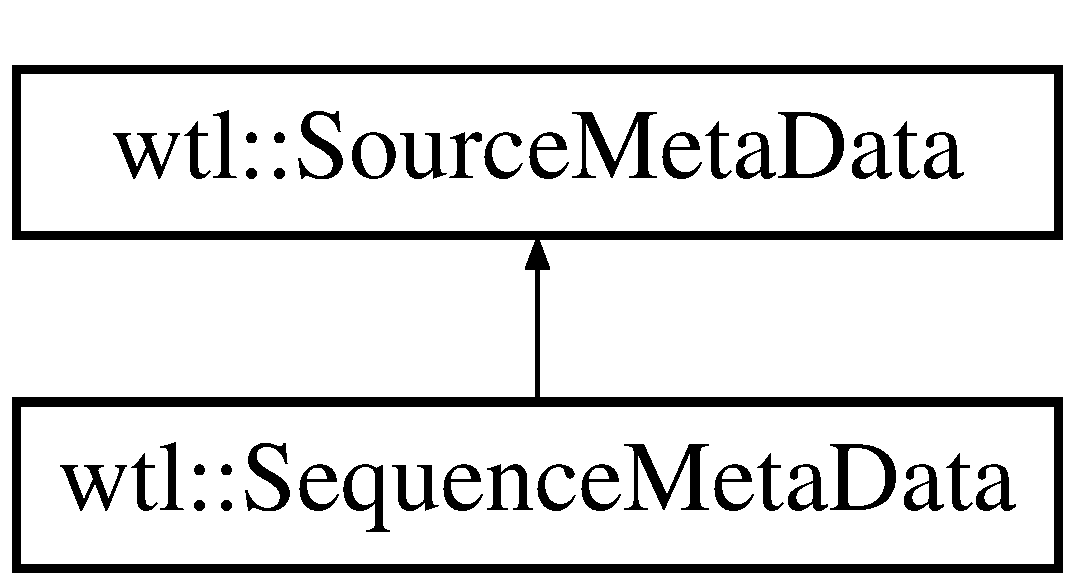
\includegraphics[height=2.000000cm]{classwtl_1_1_sequence_meta_data}
\end{center}
\end{figure}
\subsection*{Public Member Functions}
\begin{DoxyCompactItemize}
\item 
\hyperlink{classwtl_1_1_sequence_meta_data_a309c905124f9595f60aa2aff5ac593c1}{Sequence\+Meta\+Data} ()
\item 
int \hyperlink{classwtl_1_1_sequence_meta_data_aee08a065e63606f91ee12526a4e53b3f}{get\+Frame\+Span} () const
\begin{DoxyCompactList}\small\item\em Sequence frame span. \end{DoxyCompactList}\item 
int \hyperlink{classwtl_1_1_sequence_meta_data_ad9793ec615f6544465c30c150182a4e3}{get\+Frame\+Rate} () const
\begin{DoxyCompactList}\small\item\em Sequence frame rate. \end{DoxyCompactList}\item 
int \hyperlink{classwtl_1_1_sequence_meta_data_ae2883595f742f14a43447a9d2c7fcc8c}{get\+Duration} () const
\begin{DoxyCompactList}\small\item\em Total sequence duration. \end{DoxyCompactList}\item 
int \hyperlink{classwtl_1_1_sequence_meta_data_a95f60019209c2778c8a723d4d5c8fc85}{get\+Frame\+Size} () const
\begin{DoxyCompactList}\small\item\em Sequence Frame Size. \end{DoxyCompactList}\item 
int \hyperlink{classwtl_1_1_sequence_meta_data_a24e3ad706253552c32204774227aefd3}{get\+File\+Size} () const
\begin{DoxyCompactList}\small\item\em Sequence file size. \end{DoxyCompactList}\item 
int \hyperlink{classwtl_1_1_sequence_meta_data_a640215e7856760949b17be5e2131e2f8}{get\+Number\+Of\+Frames} () const
\begin{DoxyCompactList}\small\item\em Number of frames sequence constists of. \end{DoxyCompactList}\end{DoxyCompactItemize}
\subsection*{Friends}
\begin{DoxyCompactItemize}
\item 
class \hyperlink{classwtl_1_1_sequence_meta_data_a89f52b56f7155da8da3c26ad5feb1bcc}{F\+F\+F\+File\+Manager}
\end{DoxyCompactItemize}
\subsection*{Additional Inherited Members}


\subsection{Detailed Description}
Derived class for sequence metadata. 

\subsection{Constructor \& Destructor Documentation}
\mbox{\Hypertarget{classwtl_1_1_sequence_meta_data_a309c905124f9595f60aa2aff5ac593c1}\label{classwtl_1_1_sequence_meta_data_a309c905124f9595f60aa2aff5ac593c1}} 
\index{wtl\+::\+Sequence\+Meta\+Data@{wtl\+::\+Sequence\+Meta\+Data}!Sequence\+Meta\+Data@{Sequence\+Meta\+Data}}
\index{Sequence\+Meta\+Data@{Sequence\+Meta\+Data}!wtl\+::\+Sequence\+Meta\+Data@{wtl\+::\+Sequence\+Meta\+Data}}
\subsubsection{\texorpdfstring{Sequence\+Meta\+Data()}{SequenceMetaData()}}
{\footnotesize\ttfamily wtl\+::\+Sequence\+Meta\+Data\+::\+Sequence\+Meta\+Data (\begin{DoxyParamCaption}{ }\end{DoxyParamCaption})}



\subsection{Member Function Documentation}
\mbox{\Hypertarget{classwtl_1_1_sequence_meta_data_ae2883595f742f14a43447a9d2c7fcc8c}\label{classwtl_1_1_sequence_meta_data_ae2883595f742f14a43447a9d2c7fcc8c}} 
\index{wtl\+::\+Sequence\+Meta\+Data@{wtl\+::\+Sequence\+Meta\+Data}!get\+Duration@{get\+Duration}}
\index{get\+Duration@{get\+Duration}!wtl\+::\+Sequence\+Meta\+Data@{wtl\+::\+Sequence\+Meta\+Data}}
\subsubsection{\texorpdfstring{get\+Duration()}{getDuration()}}
{\footnotesize\ttfamily int wtl\+::\+Sequence\+Meta\+Data\+::get\+Duration (\begin{DoxyParamCaption}{ }\end{DoxyParamCaption}) const}



Total sequence duration. 

\begin{DoxyReturn}{Returns}
Sequence duration in miliseconds. 
\end{DoxyReturn}
\mbox{\Hypertarget{classwtl_1_1_sequence_meta_data_a24e3ad706253552c32204774227aefd3}\label{classwtl_1_1_sequence_meta_data_a24e3ad706253552c32204774227aefd3}} 
\index{wtl\+::\+Sequence\+Meta\+Data@{wtl\+::\+Sequence\+Meta\+Data}!get\+File\+Size@{get\+File\+Size}}
\index{get\+File\+Size@{get\+File\+Size}!wtl\+::\+Sequence\+Meta\+Data@{wtl\+::\+Sequence\+Meta\+Data}}
\subsubsection{\texorpdfstring{get\+File\+Size()}{getFileSize()}}
{\footnotesize\ttfamily int wtl\+::\+Sequence\+Meta\+Data\+::get\+File\+Size (\begin{DoxyParamCaption}{ }\end{DoxyParamCaption}) const}



Sequence file size. 

\begin{DoxyReturn}{Returns}
Size of while file in bytes. 
\end{DoxyReturn}
\mbox{\Hypertarget{classwtl_1_1_sequence_meta_data_ad9793ec615f6544465c30c150182a4e3}\label{classwtl_1_1_sequence_meta_data_ad9793ec615f6544465c30c150182a4e3}} 
\index{wtl\+::\+Sequence\+Meta\+Data@{wtl\+::\+Sequence\+Meta\+Data}!get\+Frame\+Rate@{get\+Frame\+Rate}}
\index{get\+Frame\+Rate@{get\+Frame\+Rate}!wtl\+::\+Sequence\+Meta\+Data@{wtl\+::\+Sequence\+Meta\+Data}}
\subsubsection{\texorpdfstring{get\+Frame\+Rate()}{getFrameRate()}}
{\footnotesize\ttfamily int wtl\+::\+Sequence\+Meta\+Data\+::get\+Frame\+Rate (\begin{DoxyParamCaption}{ }\end{DoxyParamCaption}) const}



Sequence frame rate. 

\begin{DoxyReturn}{Returns}
Number of frames per second. 
\end{DoxyReturn}
\mbox{\Hypertarget{classwtl_1_1_sequence_meta_data_a95f60019209c2778c8a723d4d5c8fc85}\label{classwtl_1_1_sequence_meta_data_a95f60019209c2778c8a723d4d5c8fc85}} 
\index{wtl\+::\+Sequence\+Meta\+Data@{wtl\+::\+Sequence\+Meta\+Data}!get\+Frame\+Size@{get\+Frame\+Size}}
\index{get\+Frame\+Size@{get\+Frame\+Size}!wtl\+::\+Sequence\+Meta\+Data@{wtl\+::\+Sequence\+Meta\+Data}}
\subsubsection{\texorpdfstring{get\+Frame\+Size()}{getFrameSize()}}
{\footnotesize\ttfamily int wtl\+::\+Sequence\+Meta\+Data\+::get\+Frame\+Size (\begin{DoxyParamCaption}{ }\end{DoxyParamCaption}) const}



Sequence Frame Size. 

\begin{DoxyReturn}{Returns}
Size of one frame in bytes. 
\end{DoxyReturn}
\mbox{\Hypertarget{classwtl_1_1_sequence_meta_data_aee08a065e63606f91ee12526a4e53b3f}\label{classwtl_1_1_sequence_meta_data_aee08a065e63606f91ee12526a4e53b3f}} 
\index{wtl\+::\+Sequence\+Meta\+Data@{wtl\+::\+Sequence\+Meta\+Data}!get\+Frame\+Span@{get\+Frame\+Span}}
\index{get\+Frame\+Span@{get\+Frame\+Span}!wtl\+::\+Sequence\+Meta\+Data@{wtl\+::\+Sequence\+Meta\+Data}}
\subsubsection{\texorpdfstring{get\+Frame\+Span()}{getFrameSpan()}}
{\footnotesize\ttfamily int wtl\+::\+Sequence\+Meta\+Data\+::get\+Frame\+Span (\begin{DoxyParamCaption}{ }\end{DoxyParamCaption}) const}



Sequence frame span. 

\begin{DoxyReturn}{Returns}
Duration of one frame of sequence in miliseconds. 
\end{DoxyReturn}
\mbox{\Hypertarget{classwtl_1_1_sequence_meta_data_a640215e7856760949b17be5e2131e2f8}\label{classwtl_1_1_sequence_meta_data_a640215e7856760949b17be5e2131e2f8}} 
\index{wtl\+::\+Sequence\+Meta\+Data@{wtl\+::\+Sequence\+Meta\+Data}!get\+Number\+Of\+Frames@{get\+Number\+Of\+Frames}}
\index{get\+Number\+Of\+Frames@{get\+Number\+Of\+Frames}!wtl\+::\+Sequence\+Meta\+Data@{wtl\+::\+Sequence\+Meta\+Data}}
\subsubsection{\texorpdfstring{get\+Number\+Of\+Frames()}{getNumberOfFrames()}}
{\footnotesize\ttfamily int wtl\+::\+Sequence\+Meta\+Data\+::get\+Number\+Of\+Frames (\begin{DoxyParamCaption}{ }\end{DoxyParamCaption}) const}



Number of frames sequence constists of. 

\begin{DoxyReturn}{Returns}
Number of frames. 
\end{DoxyReturn}


\subsection{Friends And Related Function Documentation}
\mbox{\Hypertarget{classwtl_1_1_sequence_meta_data_a89f52b56f7155da8da3c26ad5feb1bcc}\label{classwtl_1_1_sequence_meta_data_a89f52b56f7155da8da3c26ad5feb1bcc}} 
\index{wtl\+::\+Sequence\+Meta\+Data@{wtl\+::\+Sequence\+Meta\+Data}!F\+F\+F\+File\+Manager@{F\+F\+F\+File\+Manager}}
\index{F\+F\+F\+File\+Manager@{F\+F\+F\+File\+Manager}!wtl\+::\+Sequence\+Meta\+Data@{wtl\+::\+Sequence\+Meta\+Data}}
\subsubsection{\texorpdfstring{F\+F\+F\+File\+Manager}{FFFFileManager}}
{\footnotesize\ttfamily friend class F\+F\+F\+File\+Manager\hspace{0.3cm}{\ttfamily [friend]}}


\hypertarget{classwtl_1_1_sequence_radiometric}{}\section{wtl\+:\+:Sequence\+Radiometric Class Reference}
\label{classwtl_1_1_sequence_radiometric}\index{wtl\+::\+Sequence\+Radiometric@{wtl\+::\+Sequence\+Radiometric}}


Represents a radiometric sequence.  


Inheritance diagram for wtl\+:\+:Sequence\+Radiometric\+:\begin{figure}[H]
\begin{center}
\leavevmode
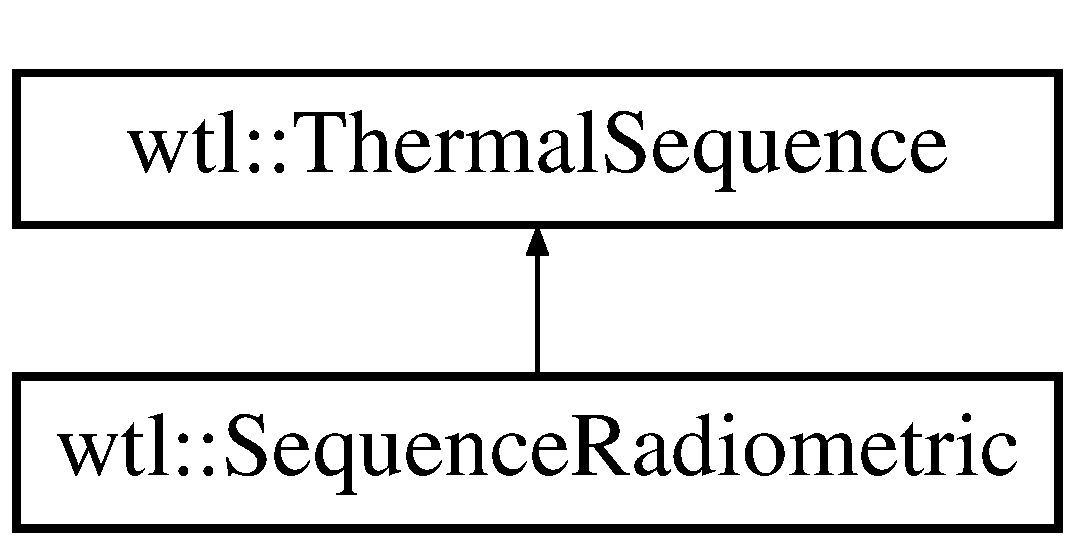
\includegraphics[height=2.000000cm]{classwtl_1_1_sequence_radiometric}
\end{center}
\end{figure}
\subsection*{Public Member Functions}
\begin{DoxyCompactItemize}
\item 
\hyperlink{classwtl_1_1_sequence_radiometric_a2cc32b5a5bad40a78f78aa1388b98fff}{Sequence\+Radiometric} (const \hyperlink{classwtl_1_1_sequence_radiometric}{Sequence\+Radiometric} \&x)=delete
\begin{DoxyCompactList}\small\item\em Copy constructor. \end{DoxyCompactList}\item 
\hyperlink{classwtl_1_1_sequence_radiometric_a0512cf0918f1fcc9ce2d6d23bb3db3ef}{$\sim$\+Sequence\+Radiometric} ()
\begin{DoxyCompactList}\small\item\em Class destructor. \end{DoxyCompactList}\item 
\hyperlink{classwtl_1_1_sequence_radiometric}{Sequence\+Radiometric} \& \hyperlink{classwtl_1_1_sequence_radiometric_ae322c5199985048182697285611c0958}{operator=} (const \hyperlink{classwtl_1_1_sequence_radiometric}{Sequence\+Radiometric} \&x)=delete
\begin{DoxyCompactList}\small\item\em Assignment operator. \end{DoxyCompactList}\item 
std\+::shared\+\_\+ptr$<$ \hyperlink{classwtl_1_1_image_radiometric}{wtl\+::\+Image\+Radiometric} $>$ \hyperlink{classwtl_1_1_sequence_radiometric_a89c1f04092c4b14814693c95b753bbc3}{operator\mbox{[}$\,$\mbox{]}} (size\+\_\+t index)
\begin{DoxyCompactList}\small\item\em Subscription operator. \end{DoxyCompactList}\item 
const std\+::shared\+\_\+ptr$<$ \hyperlink{classwtl_1_1_image_radiometric}{wtl\+::\+Image\+Radiometric} $>$ \hyperlink{classwtl_1_1_sequence_radiometric_afb8a7fd35e6c4b10406953a12c4564fe}{operator\mbox{[}$\,$\mbox{]}} (size\+\_\+t index) const
\begin{DoxyCompactList}\small\item\em Constant Subscription operator. \end{DoxyCompactList}\item 
std\+::shared\+\_\+ptr$<$ \hyperlink{classwtl_1_1_image_radiometric}{wtl\+::\+Image\+Radiometric} $>$ \hyperlink{classwtl_1_1_sequence_radiometric_acff97bda5576bfb082cc5708c9a35200}{at} (int index)
\begin{DoxyCompactList}\small\item\em Returns radiometric image representation of frame at given position.\+Only for sequences with temperature data. \end{DoxyCompactList}\item 
std\+::shared\+\_\+ptr$<$ \hyperlink{classwtl_1_1_thermal_image}{wtl\+::\+Thermal\+Image} $>$ \hyperlink{classwtl_1_1_sequence_radiometric_ae7b8f68b95bdda29cd202570c4fb9fbd}{thermal\+At} (int index) const override
\begin{DoxyCompactList}\small\item\em Returns thermal image representation of frame at given position.\+Only for sequences with temperature data. \end{DoxyCompactList}\item 
std\+::shared\+\_\+ptr$<$ \hyperlink{classwtl_1_1_image_radiometric}{wtl\+::\+Image\+Radiometric} $>$ \hyperlink{classwtl_1_1_sequence_radiometric_a3b465540b5cbc1a7f0dfd1f6d91aa7d1}{radiometric\+At} (int index) const
\begin{DoxyCompactList}\small\item\em Returns thermal image representation of frame at given position.\+Only for sequences with temperature data. \end{DoxyCompactList}\item 
std\+::shared\+\_\+ptr$<$ uint8\+\_\+t $>$ \hyperlink{classwtl_1_1_sequence_radiometric_af0503fb4a89d9a356a4a68bad6da976d}{get\+R\+G\+B\+Frame\+At} (int index)
\begin{DoxyCompactList}\small\item\em Get rgb representation of an frame. \end{DoxyCompactList}\item 
std\+::shared\+\_\+ptr$<$ uint8\+\_\+t $>$ \hyperlink{classwtl_1_1_sequence_radiometric_a04ca24ba12175157835a6f2cb8495971}{get\+R\+G\+B\+Frame\+With\+Overlay\+At} (int index)
\begin{DoxyCompactList}\small\item\em Get rgb representation of an frame \hyperlink{classwtl_1_1_alarms}{Alarms} and measurements overlay is added to the image. \end{DoxyCompactList}\item 
std\+::shared\+\_\+ptr$<$ \hyperlink{classwtl_1_1_measurements}{Measurements} $>$ \hyperlink{classwtl_1_1_sequence_radiometric_a4084caa5e30330375300173b4b0582d0}{get\+Measurements} ()
\begin{DoxyCompactList}\small\item\em Get \hyperlink{classwtl_1_1_measurements}{Measurements}. \end{DoxyCompactList}\item 
std\+::shared\+\_\+ptr$<$ \hyperlink{classwtl_1_1_alarms}{Alarms} $>$ \hyperlink{classwtl_1_1_sequence_radiometric_a11b13d272a8674a3cdccfeb2ed3400fe}{get\+Alarms} ()
\begin{DoxyCompactList}\small\item\em Get \hyperlink{classwtl_1_1_alarms}{Alarms}. \end{DoxyCompactList}\item 
float \hyperlink{classwtl_1_1_sequence_radiometric_a3e944251c9a88be6f5b8cf5f41ffd462}{get\+Palette\+Max\+Temperature} () const
\begin{DoxyCompactList}\small\item\em get\+Palette\+Max\+Temperature \end{DoxyCompactList}\item 
float \hyperlink{classwtl_1_1_sequence_radiometric_a18e8bdc19c4d9e8794653da24db46b70}{get\+Palette\+Min\+Temperature} () const
\begin{DoxyCompactList}\small\item\em get\+Palette\+Min\+Temperature \end{DoxyCompactList}\item 
void \hyperlink{classwtl_1_1_sequence_radiometric_a7d1489f923aeffa694826ea063724251}{set\+Manual\+Max} (float value)
\begin{DoxyCompactList}\small\item\em Set temperature used as maximum for palette. \end{DoxyCompactList}\item 
void \hyperlink{classwtl_1_1_sequence_radiometric_ad5fc50b7c210bc5d2a914ba1c0b47a3c}{set\+Manual\+Min} (float value)
\begin{DoxyCompactList}\small\item\em Set temperature used as minimium for palette. \end{DoxyCompactList}\item 
void \hyperlink{classwtl_1_1_sequence_radiometric_a3faab55fbc056ae2a50f690d78588095}{set\+Emissivity} (double value)
\begin{DoxyCompactList}\small\item\em Set emissivity of objects on an scene. \end{DoxyCompactList}\item 
void \hyperlink{classwtl_1_1_sequence_radiometric_aead15ea790587175b1db26a0859cc51d}{set\+Reflected\+Temp} (double value)
\begin{DoxyCompactList}\small\item\em Set Reflected Temperature of objects on an scene. \end{DoxyCompactList}\item 
void \hyperlink{classwtl_1_1_sequence_radiometric_ac98bfc0193618acc5d62518fb058736b}{set\+Atm\+Temp} (double value)
\begin{DoxyCompactList}\small\item\em Set Atmospheric Temperature. \end{DoxyCompactList}\item 
void \hyperlink{classwtl_1_1_sequence_radiometric_ae34dbec81e6a10de1456e3b4688cfe3c}{set\+Extern\+Optic\+Temp} (double value)
\begin{DoxyCompactList}\small\item\em Set External Optics Temperature. \end{DoxyCompactList}\item 
void \hyperlink{classwtl_1_1_sequence_radiometric_a4b9f85995050a4a683fdd0eed97bbee4}{set\+Object\+Distance} (double value)
\begin{DoxyCompactList}\small\item\em Set distance to objects in scene. \end{DoxyCompactList}\item 
void \hyperlink{classwtl_1_1_sequence_radiometric_a4d8e72885a532ca7f69a08f81f6595cd}{set\+Extern\+Optic\+Trans} (double value)
\begin{DoxyCompactList}\small\item\em Set External Optics Transition. \end{DoxyCompactList}\item 
void \hyperlink{classwtl_1_1_sequence_radiometric_a87da464d019d313a67609a7c99ea8e4e}{set\+Humidity} (double value)
\begin{DoxyCompactList}\small\item\em Set humidity. \end{DoxyCompactList}\item 
double \hyperlink{classwtl_1_1_sequence_radiometric_ad063c67b479c8fb33a77205ecfbd48d7}{get\+Emissivity} ()
\begin{DoxyCompactList}\small\item\em get\+Emissivity \end{DoxyCompactList}\item 
double \hyperlink{classwtl_1_1_sequence_radiometric_a1ea0a824608afd40f7dfda8c8539a269}{get\+Reflected\+Temp} ()
\begin{DoxyCompactList}\small\item\em get\+Reflected\+Temp \end{DoxyCompactList}\item 
double \hyperlink{classwtl_1_1_sequence_radiometric_adb55fc5e945d0a7972b0b2ffda3e8c36}{get\+Atm\+Temp} ()
\begin{DoxyCompactList}\small\item\em get\+Atm\+Temp \end{DoxyCompactList}\item 
double \hyperlink{classwtl_1_1_sequence_radiometric_a98d3f1c3318a7e5ffb9812b693bb49d0}{get\+Extern\+Optic\+Temp} ()
\begin{DoxyCompactList}\small\item\em get\+Extern\+Optic\+Temp \end{DoxyCompactList}\item 
double \hyperlink{classwtl_1_1_sequence_radiometric_a65570c0765b96e161b260d1582379e0a}{get\+Object\+Distance} ()
\begin{DoxyCompactList}\small\item\em get\+Object\+Distance \end{DoxyCompactList}\item 
double \hyperlink{classwtl_1_1_sequence_radiometric_ad07e40b2ad7f0dcb1b0db5de47bfebb0}{get\+Extern\+Optic\+Trans} ()
\begin{DoxyCompactList}\small\item\em get\+Extern\+Optic\+Trans \end{DoxyCompactList}\item 
double \hyperlink{classwtl_1_1_sequence_radiometric_a5c45c9e5200e04e67fa65cb56f1f17dc}{get\+Humidity} ()
\begin{DoxyCompactList}\small\item\em get\+Humidity \end{DoxyCompactList}\item 
bool \hyperlink{classwtl_1_1_sequence_radiometric_aa0b063cfe218f95cd57412344d4f9a04}{is\+Radiometric\+Sequence} () const
\begin{DoxyCompactList}\small\item\em Decide whether thermal sequence instance contains radiometric temperature data. \end{DoxyCompactList}\item 
void \hyperlink{classwtl_1_1_sequence_radiometric_a3cca0f0bbabe787926910bcedd9307ea}{add\+Roi\+To\+Sequence} (std\+::shared\+\_\+ptr$<$ \hyperlink{structwtl_1_1_roi_struct}{Roi\+Struct} $>$ roi)
\begin{DoxyCompactList}\small\item\em Add R\+OI item to sequence. \end{DoxyCompactList}\item 
void \hyperlink{classwtl_1_1_sequence_radiometric_ab42fcdd2531eb26af5f4801e1c8f171b}{update\+Custom\+Params\+Roi} (\hyperlink{structwtl_1_1_roi_struct}{Roi\+Struct} \&roi, bool custom\+Params, float emissivity, float refl\+Temp, float distance)
\begin{DoxyCompactList}\small\item\em update\+Custom\+Params\+Roi \end{DoxyCompactList}\item 
void \hyperlink{classwtl_1_1_sequence_radiometric_a3117b737de49b7f1b0963a233fc6e463}{add\+Alarm\+To\+Sequence} (std\+::shared\+\_\+ptr$<$ \hyperlink{structwtl_1_1_alarm_struct}{Alarm\+Struct} $>$ alarm)
\begin{DoxyCompactList}\small\item\em Add Alarm item to sequence. \end{DoxyCompactList}\end{DoxyCompactItemize}
\subsection*{Friends}
\begin{DoxyCompactItemize}
\item 
class \hyperlink{classwtl_1_1_sequence_radiometric_a5baf0a1f190dbaabf7033b4ba92f4c81}{Center}
\item 
class \hyperlink{classwtl_1_1_sequence_radiometric_a89f52b56f7155da8da3c26ad5feb1bcc}{F\+F\+F\+File\+Manager}
\end{DoxyCompactItemize}
\subsection*{Additional Inherited Members}


\subsection{Detailed Description}
Represents a radiometric sequence. 

Provides interface for extracting and saving data to sequences of thermal images. Sequence is processed as a stream of thermal images. 

\subsection{Constructor \& Destructor Documentation}
\mbox{\Hypertarget{classwtl_1_1_sequence_radiometric_a2cc32b5a5bad40a78f78aa1388b98fff}\label{classwtl_1_1_sequence_radiometric_a2cc32b5a5bad40a78f78aa1388b98fff}} 
\index{wtl\+::\+Sequence\+Radiometric@{wtl\+::\+Sequence\+Radiometric}!Sequence\+Radiometric@{Sequence\+Radiometric}}
\index{Sequence\+Radiometric@{Sequence\+Radiometric}!wtl\+::\+Sequence\+Radiometric@{wtl\+::\+Sequence\+Radiometric}}
\subsubsection{\texorpdfstring{Sequence\+Radiometric()}{SequenceRadiometric()}}
{\footnotesize\ttfamily wtl\+::\+Sequence\+Radiometric\+::\+Sequence\+Radiometric (\begin{DoxyParamCaption}\item[{const \hyperlink{classwtl_1_1_sequence_radiometric}{Sequence\+Radiometric} \&}]{x }\end{DoxyParamCaption})\hspace{0.3cm}{\ttfamily [delete]}}



Copy constructor. 


\begin{DoxyParams}{Parameters}
{\em x} & Source thermal sequence. \\
\hline
\end{DoxyParams}
\mbox{\Hypertarget{classwtl_1_1_sequence_radiometric_a0512cf0918f1fcc9ce2d6d23bb3db3ef}\label{classwtl_1_1_sequence_radiometric_a0512cf0918f1fcc9ce2d6d23bb3db3ef}} 
\index{wtl\+::\+Sequence\+Radiometric@{wtl\+::\+Sequence\+Radiometric}!````~Sequence\+Radiometric@{$\sim$\+Sequence\+Radiometric}}
\index{````~Sequence\+Radiometric@{$\sim$\+Sequence\+Radiometric}!wtl\+::\+Sequence\+Radiometric@{wtl\+::\+Sequence\+Radiometric}}
\subsubsection{\texorpdfstring{$\sim$\+Sequence\+Radiometric()}{~SequenceRadiometric()}}
{\footnotesize\ttfamily wtl\+::\+Sequence\+Radiometric\+::$\sim$\+Sequence\+Radiometric (\begin{DoxyParamCaption}{ }\end{DoxyParamCaption})}



Class destructor. 



\subsection{Member Function Documentation}
\mbox{\Hypertarget{classwtl_1_1_sequence_radiometric_a3117b737de49b7f1b0963a233fc6e463}\label{classwtl_1_1_sequence_radiometric_a3117b737de49b7f1b0963a233fc6e463}} 
\index{wtl\+::\+Sequence\+Radiometric@{wtl\+::\+Sequence\+Radiometric}!add\+Alarm\+To\+Sequence@{add\+Alarm\+To\+Sequence}}
\index{add\+Alarm\+To\+Sequence@{add\+Alarm\+To\+Sequence}!wtl\+::\+Sequence\+Radiometric@{wtl\+::\+Sequence\+Radiometric}}
\subsubsection{\texorpdfstring{add\+Alarm\+To\+Sequence()}{addAlarmToSequence()}}
{\footnotesize\ttfamily void wtl\+::\+Sequence\+Radiometric\+::add\+Alarm\+To\+Sequence (\begin{DoxyParamCaption}\item[{std\+::shared\+\_\+ptr$<$ \hyperlink{structwtl_1_1_alarm_struct}{Alarm\+Struct} $>$}]{alarm }\end{DoxyParamCaption})}



Add Alarm item to sequence. 


\begin{DoxyParams}{Parameters}
{\em alarm} & Alarm item. \\
\hline
\end{DoxyParams}
\mbox{\Hypertarget{classwtl_1_1_sequence_radiometric_a3cca0f0bbabe787926910bcedd9307ea}\label{classwtl_1_1_sequence_radiometric_a3cca0f0bbabe787926910bcedd9307ea}} 
\index{wtl\+::\+Sequence\+Radiometric@{wtl\+::\+Sequence\+Radiometric}!add\+Roi\+To\+Sequence@{add\+Roi\+To\+Sequence}}
\index{add\+Roi\+To\+Sequence@{add\+Roi\+To\+Sequence}!wtl\+::\+Sequence\+Radiometric@{wtl\+::\+Sequence\+Radiometric}}
\subsubsection{\texorpdfstring{add\+Roi\+To\+Sequence()}{addRoiToSequence()}}
{\footnotesize\ttfamily void wtl\+::\+Sequence\+Radiometric\+::add\+Roi\+To\+Sequence (\begin{DoxyParamCaption}\item[{std\+::shared\+\_\+ptr$<$ \hyperlink{structwtl_1_1_roi_struct}{Roi\+Struct} $>$}]{roi }\end{DoxyParamCaption})}



Add R\+OI item to sequence. 


\begin{DoxyParams}{Parameters}
{\em roi} & R\+OI item. \\
\hline
\end{DoxyParams}
\mbox{\Hypertarget{classwtl_1_1_sequence_radiometric_acff97bda5576bfb082cc5708c9a35200}\label{classwtl_1_1_sequence_radiometric_acff97bda5576bfb082cc5708c9a35200}} 
\index{wtl\+::\+Sequence\+Radiometric@{wtl\+::\+Sequence\+Radiometric}!at@{at}}
\index{at@{at}!wtl\+::\+Sequence\+Radiometric@{wtl\+::\+Sequence\+Radiometric}}
\subsubsection{\texorpdfstring{at()}{at()}}
{\footnotesize\ttfamily std\+::shared\+\_\+ptr$<$ \hyperlink{classwtl_1_1_image_radiometric}{wtl\+::\+Image\+Radiometric} $>$ wtl\+::\+Sequence\+Radiometric\+::at (\begin{DoxyParamCaption}\item[{int}]{index }\end{DoxyParamCaption})}



Returns radiometric image representation of frame at given position.\+Only for sequences with temperature data. 

\mbox{\Hypertarget{classwtl_1_1_sequence_radiometric_a11b13d272a8674a3cdccfeb2ed3400fe}\label{classwtl_1_1_sequence_radiometric_a11b13d272a8674a3cdccfeb2ed3400fe}} 
\index{wtl\+::\+Sequence\+Radiometric@{wtl\+::\+Sequence\+Radiometric}!get\+Alarms@{get\+Alarms}}
\index{get\+Alarms@{get\+Alarms}!wtl\+::\+Sequence\+Radiometric@{wtl\+::\+Sequence\+Radiometric}}
\subsubsection{\texorpdfstring{get\+Alarms()}{getAlarms()}}
{\footnotesize\ttfamily std\+::shared\+\_\+ptr$<$ \hyperlink{classwtl_1_1_alarms}{wtl\+::\+Alarms} $>$ wtl\+::\+Sequence\+Radiometric\+::get\+Alarms (\begin{DoxyParamCaption}{ }\end{DoxyParamCaption})}



Get \hyperlink{classwtl_1_1_alarms}{Alarms}. 

\begin{DoxyReturn}{Returns}
Shared pointer to all the alarms present in a source 
\end{DoxyReturn}
\mbox{\Hypertarget{classwtl_1_1_sequence_radiometric_adb55fc5e945d0a7972b0b2ffda3e8c36}\label{classwtl_1_1_sequence_radiometric_adb55fc5e945d0a7972b0b2ffda3e8c36}} 
\index{wtl\+::\+Sequence\+Radiometric@{wtl\+::\+Sequence\+Radiometric}!get\+Atm\+Temp@{get\+Atm\+Temp}}
\index{get\+Atm\+Temp@{get\+Atm\+Temp}!wtl\+::\+Sequence\+Radiometric@{wtl\+::\+Sequence\+Radiometric}}
\subsubsection{\texorpdfstring{get\+Atm\+Temp()}{getAtmTemp()}}
{\footnotesize\ttfamily double wtl\+::\+Sequence\+Radiometric\+::get\+Atm\+Temp (\begin{DoxyParamCaption}{ }\end{DoxyParamCaption})}



get\+Atm\+Temp 

\begin{DoxyReturn}{Returns}
Atmospheric temperature 
\end{DoxyReturn}
\mbox{\Hypertarget{classwtl_1_1_sequence_radiometric_ad063c67b479c8fb33a77205ecfbd48d7}\label{classwtl_1_1_sequence_radiometric_ad063c67b479c8fb33a77205ecfbd48d7}} 
\index{wtl\+::\+Sequence\+Radiometric@{wtl\+::\+Sequence\+Radiometric}!get\+Emissivity@{get\+Emissivity}}
\index{get\+Emissivity@{get\+Emissivity}!wtl\+::\+Sequence\+Radiometric@{wtl\+::\+Sequence\+Radiometric}}
\subsubsection{\texorpdfstring{get\+Emissivity()}{getEmissivity()}}
{\footnotesize\ttfamily double wtl\+::\+Sequence\+Radiometric\+::get\+Emissivity (\begin{DoxyParamCaption}{ }\end{DoxyParamCaption})}



get\+Emissivity 

\begin{DoxyReturn}{Returns}
Sequence emissivity 
\end{DoxyReturn}
\mbox{\Hypertarget{classwtl_1_1_sequence_radiometric_a98d3f1c3318a7e5ffb9812b693bb49d0}\label{classwtl_1_1_sequence_radiometric_a98d3f1c3318a7e5ffb9812b693bb49d0}} 
\index{wtl\+::\+Sequence\+Radiometric@{wtl\+::\+Sequence\+Radiometric}!get\+Extern\+Optic\+Temp@{get\+Extern\+Optic\+Temp}}
\index{get\+Extern\+Optic\+Temp@{get\+Extern\+Optic\+Temp}!wtl\+::\+Sequence\+Radiometric@{wtl\+::\+Sequence\+Radiometric}}
\subsubsection{\texorpdfstring{get\+Extern\+Optic\+Temp()}{getExternOpticTemp()}}
{\footnotesize\ttfamily double wtl\+::\+Sequence\+Radiometric\+::get\+Extern\+Optic\+Temp (\begin{DoxyParamCaption}{ }\end{DoxyParamCaption})}



get\+Extern\+Optic\+Temp 

\begin{DoxyReturn}{Returns}
External Optics Temperature 
\end{DoxyReturn}
\mbox{\Hypertarget{classwtl_1_1_sequence_radiometric_ad07e40b2ad7f0dcb1b0db5de47bfebb0}\label{classwtl_1_1_sequence_radiometric_ad07e40b2ad7f0dcb1b0db5de47bfebb0}} 
\index{wtl\+::\+Sequence\+Radiometric@{wtl\+::\+Sequence\+Radiometric}!get\+Extern\+Optic\+Trans@{get\+Extern\+Optic\+Trans}}
\index{get\+Extern\+Optic\+Trans@{get\+Extern\+Optic\+Trans}!wtl\+::\+Sequence\+Radiometric@{wtl\+::\+Sequence\+Radiometric}}
\subsubsection{\texorpdfstring{get\+Extern\+Optic\+Trans()}{getExternOpticTrans()}}
{\footnotesize\ttfamily double wtl\+::\+Sequence\+Radiometric\+::get\+Extern\+Optic\+Trans (\begin{DoxyParamCaption}{ }\end{DoxyParamCaption})}



get\+Extern\+Optic\+Trans 

\begin{DoxyReturn}{Returns}
External optics transmission 
\end{DoxyReturn}
\mbox{\Hypertarget{classwtl_1_1_sequence_radiometric_a5c45c9e5200e04e67fa65cb56f1f17dc}\label{classwtl_1_1_sequence_radiometric_a5c45c9e5200e04e67fa65cb56f1f17dc}} 
\index{wtl\+::\+Sequence\+Radiometric@{wtl\+::\+Sequence\+Radiometric}!get\+Humidity@{get\+Humidity}}
\index{get\+Humidity@{get\+Humidity}!wtl\+::\+Sequence\+Radiometric@{wtl\+::\+Sequence\+Radiometric}}
\subsubsection{\texorpdfstring{get\+Humidity()}{getHumidity()}}
{\footnotesize\ttfamily double wtl\+::\+Sequence\+Radiometric\+::get\+Humidity (\begin{DoxyParamCaption}{ }\end{DoxyParamCaption})}



get\+Humidity 

\begin{DoxyReturn}{Returns}
Relative humidity 
\end{DoxyReturn}
\mbox{\Hypertarget{classwtl_1_1_sequence_radiometric_a4084caa5e30330375300173b4b0582d0}\label{classwtl_1_1_sequence_radiometric_a4084caa5e30330375300173b4b0582d0}} 
\index{wtl\+::\+Sequence\+Radiometric@{wtl\+::\+Sequence\+Radiometric}!get\+Measurements@{get\+Measurements}}
\index{get\+Measurements@{get\+Measurements}!wtl\+::\+Sequence\+Radiometric@{wtl\+::\+Sequence\+Radiometric}}
\subsubsection{\texorpdfstring{get\+Measurements()}{getMeasurements()}}
{\footnotesize\ttfamily std\+::shared\+\_\+ptr$<$ \hyperlink{classwtl_1_1_measurements}{wtl\+::\+Measurements} $>$ wtl\+::\+Sequence\+Radiometric\+::get\+Measurements (\begin{DoxyParamCaption}{ }\end{DoxyParamCaption})}



Get \hyperlink{classwtl_1_1_measurements}{Measurements}. 

\begin{DoxyReturn}{Returns}
Shared pointer to all the measurements present in a source 
\end{DoxyReturn}
\mbox{\Hypertarget{classwtl_1_1_sequence_radiometric_a65570c0765b96e161b260d1582379e0a}\label{classwtl_1_1_sequence_radiometric_a65570c0765b96e161b260d1582379e0a}} 
\index{wtl\+::\+Sequence\+Radiometric@{wtl\+::\+Sequence\+Radiometric}!get\+Object\+Distance@{get\+Object\+Distance}}
\index{get\+Object\+Distance@{get\+Object\+Distance}!wtl\+::\+Sequence\+Radiometric@{wtl\+::\+Sequence\+Radiometric}}
\subsubsection{\texorpdfstring{get\+Object\+Distance()}{getObjectDistance()}}
{\footnotesize\ttfamily double wtl\+::\+Sequence\+Radiometric\+::get\+Object\+Distance (\begin{DoxyParamCaption}{ }\end{DoxyParamCaption})}



get\+Object\+Distance 

\begin{DoxyReturn}{Returns}
Distance of an captured object 
\end{DoxyReturn}
\mbox{\Hypertarget{classwtl_1_1_sequence_radiometric_a3e944251c9a88be6f5b8cf5f41ffd462}\label{classwtl_1_1_sequence_radiometric_a3e944251c9a88be6f5b8cf5f41ffd462}} 
\index{wtl\+::\+Sequence\+Radiometric@{wtl\+::\+Sequence\+Radiometric}!get\+Palette\+Max\+Temperature@{get\+Palette\+Max\+Temperature}}
\index{get\+Palette\+Max\+Temperature@{get\+Palette\+Max\+Temperature}!wtl\+::\+Sequence\+Radiometric@{wtl\+::\+Sequence\+Radiometric}}
\subsubsection{\texorpdfstring{get\+Palette\+Max\+Temperature()}{getPaletteMaxTemperature()}}
{\footnotesize\ttfamily float wtl\+::\+Sequence\+Radiometric\+::get\+Palette\+Max\+Temperature (\begin{DoxyParamCaption}{ }\end{DoxyParamCaption}) const}



get\+Palette\+Max\+Temperature 

\begin{DoxyReturn}{Returns}

\end{DoxyReturn}
\mbox{\Hypertarget{classwtl_1_1_sequence_radiometric_a18e8bdc19c4d9e8794653da24db46b70}\label{classwtl_1_1_sequence_radiometric_a18e8bdc19c4d9e8794653da24db46b70}} 
\index{wtl\+::\+Sequence\+Radiometric@{wtl\+::\+Sequence\+Radiometric}!get\+Palette\+Min\+Temperature@{get\+Palette\+Min\+Temperature}}
\index{get\+Palette\+Min\+Temperature@{get\+Palette\+Min\+Temperature}!wtl\+::\+Sequence\+Radiometric@{wtl\+::\+Sequence\+Radiometric}}
\subsubsection{\texorpdfstring{get\+Palette\+Min\+Temperature()}{getPaletteMinTemperature()}}
{\footnotesize\ttfamily float wtl\+::\+Sequence\+Radiometric\+::get\+Palette\+Min\+Temperature (\begin{DoxyParamCaption}{ }\end{DoxyParamCaption}) const}



get\+Palette\+Min\+Temperature 

\begin{DoxyReturn}{Returns}

\end{DoxyReturn}
\mbox{\Hypertarget{classwtl_1_1_sequence_radiometric_a1ea0a824608afd40f7dfda8c8539a269}\label{classwtl_1_1_sequence_radiometric_a1ea0a824608afd40f7dfda8c8539a269}} 
\index{wtl\+::\+Sequence\+Radiometric@{wtl\+::\+Sequence\+Radiometric}!get\+Reflected\+Temp@{get\+Reflected\+Temp}}
\index{get\+Reflected\+Temp@{get\+Reflected\+Temp}!wtl\+::\+Sequence\+Radiometric@{wtl\+::\+Sequence\+Radiometric}}
\subsubsection{\texorpdfstring{get\+Reflected\+Temp()}{getReflectedTemp()}}
{\footnotesize\ttfamily double wtl\+::\+Sequence\+Radiometric\+::get\+Reflected\+Temp (\begin{DoxyParamCaption}{ }\end{DoxyParamCaption})}



get\+Reflected\+Temp 

\begin{DoxyReturn}{Returns}
Reflected Temperature 
\end{DoxyReturn}
\mbox{\Hypertarget{classwtl_1_1_sequence_radiometric_af0503fb4a89d9a356a4a68bad6da976d}\label{classwtl_1_1_sequence_radiometric_af0503fb4a89d9a356a4a68bad6da976d}} 
\index{wtl\+::\+Sequence\+Radiometric@{wtl\+::\+Sequence\+Radiometric}!get\+R\+G\+B\+Frame\+At@{get\+R\+G\+B\+Frame\+At}}
\index{get\+R\+G\+B\+Frame\+At@{get\+R\+G\+B\+Frame\+At}!wtl\+::\+Sequence\+Radiometric@{wtl\+::\+Sequence\+Radiometric}}
\subsubsection{\texorpdfstring{get\+R\+G\+B\+Frame\+At()}{getRGBFrameAt()}}
{\footnotesize\ttfamily std\+::shared\+\_\+ptr$<$ uint8\+\_\+t $>$ wtl\+::\+Sequence\+Radiometric\+::get\+R\+G\+B\+Frame\+At (\begin{DoxyParamCaption}\item[{int}]{index }\end{DoxyParamCaption})\hspace{0.3cm}{\ttfamily [virtual]}}



Get rgb representation of an frame. 


\begin{DoxyParams}{Parameters}
{\em index} & Frame number \\
\hline
\end{DoxyParams}
\begin{DoxyReturn}{Returns}
1D array of rgb image data, 8 bits per chanel 
\end{DoxyReturn}


Implements \hyperlink{classwtl_1_1_thermal_sequence_a0d13f29f0f89343516031c5146b62792}{wtl\+::\+Thermal\+Sequence}.

\mbox{\Hypertarget{classwtl_1_1_sequence_radiometric_a04ca24ba12175157835a6f2cb8495971}\label{classwtl_1_1_sequence_radiometric_a04ca24ba12175157835a6f2cb8495971}} 
\index{wtl\+::\+Sequence\+Radiometric@{wtl\+::\+Sequence\+Radiometric}!get\+R\+G\+B\+Frame\+With\+Overlay\+At@{get\+R\+G\+B\+Frame\+With\+Overlay\+At}}
\index{get\+R\+G\+B\+Frame\+With\+Overlay\+At@{get\+R\+G\+B\+Frame\+With\+Overlay\+At}!wtl\+::\+Sequence\+Radiometric@{wtl\+::\+Sequence\+Radiometric}}
\subsubsection{\texorpdfstring{get\+R\+G\+B\+Frame\+With\+Overlay\+At()}{getRGBFrameWithOverlayAt()}}
{\footnotesize\ttfamily std\+::shared\+\_\+ptr$<$ uint8\+\_\+t $>$ wtl\+::\+Sequence\+Radiometric\+::get\+R\+G\+B\+Frame\+With\+Overlay\+At (\begin{DoxyParamCaption}\item[{int}]{index }\end{DoxyParamCaption})}



Get rgb representation of an frame \hyperlink{classwtl_1_1_alarms}{Alarms} and measurements overlay is added to the image. 


\begin{DoxyParams}{Parameters}
{\em index} & Frame number \\
\hline
\end{DoxyParams}
\begin{DoxyReturn}{Returns}
1D array of rgb image data, 8 bits per chanel 
\end{DoxyReturn}
\mbox{\Hypertarget{classwtl_1_1_sequence_radiometric_aa0b063cfe218f95cd57412344d4f9a04}\label{classwtl_1_1_sequence_radiometric_aa0b063cfe218f95cd57412344d4f9a04}} 
\index{wtl\+::\+Sequence\+Radiometric@{wtl\+::\+Sequence\+Radiometric}!is\+Radiometric\+Sequence@{is\+Radiometric\+Sequence}}
\index{is\+Radiometric\+Sequence@{is\+Radiometric\+Sequence}!wtl\+::\+Sequence\+Radiometric@{wtl\+::\+Sequence\+Radiometric}}
\subsubsection{\texorpdfstring{is\+Radiometric\+Sequence()}{isRadiometricSequence()}}
{\footnotesize\ttfamily bool wtl\+::\+Sequence\+Radiometric\+::is\+Radiometric\+Sequence (\begin{DoxyParamCaption}{ }\end{DoxyParamCaption}) const\hspace{0.3cm}{\ttfamily [virtual]}}



Decide whether thermal sequence instance contains radiometric temperature data. 

\begin{DoxyReturn}{Returns}
True if image contains temperature for every pixel 
\end{DoxyReturn}


Implements \hyperlink{classwtl_1_1_thermal_sequence_a572ec84280f0edc98c5ad0c0a0593335}{wtl\+::\+Thermal\+Sequence}.

\mbox{\Hypertarget{classwtl_1_1_sequence_radiometric_ae322c5199985048182697285611c0958}\label{classwtl_1_1_sequence_radiometric_ae322c5199985048182697285611c0958}} 
\index{wtl\+::\+Sequence\+Radiometric@{wtl\+::\+Sequence\+Radiometric}!operator=@{operator=}}
\index{operator=@{operator=}!wtl\+::\+Sequence\+Radiometric@{wtl\+::\+Sequence\+Radiometric}}
\subsubsection{\texorpdfstring{operator=()}{operator=()}}
{\footnotesize\ttfamily \hyperlink{classwtl_1_1_sequence_radiometric}{Sequence\+Radiometric}\& wtl\+::\+Sequence\+Radiometric\+::operator= (\begin{DoxyParamCaption}\item[{const \hyperlink{classwtl_1_1_sequence_radiometric}{Sequence\+Radiometric} \&}]{x }\end{DoxyParamCaption})\hspace{0.3cm}{\ttfamily [delete]}}



Assignment operator. 


\begin{DoxyParams}{Parameters}
{\em x} & Source thermal sequence. \\
\hline
\end{DoxyParams}
\mbox{\Hypertarget{classwtl_1_1_sequence_radiometric_a89c1f04092c4b14814693c95b753bbc3}\label{classwtl_1_1_sequence_radiometric_a89c1f04092c4b14814693c95b753bbc3}} 
\index{wtl\+::\+Sequence\+Radiometric@{wtl\+::\+Sequence\+Radiometric}!operator\mbox{[}\mbox{]}@{operator[]}}
\index{operator\mbox{[}\mbox{]}@{operator[]}!wtl\+::\+Sequence\+Radiometric@{wtl\+::\+Sequence\+Radiometric}}
\subsubsection{\texorpdfstring{operator[]()}{operator[]()}\hspace{0.1cm}{\footnotesize\ttfamily [1/2]}}
{\footnotesize\ttfamily std\+::shared\+\_\+ptr$<$ \hyperlink{classwtl_1_1_image_radiometric}{wtl\+::\+Image\+Radiometric} $>$ wtl\+::\+Sequence\+Radiometric\+::operator\mbox{[}$\,$\mbox{]} (\begin{DoxyParamCaption}\item[{size\+\_\+t}]{index }\end{DoxyParamCaption})}



Subscription operator. 

Enables random access to sequence frames as radiometric images.\+Only for sequences with temperature data. \mbox{\Hypertarget{classwtl_1_1_sequence_radiometric_afb8a7fd35e6c4b10406953a12c4564fe}\label{classwtl_1_1_sequence_radiometric_afb8a7fd35e6c4b10406953a12c4564fe}} 
\index{wtl\+::\+Sequence\+Radiometric@{wtl\+::\+Sequence\+Radiometric}!operator\mbox{[}\mbox{]}@{operator[]}}
\index{operator\mbox{[}\mbox{]}@{operator[]}!wtl\+::\+Sequence\+Radiometric@{wtl\+::\+Sequence\+Radiometric}}
\subsubsection{\texorpdfstring{operator[]()}{operator[]()}\hspace{0.1cm}{\footnotesize\ttfamily [2/2]}}
{\footnotesize\ttfamily const std\+::shared\+\_\+ptr$<$ \hyperlink{classwtl_1_1_image_radiometric}{wtl\+::\+Image\+Radiometric} $>$ wtl\+::\+Sequence\+Radiometric\+::operator\mbox{[}$\,$\mbox{]} (\begin{DoxyParamCaption}\item[{size\+\_\+t}]{index }\end{DoxyParamCaption}) const}



Constant Subscription operator. 

Enables random access to sequence frames as radiometric images. Only for sequences with temperature data. \mbox{\Hypertarget{classwtl_1_1_sequence_radiometric_a3b465540b5cbc1a7f0dfd1f6d91aa7d1}\label{classwtl_1_1_sequence_radiometric_a3b465540b5cbc1a7f0dfd1f6d91aa7d1}} 
\index{wtl\+::\+Sequence\+Radiometric@{wtl\+::\+Sequence\+Radiometric}!radiometric\+At@{radiometric\+At}}
\index{radiometric\+At@{radiometric\+At}!wtl\+::\+Sequence\+Radiometric@{wtl\+::\+Sequence\+Radiometric}}
\subsubsection{\texorpdfstring{radiometric\+At()}{radiometricAt()}}
{\footnotesize\ttfamily std\+::shared\+\_\+ptr$<$ \hyperlink{classwtl_1_1_image_radiometric}{wtl\+::\+Image\+Radiometric} $>$ wtl\+::\+Sequence\+Radiometric\+::radiometric\+At (\begin{DoxyParamCaption}\item[{int}]{index }\end{DoxyParamCaption}) const}



Returns thermal image representation of frame at given position.\+Only for sequences with temperature data. 

Copies thermal data from sequence to this frame which includes recalculation \mbox{\Hypertarget{classwtl_1_1_sequence_radiometric_ac98bfc0193618acc5d62518fb058736b}\label{classwtl_1_1_sequence_radiometric_ac98bfc0193618acc5d62518fb058736b}} 
\index{wtl\+::\+Sequence\+Radiometric@{wtl\+::\+Sequence\+Radiometric}!set\+Atm\+Temp@{set\+Atm\+Temp}}
\index{set\+Atm\+Temp@{set\+Atm\+Temp}!wtl\+::\+Sequence\+Radiometric@{wtl\+::\+Sequence\+Radiometric}}
\subsubsection{\texorpdfstring{set\+Atm\+Temp()}{setAtmTemp()}}
{\footnotesize\ttfamily void wtl\+::\+Sequence\+Radiometric\+::set\+Atm\+Temp (\begin{DoxyParamCaption}\item[{double}]{value }\end{DoxyParamCaption})}



Set Atmospheric Temperature. 


\begin{DoxyParams}{Parameters}
{\em value} & New Atmospheric temperature value. \\
\hline
\end{DoxyParams}
\mbox{\Hypertarget{classwtl_1_1_sequence_radiometric_a3faab55fbc056ae2a50f690d78588095}\label{classwtl_1_1_sequence_radiometric_a3faab55fbc056ae2a50f690d78588095}} 
\index{wtl\+::\+Sequence\+Radiometric@{wtl\+::\+Sequence\+Radiometric}!set\+Emissivity@{set\+Emissivity}}
\index{set\+Emissivity@{set\+Emissivity}!wtl\+::\+Sequence\+Radiometric@{wtl\+::\+Sequence\+Radiometric}}
\subsubsection{\texorpdfstring{set\+Emissivity()}{setEmissivity()}}
{\footnotesize\ttfamily void wtl\+::\+Sequence\+Radiometric\+::set\+Emissivity (\begin{DoxyParamCaption}\item[{double}]{value }\end{DoxyParamCaption})}



Set emissivity of objects on an scene. 


\begin{DoxyParams}{Parameters}
{\em value} & New emissivity value \\
\hline
\end{DoxyParams}
\mbox{\Hypertarget{classwtl_1_1_sequence_radiometric_ae34dbec81e6a10de1456e3b4688cfe3c}\label{classwtl_1_1_sequence_radiometric_ae34dbec81e6a10de1456e3b4688cfe3c}} 
\index{wtl\+::\+Sequence\+Radiometric@{wtl\+::\+Sequence\+Radiometric}!set\+Extern\+Optic\+Temp@{set\+Extern\+Optic\+Temp}}
\index{set\+Extern\+Optic\+Temp@{set\+Extern\+Optic\+Temp}!wtl\+::\+Sequence\+Radiometric@{wtl\+::\+Sequence\+Radiometric}}
\subsubsection{\texorpdfstring{set\+Extern\+Optic\+Temp()}{setExternOpticTemp()}}
{\footnotesize\ttfamily void wtl\+::\+Sequence\+Radiometric\+::set\+Extern\+Optic\+Temp (\begin{DoxyParamCaption}\item[{double}]{value }\end{DoxyParamCaption})}



Set External Optics Temperature. 


\begin{DoxyParams}{Parameters}
{\em value} & New value. \\
\hline
\end{DoxyParams}
\mbox{\Hypertarget{classwtl_1_1_sequence_radiometric_a4d8e72885a532ca7f69a08f81f6595cd}\label{classwtl_1_1_sequence_radiometric_a4d8e72885a532ca7f69a08f81f6595cd}} 
\index{wtl\+::\+Sequence\+Radiometric@{wtl\+::\+Sequence\+Radiometric}!set\+Extern\+Optic\+Trans@{set\+Extern\+Optic\+Trans}}
\index{set\+Extern\+Optic\+Trans@{set\+Extern\+Optic\+Trans}!wtl\+::\+Sequence\+Radiometric@{wtl\+::\+Sequence\+Radiometric}}
\subsubsection{\texorpdfstring{set\+Extern\+Optic\+Trans()}{setExternOpticTrans()}}
{\footnotesize\ttfamily void wtl\+::\+Sequence\+Radiometric\+::set\+Extern\+Optic\+Trans (\begin{DoxyParamCaption}\item[{double}]{value }\end{DoxyParamCaption})}



Set External Optics Transition. 


\begin{DoxyParams}{Parameters}
{\em value} & New value. \\
\hline
\end{DoxyParams}
\mbox{\Hypertarget{classwtl_1_1_sequence_radiometric_a87da464d019d313a67609a7c99ea8e4e}\label{classwtl_1_1_sequence_radiometric_a87da464d019d313a67609a7c99ea8e4e}} 
\index{wtl\+::\+Sequence\+Radiometric@{wtl\+::\+Sequence\+Radiometric}!set\+Humidity@{set\+Humidity}}
\index{set\+Humidity@{set\+Humidity}!wtl\+::\+Sequence\+Radiometric@{wtl\+::\+Sequence\+Radiometric}}
\subsubsection{\texorpdfstring{set\+Humidity()}{setHumidity()}}
{\footnotesize\ttfamily void wtl\+::\+Sequence\+Radiometric\+::set\+Humidity (\begin{DoxyParamCaption}\item[{double}]{value }\end{DoxyParamCaption})}



Set humidity. 


\begin{DoxyParams}{Parameters}
{\em value} & New value. \\
\hline
\end{DoxyParams}
\mbox{\Hypertarget{classwtl_1_1_sequence_radiometric_a7d1489f923aeffa694826ea063724251}\label{classwtl_1_1_sequence_radiometric_a7d1489f923aeffa694826ea063724251}} 
\index{wtl\+::\+Sequence\+Radiometric@{wtl\+::\+Sequence\+Radiometric}!set\+Manual\+Max@{set\+Manual\+Max}}
\index{set\+Manual\+Max@{set\+Manual\+Max}!wtl\+::\+Sequence\+Radiometric@{wtl\+::\+Sequence\+Radiometric}}
\subsubsection{\texorpdfstring{set\+Manual\+Max()}{setManualMax()}}
{\footnotesize\ttfamily void wtl\+::\+Sequence\+Radiometric\+::set\+Manual\+Max (\begin{DoxyParamCaption}\item[{float}]{value }\end{DoxyParamCaption})}



Set temperature used as maximum for palette. 


\begin{DoxyParams}{Parameters}
{\em value} & Temperature in celsius \\
\hline
\end{DoxyParams}
\mbox{\Hypertarget{classwtl_1_1_sequence_radiometric_ad5fc50b7c210bc5d2a914ba1c0b47a3c}\label{classwtl_1_1_sequence_radiometric_ad5fc50b7c210bc5d2a914ba1c0b47a3c}} 
\index{wtl\+::\+Sequence\+Radiometric@{wtl\+::\+Sequence\+Radiometric}!set\+Manual\+Min@{set\+Manual\+Min}}
\index{set\+Manual\+Min@{set\+Manual\+Min}!wtl\+::\+Sequence\+Radiometric@{wtl\+::\+Sequence\+Radiometric}}
\subsubsection{\texorpdfstring{set\+Manual\+Min()}{setManualMin()}}
{\footnotesize\ttfamily void wtl\+::\+Sequence\+Radiometric\+::set\+Manual\+Min (\begin{DoxyParamCaption}\item[{float}]{value }\end{DoxyParamCaption})}



Set temperature used as minimium for palette. 


\begin{DoxyParams}{Parameters}
{\em value} & Temperature in celsius \\
\hline
\end{DoxyParams}
\mbox{\Hypertarget{classwtl_1_1_sequence_radiometric_a4b9f85995050a4a683fdd0eed97bbee4}\label{classwtl_1_1_sequence_radiometric_a4b9f85995050a4a683fdd0eed97bbee4}} 
\index{wtl\+::\+Sequence\+Radiometric@{wtl\+::\+Sequence\+Radiometric}!set\+Object\+Distance@{set\+Object\+Distance}}
\index{set\+Object\+Distance@{set\+Object\+Distance}!wtl\+::\+Sequence\+Radiometric@{wtl\+::\+Sequence\+Radiometric}}
\subsubsection{\texorpdfstring{set\+Object\+Distance()}{setObjectDistance()}}
{\footnotesize\ttfamily void wtl\+::\+Sequence\+Radiometric\+::set\+Object\+Distance (\begin{DoxyParamCaption}\item[{double}]{value }\end{DoxyParamCaption})}



Set distance to objects in scene. 


\begin{DoxyParams}{Parameters}
{\em value} & New value. \\
\hline
\end{DoxyParams}
\mbox{\Hypertarget{classwtl_1_1_sequence_radiometric_aead15ea790587175b1db26a0859cc51d}\label{classwtl_1_1_sequence_radiometric_aead15ea790587175b1db26a0859cc51d}} 
\index{wtl\+::\+Sequence\+Radiometric@{wtl\+::\+Sequence\+Radiometric}!set\+Reflected\+Temp@{set\+Reflected\+Temp}}
\index{set\+Reflected\+Temp@{set\+Reflected\+Temp}!wtl\+::\+Sequence\+Radiometric@{wtl\+::\+Sequence\+Radiometric}}
\subsubsection{\texorpdfstring{set\+Reflected\+Temp()}{setReflectedTemp()}}
{\footnotesize\ttfamily void wtl\+::\+Sequence\+Radiometric\+::set\+Reflected\+Temp (\begin{DoxyParamCaption}\item[{double}]{value }\end{DoxyParamCaption})}



Set Reflected Temperature of objects on an scene. 


\begin{DoxyParams}{Parameters}
{\em value} & New Reflected\+Temp value \\
\hline
\end{DoxyParams}
\mbox{\Hypertarget{classwtl_1_1_sequence_radiometric_ae7b8f68b95bdda29cd202570c4fb9fbd}\label{classwtl_1_1_sequence_radiometric_ae7b8f68b95bdda29cd202570c4fb9fbd}} 
\index{wtl\+::\+Sequence\+Radiometric@{wtl\+::\+Sequence\+Radiometric}!thermal\+At@{thermal\+At}}
\index{thermal\+At@{thermal\+At}!wtl\+::\+Sequence\+Radiometric@{wtl\+::\+Sequence\+Radiometric}}
\subsubsection{\texorpdfstring{thermal\+At()}{thermalAt()}}
{\footnotesize\ttfamily std\+::shared\+\_\+ptr$<$ \hyperlink{classwtl_1_1_thermal_image}{wtl\+::\+Thermal\+Image} $>$ wtl\+::\+Sequence\+Radiometric\+::thermal\+At (\begin{DoxyParamCaption}\item[{int}]{index }\end{DoxyParamCaption}) const\hspace{0.3cm}{\ttfamily [override]}, {\ttfamily [virtual]}}



Returns thermal image representation of frame at given position.\+Only for sequences with temperature data. 



Implements \hyperlink{classwtl_1_1_thermal_sequence_afa7db744c4112df11b20026eae1da399}{wtl\+::\+Thermal\+Sequence}.

\mbox{\Hypertarget{classwtl_1_1_sequence_radiometric_ab42fcdd2531eb26af5f4801e1c8f171b}\label{classwtl_1_1_sequence_radiometric_ab42fcdd2531eb26af5f4801e1c8f171b}} 
\index{wtl\+::\+Sequence\+Radiometric@{wtl\+::\+Sequence\+Radiometric}!update\+Custom\+Params\+Roi@{update\+Custom\+Params\+Roi}}
\index{update\+Custom\+Params\+Roi@{update\+Custom\+Params\+Roi}!wtl\+::\+Sequence\+Radiometric@{wtl\+::\+Sequence\+Radiometric}}
\subsubsection{\texorpdfstring{update\+Custom\+Params\+Roi()}{updateCustomParamsRoi()}}
{\footnotesize\ttfamily void wtl\+::\+Sequence\+Radiometric\+::update\+Custom\+Params\+Roi (\begin{DoxyParamCaption}\item[{\hyperlink{structwtl_1_1_roi_struct}{Roi\+Struct} \&}]{roi,  }\item[{bool}]{custom\+Params,  }\item[{float}]{emissivity,  }\item[{float}]{refl\+Temp,  }\item[{float}]{distance }\end{DoxyParamCaption})}



update\+Custom\+Params\+Roi 


\begin{DoxyParams}{Parameters}
{\em roi} & \\
\hline
{\em custom\+Params} & \\
\hline
{\em emissivity} & \\
\hline
{\em refl\+Temp} & \\
\hline
{\em distance} & \\
\hline
\end{DoxyParams}


\subsection{Friends And Related Function Documentation}
\mbox{\Hypertarget{classwtl_1_1_sequence_radiometric_a5baf0a1f190dbaabf7033b4ba92f4c81}\label{classwtl_1_1_sequence_radiometric_a5baf0a1f190dbaabf7033b4ba92f4c81}} 
\index{wtl\+::\+Sequence\+Radiometric@{wtl\+::\+Sequence\+Radiometric}!Center@{Center}}
\index{Center@{Center}!wtl\+::\+Sequence\+Radiometric@{wtl\+::\+Sequence\+Radiometric}}
\subsubsection{\texorpdfstring{Center}{Center}}
{\footnotesize\ttfamily friend class \hyperlink{classwtl_1_1_center}{Center}\hspace{0.3cm}{\ttfamily [friend]}}

\mbox{\Hypertarget{classwtl_1_1_sequence_radiometric_a89f52b56f7155da8da3c26ad5feb1bcc}\label{classwtl_1_1_sequence_radiometric_a89f52b56f7155da8da3c26ad5feb1bcc}} 
\index{wtl\+::\+Sequence\+Radiometric@{wtl\+::\+Sequence\+Radiometric}!F\+F\+F\+File\+Manager@{F\+F\+F\+File\+Manager}}
\index{F\+F\+F\+File\+Manager@{F\+F\+F\+File\+Manager}!wtl\+::\+Sequence\+Radiometric@{wtl\+::\+Sequence\+Radiometric}}
\subsubsection{\texorpdfstring{F\+F\+F\+File\+Manager}{FFFFileManager}}
{\footnotesize\ttfamily friend class F\+F\+F\+File\+Manager\hspace{0.3cm}{\ttfamily [friend]}}


\hypertarget{classwtl_1_1_source_meta_data}{}\section{wtl\+:\+:Source\+Meta\+Data Class Reference}
\label{classwtl_1_1_source_meta_data}\index{wtl\+::\+Source\+Meta\+Data@{wtl\+::\+Source\+Meta\+Data}}


Image data not related to thermal analysis.  


Inheritance diagram for wtl\+:\+:Source\+Meta\+Data\+:\begin{figure}[H]
\begin{center}
\leavevmode
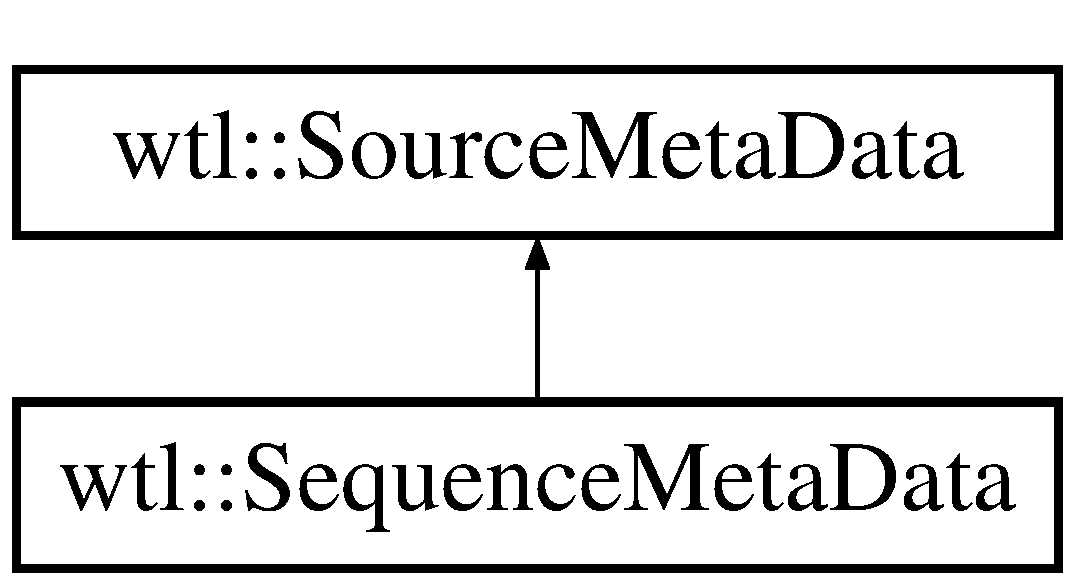
\includegraphics[height=2.000000cm]{classwtl_1_1_source_meta_data}
\end{center}
\end{figure}
\subsection*{Public Member Functions}
\begin{DoxyCompactItemize}
\item 
\hyperlink{classwtl_1_1_source_meta_data_a79f846523696923b9e7d62fab52fb96c}{Source\+Meta\+Data} ()
\item 
\hyperlink{classwtl_1_1_source_meta_data_acc7b69f117a62e3379c72584597d2d8d}{Source\+Meta\+Data} (const \hyperlink{classwtl_1_1_source_meta_data}{Source\+Meta\+Data} \&x)=default
\item 
int \hyperlink{classwtl_1_1_source_meta_data_a4053efeed2a7777d236640c94a411862}{get\+Height} () const
\begin{DoxyCompactList}\small\item\em Image Height. \end{DoxyCompactList}\item 
int \hyperlink{classwtl_1_1_source_meta_data_a42f1f73264921d73e5ba08a589630ea0}{get\+Width} () const
\begin{DoxyCompactList}\small\item\em Image Width. \end{DoxyCompactList}\item 
std\+::string \hyperlink{classwtl_1_1_source_meta_data_a2720b2135f4680d231365a3883053e13}{get\+Resolution} () const
\begin{DoxyCompactList}\small\item\em Image Resolution. \end{DoxyCompactList}\item 
std\+::string \hyperlink{classwtl_1_1_source_meta_data_a447b4425de148173e4e098a612c35b49}{get\+Source\+Name} () const
\begin{DoxyCompactList}\small\item\em Image Name. \end{DoxyCompactList}\item 
std\+::string \hyperlink{classwtl_1_1_source_meta_data_a97c4d177a47b1dc7e761e4eb652ff663}{get\+Source\+Path} () const
\begin{DoxyCompactList}\small\item\em Image Path. \end{DoxyCompactList}\item 
std\+::string \hyperlink{classwtl_1_1_source_meta_data_a08906d8f70a1de5931be41a0e25d8564}{get\+Capture\+Time\+Exif} () const
\begin{DoxyCompactList}\small\item\em Unix timestamp of an image saved in exif. \end{DoxyCompactList}\item 
unsigned \hyperlink{classwtl_1_1_source_meta_data_ac0a710c790df3e6c20a2e5e0d09a72be}{get\+Capture\+Time} () const
\begin{DoxyCompactList}\small\item\em Unix timestamp of an imag. \end{DoxyCompactList}\item 
std\+::string \hyperlink{classwtl_1_1_source_meta_data_a2f5e624ff2afb463c7833857674e6c72}{get\+Camera\+Serial\+Number} () const
\begin{DoxyCompactList}\small\item\em Serial number of camera that captured the image. \end{DoxyCompactList}\item 
std\+::string \hyperlink{classwtl_1_1_source_meta_data_aba6ebedd1aea262d0bd153ed269798c2}{get\+Camera\+Manufacturer} () const
\begin{DoxyCompactList}\small\item\em Manufacturer of camera that captured the image. \end{DoxyCompactList}\item 
std\+::string \hyperlink{classwtl_1_1_source_meta_data_a5f6e561825f34c91e81fbfa3bc036b7d}{get\+Camera\+Artn} () const
\begin{DoxyCompactList}\small\item\em Article number of camera that captured the image. \end{DoxyCompactList}\item 
std\+::string \hyperlink{classwtl_1_1_source_meta_data_a897edcd3c9426dc80d42905636c3d87d}{get\+Camera\+F\+W\+Version} () const
\begin{DoxyCompactList}\small\item\em Get Camera Firmware Version. \end{DoxyCompactList}\item 
std\+::string \hyperlink{classwtl_1_1_source_meta_data_a0743539c60ee8f8e3ece43e9404a05a4}{get\+Camera\+Name} () const
\begin{DoxyCompactList}\small\item\em Camera model name. \end{DoxyCompactList}\item 
const \hyperlink{classwtl_1_1_g_p_s_info}{G\+P\+S\+Info} \& \hyperlink{classwtl_1_1_source_meta_data_a52c2ee24703bedb5655f50652ed0b5e3}{get\+G\+P\+S\+Info} () const
\begin{DoxyCompactList}\small\item\em Get information about location of an image. \end{DoxyCompactList}\item 
\hyperlink{classwtl_1_1_g_p_s_info}{G\+P\+S\+Info} \& \hyperlink{classwtl_1_1_source_meta_data_a7b98944eaf50b06c4065ede57e13342e}{get\+G\+P\+S\+Info} ()
\begin{DoxyCompactList}\small\item\em Get information about location of an image. \end{DoxyCompactList}\item 
unsigned \hyperlink{classwtl_1_1_source_meta_data_a9bd2c8d10826432cf74f8d1f25c9edaa}{get\+Flight\+Time} () const
\begin{DoxyCompactList}\small\item\em get\+Flight\+Time \end{DoxyCompactList}\item 
double \hyperlink{classwtl_1_1_source_meta_data_ad00e12cf26115e37d1303cb9b7dc8fd7}{get\+Gimbal\+C\+P\+U\+Temp} () const
\begin{DoxyCompactList}\small\item\em get\+Gimbal\+C\+P\+U\+Temp \end{DoxyCompactList}\item 
uint16\+\_\+t \hyperlink{classwtl_1_1_source_meta_data_a2e8a400c1afa29b1b910ab7fa4b8ca66}{get\+Image\+Frequency} () const
\begin{DoxyCompactList}\small\item\em get\+Image\+Frequency \end{DoxyCompactList}\item 
void \hyperlink{classwtl_1_1_source_meta_data_a8d244e35bcf262d4651aadff0cb467d0}{set\+Source\+Name} (const std\+::string \&image\+Name)
\begin{DoxyCompactList}\small\item\em Set name of an image. \end{DoxyCompactList}\item 
void \hyperlink{classwtl_1_1_source_meta_data_a5522a30a52467ae0cd124b55b5a78111}{set\+Source\+Path} (const std\+::string \&image\+Path)
\begin{DoxyCompactList}\small\item\em Set path to the image. \end{DoxyCompactList}\item 
void \hyperlink{classwtl_1_1_source_meta_data_ad05a54221a2d34c3a4f2af9d6cd92e12}{set\+Width} (int width)
\begin{DoxyCompactList}\small\item\em set\+Width \end{DoxyCompactList}\item 
void \hyperlink{classwtl_1_1_source_meta_data_af2b87e293f1a6ce5a5920752abef850f}{set\+Height} (int height)
\begin{DoxyCompactList}\small\item\em set\+Height \end{DoxyCompactList}\item 
void \hyperlink{classwtl_1_1_source_meta_data_af8903a429b9f6187c3843d4f32e18dce}{set\+Capture\+Time} (unsigned timestamp)
\begin{DoxyCompactList}\small\item\em set\+Capture\+Time \end{DoxyCompactList}\item 
void \hyperlink{classwtl_1_1_source_meta_data_a53490561664545c7d1b7223a2c6fc9c1}{set\+Camera\+Serial\+Number} (const std\+::string \&serial\+Number)
\begin{DoxyCompactList}\small\item\em set\+Camera\+Serial\+Number \end{DoxyCompactList}\item 
void \hyperlink{classwtl_1_1_source_meta_data_a9d14f13a2af810a1b055da76ad0abf3e}{set\+Camera\+Manufacturer} (const std\+::string \&camera\+Manufacturer)
\begin{DoxyCompactList}\small\item\em set\+Camera\+Manufacturer \end{DoxyCompactList}\item 
void \hyperlink{classwtl_1_1_source_meta_data_a86eb2818b26e117721323890aaf1a800}{set\+Camera\+Artn} (const std\+::string \&camera\+Model\+Name)
\begin{DoxyCompactList}\small\item\em set\+Camera\+Model\+Name \end{DoxyCompactList}\item 
void \hyperlink{classwtl_1_1_source_meta_data_a065ad8b3e7cd473f95d7891d28afcb62}{set\+Camera\+Name} (const std\+::string \&camera\+Name)
\begin{DoxyCompactList}\small\item\em get\+Camera\+Name \end{DoxyCompactList}\item 
void \hyperlink{classwtl_1_1_source_meta_data_aeb8f04e1d221954919f36178da738862}{set\+Camera\+F\+W\+Version} (const std\+::string \&camera\+FW)
\begin{DoxyCompactList}\small\item\em Set Camera Firmware Version. \end{DoxyCompactList}\item 
void \hyperlink{classwtl_1_1_source_meta_data_a361f603d20e3084820e3869e19ec8f40}{set\+Image\+Frequency} (uint16\+\_\+t img\+Freq)
\begin{DoxyCompactList}\small\item\em set\+Image\+Frequency \end{DoxyCompactList}\item 
void \hyperlink{classwtl_1_1_source_meta_data_a8db9b3b0c1e0507ba75ae2cb6f26cb96}{set\+Flight\+Time} (unsigned flight\+Time)
\begin{DoxyCompactList}\small\item\em set\+Flight\+Time \end{DoxyCompactList}\item 
void \hyperlink{classwtl_1_1_source_meta_data_a46aa7e06e6358d6e1bf5a297ce2c9621}{set\+Gimbal\+C\+P\+U\+Temp} (double temp)
\begin{DoxyCompactList}\small\item\em set\+Gimbal\+C\+P\+U\+Temp \end{DoxyCompactList}\end{DoxyCompactItemize}
\subsection*{Protected Attributes}
\begin{DoxyCompactItemize}
\item 
std\+::string \hyperlink{classwtl_1_1_source_meta_data_adb976a4739c879d6329023ffff10ec88}{m\+\_\+\+Source\+Name} \{\}
\item 
std\+::string \hyperlink{classwtl_1_1_source_meta_data_aeddfd5e6b783a06d66b1f19b4d932c03}{m\+\_\+\+Source\+Path} \{\}
\item 
std\+::string \hyperlink{classwtl_1_1_source_meta_data_afcd3f61eccdae1bdb42cd428bdf3a5ea}{m\+\_\+\+Camera\+Name} \{\}
\item 
std\+::string \hyperlink{classwtl_1_1_source_meta_data_aa4fb21498fb68acff7be512b2b452eb4}{m\+\_\+\+Camera\+Artn} \{\}
\item 
std\+::string \hyperlink{classwtl_1_1_source_meta_data_a53ecb2596fe7cf3817dbe30c973a27a3}{m\+\_\+\+Camera\+FW} \{\}
\item 
std\+::string \hyperlink{classwtl_1_1_source_meta_data_ab7de122fe4c98d6e5efc39dba7fd5981}{m\+\_\+\+Camera\+Serial} \{\}
\item 
std\+::string \hyperlink{classwtl_1_1_source_meta_data_a3db4cdd635561f6cbc01bcd3a40c1796}{m\+\_\+\+Camera\+Manufacturer} \{\}
\item 
unsigned \hyperlink{classwtl_1_1_source_meta_data_aa4b47e89e4b6223a81dc6540390ff691}{m\+\_\+\+Timestamp} \{\}
\item 
int \hyperlink{classwtl_1_1_source_meta_data_a0e08fc3eb69bccdbb6f47b627ad937c2}{m\+\_\+\+Image\+Height} \{\}
\item 
int \hyperlink{classwtl_1_1_source_meta_data_aabd51142b0510a3a412f40643afc39ac}{m\+\_\+\+Image\+Width} \{\}
\item 
\hyperlink{classwtl_1_1_g_p_s_info}{G\+P\+S\+Info} \hyperlink{classwtl_1_1_source_meta_data_a76b8450fe6b97b6939b2f8394fb9b1d0}{m\+\_\+\+Gps\+Info} \{\}
\item 
uint16\+\_\+t \hyperlink{classwtl_1_1_source_meta_data_af294c480a5d3c2424b5441ff66255ac5}{m\+\_\+\+Image\+Freq} \{\}
\item 
unsigned \hyperlink{classwtl_1_1_source_meta_data_a361e3e090d8aadb19b5706fc15b3f900}{m\+\_\+\+Flight\+Time} \{\}
\item 
double \hyperlink{classwtl_1_1_source_meta_data_a885dfbeb71a5cf9dae0c8286a98ef757}{m\+\_\+\+Gimbal\+C\+P\+U\+Temp} \{\}
\end{DoxyCompactItemize}
\subsection*{Friends}
\begin{DoxyCompactItemize}
\item 
class \hyperlink{classwtl_1_1_source_meta_data_a89f52b56f7155da8da3c26ad5feb1bcc}{F\+F\+F\+File\+Manager}
\item 
class \hyperlink{classwtl_1_1_source_meta_data_a7d99a404a557c5e4244a8c6ec26e7648}{Thermal\+File\+Manager}
\end{DoxyCompactItemize}


\subsection{Detailed Description}
Image data not related to thermal analysis. 

Class instances are used to provide user with metadata. acquired from thermogram that are not directly related to temperature calculations. 

\subsection{Constructor \& Destructor Documentation}
\mbox{\Hypertarget{classwtl_1_1_source_meta_data_a79f846523696923b9e7d62fab52fb96c}\label{classwtl_1_1_source_meta_data_a79f846523696923b9e7d62fab52fb96c}} 
\index{wtl\+::\+Source\+Meta\+Data@{wtl\+::\+Source\+Meta\+Data}!Source\+Meta\+Data@{Source\+Meta\+Data}}
\index{Source\+Meta\+Data@{Source\+Meta\+Data}!wtl\+::\+Source\+Meta\+Data@{wtl\+::\+Source\+Meta\+Data}}
\subsubsection{\texorpdfstring{Source\+Meta\+Data()}{SourceMetaData()}\hspace{0.1cm}{\footnotesize\ttfamily [1/2]}}
{\footnotesize\ttfamily wtl\+::\+Source\+Meta\+Data\+::\+Source\+Meta\+Data (\begin{DoxyParamCaption}{ }\end{DoxyParamCaption})}

\mbox{\Hypertarget{classwtl_1_1_source_meta_data_acc7b69f117a62e3379c72584597d2d8d}\label{classwtl_1_1_source_meta_data_acc7b69f117a62e3379c72584597d2d8d}} 
\index{wtl\+::\+Source\+Meta\+Data@{wtl\+::\+Source\+Meta\+Data}!Source\+Meta\+Data@{Source\+Meta\+Data}}
\index{Source\+Meta\+Data@{Source\+Meta\+Data}!wtl\+::\+Source\+Meta\+Data@{wtl\+::\+Source\+Meta\+Data}}
\subsubsection{\texorpdfstring{Source\+Meta\+Data()}{SourceMetaData()}\hspace{0.1cm}{\footnotesize\ttfamily [2/2]}}
{\footnotesize\ttfamily wtl\+::\+Source\+Meta\+Data\+::\+Source\+Meta\+Data (\begin{DoxyParamCaption}\item[{const \hyperlink{classwtl_1_1_source_meta_data}{Source\+Meta\+Data} \&}]{x }\end{DoxyParamCaption})\hspace{0.3cm}{\ttfamily [default]}}



\subsection{Member Function Documentation}
\mbox{\Hypertarget{classwtl_1_1_source_meta_data_a5f6e561825f34c91e81fbfa3bc036b7d}\label{classwtl_1_1_source_meta_data_a5f6e561825f34c91e81fbfa3bc036b7d}} 
\index{wtl\+::\+Source\+Meta\+Data@{wtl\+::\+Source\+Meta\+Data}!get\+Camera\+Artn@{get\+Camera\+Artn}}
\index{get\+Camera\+Artn@{get\+Camera\+Artn}!wtl\+::\+Source\+Meta\+Data@{wtl\+::\+Source\+Meta\+Data}}
\subsubsection{\texorpdfstring{get\+Camera\+Artn()}{getCameraArtn()}}
{\footnotesize\ttfamily std\+::string wtl\+::\+Source\+Meta\+Data\+::get\+Camera\+Artn (\begin{DoxyParamCaption}{ }\end{DoxyParamCaption}) const}



Article number of camera that captured the image. 

\begin{DoxyReturn}{Returns}
Camera article number 
\end{DoxyReturn}
\mbox{\Hypertarget{classwtl_1_1_source_meta_data_a897edcd3c9426dc80d42905636c3d87d}\label{classwtl_1_1_source_meta_data_a897edcd3c9426dc80d42905636c3d87d}} 
\index{wtl\+::\+Source\+Meta\+Data@{wtl\+::\+Source\+Meta\+Data}!get\+Camera\+F\+W\+Version@{get\+Camera\+F\+W\+Version}}
\index{get\+Camera\+F\+W\+Version@{get\+Camera\+F\+W\+Version}!wtl\+::\+Source\+Meta\+Data@{wtl\+::\+Source\+Meta\+Data}}
\subsubsection{\texorpdfstring{get\+Camera\+F\+W\+Version()}{getCameraFWVersion()}}
{\footnotesize\ttfamily std\+::string wtl\+::\+Source\+Meta\+Data\+::get\+Camera\+F\+W\+Version (\begin{DoxyParamCaption}{ }\end{DoxyParamCaption}) const}



Get Camera Firmware Version. 

\begin{DoxyReturn}{Returns}

\end{DoxyReturn}
\mbox{\Hypertarget{classwtl_1_1_source_meta_data_aba6ebedd1aea262d0bd153ed269798c2}\label{classwtl_1_1_source_meta_data_aba6ebedd1aea262d0bd153ed269798c2}} 
\index{wtl\+::\+Source\+Meta\+Data@{wtl\+::\+Source\+Meta\+Data}!get\+Camera\+Manufacturer@{get\+Camera\+Manufacturer}}
\index{get\+Camera\+Manufacturer@{get\+Camera\+Manufacturer}!wtl\+::\+Source\+Meta\+Data@{wtl\+::\+Source\+Meta\+Data}}
\subsubsection{\texorpdfstring{get\+Camera\+Manufacturer()}{getCameraManufacturer()}}
{\footnotesize\ttfamily std\+::string wtl\+::\+Source\+Meta\+Data\+::get\+Camera\+Manufacturer (\begin{DoxyParamCaption}{ }\end{DoxyParamCaption}) const}



Manufacturer of camera that captured the image. 

\begin{DoxyReturn}{Returns}
Manufacturer as string. 
\end{DoxyReturn}
\mbox{\Hypertarget{classwtl_1_1_source_meta_data_a0743539c60ee8f8e3ece43e9404a05a4}\label{classwtl_1_1_source_meta_data_a0743539c60ee8f8e3ece43e9404a05a4}} 
\index{wtl\+::\+Source\+Meta\+Data@{wtl\+::\+Source\+Meta\+Data}!get\+Camera\+Name@{get\+Camera\+Name}}
\index{get\+Camera\+Name@{get\+Camera\+Name}!wtl\+::\+Source\+Meta\+Data@{wtl\+::\+Source\+Meta\+Data}}
\subsubsection{\texorpdfstring{get\+Camera\+Name()}{getCameraName()}}
{\footnotesize\ttfamily std\+::string wtl\+::\+Source\+Meta\+Data\+::get\+Camera\+Name (\begin{DoxyParamCaption}{ }\end{DoxyParamCaption}) const}



Camera model name. 

\begin{DoxyReturn}{Returns}

\end{DoxyReturn}
\mbox{\Hypertarget{classwtl_1_1_source_meta_data_a2f5e624ff2afb463c7833857674e6c72}\label{classwtl_1_1_source_meta_data_a2f5e624ff2afb463c7833857674e6c72}} 
\index{wtl\+::\+Source\+Meta\+Data@{wtl\+::\+Source\+Meta\+Data}!get\+Camera\+Serial\+Number@{get\+Camera\+Serial\+Number}}
\index{get\+Camera\+Serial\+Number@{get\+Camera\+Serial\+Number}!wtl\+::\+Source\+Meta\+Data@{wtl\+::\+Source\+Meta\+Data}}
\subsubsection{\texorpdfstring{get\+Camera\+Serial\+Number()}{getCameraSerialNumber()}}
{\footnotesize\ttfamily std\+::string wtl\+::\+Source\+Meta\+Data\+::get\+Camera\+Serial\+Number (\begin{DoxyParamCaption}{ }\end{DoxyParamCaption}) const}



Serial number of camera that captured the image. 

\begin{DoxyReturn}{Returns}
Camera SN string. 
\end{DoxyReturn}
\mbox{\Hypertarget{classwtl_1_1_source_meta_data_ac0a710c790df3e6c20a2e5e0d09a72be}\label{classwtl_1_1_source_meta_data_ac0a710c790df3e6c20a2e5e0d09a72be}} 
\index{wtl\+::\+Source\+Meta\+Data@{wtl\+::\+Source\+Meta\+Data}!get\+Capture\+Time@{get\+Capture\+Time}}
\index{get\+Capture\+Time@{get\+Capture\+Time}!wtl\+::\+Source\+Meta\+Data@{wtl\+::\+Source\+Meta\+Data}}
\subsubsection{\texorpdfstring{get\+Capture\+Time()}{getCaptureTime()}}
{\footnotesize\ttfamily unsigned wtl\+::\+Source\+Meta\+Data\+::get\+Capture\+Time (\begin{DoxyParamCaption}{ }\end{DoxyParamCaption}) const}



Unix timestamp of an imag. 

\begin{DoxyReturn}{Returns}
Unix timestamp as uint 
\end{DoxyReturn}
\mbox{\Hypertarget{classwtl_1_1_source_meta_data_a08906d8f70a1de5931be41a0e25d8564}\label{classwtl_1_1_source_meta_data_a08906d8f70a1de5931be41a0e25d8564}} 
\index{wtl\+::\+Source\+Meta\+Data@{wtl\+::\+Source\+Meta\+Data}!get\+Capture\+Time\+Exif@{get\+Capture\+Time\+Exif}}
\index{get\+Capture\+Time\+Exif@{get\+Capture\+Time\+Exif}!wtl\+::\+Source\+Meta\+Data@{wtl\+::\+Source\+Meta\+Data}}
\subsubsection{\texorpdfstring{get\+Capture\+Time\+Exif()}{getCaptureTimeExif()}}
{\footnotesize\ttfamily std\+::string wtl\+::\+Source\+Meta\+Data\+::get\+Capture\+Time\+Exif (\begin{DoxyParamCaption}{ }\end{DoxyParamCaption}) const}



Unix timestamp of an image saved in exif. 

\begin{DoxyReturn}{Returns}
Unix timestamp as string 
\end{DoxyReturn}
\mbox{\Hypertarget{classwtl_1_1_source_meta_data_a9bd2c8d10826432cf74f8d1f25c9edaa}\label{classwtl_1_1_source_meta_data_a9bd2c8d10826432cf74f8d1f25c9edaa}} 
\index{wtl\+::\+Source\+Meta\+Data@{wtl\+::\+Source\+Meta\+Data}!get\+Flight\+Time@{get\+Flight\+Time}}
\index{get\+Flight\+Time@{get\+Flight\+Time}!wtl\+::\+Source\+Meta\+Data@{wtl\+::\+Source\+Meta\+Data}}
\subsubsection{\texorpdfstring{get\+Flight\+Time()}{getFlightTime()}}
{\footnotesize\ttfamily unsigned wtl\+::\+Source\+Meta\+Data\+::get\+Flight\+Time (\begin{DoxyParamCaption}{ }\end{DoxyParamCaption}) const}



get\+Flight\+Time 

\mbox{\Hypertarget{classwtl_1_1_source_meta_data_ad00e12cf26115e37d1303cb9b7dc8fd7}\label{classwtl_1_1_source_meta_data_ad00e12cf26115e37d1303cb9b7dc8fd7}} 
\index{wtl\+::\+Source\+Meta\+Data@{wtl\+::\+Source\+Meta\+Data}!get\+Gimbal\+C\+P\+U\+Temp@{get\+Gimbal\+C\+P\+U\+Temp}}
\index{get\+Gimbal\+C\+P\+U\+Temp@{get\+Gimbal\+C\+P\+U\+Temp}!wtl\+::\+Source\+Meta\+Data@{wtl\+::\+Source\+Meta\+Data}}
\subsubsection{\texorpdfstring{get\+Gimbal\+C\+P\+U\+Temp()}{getGimbalCPUTemp()}}
{\footnotesize\ttfamily double wtl\+::\+Source\+Meta\+Data\+::get\+Gimbal\+C\+P\+U\+Temp (\begin{DoxyParamCaption}{ }\end{DoxyParamCaption}) const}



get\+Gimbal\+C\+P\+U\+Temp 

\begin{DoxyReturn}{Returns}

\end{DoxyReturn}
\mbox{\Hypertarget{classwtl_1_1_source_meta_data_a52c2ee24703bedb5655f50652ed0b5e3}\label{classwtl_1_1_source_meta_data_a52c2ee24703bedb5655f50652ed0b5e3}} 
\index{wtl\+::\+Source\+Meta\+Data@{wtl\+::\+Source\+Meta\+Data}!get\+G\+P\+S\+Info@{get\+G\+P\+S\+Info}}
\index{get\+G\+P\+S\+Info@{get\+G\+P\+S\+Info}!wtl\+::\+Source\+Meta\+Data@{wtl\+::\+Source\+Meta\+Data}}
\subsubsection{\texorpdfstring{get\+G\+P\+S\+Info()}{getGPSInfo()}\hspace{0.1cm}{\footnotesize\ttfamily [1/2]}}
{\footnotesize\ttfamily const \hyperlink{classwtl_1_1_g_p_s_info}{G\+P\+S\+Info}\& wtl\+::\+Source\+Meta\+Data\+::get\+G\+P\+S\+Info (\begin{DoxyParamCaption}{ }\end{DoxyParamCaption}) const}



Get information about location of an image. 

\begin{DoxyReturn}{Returns}
Read-\/only gps info instance. 
\end{DoxyReturn}
\mbox{\Hypertarget{classwtl_1_1_source_meta_data_a7b98944eaf50b06c4065ede57e13342e}\label{classwtl_1_1_source_meta_data_a7b98944eaf50b06c4065ede57e13342e}} 
\index{wtl\+::\+Source\+Meta\+Data@{wtl\+::\+Source\+Meta\+Data}!get\+G\+P\+S\+Info@{get\+G\+P\+S\+Info}}
\index{get\+G\+P\+S\+Info@{get\+G\+P\+S\+Info}!wtl\+::\+Source\+Meta\+Data@{wtl\+::\+Source\+Meta\+Data}}
\subsubsection{\texorpdfstring{get\+G\+P\+S\+Info()}{getGPSInfo()}\hspace{0.1cm}{\footnotesize\ttfamily [2/2]}}
{\footnotesize\ttfamily \hyperlink{classwtl_1_1_g_p_s_info}{G\+P\+S\+Info}\& wtl\+::\+Source\+Meta\+Data\+::get\+G\+P\+S\+Info (\begin{DoxyParamCaption}{ }\end{DoxyParamCaption})}



Get information about location of an image. 

\begin{DoxyReturn}{Returns}
Modyfiable G\+PS info instance. 
\end{DoxyReturn}
\mbox{\Hypertarget{classwtl_1_1_source_meta_data_a4053efeed2a7777d236640c94a411862}\label{classwtl_1_1_source_meta_data_a4053efeed2a7777d236640c94a411862}} 
\index{wtl\+::\+Source\+Meta\+Data@{wtl\+::\+Source\+Meta\+Data}!get\+Height@{get\+Height}}
\index{get\+Height@{get\+Height}!wtl\+::\+Source\+Meta\+Data@{wtl\+::\+Source\+Meta\+Data}}
\subsubsection{\texorpdfstring{get\+Height()}{getHeight()}}
{\footnotesize\ttfamily int wtl\+::\+Source\+Meta\+Data\+::get\+Height (\begin{DoxyParamCaption}{ }\end{DoxyParamCaption}) const}



Image Height. 

\begin{DoxyReturn}{Returns}
Height in pixels. 
\end{DoxyReturn}
\mbox{\Hypertarget{classwtl_1_1_source_meta_data_a2e8a400c1afa29b1b910ab7fa4b8ca66}\label{classwtl_1_1_source_meta_data_a2e8a400c1afa29b1b910ab7fa4b8ca66}} 
\index{wtl\+::\+Source\+Meta\+Data@{wtl\+::\+Source\+Meta\+Data}!get\+Image\+Frequency@{get\+Image\+Frequency}}
\index{get\+Image\+Frequency@{get\+Image\+Frequency}!wtl\+::\+Source\+Meta\+Data@{wtl\+::\+Source\+Meta\+Data}}
\subsubsection{\texorpdfstring{get\+Image\+Frequency()}{getImageFrequency()}}
{\footnotesize\ttfamily uint16\+\_\+t wtl\+::\+Source\+Meta\+Data\+::get\+Image\+Frequency (\begin{DoxyParamCaption}{ }\end{DoxyParamCaption}) const}



get\+Image\+Frequency 

\begin{DoxyReturn}{Returns}

\end{DoxyReturn}
\mbox{\Hypertarget{classwtl_1_1_source_meta_data_a2720b2135f4680d231365a3883053e13}\label{classwtl_1_1_source_meta_data_a2720b2135f4680d231365a3883053e13}} 
\index{wtl\+::\+Source\+Meta\+Data@{wtl\+::\+Source\+Meta\+Data}!get\+Resolution@{get\+Resolution}}
\index{get\+Resolution@{get\+Resolution}!wtl\+::\+Source\+Meta\+Data@{wtl\+::\+Source\+Meta\+Data}}
\subsubsection{\texorpdfstring{get\+Resolution()}{getResolution()}}
{\footnotesize\ttfamily std\+::string wtl\+::\+Source\+Meta\+Data\+::get\+Resolution (\begin{DoxyParamCaption}{ }\end{DoxyParamCaption}) const}



Image Resolution. 

\begin{DoxyReturn}{Returns}
Image Pixel Resolution. 
\end{DoxyReturn}
\mbox{\Hypertarget{classwtl_1_1_source_meta_data_a447b4425de148173e4e098a612c35b49}\label{classwtl_1_1_source_meta_data_a447b4425de148173e4e098a612c35b49}} 
\index{wtl\+::\+Source\+Meta\+Data@{wtl\+::\+Source\+Meta\+Data}!get\+Source\+Name@{get\+Source\+Name}}
\index{get\+Source\+Name@{get\+Source\+Name}!wtl\+::\+Source\+Meta\+Data@{wtl\+::\+Source\+Meta\+Data}}
\subsubsection{\texorpdfstring{get\+Source\+Name()}{getSourceName()}}
{\footnotesize\ttfamily std\+::string wtl\+::\+Source\+Meta\+Data\+::get\+Source\+Name (\begin{DoxyParamCaption}{ }\end{DoxyParamCaption}) const}



Image Name. 

\begin{DoxyReturn}{Returns}
Image Name 
\end{DoxyReturn}
\mbox{\Hypertarget{classwtl_1_1_source_meta_data_a97c4d177a47b1dc7e761e4eb652ff663}\label{classwtl_1_1_source_meta_data_a97c4d177a47b1dc7e761e4eb652ff663}} 
\index{wtl\+::\+Source\+Meta\+Data@{wtl\+::\+Source\+Meta\+Data}!get\+Source\+Path@{get\+Source\+Path}}
\index{get\+Source\+Path@{get\+Source\+Path}!wtl\+::\+Source\+Meta\+Data@{wtl\+::\+Source\+Meta\+Data}}
\subsubsection{\texorpdfstring{get\+Source\+Path()}{getSourcePath()}}
{\footnotesize\ttfamily std\+::string wtl\+::\+Source\+Meta\+Data\+::get\+Source\+Path (\begin{DoxyParamCaption}{ }\end{DoxyParamCaption}) const}



Image Path. 

\begin{DoxyReturn}{Returns}
Image Path 
\end{DoxyReturn}
\mbox{\Hypertarget{classwtl_1_1_source_meta_data_a42f1f73264921d73e5ba08a589630ea0}\label{classwtl_1_1_source_meta_data_a42f1f73264921d73e5ba08a589630ea0}} 
\index{wtl\+::\+Source\+Meta\+Data@{wtl\+::\+Source\+Meta\+Data}!get\+Width@{get\+Width}}
\index{get\+Width@{get\+Width}!wtl\+::\+Source\+Meta\+Data@{wtl\+::\+Source\+Meta\+Data}}
\subsubsection{\texorpdfstring{get\+Width()}{getWidth()}}
{\footnotesize\ttfamily int wtl\+::\+Source\+Meta\+Data\+::get\+Width (\begin{DoxyParamCaption}{ }\end{DoxyParamCaption}) const}



Image Width. 

\begin{DoxyReturn}{Returns}
Width in pixels. 
\end{DoxyReturn}
\mbox{\Hypertarget{classwtl_1_1_source_meta_data_a86eb2818b26e117721323890aaf1a800}\label{classwtl_1_1_source_meta_data_a86eb2818b26e117721323890aaf1a800}} 
\index{wtl\+::\+Source\+Meta\+Data@{wtl\+::\+Source\+Meta\+Data}!set\+Camera\+Artn@{set\+Camera\+Artn}}
\index{set\+Camera\+Artn@{set\+Camera\+Artn}!wtl\+::\+Source\+Meta\+Data@{wtl\+::\+Source\+Meta\+Data}}
\subsubsection{\texorpdfstring{set\+Camera\+Artn()}{setCameraArtn()}}
{\footnotesize\ttfamily void wtl\+::\+Source\+Meta\+Data\+::set\+Camera\+Artn (\begin{DoxyParamCaption}\item[{const std\+::string \&}]{camera\+Model\+Name }\end{DoxyParamCaption})}



set\+Camera\+Model\+Name 


\begin{DoxyParams}{Parameters}
{\em camera\+Model\+Name} & \\
\hline
\end{DoxyParams}
\mbox{\Hypertarget{classwtl_1_1_source_meta_data_aeb8f04e1d221954919f36178da738862}\label{classwtl_1_1_source_meta_data_aeb8f04e1d221954919f36178da738862}} 
\index{wtl\+::\+Source\+Meta\+Data@{wtl\+::\+Source\+Meta\+Data}!set\+Camera\+F\+W\+Version@{set\+Camera\+F\+W\+Version}}
\index{set\+Camera\+F\+W\+Version@{set\+Camera\+F\+W\+Version}!wtl\+::\+Source\+Meta\+Data@{wtl\+::\+Source\+Meta\+Data}}
\subsubsection{\texorpdfstring{set\+Camera\+F\+W\+Version()}{setCameraFWVersion()}}
{\footnotesize\ttfamily void wtl\+::\+Source\+Meta\+Data\+::set\+Camera\+F\+W\+Version (\begin{DoxyParamCaption}\item[{const std\+::string \&}]{camera\+FW }\end{DoxyParamCaption})}



Set Camera Firmware Version. 


\begin{DoxyParams}{Parameters}
{\em camera\+FW} & \\
\hline
\end{DoxyParams}
\mbox{\Hypertarget{classwtl_1_1_source_meta_data_a9d14f13a2af810a1b055da76ad0abf3e}\label{classwtl_1_1_source_meta_data_a9d14f13a2af810a1b055da76ad0abf3e}} 
\index{wtl\+::\+Source\+Meta\+Data@{wtl\+::\+Source\+Meta\+Data}!set\+Camera\+Manufacturer@{set\+Camera\+Manufacturer}}
\index{set\+Camera\+Manufacturer@{set\+Camera\+Manufacturer}!wtl\+::\+Source\+Meta\+Data@{wtl\+::\+Source\+Meta\+Data}}
\subsubsection{\texorpdfstring{set\+Camera\+Manufacturer()}{setCameraManufacturer()}}
{\footnotesize\ttfamily void wtl\+::\+Source\+Meta\+Data\+::set\+Camera\+Manufacturer (\begin{DoxyParamCaption}\item[{const std\+::string \&}]{camera\+Manufacturer }\end{DoxyParamCaption})}



set\+Camera\+Manufacturer 


\begin{DoxyParams}{Parameters}
{\em camera\+Manufacturer} & \\
\hline
\end{DoxyParams}
\mbox{\Hypertarget{classwtl_1_1_source_meta_data_a065ad8b3e7cd473f95d7891d28afcb62}\label{classwtl_1_1_source_meta_data_a065ad8b3e7cd473f95d7891d28afcb62}} 
\index{wtl\+::\+Source\+Meta\+Data@{wtl\+::\+Source\+Meta\+Data}!set\+Camera\+Name@{set\+Camera\+Name}}
\index{set\+Camera\+Name@{set\+Camera\+Name}!wtl\+::\+Source\+Meta\+Data@{wtl\+::\+Source\+Meta\+Data}}
\subsubsection{\texorpdfstring{set\+Camera\+Name()}{setCameraName()}}
{\footnotesize\ttfamily void wtl\+::\+Source\+Meta\+Data\+::set\+Camera\+Name (\begin{DoxyParamCaption}\item[{const std\+::string \&}]{camera\+Name }\end{DoxyParamCaption})}



get\+Camera\+Name 


\begin{DoxyParams}{Parameters}
{\em camera\+Name} & \\
\hline
\end{DoxyParams}
\mbox{\Hypertarget{classwtl_1_1_source_meta_data_a53490561664545c7d1b7223a2c6fc9c1}\label{classwtl_1_1_source_meta_data_a53490561664545c7d1b7223a2c6fc9c1}} 
\index{wtl\+::\+Source\+Meta\+Data@{wtl\+::\+Source\+Meta\+Data}!set\+Camera\+Serial\+Number@{set\+Camera\+Serial\+Number}}
\index{set\+Camera\+Serial\+Number@{set\+Camera\+Serial\+Number}!wtl\+::\+Source\+Meta\+Data@{wtl\+::\+Source\+Meta\+Data}}
\subsubsection{\texorpdfstring{set\+Camera\+Serial\+Number()}{setCameraSerialNumber()}}
{\footnotesize\ttfamily void wtl\+::\+Source\+Meta\+Data\+::set\+Camera\+Serial\+Number (\begin{DoxyParamCaption}\item[{const std\+::string \&}]{serial\+Number }\end{DoxyParamCaption})}



set\+Camera\+Serial\+Number 


\begin{DoxyParams}{Parameters}
{\em serial\+Number} & \\
\hline
\end{DoxyParams}
\mbox{\Hypertarget{classwtl_1_1_source_meta_data_af8903a429b9f6187c3843d4f32e18dce}\label{classwtl_1_1_source_meta_data_af8903a429b9f6187c3843d4f32e18dce}} 
\index{wtl\+::\+Source\+Meta\+Data@{wtl\+::\+Source\+Meta\+Data}!set\+Capture\+Time@{set\+Capture\+Time}}
\index{set\+Capture\+Time@{set\+Capture\+Time}!wtl\+::\+Source\+Meta\+Data@{wtl\+::\+Source\+Meta\+Data}}
\subsubsection{\texorpdfstring{set\+Capture\+Time()}{setCaptureTime()}}
{\footnotesize\ttfamily void wtl\+::\+Source\+Meta\+Data\+::set\+Capture\+Time (\begin{DoxyParamCaption}\item[{unsigned}]{timestamp }\end{DoxyParamCaption})}



set\+Capture\+Time 


\begin{DoxyParams}{Parameters}
{\em timestamp} & \\
\hline
\end{DoxyParams}
\mbox{\Hypertarget{classwtl_1_1_source_meta_data_a8db9b3b0c1e0507ba75ae2cb6f26cb96}\label{classwtl_1_1_source_meta_data_a8db9b3b0c1e0507ba75ae2cb6f26cb96}} 
\index{wtl\+::\+Source\+Meta\+Data@{wtl\+::\+Source\+Meta\+Data}!set\+Flight\+Time@{set\+Flight\+Time}}
\index{set\+Flight\+Time@{set\+Flight\+Time}!wtl\+::\+Source\+Meta\+Data@{wtl\+::\+Source\+Meta\+Data}}
\subsubsection{\texorpdfstring{set\+Flight\+Time()}{setFlightTime()}}
{\footnotesize\ttfamily void wtl\+::\+Source\+Meta\+Data\+::set\+Flight\+Time (\begin{DoxyParamCaption}\item[{unsigned}]{flight\+Time }\end{DoxyParamCaption})}



set\+Flight\+Time 


\begin{DoxyParams}{Parameters}
{\em flight\+Time} & \\
\hline
\end{DoxyParams}
\mbox{\Hypertarget{classwtl_1_1_source_meta_data_a46aa7e06e6358d6e1bf5a297ce2c9621}\label{classwtl_1_1_source_meta_data_a46aa7e06e6358d6e1bf5a297ce2c9621}} 
\index{wtl\+::\+Source\+Meta\+Data@{wtl\+::\+Source\+Meta\+Data}!set\+Gimbal\+C\+P\+U\+Temp@{set\+Gimbal\+C\+P\+U\+Temp}}
\index{set\+Gimbal\+C\+P\+U\+Temp@{set\+Gimbal\+C\+P\+U\+Temp}!wtl\+::\+Source\+Meta\+Data@{wtl\+::\+Source\+Meta\+Data}}
\subsubsection{\texorpdfstring{set\+Gimbal\+C\+P\+U\+Temp()}{setGimbalCPUTemp()}}
{\footnotesize\ttfamily void wtl\+::\+Source\+Meta\+Data\+::set\+Gimbal\+C\+P\+U\+Temp (\begin{DoxyParamCaption}\item[{double}]{temp }\end{DoxyParamCaption})}



set\+Gimbal\+C\+P\+U\+Temp 


\begin{DoxyParams}{Parameters}
{\em temp} & \\
\hline
\end{DoxyParams}
\mbox{\Hypertarget{classwtl_1_1_source_meta_data_af2b87e293f1a6ce5a5920752abef850f}\label{classwtl_1_1_source_meta_data_af2b87e293f1a6ce5a5920752abef850f}} 
\index{wtl\+::\+Source\+Meta\+Data@{wtl\+::\+Source\+Meta\+Data}!set\+Height@{set\+Height}}
\index{set\+Height@{set\+Height}!wtl\+::\+Source\+Meta\+Data@{wtl\+::\+Source\+Meta\+Data}}
\subsubsection{\texorpdfstring{set\+Height()}{setHeight()}}
{\footnotesize\ttfamily void wtl\+::\+Source\+Meta\+Data\+::set\+Height (\begin{DoxyParamCaption}\item[{int}]{height }\end{DoxyParamCaption})}



set\+Height 


\begin{DoxyParams}{Parameters}
{\em height} & \\
\hline
\end{DoxyParams}
\mbox{\Hypertarget{classwtl_1_1_source_meta_data_a361f603d20e3084820e3869e19ec8f40}\label{classwtl_1_1_source_meta_data_a361f603d20e3084820e3869e19ec8f40}} 
\index{wtl\+::\+Source\+Meta\+Data@{wtl\+::\+Source\+Meta\+Data}!set\+Image\+Frequency@{set\+Image\+Frequency}}
\index{set\+Image\+Frequency@{set\+Image\+Frequency}!wtl\+::\+Source\+Meta\+Data@{wtl\+::\+Source\+Meta\+Data}}
\subsubsection{\texorpdfstring{set\+Image\+Frequency()}{setImageFrequency()}}
{\footnotesize\ttfamily void wtl\+::\+Source\+Meta\+Data\+::set\+Image\+Frequency (\begin{DoxyParamCaption}\item[{uint16\+\_\+t}]{img\+Freq }\end{DoxyParamCaption})}



set\+Image\+Frequency 


\begin{DoxyParams}{Parameters}
{\em img\+Freq} & \\
\hline
\end{DoxyParams}
\mbox{\Hypertarget{classwtl_1_1_source_meta_data_a8d244e35bcf262d4651aadff0cb467d0}\label{classwtl_1_1_source_meta_data_a8d244e35bcf262d4651aadff0cb467d0}} 
\index{wtl\+::\+Source\+Meta\+Data@{wtl\+::\+Source\+Meta\+Data}!set\+Source\+Name@{set\+Source\+Name}}
\index{set\+Source\+Name@{set\+Source\+Name}!wtl\+::\+Source\+Meta\+Data@{wtl\+::\+Source\+Meta\+Data}}
\subsubsection{\texorpdfstring{set\+Source\+Name()}{setSourceName()}}
{\footnotesize\ttfamily void wtl\+::\+Source\+Meta\+Data\+::set\+Source\+Name (\begin{DoxyParamCaption}\item[{const std\+::string \&}]{image\+Name }\end{DoxyParamCaption})}



Set name of an image. 


\begin{DoxyParams}[1]{Parameters}
\mbox{\tt in}  & {\em image\+Name} & new image name string. \\
\hline
\end{DoxyParams}
\mbox{\Hypertarget{classwtl_1_1_source_meta_data_a5522a30a52467ae0cd124b55b5a78111}\label{classwtl_1_1_source_meta_data_a5522a30a52467ae0cd124b55b5a78111}} 
\index{wtl\+::\+Source\+Meta\+Data@{wtl\+::\+Source\+Meta\+Data}!set\+Source\+Path@{set\+Source\+Path}}
\index{set\+Source\+Path@{set\+Source\+Path}!wtl\+::\+Source\+Meta\+Data@{wtl\+::\+Source\+Meta\+Data}}
\subsubsection{\texorpdfstring{set\+Source\+Path()}{setSourcePath()}}
{\footnotesize\ttfamily void wtl\+::\+Source\+Meta\+Data\+::set\+Source\+Path (\begin{DoxyParamCaption}\item[{const std\+::string \&}]{image\+Path }\end{DoxyParamCaption})}



Set path to the image. 


\begin{DoxyParams}[1]{Parameters}
\mbox{\tt in}  & {\em image\+Path} & new image path. \\
\hline
\end{DoxyParams}
\mbox{\Hypertarget{classwtl_1_1_source_meta_data_ad05a54221a2d34c3a4f2af9d6cd92e12}\label{classwtl_1_1_source_meta_data_ad05a54221a2d34c3a4f2af9d6cd92e12}} 
\index{wtl\+::\+Source\+Meta\+Data@{wtl\+::\+Source\+Meta\+Data}!set\+Width@{set\+Width}}
\index{set\+Width@{set\+Width}!wtl\+::\+Source\+Meta\+Data@{wtl\+::\+Source\+Meta\+Data}}
\subsubsection{\texorpdfstring{set\+Width()}{setWidth()}}
{\footnotesize\ttfamily void wtl\+::\+Source\+Meta\+Data\+::set\+Width (\begin{DoxyParamCaption}\item[{int}]{width }\end{DoxyParamCaption})}



set\+Width 


\begin{DoxyParams}{Parameters}
{\em width} & \\
\hline
\end{DoxyParams}


\subsection{Friends And Related Function Documentation}
\mbox{\Hypertarget{classwtl_1_1_source_meta_data_a89f52b56f7155da8da3c26ad5feb1bcc}\label{classwtl_1_1_source_meta_data_a89f52b56f7155da8da3c26ad5feb1bcc}} 
\index{wtl\+::\+Source\+Meta\+Data@{wtl\+::\+Source\+Meta\+Data}!F\+F\+F\+File\+Manager@{F\+F\+F\+File\+Manager}}
\index{F\+F\+F\+File\+Manager@{F\+F\+F\+File\+Manager}!wtl\+::\+Source\+Meta\+Data@{wtl\+::\+Source\+Meta\+Data}}
\subsubsection{\texorpdfstring{F\+F\+F\+File\+Manager}{FFFFileManager}}
{\footnotesize\ttfamily friend class F\+F\+F\+File\+Manager\hspace{0.3cm}{\ttfamily [friend]}}

\mbox{\Hypertarget{classwtl_1_1_source_meta_data_a7d99a404a557c5e4244a8c6ec26e7648}\label{classwtl_1_1_source_meta_data_a7d99a404a557c5e4244a8c6ec26e7648}} 
\index{wtl\+::\+Source\+Meta\+Data@{wtl\+::\+Source\+Meta\+Data}!Thermal\+File\+Manager@{Thermal\+File\+Manager}}
\index{Thermal\+File\+Manager@{Thermal\+File\+Manager}!wtl\+::\+Source\+Meta\+Data@{wtl\+::\+Source\+Meta\+Data}}
\subsubsection{\texorpdfstring{Thermal\+File\+Manager}{ThermalFileManager}}
{\footnotesize\ttfamily friend class Thermal\+File\+Manager\hspace{0.3cm}{\ttfamily [friend]}}



\subsection{Member Data Documentation}
\mbox{\Hypertarget{classwtl_1_1_source_meta_data_aa4fb21498fb68acff7be512b2b452eb4}\label{classwtl_1_1_source_meta_data_aa4fb21498fb68acff7be512b2b452eb4}} 
\index{wtl\+::\+Source\+Meta\+Data@{wtl\+::\+Source\+Meta\+Data}!m\+\_\+\+Camera\+Artn@{m\+\_\+\+Camera\+Artn}}
\index{m\+\_\+\+Camera\+Artn@{m\+\_\+\+Camera\+Artn}!wtl\+::\+Source\+Meta\+Data@{wtl\+::\+Source\+Meta\+Data}}
\subsubsection{\texorpdfstring{m\+\_\+\+Camera\+Artn}{m\_CameraArtn}}
{\footnotesize\ttfamily std\+::string wtl\+::\+Source\+Meta\+Data\+::m\+\_\+\+Camera\+Artn \{\}\hspace{0.3cm}{\ttfamily [protected]}}

\mbox{\Hypertarget{classwtl_1_1_source_meta_data_a53ecb2596fe7cf3817dbe30c973a27a3}\label{classwtl_1_1_source_meta_data_a53ecb2596fe7cf3817dbe30c973a27a3}} 
\index{wtl\+::\+Source\+Meta\+Data@{wtl\+::\+Source\+Meta\+Data}!m\+\_\+\+Camera\+FW@{m\+\_\+\+Camera\+FW}}
\index{m\+\_\+\+Camera\+FW@{m\+\_\+\+Camera\+FW}!wtl\+::\+Source\+Meta\+Data@{wtl\+::\+Source\+Meta\+Data}}
\subsubsection{\texorpdfstring{m\+\_\+\+Camera\+FW}{m\_CameraFW}}
{\footnotesize\ttfamily std\+::string wtl\+::\+Source\+Meta\+Data\+::m\+\_\+\+Camera\+FW \{\}\hspace{0.3cm}{\ttfamily [protected]}}

\mbox{\Hypertarget{classwtl_1_1_source_meta_data_a3db4cdd635561f6cbc01bcd3a40c1796}\label{classwtl_1_1_source_meta_data_a3db4cdd635561f6cbc01bcd3a40c1796}} 
\index{wtl\+::\+Source\+Meta\+Data@{wtl\+::\+Source\+Meta\+Data}!m\+\_\+\+Camera\+Manufacturer@{m\+\_\+\+Camera\+Manufacturer}}
\index{m\+\_\+\+Camera\+Manufacturer@{m\+\_\+\+Camera\+Manufacturer}!wtl\+::\+Source\+Meta\+Data@{wtl\+::\+Source\+Meta\+Data}}
\subsubsection{\texorpdfstring{m\+\_\+\+Camera\+Manufacturer}{m\_CameraManufacturer}}
{\footnotesize\ttfamily std\+::string wtl\+::\+Source\+Meta\+Data\+::m\+\_\+\+Camera\+Manufacturer \{\}\hspace{0.3cm}{\ttfamily [protected]}}

\mbox{\Hypertarget{classwtl_1_1_source_meta_data_afcd3f61eccdae1bdb42cd428bdf3a5ea}\label{classwtl_1_1_source_meta_data_afcd3f61eccdae1bdb42cd428bdf3a5ea}} 
\index{wtl\+::\+Source\+Meta\+Data@{wtl\+::\+Source\+Meta\+Data}!m\+\_\+\+Camera\+Name@{m\+\_\+\+Camera\+Name}}
\index{m\+\_\+\+Camera\+Name@{m\+\_\+\+Camera\+Name}!wtl\+::\+Source\+Meta\+Data@{wtl\+::\+Source\+Meta\+Data}}
\subsubsection{\texorpdfstring{m\+\_\+\+Camera\+Name}{m\_CameraName}}
{\footnotesize\ttfamily std\+::string wtl\+::\+Source\+Meta\+Data\+::m\+\_\+\+Camera\+Name \{\}\hspace{0.3cm}{\ttfamily [protected]}}

\mbox{\Hypertarget{classwtl_1_1_source_meta_data_ab7de122fe4c98d6e5efc39dba7fd5981}\label{classwtl_1_1_source_meta_data_ab7de122fe4c98d6e5efc39dba7fd5981}} 
\index{wtl\+::\+Source\+Meta\+Data@{wtl\+::\+Source\+Meta\+Data}!m\+\_\+\+Camera\+Serial@{m\+\_\+\+Camera\+Serial}}
\index{m\+\_\+\+Camera\+Serial@{m\+\_\+\+Camera\+Serial}!wtl\+::\+Source\+Meta\+Data@{wtl\+::\+Source\+Meta\+Data}}
\subsubsection{\texorpdfstring{m\+\_\+\+Camera\+Serial}{m\_CameraSerial}}
{\footnotesize\ttfamily std\+::string wtl\+::\+Source\+Meta\+Data\+::m\+\_\+\+Camera\+Serial \{\}\hspace{0.3cm}{\ttfamily [protected]}}

\mbox{\Hypertarget{classwtl_1_1_source_meta_data_a361e3e090d8aadb19b5706fc15b3f900}\label{classwtl_1_1_source_meta_data_a361e3e090d8aadb19b5706fc15b3f900}} 
\index{wtl\+::\+Source\+Meta\+Data@{wtl\+::\+Source\+Meta\+Data}!m\+\_\+\+Flight\+Time@{m\+\_\+\+Flight\+Time}}
\index{m\+\_\+\+Flight\+Time@{m\+\_\+\+Flight\+Time}!wtl\+::\+Source\+Meta\+Data@{wtl\+::\+Source\+Meta\+Data}}
\subsubsection{\texorpdfstring{m\+\_\+\+Flight\+Time}{m\_FlightTime}}
{\footnotesize\ttfamily unsigned wtl\+::\+Source\+Meta\+Data\+::m\+\_\+\+Flight\+Time \{\}\hspace{0.3cm}{\ttfamily [protected]}}

\mbox{\Hypertarget{classwtl_1_1_source_meta_data_a885dfbeb71a5cf9dae0c8286a98ef757}\label{classwtl_1_1_source_meta_data_a885dfbeb71a5cf9dae0c8286a98ef757}} 
\index{wtl\+::\+Source\+Meta\+Data@{wtl\+::\+Source\+Meta\+Data}!m\+\_\+\+Gimbal\+C\+P\+U\+Temp@{m\+\_\+\+Gimbal\+C\+P\+U\+Temp}}
\index{m\+\_\+\+Gimbal\+C\+P\+U\+Temp@{m\+\_\+\+Gimbal\+C\+P\+U\+Temp}!wtl\+::\+Source\+Meta\+Data@{wtl\+::\+Source\+Meta\+Data}}
\subsubsection{\texorpdfstring{m\+\_\+\+Gimbal\+C\+P\+U\+Temp}{m\_GimbalCPUTemp}}
{\footnotesize\ttfamily double wtl\+::\+Source\+Meta\+Data\+::m\+\_\+\+Gimbal\+C\+P\+U\+Temp \{\}\hspace{0.3cm}{\ttfamily [protected]}}

\mbox{\Hypertarget{classwtl_1_1_source_meta_data_a76b8450fe6b97b6939b2f8394fb9b1d0}\label{classwtl_1_1_source_meta_data_a76b8450fe6b97b6939b2f8394fb9b1d0}} 
\index{wtl\+::\+Source\+Meta\+Data@{wtl\+::\+Source\+Meta\+Data}!m\+\_\+\+Gps\+Info@{m\+\_\+\+Gps\+Info}}
\index{m\+\_\+\+Gps\+Info@{m\+\_\+\+Gps\+Info}!wtl\+::\+Source\+Meta\+Data@{wtl\+::\+Source\+Meta\+Data}}
\subsubsection{\texorpdfstring{m\+\_\+\+Gps\+Info}{m\_GpsInfo}}
{\footnotesize\ttfamily \hyperlink{classwtl_1_1_g_p_s_info}{G\+P\+S\+Info} wtl\+::\+Source\+Meta\+Data\+::m\+\_\+\+Gps\+Info \{\}\hspace{0.3cm}{\ttfamily [protected]}}

\mbox{\Hypertarget{classwtl_1_1_source_meta_data_af294c480a5d3c2424b5441ff66255ac5}\label{classwtl_1_1_source_meta_data_af294c480a5d3c2424b5441ff66255ac5}} 
\index{wtl\+::\+Source\+Meta\+Data@{wtl\+::\+Source\+Meta\+Data}!m\+\_\+\+Image\+Freq@{m\+\_\+\+Image\+Freq}}
\index{m\+\_\+\+Image\+Freq@{m\+\_\+\+Image\+Freq}!wtl\+::\+Source\+Meta\+Data@{wtl\+::\+Source\+Meta\+Data}}
\subsubsection{\texorpdfstring{m\+\_\+\+Image\+Freq}{m\_ImageFreq}}
{\footnotesize\ttfamily uint16\+\_\+t wtl\+::\+Source\+Meta\+Data\+::m\+\_\+\+Image\+Freq \{\}\hspace{0.3cm}{\ttfamily [protected]}}

\mbox{\Hypertarget{classwtl_1_1_source_meta_data_a0e08fc3eb69bccdbb6f47b627ad937c2}\label{classwtl_1_1_source_meta_data_a0e08fc3eb69bccdbb6f47b627ad937c2}} 
\index{wtl\+::\+Source\+Meta\+Data@{wtl\+::\+Source\+Meta\+Data}!m\+\_\+\+Image\+Height@{m\+\_\+\+Image\+Height}}
\index{m\+\_\+\+Image\+Height@{m\+\_\+\+Image\+Height}!wtl\+::\+Source\+Meta\+Data@{wtl\+::\+Source\+Meta\+Data}}
\subsubsection{\texorpdfstring{m\+\_\+\+Image\+Height}{m\_ImageHeight}}
{\footnotesize\ttfamily int wtl\+::\+Source\+Meta\+Data\+::m\+\_\+\+Image\+Height \{\}\hspace{0.3cm}{\ttfamily [protected]}}

\mbox{\Hypertarget{classwtl_1_1_source_meta_data_aabd51142b0510a3a412f40643afc39ac}\label{classwtl_1_1_source_meta_data_aabd51142b0510a3a412f40643afc39ac}} 
\index{wtl\+::\+Source\+Meta\+Data@{wtl\+::\+Source\+Meta\+Data}!m\+\_\+\+Image\+Width@{m\+\_\+\+Image\+Width}}
\index{m\+\_\+\+Image\+Width@{m\+\_\+\+Image\+Width}!wtl\+::\+Source\+Meta\+Data@{wtl\+::\+Source\+Meta\+Data}}
\subsubsection{\texorpdfstring{m\+\_\+\+Image\+Width}{m\_ImageWidth}}
{\footnotesize\ttfamily int wtl\+::\+Source\+Meta\+Data\+::m\+\_\+\+Image\+Width \{\}\hspace{0.3cm}{\ttfamily [protected]}}

\mbox{\Hypertarget{classwtl_1_1_source_meta_data_adb976a4739c879d6329023ffff10ec88}\label{classwtl_1_1_source_meta_data_adb976a4739c879d6329023ffff10ec88}} 
\index{wtl\+::\+Source\+Meta\+Data@{wtl\+::\+Source\+Meta\+Data}!m\+\_\+\+Source\+Name@{m\+\_\+\+Source\+Name}}
\index{m\+\_\+\+Source\+Name@{m\+\_\+\+Source\+Name}!wtl\+::\+Source\+Meta\+Data@{wtl\+::\+Source\+Meta\+Data}}
\subsubsection{\texorpdfstring{m\+\_\+\+Source\+Name}{m\_SourceName}}
{\footnotesize\ttfamily std\+::string wtl\+::\+Source\+Meta\+Data\+::m\+\_\+\+Source\+Name \{\}\hspace{0.3cm}{\ttfamily [protected]}}

\mbox{\Hypertarget{classwtl_1_1_source_meta_data_aeddfd5e6b783a06d66b1f19b4d932c03}\label{classwtl_1_1_source_meta_data_aeddfd5e6b783a06d66b1f19b4d932c03}} 
\index{wtl\+::\+Source\+Meta\+Data@{wtl\+::\+Source\+Meta\+Data}!m\+\_\+\+Source\+Path@{m\+\_\+\+Source\+Path}}
\index{m\+\_\+\+Source\+Path@{m\+\_\+\+Source\+Path}!wtl\+::\+Source\+Meta\+Data@{wtl\+::\+Source\+Meta\+Data}}
\subsubsection{\texorpdfstring{m\+\_\+\+Source\+Path}{m\_SourcePath}}
{\footnotesize\ttfamily std\+::string wtl\+::\+Source\+Meta\+Data\+::m\+\_\+\+Source\+Path \{\}\hspace{0.3cm}{\ttfamily [protected]}}

\mbox{\Hypertarget{classwtl_1_1_source_meta_data_aa4b47e89e4b6223a81dc6540390ff691}\label{classwtl_1_1_source_meta_data_aa4b47e89e4b6223a81dc6540390ff691}} 
\index{wtl\+::\+Source\+Meta\+Data@{wtl\+::\+Source\+Meta\+Data}!m\+\_\+\+Timestamp@{m\+\_\+\+Timestamp}}
\index{m\+\_\+\+Timestamp@{m\+\_\+\+Timestamp}!wtl\+::\+Source\+Meta\+Data@{wtl\+::\+Source\+Meta\+Data}}
\subsubsection{\texorpdfstring{m\+\_\+\+Timestamp}{m\_Timestamp}}
{\footnotesize\ttfamily unsigned wtl\+::\+Source\+Meta\+Data\+::m\+\_\+\+Timestamp \{\}\hspace{0.3cm}{\ttfamily [protected]}}


\hypertarget{classwtl_1_1_thermal_image}{}\section{wtl\+:\+:Thermal\+Image Class Reference}
\label{classwtl_1_1_thermal_image}\index{wtl\+::\+Thermal\+Image@{wtl\+::\+Thermal\+Image}}


Base Class for thermograms captured by all cameras.  


Inheritance diagram for wtl\+:\+:Thermal\+Image\+:\begin{figure}[H]
\begin{center}
\leavevmode
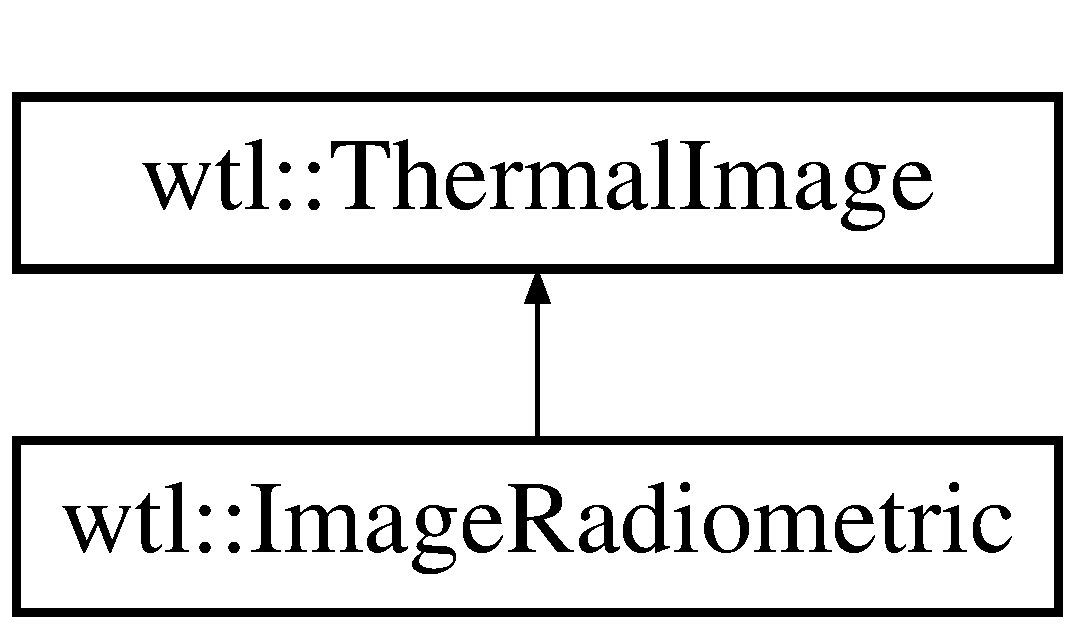
\includegraphics[height=2.000000cm]{classwtl_1_1_thermal_image}
\end{center}
\end{figure}
\subsection*{Public Member Functions}
\begin{DoxyCompactItemize}
\item 
\hyperlink{classwtl_1_1_thermal_image_ad50c00450d49151999b2cefadafc1b70}{Thermal\+Image} (const \hyperlink{classwtl_1_1_thermal_image}{Thermal\+Image} \&x)=delete
\begin{DoxyCompactList}\small\item\em Copy constructor. \end{DoxyCompactList}\item 
virtual \hyperlink{classwtl_1_1_thermal_image_a7afe55e31e0bc111a18a227cff611a35}{$\sim$\+Thermal\+Image} ()
\begin{DoxyCompactList}\small\item\em Class destructor. \end{DoxyCompactList}\item 
\hyperlink{classwtl_1_1_thermal_image}{Thermal\+Image} \& \hyperlink{classwtl_1_1_thermal_image_ac411b17ea86fd39c3737c7d9096e371c}{operator=} (const \hyperlink{classwtl_1_1_thermal_image}{Thermal\+Image} \&x)=delete
\begin{DoxyCompactList}\small\item\em Assignment operator. \end{DoxyCompactList}\item 
\hyperlink{classwtl_1_1_source_meta_data}{Source\+Meta\+Data} \& \hyperlink{classwtl_1_1_thermal_image_a3bcccd7e0d37bfb0656ec8a076379224}{get\+Image\+Meta\+Data} () const
\begin{DoxyCompactList}\small\item\em Get \hyperlink{classwtl_1_1_source_meta_data}{Source\+Meta\+Data} instance which contains non-\/temperature related data about an image. \end{DoxyCompactList}\item 
Calibration\+Parameters \& \hyperlink{classwtl_1_1_thermal_image_ad230e96412b38701538cf424074cd3e1}{get\+Image\+Calib\+Params} () const
\begin{DoxyCompactList}\small\item\em Get Calibration params instance. \end{DoxyCompactList}\item 
std\+::shared\+\_\+ptr$<$ \hyperlink{classwtl_1_1_palette}{wtl\+::\+Palette} $>$ \hyperlink{classwtl_1_1_thermal_image_a87ec0327e8fa2281caefb4ff3f67e42f}{get\+Palette} () const
\begin{DoxyCompactList}\small\item\em Get \hyperlink{classwtl_1_1_palette}{Palette}. \end{DoxyCompactList}\item 
void \hyperlink{classwtl_1_1_thermal_image_a3c53fac4f759dfdbe3f73863449326b9}{set\+Palette} (const std\+::string \&palette)
\begin{DoxyCompactList}\small\item\em Set palette to image. \end{DoxyCompactList}\item 
void \hyperlink{classwtl_1_1_thermal_image_ac72bcde5f4b324f8a0a37322ac419c82}{set\+Palette} (std\+::shared\+\_\+ptr$<$ \hyperlink{classwtl_1_1_palette}{wtl\+::\+Palette} $>$ palette)
\begin{DoxyCompactList}\small\item\em \hyperlink{classwtl_1_1_thermal_image_a3c53fac4f759dfdbe3f73863449326b9}{wtl\+::\+Thermal\+Image\+::set\+Palette} \end{DoxyCompactList}\item 
void \hyperlink{classwtl_1_1_thermal_image_aefc6b816aff2637cffb7db3ea359a365}{set\+Manual\+Range} (bool manual\+Range\+Active)
\begin{DoxyCompactList}\small\item\em Set manual range. \end{DoxyCompactList}\item 
bool \hyperlink{classwtl_1_1_thermal_image_a393678afe9b5347070219d56777546d3}{is\+Manual\+Range\+Active} ()
\begin{DoxyCompactList}\small\item\em Is Manual Range Active. \end{DoxyCompactList}\item 
bool \hyperlink{classwtl_1_1_thermal_image_aad0c616dfafb769050f434c92b50f1e7}{contains\+Visible\+Pixels} () const
\begin{DoxyCompactList}\small\item\em Digital image in visible spectrum saved in thermogram. \end{DoxyCompactList}\item 
virtual bool \hyperlink{classwtl_1_1_thermal_image_a6414e809f033c1813ac6801afcfb84b5}{is\+Radiometric\+Image} () const =0
\begin{DoxyCompactList}\small\item\em Decide whether thermal image instance contains temperature data. \end{DoxyCompactList}\item 
uint16\+\_\+t $\ast$ \hyperlink{classwtl_1_1_thermal_image_aae3499c4b035ce32972c35cbaea366eb}{get\+Visible\+Pixels} () const
\begin{DoxyCompactList}\small\item\em Get Digital image pixels in visible spectrum saved in thermogram. \end{DoxyCompactList}\item 
int \hyperlink{classwtl_1_1_thermal_image_aef736a8394a7899e696f4dcf991139ea}{get\+Image\+Size} () const
\begin{DoxyCompactList}\small\item\em Get Image size in bytes without metadata. \end{DoxyCompactList}\item 
int \hyperlink{classwtl_1_1_thermal_image_aa1a417dd0315dca5ecc14fb49e05cfc2}{get\+Number\+Of\+Pixels} () const
\begin{DoxyCompactList}\small\item\em Total number of pixels. \end{DoxyCompactList}\item 
int \hyperlink{classwtl_1_1_thermal_image_a443379442ee5ab8894138f14376d3380}{get\+Visible\+Image\+Size} () const
\item 
virtual void \hyperlink{classwtl_1_1_thermal_image_ad43f8aa46870634ad5cdd5dd784046fc}{get\+Grayscale\+Array\+Representation} (uint8\+\_\+t $\ast$$\ast$image\+Data, int \&image\+Size) const =0
\begin{DoxyCompactList}\small\item\em Get array with grayscayscale representation of thermogram that can be directly used to visualize image. \end{DoxyCompactList}\item 
virtual void \hyperlink{classwtl_1_1_thermal_image_a02a4771bd8c9e571d195fe86b7b856f2}{get\+R\+G\+B\+Array\+Representation\+With\+Overlay} (uint8\+\_\+t $\ast$image\+Data, int \&image\+Size) const =0
\begin{DoxyCompactList}\small\item\em Get array with R\+GB representation of thermogram that can be directly used to visualize image. \hyperlink{classwtl_1_1_alarms}{Alarms} and measurements overlay is added to the image. \end{DoxyCompactList}\item 
virtual void \hyperlink{classwtl_1_1_thermal_image_ae19943330497206817cda3557c4a0725}{get\+R\+G\+B\+Array\+Representation} (uint8\+\_\+t $\ast$image\+Data, int \&image\+Size) const =0
\begin{DoxyCompactList}\small\item\em Get array with R\+GB representation of thermogram that can be directly used to visualize image. \end{DoxyCompactList}\item 
virtual std\+::pair$<$ int, int $>$ \hyperlink{classwtl_1_1_thermal_image_af5c649f864be43c3f0f4f9bacc047345}{get\+Max\+Pos} () const =0
\begin{DoxyCompactList}\small\item\em Get position of pixel with maximal temperature or signal. \end{DoxyCompactList}\item 
virtual std\+::pair$<$ int, int $>$ \hyperlink{classwtl_1_1_thermal_image_a9887878b3965566660ce4c434873603a}{get\+Min\+Pos} () const =0
\begin{DoxyCompactList}\small\item\em Get position of pixel with minimum temperature or signal. \end{DoxyCompactList}\end{DoxyCompactItemize}
\subsection*{Protected Member Functions}
\begin{DoxyCompactItemize}
\item 
\hyperlink{classwtl_1_1_thermal_image_a16eb537a5a29624d94d5b89086779208}{Thermal\+Image} ()
\begin{DoxyCompactList}\small\item\em Thermal Image contructor. \end{DoxyCompactList}\item 
virtual void \hyperlink{classwtl_1_1_thermal_image_a409722852e71bedce9e9599318e0bc9e}{recalc\+Min\+Max\+Range} ()=0
\end{DoxyCompactItemize}
\subsection*{Protected Attributes}
\begin{DoxyCompactItemize}
\item 
std\+::shared\+\_\+ptr$<$ \hyperlink{classwtl_1_1_source_meta_data}{Source\+Meta\+Data} $>$ \hyperlink{classwtl_1_1_thermal_image_adb568aae4a9e0d696191b0e3ba84f1be}{m\+\_\+\+Image\+Meta\+Data}
\item 
std\+::shared\+\_\+ptr$<$ Calibration\+Parameters $>$ \hyperlink{classwtl_1_1_thermal_image_aa4e40d123c320a63d0ba8b946fe5b678}{m\+\_\+\+Calibration\+Params}
\item 
std\+::shared\+\_\+ptr$<$ \hyperlink{classwtl_1_1_palette}{Palette} $>$ \hyperlink{classwtl_1_1_thermal_image_ab294739a2c2e663df6731cbe128b34b6}{m\+\_\+\+Palette}
\item 
uint16\+\_\+t $\ast$ \hyperlink{classwtl_1_1_thermal_image_a810378588a6eb5f6bc43d2da0889ac98}{m\+\_\+\+Visible\+Pixels} = nullptr
\item 
bool \hyperlink{classwtl_1_1_thermal_image_aea72403bb30eda4f38e9a982c2957038}{m\+\_\+\+Manual\+Range\+Active} = false
\end{DoxyCompactItemize}
\subsection*{Friends}
\begin{DoxyCompactItemize}
\item 
class \hyperlink{classwtl_1_1_thermal_image_a89f52b56f7155da8da3c26ad5feb1bcc}{F\+F\+F\+File\+Manager}
\end{DoxyCompactItemize}


\subsection{Detailed Description}
Base Class for thermograms captured by all cameras. 

Provides interface for extracting and saving data to thermal images. 

\subsection{Constructor \& Destructor Documentation}
\mbox{\Hypertarget{classwtl_1_1_thermal_image_a16eb537a5a29624d94d5b89086779208}\label{classwtl_1_1_thermal_image_a16eb537a5a29624d94d5b89086779208}} 
\index{wtl\+::\+Thermal\+Image@{wtl\+::\+Thermal\+Image}!Thermal\+Image@{Thermal\+Image}}
\index{Thermal\+Image@{Thermal\+Image}!wtl\+::\+Thermal\+Image@{wtl\+::\+Thermal\+Image}}
\subsubsection{\texorpdfstring{Thermal\+Image()}{ThermalImage()}\hspace{0.1cm}{\footnotesize\ttfamily [1/2]}}
{\footnotesize\ttfamily wtl\+::\+Thermal\+Image\+::\+Thermal\+Image (\begin{DoxyParamCaption}{ }\end{DoxyParamCaption})\hspace{0.3cm}{\ttfamily [protected]}}



Thermal Image contructor. 

\mbox{\Hypertarget{classwtl_1_1_thermal_image_ad50c00450d49151999b2cefadafc1b70}\label{classwtl_1_1_thermal_image_ad50c00450d49151999b2cefadafc1b70}} 
\index{wtl\+::\+Thermal\+Image@{wtl\+::\+Thermal\+Image}!Thermal\+Image@{Thermal\+Image}}
\index{Thermal\+Image@{Thermal\+Image}!wtl\+::\+Thermal\+Image@{wtl\+::\+Thermal\+Image}}
\subsubsection{\texorpdfstring{Thermal\+Image()}{ThermalImage()}\hspace{0.1cm}{\footnotesize\ttfamily [2/2]}}
{\footnotesize\ttfamily wtl\+::\+Thermal\+Image\+::\+Thermal\+Image (\begin{DoxyParamCaption}\item[{const \hyperlink{classwtl_1_1_thermal_image}{Thermal\+Image} \&}]{x }\end{DoxyParamCaption})\hspace{0.3cm}{\ttfamily [delete]}}



Copy constructor. 


\begin{DoxyParams}{Parameters}
{\em x} & Source thermal image. \\
\hline
\end{DoxyParams}
\mbox{\Hypertarget{classwtl_1_1_thermal_image_a7afe55e31e0bc111a18a227cff611a35}\label{classwtl_1_1_thermal_image_a7afe55e31e0bc111a18a227cff611a35}} 
\index{wtl\+::\+Thermal\+Image@{wtl\+::\+Thermal\+Image}!````~Thermal\+Image@{$\sim$\+Thermal\+Image}}
\index{````~Thermal\+Image@{$\sim$\+Thermal\+Image}!wtl\+::\+Thermal\+Image@{wtl\+::\+Thermal\+Image}}
\subsubsection{\texorpdfstring{$\sim$\+Thermal\+Image()}{~ThermalImage()}}
{\footnotesize\ttfamily wtl\+::\+Thermal\+Image\+::$\sim$\+Thermal\+Image (\begin{DoxyParamCaption}{ }\end{DoxyParamCaption})\hspace{0.3cm}{\ttfamily [virtual]}}



Class destructor. 



\subsection{Member Function Documentation}
\mbox{\Hypertarget{classwtl_1_1_thermal_image_aad0c616dfafb769050f434c92b50f1e7}\label{classwtl_1_1_thermal_image_aad0c616dfafb769050f434c92b50f1e7}} 
\index{wtl\+::\+Thermal\+Image@{wtl\+::\+Thermal\+Image}!contains\+Visible\+Pixels@{contains\+Visible\+Pixels}}
\index{contains\+Visible\+Pixels@{contains\+Visible\+Pixels}!wtl\+::\+Thermal\+Image@{wtl\+::\+Thermal\+Image}}
\subsubsection{\texorpdfstring{contains\+Visible\+Pixels()}{containsVisiblePixels()}}
{\footnotesize\ttfamily bool wtl\+::\+Thermal\+Image\+::contains\+Visible\+Pixels (\begin{DoxyParamCaption}{ }\end{DoxyParamCaption}) const}



Digital image in visible spectrum saved in thermogram. 

\begin{DoxyReturn}{Returns}
True if image contains visible pixels. 
\end{DoxyReturn}
\mbox{\Hypertarget{classwtl_1_1_thermal_image_ad43f8aa46870634ad5cdd5dd784046fc}\label{classwtl_1_1_thermal_image_ad43f8aa46870634ad5cdd5dd784046fc}} 
\index{wtl\+::\+Thermal\+Image@{wtl\+::\+Thermal\+Image}!get\+Grayscale\+Array\+Representation@{get\+Grayscale\+Array\+Representation}}
\index{get\+Grayscale\+Array\+Representation@{get\+Grayscale\+Array\+Representation}!wtl\+::\+Thermal\+Image@{wtl\+::\+Thermal\+Image}}
\subsubsection{\texorpdfstring{get\+Grayscale\+Array\+Representation()}{getGrayscaleArrayRepresentation()}}
{\footnotesize\ttfamily virtual void wtl\+::\+Thermal\+Image\+::get\+Grayscale\+Array\+Representation (\begin{DoxyParamCaption}\item[{uint8\+\_\+t $\ast$$\ast$}]{image\+Data,  }\item[{int \&}]{image\+Size }\end{DoxyParamCaption}) const\hspace{0.3cm}{\ttfamily [pure virtual]}}



Get array with grayscayscale representation of thermogram that can be directly used to visualize image. 


\begin{DoxyParams}[1]{Parameters}
\mbox{\tt out}  & {\em image\+Data} & Output array parameter. \\
\hline
\mbox{\tt out}  & {\em image\+Size} & Size of an array. \\
\hline
\end{DoxyParams}


Implemented in \hyperlink{classwtl_1_1_image_radiometric_a5d32b9f0e98f81d5e917e5d33625f254}{wtl\+::\+Image\+Radiometric}.

\mbox{\Hypertarget{classwtl_1_1_thermal_image_ad230e96412b38701538cf424074cd3e1}\label{classwtl_1_1_thermal_image_ad230e96412b38701538cf424074cd3e1}} 
\index{wtl\+::\+Thermal\+Image@{wtl\+::\+Thermal\+Image}!get\+Image\+Calib\+Params@{get\+Image\+Calib\+Params}}
\index{get\+Image\+Calib\+Params@{get\+Image\+Calib\+Params}!wtl\+::\+Thermal\+Image@{wtl\+::\+Thermal\+Image}}
\subsubsection{\texorpdfstring{get\+Image\+Calib\+Params()}{getImageCalibParams()}}
{\footnotesize\ttfamily wtl\+::\+Calibration\+Parameters \& wtl\+::\+Thermal\+Image\+::get\+Image\+Calib\+Params (\begin{DoxyParamCaption}{ }\end{DoxyParamCaption}) const}



Get Calibration params instance. 

\begin{DoxyReturn}{Returns}

\end{DoxyReturn}
\mbox{\Hypertarget{classwtl_1_1_thermal_image_a3bcccd7e0d37bfb0656ec8a076379224}\label{classwtl_1_1_thermal_image_a3bcccd7e0d37bfb0656ec8a076379224}} 
\index{wtl\+::\+Thermal\+Image@{wtl\+::\+Thermal\+Image}!get\+Image\+Meta\+Data@{get\+Image\+Meta\+Data}}
\index{get\+Image\+Meta\+Data@{get\+Image\+Meta\+Data}!wtl\+::\+Thermal\+Image@{wtl\+::\+Thermal\+Image}}
\subsubsection{\texorpdfstring{get\+Image\+Meta\+Data()}{getImageMetaData()}}
{\footnotesize\ttfamily \hyperlink{classwtl_1_1_source_meta_data}{wtl\+::\+Source\+Meta\+Data} \& wtl\+::\+Thermal\+Image\+::get\+Image\+Meta\+Data (\begin{DoxyParamCaption}{ }\end{DoxyParamCaption}) const}



Get \hyperlink{classwtl_1_1_source_meta_data}{Source\+Meta\+Data} instance which contains non-\/temperature related data about an image. 

\begin{DoxyReturn}{Returns}
Instance can be used to access image meta data such as resolution, location, date of capture etc. 
\end{DoxyReturn}
\mbox{\Hypertarget{classwtl_1_1_thermal_image_aef736a8394a7899e696f4dcf991139ea}\label{classwtl_1_1_thermal_image_aef736a8394a7899e696f4dcf991139ea}} 
\index{wtl\+::\+Thermal\+Image@{wtl\+::\+Thermal\+Image}!get\+Image\+Size@{get\+Image\+Size}}
\index{get\+Image\+Size@{get\+Image\+Size}!wtl\+::\+Thermal\+Image@{wtl\+::\+Thermal\+Image}}
\subsubsection{\texorpdfstring{get\+Image\+Size()}{getImageSize()}}
{\footnotesize\ttfamily int wtl\+::\+Thermal\+Image\+::get\+Image\+Size (\begin{DoxyParamCaption}{ }\end{DoxyParamCaption}) const}



Get Image size in bytes without metadata. 

Image size in bytes, heigth $\ast$ width $\ast$ bytes per pixel. \mbox{\Hypertarget{classwtl_1_1_thermal_image_af5c649f864be43c3f0f4f9bacc047345}\label{classwtl_1_1_thermal_image_af5c649f864be43c3f0f4f9bacc047345}} 
\index{wtl\+::\+Thermal\+Image@{wtl\+::\+Thermal\+Image}!get\+Max\+Pos@{get\+Max\+Pos}}
\index{get\+Max\+Pos@{get\+Max\+Pos}!wtl\+::\+Thermal\+Image@{wtl\+::\+Thermal\+Image}}
\subsubsection{\texorpdfstring{get\+Max\+Pos()}{getMaxPos()}}
{\footnotesize\ttfamily virtual std\+::pair$<$int, int$>$ wtl\+::\+Thermal\+Image\+::get\+Max\+Pos (\begin{DoxyParamCaption}{ }\end{DoxyParamCaption}) const\hspace{0.3cm}{\ttfamily [pure virtual]}}



Get position of pixel with maximal temperature or signal. 

\begin{DoxyReturn}{Returns}
Coordinates of point with maximal temperature or signal captured in an image. 
\end{DoxyReturn}


Implemented in \hyperlink{classwtl_1_1_image_radiometric_ae1bdd0fb2335a6482ff3656dd8e9f7a3}{wtl\+::\+Image\+Radiometric}.

\mbox{\Hypertarget{classwtl_1_1_thermal_image_a9887878b3965566660ce4c434873603a}\label{classwtl_1_1_thermal_image_a9887878b3965566660ce4c434873603a}} 
\index{wtl\+::\+Thermal\+Image@{wtl\+::\+Thermal\+Image}!get\+Min\+Pos@{get\+Min\+Pos}}
\index{get\+Min\+Pos@{get\+Min\+Pos}!wtl\+::\+Thermal\+Image@{wtl\+::\+Thermal\+Image}}
\subsubsection{\texorpdfstring{get\+Min\+Pos()}{getMinPos()}}
{\footnotesize\ttfamily virtual std\+::pair$<$int, int$>$ wtl\+::\+Thermal\+Image\+::get\+Min\+Pos (\begin{DoxyParamCaption}{ }\end{DoxyParamCaption}) const\hspace{0.3cm}{\ttfamily [pure virtual]}}



Get position of pixel with minimum temperature or signal. 

\begin{DoxyReturn}{Returns}
Coordinates of point with minimal temperature or signal captured in an image. 
\end{DoxyReturn}


Implemented in \hyperlink{classwtl_1_1_image_radiometric_a4f8f918914c3de913e781de02c42e846}{wtl\+::\+Image\+Radiometric}.

\mbox{\Hypertarget{classwtl_1_1_thermal_image_aa1a417dd0315dca5ecc14fb49e05cfc2}\label{classwtl_1_1_thermal_image_aa1a417dd0315dca5ecc14fb49e05cfc2}} 
\index{wtl\+::\+Thermal\+Image@{wtl\+::\+Thermal\+Image}!get\+Number\+Of\+Pixels@{get\+Number\+Of\+Pixels}}
\index{get\+Number\+Of\+Pixels@{get\+Number\+Of\+Pixels}!wtl\+::\+Thermal\+Image@{wtl\+::\+Thermal\+Image}}
\subsubsection{\texorpdfstring{get\+Number\+Of\+Pixels()}{getNumberOfPixels()}}
{\footnotesize\ttfamily int wtl\+::\+Thermal\+Image\+::get\+Number\+Of\+Pixels (\begin{DoxyParamCaption}{ }\end{DoxyParamCaption}) const}



Total number of pixels. 

\begin{DoxyReturn}{Returns}
total number of pixels of an image. 
\end{DoxyReturn}
\mbox{\Hypertarget{classwtl_1_1_thermal_image_a87ec0327e8fa2281caefb4ff3f67e42f}\label{classwtl_1_1_thermal_image_a87ec0327e8fa2281caefb4ff3f67e42f}} 
\index{wtl\+::\+Thermal\+Image@{wtl\+::\+Thermal\+Image}!get\+Palette@{get\+Palette}}
\index{get\+Palette@{get\+Palette}!wtl\+::\+Thermal\+Image@{wtl\+::\+Thermal\+Image}}
\subsubsection{\texorpdfstring{get\+Palette()}{getPalette()}}
{\footnotesize\ttfamily std\+::shared\+\_\+ptr$<$ \hyperlink{classwtl_1_1_palette}{wtl\+::\+Palette} $>$ wtl\+::\+Thermal\+Image\+::get\+Palette (\begin{DoxyParamCaption}{ }\end{DoxyParamCaption}) const}



Get \hyperlink{classwtl_1_1_palette}{Palette}. 

\begin{DoxyReturn}{Returns}
\hyperlink{classwtl_1_1_palette}{Palette} instance that contains palette colors. 
\end{DoxyReturn}
\mbox{\Hypertarget{classwtl_1_1_thermal_image_ae19943330497206817cda3557c4a0725}\label{classwtl_1_1_thermal_image_ae19943330497206817cda3557c4a0725}} 
\index{wtl\+::\+Thermal\+Image@{wtl\+::\+Thermal\+Image}!get\+R\+G\+B\+Array\+Representation@{get\+R\+G\+B\+Array\+Representation}}
\index{get\+R\+G\+B\+Array\+Representation@{get\+R\+G\+B\+Array\+Representation}!wtl\+::\+Thermal\+Image@{wtl\+::\+Thermal\+Image}}
\subsubsection{\texorpdfstring{get\+R\+G\+B\+Array\+Representation()}{getRGBArrayRepresentation()}}
{\footnotesize\ttfamily virtual void wtl\+::\+Thermal\+Image\+::get\+R\+G\+B\+Array\+Representation (\begin{DoxyParamCaption}\item[{uint8\+\_\+t $\ast$}]{image\+Data,  }\item[{int \&}]{image\+Size }\end{DoxyParamCaption}) const\hspace{0.3cm}{\ttfamily [pure virtual]}}



Get array with R\+GB representation of thermogram that can be directly used to visualize image. 

Colors of every pixel is determined by pixel temperature. Colors from current palette are used. 
\begin{DoxyParams}[1]{Parameters}
\mbox{\tt out}  & {\em image\+Data} & Output array parameter. \\
\hline
\mbox{\tt out}  & {\em image\+Size} & Size of an array. \\
\hline
\end{DoxyParams}


Implemented in \hyperlink{classwtl_1_1_image_radiometric_a53d894315e62d9a048b2888f9a63a023}{wtl\+::\+Image\+Radiometric}.

\mbox{\Hypertarget{classwtl_1_1_thermal_image_a02a4771bd8c9e571d195fe86b7b856f2}\label{classwtl_1_1_thermal_image_a02a4771bd8c9e571d195fe86b7b856f2}} 
\index{wtl\+::\+Thermal\+Image@{wtl\+::\+Thermal\+Image}!get\+R\+G\+B\+Array\+Representation\+With\+Overlay@{get\+R\+G\+B\+Array\+Representation\+With\+Overlay}}
\index{get\+R\+G\+B\+Array\+Representation\+With\+Overlay@{get\+R\+G\+B\+Array\+Representation\+With\+Overlay}!wtl\+::\+Thermal\+Image@{wtl\+::\+Thermal\+Image}}
\subsubsection{\texorpdfstring{get\+R\+G\+B\+Array\+Representation\+With\+Overlay()}{getRGBArrayRepresentationWithOverlay()}}
{\footnotesize\ttfamily virtual void wtl\+::\+Thermal\+Image\+::get\+R\+G\+B\+Array\+Representation\+With\+Overlay (\begin{DoxyParamCaption}\item[{uint8\+\_\+t $\ast$}]{image\+Data,  }\item[{int \&}]{image\+Size }\end{DoxyParamCaption}) const\hspace{0.3cm}{\ttfamily [pure virtual]}}



Get array with R\+GB representation of thermogram that can be directly used to visualize image. \hyperlink{classwtl_1_1_alarms}{Alarms} and measurements overlay is added to the image. 


\begin{DoxyParams}[1]{Parameters}
\mbox{\tt out}  & {\em image\+Data} & Output array parameter. \\
\hline
\mbox{\tt out}  & {\em image\+Size} & Size of an array. \\
\hline
\end{DoxyParams}


Implemented in \hyperlink{classwtl_1_1_image_radiometric_a98fd9036bc6d70aa5b09c50446862428}{wtl\+::\+Image\+Radiometric}.

\mbox{\Hypertarget{classwtl_1_1_thermal_image_a443379442ee5ab8894138f14376d3380}\label{classwtl_1_1_thermal_image_a443379442ee5ab8894138f14376d3380}} 
\index{wtl\+::\+Thermal\+Image@{wtl\+::\+Thermal\+Image}!get\+Visible\+Image\+Size@{get\+Visible\+Image\+Size}}
\index{get\+Visible\+Image\+Size@{get\+Visible\+Image\+Size}!wtl\+::\+Thermal\+Image@{wtl\+::\+Thermal\+Image}}
\subsubsection{\texorpdfstring{get\+Visible\+Image\+Size()}{getVisibleImageSize()}}
{\footnotesize\ttfamily int wtl\+::\+Thermal\+Image\+::get\+Visible\+Image\+Size (\begin{DoxyParamCaption}{ }\end{DoxyParamCaption}) const}

\mbox{\Hypertarget{classwtl_1_1_thermal_image_aae3499c4b035ce32972c35cbaea366eb}\label{classwtl_1_1_thermal_image_aae3499c4b035ce32972c35cbaea366eb}} 
\index{wtl\+::\+Thermal\+Image@{wtl\+::\+Thermal\+Image}!get\+Visible\+Pixels@{get\+Visible\+Pixels}}
\index{get\+Visible\+Pixels@{get\+Visible\+Pixels}!wtl\+::\+Thermal\+Image@{wtl\+::\+Thermal\+Image}}
\subsubsection{\texorpdfstring{get\+Visible\+Pixels()}{getVisiblePixels()}}
{\footnotesize\ttfamily uint16\+\_\+t $\ast$ wtl\+::\+Thermal\+Image\+::get\+Visible\+Pixels (\begin{DoxyParamCaption}{ }\end{DoxyParamCaption}) const}



Get Digital image pixels in visible spectrum saved in thermogram. 

\begin{DoxyReturn}{Returns}
1d Array of visible 3-\/channel rgb pixels. 
\end{DoxyReturn}
\mbox{\Hypertarget{classwtl_1_1_thermal_image_a393678afe9b5347070219d56777546d3}\label{classwtl_1_1_thermal_image_a393678afe9b5347070219d56777546d3}} 
\index{wtl\+::\+Thermal\+Image@{wtl\+::\+Thermal\+Image}!is\+Manual\+Range\+Active@{is\+Manual\+Range\+Active}}
\index{is\+Manual\+Range\+Active@{is\+Manual\+Range\+Active}!wtl\+::\+Thermal\+Image@{wtl\+::\+Thermal\+Image}}
\subsubsection{\texorpdfstring{is\+Manual\+Range\+Active()}{isManualRangeActive()}}
{\footnotesize\ttfamily bool wtl\+::\+Thermal\+Image\+::is\+Manual\+Range\+Active (\begin{DoxyParamCaption}{ }\end{DoxyParamCaption})}



Is Manual Range Active. 

\begin{DoxyReturn}{Returns}
manual\+Range\+Active true for activation, false for deactivation. 
\end{DoxyReturn}
\mbox{\Hypertarget{classwtl_1_1_thermal_image_a6414e809f033c1813ac6801afcfb84b5}\label{classwtl_1_1_thermal_image_a6414e809f033c1813ac6801afcfb84b5}} 
\index{wtl\+::\+Thermal\+Image@{wtl\+::\+Thermal\+Image}!is\+Radiometric\+Image@{is\+Radiometric\+Image}}
\index{is\+Radiometric\+Image@{is\+Radiometric\+Image}!wtl\+::\+Thermal\+Image@{wtl\+::\+Thermal\+Image}}
\subsubsection{\texorpdfstring{is\+Radiometric\+Image()}{isRadiometricImage()}}
{\footnotesize\ttfamily virtual bool wtl\+::\+Thermal\+Image\+::is\+Radiometric\+Image (\begin{DoxyParamCaption}{ }\end{DoxyParamCaption}) const\hspace{0.3cm}{\ttfamily [pure virtual]}}



Decide whether thermal image instance contains temperature data. 

\begin{DoxyReturn}{Returns}
True if image contains temperature for every pixel. 
\end{DoxyReturn}


Implemented in \hyperlink{classwtl_1_1_image_radiometric_a0805bd9404ae42b94f9c47c52c19d4e6}{wtl\+::\+Image\+Radiometric}.

\mbox{\Hypertarget{classwtl_1_1_thermal_image_ac411b17ea86fd39c3737c7d9096e371c}\label{classwtl_1_1_thermal_image_ac411b17ea86fd39c3737c7d9096e371c}} 
\index{wtl\+::\+Thermal\+Image@{wtl\+::\+Thermal\+Image}!operator=@{operator=}}
\index{operator=@{operator=}!wtl\+::\+Thermal\+Image@{wtl\+::\+Thermal\+Image}}
\subsubsection{\texorpdfstring{operator=()}{operator=()}}
{\footnotesize\ttfamily \hyperlink{classwtl_1_1_thermal_image}{Thermal\+Image}\& wtl\+::\+Thermal\+Image\+::operator= (\begin{DoxyParamCaption}\item[{const \hyperlink{classwtl_1_1_thermal_image}{Thermal\+Image} \&}]{x }\end{DoxyParamCaption})\hspace{0.3cm}{\ttfamily [delete]}}



Assignment operator. 


\begin{DoxyParams}{Parameters}
{\em x} & Source Thermal Image. \\
\hline
\end{DoxyParams}
\mbox{\Hypertarget{classwtl_1_1_thermal_image_a409722852e71bedce9e9599318e0bc9e}\label{classwtl_1_1_thermal_image_a409722852e71bedce9e9599318e0bc9e}} 
\index{wtl\+::\+Thermal\+Image@{wtl\+::\+Thermal\+Image}!recalc\+Min\+Max\+Range@{recalc\+Min\+Max\+Range}}
\index{recalc\+Min\+Max\+Range@{recalc\+Min\+Max\+Range}!wtl\+::\+Thermal\+Image@{wtl\+::\+Thermal\+Image}}
\subsubsection{\texorpdfstring{recalc\+Min\+Max\+Range()}{recalcMinMaxRange()}}
{\footnotesize\ttfamily virtual void wtl\+::\+Thermal\+Image\+::recalc\+Min\+Max\+Range (\begin{DoxyParamCaption}{ }\end{DoxyParamCaption})\hspace{0.3cm}{\ttfamily [protected]}, {\ttfamily [pure virtual]}}

\mbox{\Hypertarget{classwtl_1_1_thermal_image_aefc6b816aff2637cffb7db3ea359a365}\label{classwtl_1_1_thermal_image_aefc6b816aff2637cffb7db3ea359a365}} 
\index{wtl\+::\+Thermal\+Image@{wtl\+::\+Thermal\+Image}!set\+Manual\+Range@{set\+Manual\+Range}}
\index{set\+Manual\+Range@{set\+Manual\+Range}!wtl\+::\+Thermal\+Image@{wtl\+::\+Thermal\+Image}}
\subsubsection{\texorpdfstring{set\+Manual\+Range()}{setManualRange()}}
{\footnotesize\ttfamily void wtl\+::\+Thermal\+Image\+::set\+Manual\+Range (\begin{DoxyParamCaption}\item[{bool}]{manual\+Range\+Active }\end{DoxyParamCaption})}



Set manual range. 


\begin{DoxyParams}{Parameters}
{\em manual\+Range\+Active} & true for activation, false for deactivation. \\
\hline
\end{DoxyParams}
\mbox{\Hypertarget{classwtl_1_1_thermal_image_a3c53fac4f759dfdbe3f73863449326b9}\label{classwtl_1_1_thermal_image_a3c53fac4f759dfdbe3f73863449326b9}} 
\index{wtl\+::\+Thermal\+Image@{wtl\+::\+Thermal\+Image}!set\+Palette@{set\+Palette}}
\index{set\+Palette@{set\+Palette}!wtl\+::\+Thermal\+Image@{wtl\+::\+Thermal\+Image}}
\subsubsection{\texorpdfstring{set\+Palette()}{setPalette()}\hspace{0.1cm}{\footnotesize\ttfamily [1/2]}}
{\footnotesize\ttfamily void wtl\+::\+Thermal\+Image\+::set\+Palette (\begin{DoxyParamCaption}\item[{const std\+::string \&}]{palette }\end{DoxyParamCaption})}



Set palette to image. 


\begin{DoxyParams}{Parameters}
{\em palette} & One of palettes provided by S\+DK.\\
\hline
\end{DoxyParams}
Provided palettes\+: Blue\+Red, B\+W\+Iron, B\+W\+Iron1. B\+W\+Rainbow, B\+W\+Rainbow\+HC, Gradient. Gray, Iron, Iron1, Natural, Sepia, Steps, Temperature, W\+B\+R\+GB, Black\+Red, B\+W\+R\+GB, Fire, Rainbow, Rainbow\+HC. \mbox{\Hypertarget{classwtl_1_1_thermal_image_ac72bcde5f4b324f8a0a37322ac419c82}\label{classwtl_1_1_thermal_image_ac72bcde5f4b324f8a0a37322ac419c82}} 
\index{wtl\+::\+Thermal\+Image@{wtl\+::\+Thermal\+Image}!set\+Palette@{set\+Palette}}
\index{set\+Palette@{set\+Palette}!wtl\+::\+Thermal\+Image@{wtl\+::\+Thermal\+Image}}
\subsubsection{\texorpdfstring{set\+Palette()}{setPalette()}\hspace{0.1cm}{\footnotesize\ttfamily [2/2]}}
{\footnotesize\ttfamily void wtl\+::\+Thermal\+Image\+::set\+Palette (\begin{DoxyParamCaption}\item[{std\+::shared\+\_\+ptr$<$ \hyperlink{classwtl_1_1_palette}{wtl\+::\+Palette} $>$}]{palette }\end{DoxyParamCaption})}



\hyperlink{classwtl_1_1_thermal_image_a3c53fac4f759dfdbe3f73863449326b9}{wtl\+::\+Thermal\+Image\+::set\+Palette} 


\begin{DoxyParams}{Parameters}
{\em palette} & \\
\hline
\end{DoxyParams}


\subsection{Friends And Related Function Documentation}
\mbox{\Hypertarget{classwtl_1_1_thermal_image_a89f52b56f7155da8da3c26ad5feb1bcc}\label{classwtl_1_1_thermal_image_a89f52b56f7155da8da3c26ad5feb1bcc}} 
\index{wtl\+::\+Thermal\+Image@{wtl\+::\+Thermal\+Image}!F\+F\+F\+File\+Manager@{F\+F\+F\+File\+Manager}}
\index{F\+F\+F\+File\+Manager@{F\+F\+F\+File\+Manager}!wtl\+::\+Thermal\+Image@{wtl\+::\+Thermal\+Image}}
\subsubsection{\texorpdfstring{F\+F\+F\+File\+Manager}{FFFFileManager}}
{\footnotesize\ttfamily friend class F\+F\+F\+File\+Manager\hspace{0.3cm}{\ttfamily [friend]}}



\subsection{Member Data Documentation}
\mbox{\Hypertarget{classwtl_1_1_thermal_image_aa4e40d123c320a63d0ba8b946fe5b678}\label{classwtl_1_1_thermal_image_aa4e40d123c320a63d0ba8b946fe5b678}} 
\index{wtl\+::\+Thermal\+Image@{wtl\+::\+Thermal\+Image}!m\+\_\+\+Calibration\+Params@{m\+\_\+\+Calibration\+Params}}
\index{m\+\_\+\+Calibration\+Params@{m\+\_\+\+Calibration\+Params}!wtl\+::\+Thermal\+Image@{wtl\+::\+Thermal\+Image}}
\subsubsection{\texorpdfstring{m\+\_\+\+Calibration\+Params}{m\_CalibrationParams}}
{\footnotesize\ttfamily std\+::shared\+\_\+ptr$<$Calibration\+Parameters$>$ wtl\+::\+Thermal\+Image\+::m\+\_\+\+Calibration\+Params\hspace{0.3cm}{\ttfamily [protected]}}

\mbox{\Hypertarget{classwtl_1_1_thermal_image_adb568aae4a9e0d696191b0e3ba84f1be}\label{classwtl_1_1_thermal_image_adb568aae4a9e0d696191b0e3ba84f1be}} 
\index{wtl\+::\+Thermal\+Image@{wtl\+::\+Thermal\+Image}!m\+\_\+\+Image\+Meta\+Data@{m\+\_\+\+Image\+Meta\+Data}}
\index{m\+\_\+\+Image\+Meta\+Data@{m\+\_\+\+Image\+Meta\+Data}!wtl\+::\+Thermal\+Image@{wtl\+::\+Thermal\+Image}}
\subsubsection{\texorpdfstring{m\+\_\+\+Image\+Meta\+Data}{m\_ImageMetaData}}
{\footnotesize\ttfamily std\+::shared\+\_\+ptr$<$\hyperlink{classwtl_1_1_source_meta_data}{Source\+Meta\+Data}$>$ wtl\+::\+Thermal\+Image\+::m\+\_\+\+Image\+Meta\+Data\hspace{0.3cm}{\ttfamily [protected]}}

\mbox{\Hypertarget{classwtl_1_1_thermal_image_aea72403bb30eda4f38e9a982c2957038}\label{classwtl_1_1_thermal_image_aea72403bb30eda4f38e9a982c2957038}} 
\index{wtl\+::\+Thermal\+Image@{wtl\+::\+Thermal\+Image}!m\+\_\+\+Manual\+Range\+Active@{m\+\_\+\+Manual\+Range\+Active}}
\index{m\+\_\+\+Manual\+Range\+Active@{m\+\_\+\+Manual\+Range\+Active}!wtl\+::\+Thermal\+Image@{wtl\+::\+Thermal\+Image}}
\subsubsection{\texorpdfstring{m\+\_\+\+Manual\+Range\+Active}{m\_ManualRangeActive}}
{\footnotesize\ttfamily bool wtl\+::\+Thermal\+Image\+::m\+\_\+\+Manual\+Range\+Active = false\hspace{0.3cm}{\ttfamily [protected]}}

\mbox{\Hypertarget{classwtl_1_1_thermal_image_ab294739a2c2e663df6731cbe128b34b6}\label{classwtl_1_1_thermal_image_ab294739a2c2e663df6731cbe128b34b6}} 
\index{wtl\+::\+Thermal\+Image@{wtl\+::\+Thermal\+Image}!m\+\_\+\+Palette@{m\+\_\+\+Palette}}
\index{m\+\_\+\+Palette@{m\+\_\+\+Palette}!wtl\+::\+Thermal\+Image@{wtl\+::\+Thermal\+Image}}
\subsubsection{\texorpdfstring{m\+\_\+\+Palette}{m\_Palette}}
{\footnotesize\ttfamily std\+::shared\+\_\+ptr$<$\hyperlink{classwtl_1_1_palette}{Palette}$>$ wtl\+::\+Thermal\+Image\+::m\+\_\+\+Palette\hspace{0.3cm}{\ttfamily [protected]}}

\mbox{\Hypertarget{classwtl_1_1_thermal_image_a810378588a6eb5f6bc43d2da0889ac98}\label{classwtl_1_1_thermal_image_a810378588a6eb5f6bc43d2da0889ac98}} 
\index{wtl\+::\+Thermal\+Image@{wtl\+::\+Thermal\+Image}!m\+\_\+\+Visible\+Pixels@{m\+\_\+\+Visible\+Pixels}}
\index{m\+\_\+\+Visible\+Pixels@{m\+\_\+\+Visible\+Pixels}!wtl\+::\+Thermal\+Image@{wtl\+::\+Thermal\+Image}}
\subsubsection{\texorpdfstring{m\+\_\+\+Visible\+Pixels}{m\_VisiblePixels}}
{\footnotesize\ttfamily uint16\+\_\+t$\ast$ wtl\+::\+Thermal\+Image\+::m\+\_\+\+Visible\+Pixels = nullptr\hspace{0.3cm}{\ttfamily [protected]}}


\hypertarget{structwtl_1_1_thermal_parameters}{}\section{wtl\+:\+:Thermal\+Parameters Struct Reference}
\label{structwtl_1_1_thermal_parameters}\index{wtl\+::\+Thermal\+Parameters@{wtl\+::\+Thermal\+Parameters}}


Encapsulation of all the parametrs that directly influence temperature measurements.  


\subsection*{Public Member Functions}
\begin{DoxyCompactItemize}
\item 
\hyperlink{structwtl_1_1_thermal_parameters_af0b6832e344389a25396b50ac11dac21}{Thermal\+Parameters} ()
\begin{DoxyCompactList}\small\item\em \hyperlink{structwtl_1_1_thermal_parameters}{Thermal\+Parameters} contructor. \end{DoxyCompactList}\item 
\hyperlink{structwtl_1_1_thermal_parameters_a38c0ade2f399259ba8f53efb15decae2}{Thermal\+Parameters} (const \hyperlink{structwtl_1_1_thermal_parameters}{Thermal\+Parameters} \&x)
\begin{DoxyCompactList}\small\item\em Copy constructor. \end{DoxyCompactList}\item 
\hyperlink{structwtl_1_1_thermal_parameters}{Thermal\+Parameters} \& \hyperlink{structwtl_1_1_thermal_parameters_a46f24c6affb8c7f2aa1cdebebf9a80e0}{operator=} (const \hyperlink{structwtl_1_1_thermal_parameters}{Thermal\+Parameters} \&x)
\begin{DoxyCompactList}\small\item\em Assgnment operator. \end{DoxyCompactList}\item 
\hyperlink{structwtl_1_1_thermal_parameters_a618582bffc84d4aae6fec5cab0ee5bec}{$\sim$\+Thermal\+Parameters} ()
\begin{DoxyCompactList}\small\item\em Class destructor. \end{DoxyCompactList}\end{DoxyCompactItemize}
\subsection*{Public Attributes}
\begin{DoxyCompactItemize}
\item 
double \hyperlink{structwtl_1_1_thermal_parameters_ab9768a97a062f52afb865e7d7b7e62b6}{m\+\_\+\+Emissivity}
\begin{DoxyCompactList}\small\item\em Emissivity of captured object. \end{DoxyCompactList}\item 
double \hyperlink{structwtl_1_1_thermal_parameters_a90139d2cd5373a84fdfe2260f55bebe8}{m\+\_\+\+Refl\+Temp}
\begin{DoxyCompactList}\small\item\em Reflected temperature. \end{DoxyCompactList}\item 
double \hyperlink{structwtl_1_1_thermal_parameters_a275e7c262802793de600786ffe507e07}{m\+\_\+\+Atm\+Temp}
\begin{DoxyCompactList}\small\item\em Atmospheric temperature. \end{DoxyCompactList}\item 
double \hyperlink{structwtl_1_1_thermal_parameters_aa25bcd5f011cc982fbfb3fe34cf0d4d4}{m\+\_\+\+Extern\+Optic\+Temp}
\begin{DoxyCompactList}\small\item\em External Optics temperature. \end{DoxyCompactList}\item 
double \hyperlink{structwtl_1_1_thermal_parameters_a21bbd2f6974df02a6a236712d1b4930f}{m\+\_\+\+Object\+Distance}
\begin{DoxyCompactList}\small\item\em Distance to the measured object. \end{DoxyCompactList}\item 
double \hyperlink{structwtl_1_1_thermal_parameters_a621d78c25ec992e41a3965dda391b079}{m\+\_\+\+Humidity}
\begin{DoxyCompactList}\small\item\em Air relative humidity. \end{DoxyCompactList}\item 
double \hyperlink{structwtl_1_1_thermal_parameters_add8a2b39fb17ee01521ee286cf6479b4}{m\+\_\+\+Extern\+Optic\+Trans}
\begin{DoxyCompactList}\small\item\em External Optics transmission. \end{DoxyCompactList}\end{DoxyCompactItemize}
\subsection*{Friends}
\begin{DoxyCompactItemize}
\item 
class \hyperlink{structwtl_1_1_thermal_parameters_a89f52b56f7155da8da3c26ad5feb1bcc}{F\+F\+F\+File\+Manager}
\item 
class \hyperlink{structwtl_1_1_thermal_parameters_a8172a5a280dab081475c7d9f2490442c}{Thermal\+Calculation}
\end{DoxyCompactItemize}


\subsection{Detailed Description}
Encapsulation of all the parametrs that directly influence temperature measurements. 

\subsection{Constructor \& Destructor Documentation}
\mbox{\Hypertarget{structwtl_1_1_thermal_parameters_af0b6832e344389a25396b50ac11dac21}\label{structwtl_1_1_thermal_parameters_af0b6832e344389a25396b50ac11dac21}} 
\index{wtl\+::\+Thermal\+Parameters@{wtl\+::\+Thermal\+Parameters}!Thermal\+Parameters@{Thermal\+Parameters}}
\index{Thermal\+Parameters@{Thermal\+Parameters}!wtl\+::\+Thermal\+Parameters@{wtl\+::\+Thermal\+Parameters}}
\subsubsection{\texorpdfstring{Thermal\+Parameters()}{ThermalParameters()}\hspace{0.1cm}{\footnotesize\ttfamily [1/2]}}
{\footnotesize\ttfamily wtl\+::\+Thermal\+Parameters\+::\+Thermal\+Parameters (\begin{DoxyParamCaption}{ }\end{DoxyParamCaption})}



\hyperlink{structwtl_1_1_thermal_parameters}{Thermal\+Parameters} contructor. 

\mbox{\Hypertarget{structwtl_1_1_thermal_parameters_a38c0ade2f399259ba8f53efb15decae2}\label{structwtl_1_1_thermal_parameters_a38c0ade2f399259ba8f53efb15decae2}} 
\index{wtl\+::\+Thermal\+Parameters@{wtl\+::\+Thermal\+Parameters}!Thermal\+Parameters@{Thermal\+Parameters}}
\index{Thermal\+Parameters@{Thermal\+Parameters}!wtl\+::\+Thermal\+Parameters@{wtl\+::\+Thermal\+Parameters}}
\subsubsection{\texorpdfstring{Thermal\+Parameters()}{ThermalParameters()}\hspace{0.1cm}{\footnotesize\ttfamily [2/2]}}
{\footnotesize\ttfamily wtl\+::\+Thermal\+Parameters\+::\+Thermal\+Parameters (\begin{DoxyParamCaption}\item[{const \hyperlink{structwtl_1_1_thermal_parameters}{Thermal\+Parameters} \&}]{x }\end{DoxyParamCaption})}



Copy constructor. 


\begin{DoxyParams}{Parameters}
{\em x} & Source thermal parameters instance \\
\hline
\end{DoxyParams}
\mbox{\Hypertarget{structwtl_1_1_thermal_parameters_a618582bffc84d4aae6fec5cab0ee5bec}\label{structwtl_1_1_thermal_parameters_a618582bffc84d4aae6fec5cab0ee5bec}} 
\index{wtl\+::\+Thermal\+Parameters@{wtl\+::\+Thermal\+Parameters}!````~Thermal\+Parameters@{$\sim$\+Thermal\+Parameters}}
\index{````~Thermal\+Parameters@{$\sim$\+Thermal\+Parameters}!wtl\+::\+Thermal\+Parameters@{wtl\+::\+Thermal\+Parameters}}
\subsubsection{\texorpdfstring{$\sim$\+Thermal\+Parameters()}{~ThermalParameters()}}
{\footnotesize\ttfamily wtl\+::\+Thermal\+Parameters\+::$\sim$\+Thermal\+Parameters (\begin{DoxyParamCaption}{ }\end{DoxyParamCaption})}



Class destructor. 



\subsection{Member Function Documentation}
\mbox{\Hypertarget{structwtl_1_1_thermal_parameters_a46f24c6affb8c7f2aa1cdebebf9a80e0}\label{structwtl_1_1_thermal_parameters_a46f24c6affb8c7f2aa1cdebebf9a80e0}} 
\index{wtl\+::\+Thermal\+Parameters@{wtl\+::\+Thermal\+Parameters}!operator=@{operator=}}
\index{operator=@{operator=}!wtl\+::\+Thermal\+Parameters@{wtl\+::\+Thermal\+Parameters}}
\subsubsection{\texorpdfstring{operator=()}{operator=()}}
{\footnotesize\ttfamily \hyperlink{structwtl_1_1_thermal_parameters}{Thermal\+Parameters}\& wtl\+::\+Thermal\+Parameters\+::operator= (\begin{DoxyParamCaption}\item[{const \hyperlink{structwtl_1_1_thermal_parameters}{Thermal\+Parameters} \&}]{x }\end{DoxyParamCaption})}



Assgnment operator. 


\begin{DoxyParams}{Parameters}
{\em x} & Source thermal parameters instance \\
\hline
\end{DoxyParams}


\subsection{Friends And Related Function Documentation}
\mbox{\Hypertarget{structwtl_1_1_thermal_parameters_a89f52b56f7155da8da3c26ad5feb1bcc}\label{structwtl_1_1_thermal_parameters_a89f52b56f7155da8da3c26ad5feb1bcc}} 
\index{wtl\+::\+Thermal\+Parameters@{wtl\+::\+Thermal\+Parameters}!F\+F\+F\+File\+Manager@{F\+F\+F\+File\+Manager}}
\index{F\+F\+F\+File\+Manager@{F\+F\+F\+File\+Manager}!wtl\+::\+Thermal\+Parameters@{wtl\+::\+Thermal\+Parameters}}
\subsubsection{\texorpdfstring{F\+F\+F\+File\+Manager}{FFFFileManager}}
{\footnotesize\ttfamily friend class F\+F\+F\+File\+Manager\hspace{0.3cm}{\ttfamily [friend]}}

\mbox{\Hypertarget{structwtl_1_1_thermal_parameters_a8172a5a280dab081475c7d9f2490442c}\label{structwtl_1_1_thermal_parameters_a8172a5a280dab081475c7d9f2490442c}} 
\index{wtl\+::\+Thermal\+Parameters@{wtl\+::\+Thermal\+Parameters}!Thermal\+Calculation@{Thermal\+Calculation}}
\index{Thermal\+Calculation@{Thermal\+Calculation}!wtl\+::\+Thermal\+Parameters@{wtl\+::\+Thermal\+Parameters}}
\subsubsection{\texorpdfstring{Thermal\+Calculation}{ThermalCalculation}}
{\footnotesize\ttfamily friend class Thermal\+Calculation\hspace{0.3cm}{\ttfamily [friend]}}



\subsection{Member Data Documentation}
\mbox{\Hypertarget{structwtl_1_1_thermal_parameters_a275e7c262802793de600786ffe507e07}\label{structwtl_1_1_thermal_parameters_a275e7c262802793de600786ffe507e07}} 
\index{wtl\+::\+Thermal\+Parameters@{wtl\+::\+Thermal\+Parameters}!m\+\_\+\+Atm\+Temp@{m\+\_\+\+Atm\+Temp}}
\index{m\+\_\+\+Atm\+Temp@{m\+\_\+\+Atm\+Temp}!wtl\+::\+Thermal\+Parameters@{wtl\+::\+Thermal\+Parameters}}
\subsubsection{\texorpdfstring{m\+\_\+\+Atm\+Temp}{m\_AtmTemp}}
{\footnotesize\ttfamily double wtl\+::\+Thermal\+Parameters\+::m\+\_\+\+Atm\+Temp}



Atmospheric temperature. 

\mbox{\Hypertarget{structwtl_1_1_thermal_parameters_ab9768a97a062f52afb865e7d7b7e62b6}\label{structwtl_1_1_thermal_parameters_ab9768a97a062f52afb865e7d7b7e62b6}} 
\index{wtl\+::\+Thermal\+Parameters@{wtl\+::\+Thermal\+Parameters}!m\+\_\+\+Emissivity@{m\+\_\+\+Emissivity}}
\index{m\+\_\+\+Emissivity@{m\+\_\+\+Emissivity}!wtl\+::\+Thermal\+Parameters@{wtl\+::\+Thermal\+Parameters}}
\subsubsection{\texorpdfstring{m\+\_\+\+Emissivity}{m\_Emissivity}}
{\footnotesize\ttfamily double wtl\+::\+Thermal\+Parameters\+::m\+\_\+\+Emissivity}



Emissivity of captured object. 

Effectiveness in emitting energy. Defined as ratio of tradiation of object and a black body. \mbox{\Hypertarget{structwtl_1_1_thermal_parameters_aa25bcd5f011cc982fbfb3fe34cf0d4d4}\label{structwtl_1_1_thermal_parameters_aa25bcd5f011cc982fbfb3fe34cf0d4d4}} 
\index{wtl\+::\+Thermal\+Parameters@{wtl\+::\+Thermal\+Parameters}!m\+\_\+\+Extern\+Optic\+Temp@{m\+\_\+\+Extern\+Optic\+Temp}}
\index{m\+\_\+\+Extern\+Optic\+Temp@{m\+\_\+\+Extern\+Optic\+Temp}!wtl\+::\+Thermal\+Parameters@{wtl\+::\+Thermal\+Parameters}}
\subsubsection{\texorpdfstring{m\+\_\+\+Extern\+Optic\+Temp}{m\_ExternOpticTemp}}
{\footnotesize\ttfamily double wtl\+::\+Thermal\+Parameters\+::m\+\_\+\+Extern\+Optic\+Temp}



External Optics temperature. 

\mbox{\Hypertarget{structwtl_1_1_thermal_parameters_add8a2b39fb17ee01521ee286cf6479b4}\label{structwtl_1_1_thermal_parameters_add8a2b39fb17ee01521ee286cf6479b4}} 
\index{wtl\+::\+Thermal\+Parameters@{wtl\+::\+Thermal\+Parameters}!m\+\_\+\+Extern\+Optic\+Trans@{m\+\_\+\+Extern\+Optic\+Trans}}
\index{m\+\_\+\+Extern\+Optic\+Trans@{m\+\_\+\+Extern\+Optic\+Trans}!wtl\+::\+Thermal\+Parameters@{wtl\+::\+Thermal\+Parameters}}
\subsubsection{\texorpdfstring{m\+\_\+\+Extern\+Optic\+Trans}{m\_ExternOpticTrans}}
{\footnotesize\ttfamily double wtl\+::\+Thermal\+Parameters\+::m\+\_\+\+Extern\+Optic\+Trans}



External Optics transmission. 

\mbox{\Hypertarget{structwtl_1_1_thermal_parameters_a621d78c25ec992e41a3965dda391b079}\label{structwtl_1_1_thermal_parameters_a621d78c25ec992e41a3965dda391b079}} 
\index{wtl\+::\+Thermal\+Parameters@{wtl\+::\+Thermal\+Parameters}!m\+\_\+\+Humidity@{m\+\_\+\+Humidity}}
\index{m\+\_\+\+Humidity@{m\+\_\+\+Humidity}!wtl\+::\+Thermal\+Parameters@{wtl\+::\+Thermal\+Parameters}}
\subsubsection{\texorpdfstring{m\+\_\+\+Humidity}{m\_Humidity}}
{\footnotesize\ttfamily double wtl\+::\+Thermal\+Parameters\+::m\+\_\+\+Humidity}



Air relative humidity. 

\mbox{\Hypertarget{structwtl_1_1_thermal_parameters_a21bbd2f6974df02a6a236712d1b4930f}\label{structwtl_1_1_thermal_parameters_a21bbd2f6974df02a6a236712d1b4930f}} 
\index{wtl\+::\+Thermal\+Parameters@{wtl\+::\+Thermal\+Parameters}!m\+\_\+\+Object\+Distance@{m\+\_\+\+Object\+Distance}}
\index{m\+\_\+\+Object\+Distance@{m\+\_\+\+Object\+Distance}!wtl\+::\+Thermal\+Parameters@{wtl\+::\+Thermal\+Parameters}}
\subsubsection{\texorpdfstring{m\+\_\+\+Object\+Distance}{m\_ObjectDistance}}
{\footnotesize\ttfamily double wtl\+::\+Thermal\+Parameters\+::m\+\_\+\+Object\+Distance}



Distance to the measured object. 

\mbox{\Hypertarget{structwtl_1_1_thermal_parameters_a90139d2cd5373a84fdfe2260f55bebe8}\label{structwtl_1_1_thermal_parameters_a90139d2cd5373a84fdfe2260f55bebe8}} 
\index{wtl\+::\+Thermal\+Parameters@{wtl\+::\+Thermal\+Parameters}!m\+\_\+\+Refl\+Temp@{m\+\_\+\+Refl\+Temp}}
\index{m\+\_\+\+Refl\+Temp@{m\+\_\+\+Refl\+Temp}!wtl\+::\+Thermal\+Parameters@{wtl\+::\+Thermal\+Parameters}}
\subsubsection{\texorpdfstring{m\+\_\+\+Refl\+Temp}{m\_ReflTemp}}
{\footnotesize\ttfamily double wtl\+::\+Thermal\+Parameters\+::m\+\_\+\+Refl\+Temp}



Reflected temperature. 


\hypertarget{classwtl_1_1_thermal_sequence}{}\section{wtl\+:\+:Thermal\+Sequence Class Reference}
\label{classwtl_1_1_thermal_sequence}\index{wtl\+::\+Thermal\+Sequence@{wtl\+::\+Thermal\+Sequence}}


Base Class for sequences of thermograms of all file types.  


Inheritance diagram for wtl\+:\+:Thermal\+Sequence\+:\begin{figure}[H]
\begin{center}
\leavevmode
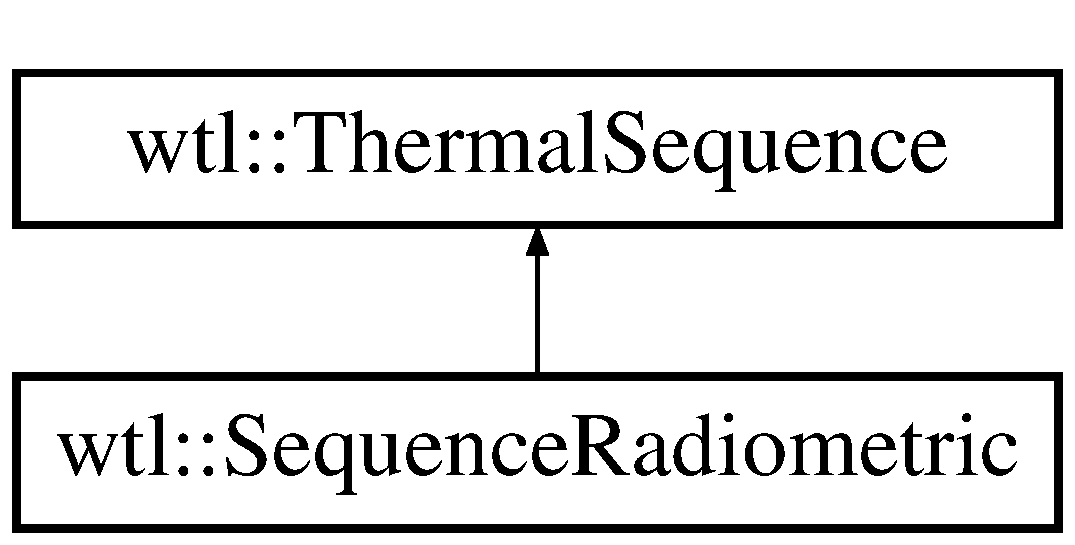
\includegraphics[height=2.000000cm]{classwtl_1_1_thermal_sequence}
\end{center}
\end{figure}
\subsection*{Public Member Functions}
\begin{DoxyCompactItemize}
\item 
virtual \hyperlink{classwtl_1_1_thermal_sequence_a51287347e2d8bfa39344d705bd720ef5}{$\sim$\+Thermal\+Sequence} ()
\begin{DoxyCompactList}\small\item\em Class destructor. \end{DoxyCompactList}\item 
\hyperlink{classwtl_1_1_thermal_sequence_a3f2298f76bddef8ad4368e412550f81d}{Thermal\+Sequence} (const \hyperlink{classwtl_1_1_thermal_sequence}{Thermal\+Sequence} \&x)=delete
\begin{DoxyCompactList}\small\item\em Copy constructor. \end{DoxyCompactList}\item 
\hyperlink{classwtl_1_1_thermal_sequence}{Thermal\+Sequence} \& \hyperlink{classwtl_1_1_thermal_sequence_a85706e752fc1fc7c1748cb2f8bedb42d}{operator=} (const \hyperlink{classwtl_1_1_thermal_sequence}{Thermal\+Sequence} \&x)=delete
\begin{DoxyCompactList}\small\item\em Assignment operator. \end{DoxyCompactList}\item 
\hyperlink{classwtl_1_1_sequence_meta_data}{Sequence\+Meta\+Data} \& \hyperlink{classwtl_1_1_thermal_sequence_a5bbbad98670f6179ce3c349fbe8e3086}{get\+Sequence\+Meta\+Data} ()
\begin{DoxyCompactList}\small\item\em Get \hyperlink{classwtl_1_1_sequence_meta_data}{Sequence\+Meta\+Data} instance which contains non-\/temperature related data about an image sequence. \end{DoxyCompactList}\item 
\hyperlink{classwtl_1_1_sequence_meta_data}{Sequence\+Meta\+Data} \& \hyperlink{classwtl_1_1_thermal_sequence_a04999d96848ef73cc7b9de708f025fa2}{get\+Sequence\+Meta\+Data} () const
\begin{DoxyCompactList}\small\item\em Get constant \hyperlink{classwtl_1_1_sequence_meta_data}{Sequence\+Meta\+Data} instance which contains non-\/temperature related data about an image sequence. \end{DoxyCompactList}\item 
virtual std\+::shared\+\_\+ptr$<$ \hyperlink{classwtl_1_1_thermal_image}{wtl\+::\+Thermal\+Image} $>$ \hyperlink{classwtl_1_1_thermal_sequence_afa7db744c4112df11b20026eae1da399}{thermal\+At} (int index) const =0
\begin{DoxyCompactList}\small\item\em Returns thermal image representation of frame at given position.\+O nly for sequences with temperature data. \end{DoxyCompactList}\item 
virtual std\+::shared\+\_\+ptr$<$ uint8\+\_\+t $>$ \hyperlink{classwtl_1_1_thermal_sequence_a0d13f29f0f89343516031c5146b62792}{get\+R\+G\+B\+Frame\+At} (int index)=0
\begin{DoxyCompactList}\small\item\em Returns 1d array with rgb representaion of frame at given position. \end{DoxyCompactList}\item 
void \hyperlink{classwtl_1_1_thermal_sequence_a47103fe0b8c101c0d2b77499f464de93}{set\+Palette} (const std\+::string \&palette)
\begin{DoxyCompactList}\small\item\em Set palette to sequence. \end{DoxyCompactList}\item 
void \hyperlink{classwtl_1_1_thermal_sequence_a5535a6cf8de61dbcf0c3d49f186c7370}{set\+Palette} (std\+::shared\+\_\+ptr$<$ \hyperlink{classwtl_1_1_palette}{wtl\+::\+Palette} $>$ palette)
\begin{DoxyCompactList}\small\item\em \hyperlink{classwtl_1_1_thermal_sequence_a47103fe0b8c101c0d2b77499f464de93}{wtl\+::\+Thermal\+Sequence\+::set\+Palette} \end{DoxyCompactList}\item 
void \hyperlink{classwtl_1_1_thermal_sequence_aedae757f2de72cee3dd3b74a5939c750}{set\+Manual\+Range} (bool manual\+Range\+Active)
\begin{DoxyCompactList}\small\item\em Set manual range. \end{DoxyCompactList}\item 
bool \hyperlink{classwtl_1_1_thermal_sequence_a7d3fb395f892aa2c040c889d2c4dc4ce}{is\+Manual\+Range\+Active} ()
\begin{DoxyCompactList}\small\item\em Is Manual Range Active. \end{DoxyCompactList}\item 
std\+::shared\+\_\+ptr$<$ \hyperlink{classwtl_1_1_palette}{wtl\+::\+Palette} $>$ \hyperlink{classwtl_1_1_thermal_sequence_a1a08643d428876f32e3155a9cd0c9f2e}{get\+Palette} () const
\item 
int \hyperlink{classwtl_1_1_thermal_sequence_a392e7c6e2b832d05c9cdb931c7cddb4f}{get\+File\+Size} ()
\begin{DoxyCompactList}\small\item\em File\+Size in bytes. \end{DoxyCompactList}\item 
virtual bool \hyperlink{classwtl_1_1_thermal_sequence_a572ec84280f0edc98c5ad0c0a0593335}{is\+Radiometric\+Sequence} () const =0
\begin{DoxyCompactList}\small\item\em Decide whether sequence is composed of thermal image instances with radiometric temperature data. \end{DoxyCompactList}\end{DoxyCompactItemize}
\subsection*{Protected Member Functions}
\begin{DoxyCompactItemize}
\item 
\hyperlink{classwtl_1_1_thermal_sequence_a222d1dcbb659a83cff8f60a431f8a370}{Thermal\+Sequence} (const std\+::string \&path, std\+::shared\+\_\+ptr$<$ wtl\+::\+F\+F\+F\+File\+Manager $>$ mngr)
\begin{DoxyCompactList}\small\item\em \hyperlink{classwtl_1_1_thermal_sequence}{Thermal\+Sequence} constructor. \end{DoxyCompactList}\item 
\hyperlink{classwtl_1_1_thermal_sequence_ae42f26a732f24d5b93182e320b360282}{Thermal\+Sequence} ()=default
\begin{DoxyCompactList}\small\item\em \hyperlink{classwtl_1_1_thermal_sequence}{Thermal\+Sequence} constructor. \end{DoxyCompactList}\end{DoxyCompactItemize}
\subsection*{Protected Attributes}
\begin{DoxyCompactItemize}
\item 
std\+::shared\+\_\+ptr$<$ \hyperlink{classwtl_1_1_sequence_meta_data}{Sequence\+Meta\+Data} $>$ \hyperlink{classwtl_1_1_thermal_sequence_a34961af460960c62b77a2d11fd49e2d3}{m\+\_\+\+Sequence\+Meta\+Data}
\item 
std\+::shared\+\_\+ptr$<$ wtl\+::\+F\+F\+F\+File\+Manager $>$ \hyperlink{classwtl_1_1_thermal_sequence_a8b3a995d93dad09344825622df9f418b}{m\+\_\+\+File\+Manager}
\item 
std\+::shared\+\_\+ptr$<$ \hyperlink{classwtl_1_1_palette}{Palette} $>$ \hyperlink{classwtl_1_1_thermal_sequence_a513c59e37dca388f0f68cbb24e527aa9}{m\+\_\+\+Palette}
\item 
bool \hyperlink{classwtl_1_1_thermal_sequence_a9af26492b66fcd91aecb62aaf1508a8f}{m\+\_\+\+Manual\+Range\+Active} = false
\end{DoxyCompactItemize}


\subsection{Detailed Description}
Base Class for sequences of thermograms of all file types. 

Provides interface for extracting and saving data to sequences of thermal images. 

\subsection{Constructor \& Destructor Documentation}
\mbox{\Hypertarget{classwtl_1_1_thermal_sequence_a222d1dcbb659a83cff8f60a431f8a370}\label{classwtl_1_1_thermal_sequence_a222d1dcbb659a83cff8f60a431f8a370}} 
\index{wtl\+::\+Thermal\+Sequence@{wtl\+::\+Thermal\+Sequence}!Thermal\+Sequence@{Thermal\+Sequence}}
\index{Thermal\+Sequence@{Thermal\+Sequence}!wtl\+::\+Thermal\+Sequence@{wtl\+::\+Thermal\+Sequence}}
\subsubsection{\texorpdfstring{Thermal\+Sequence()}{ThermalSequence()}\hspace{0.1cm}{\footnotesize\ttfamily [1/3]}}
{\footnotesize\ttfamily wtl\+::\+Thermal\+Sequence\+::\+Thermal\+Sequence (\begin{DoxyParamCaption}\item[{const std\+::string \&}]{path,  }\item[{std\+::shared\+\_\+ptr$<$ wtl\+::\+F\+F\+F\+File\+Manager $>$}]{mngr }\end{DoxyParamCaption})\hspace{0.3cm}{\ttfamily [protected]}}



\hyperlink{classwtl_1_1_thermal_sequence}{Thermal\+Sequence} constructor. 

\mbox{\Hypertarget{classwtl_1_1_thermal_sequence_ae42f26a732f24d5b93182e320b360282}\label{classwtl_1_1_thermal_sequence_ae42f26a732f24d5b93182e320b360282}} 
\index{wtl\+::\+Thermal\+Sequence@{wtl\+::\+Thermal\+Sequence}!Thermal\+Sequence@{Thermal\+Sequence}}
\index{Thermal\+Sequence@{Thermal\+Sequence}!wtl\+::\+Thermal\+Sequence@{wtl\+::\+Thermal\+Sequence}}
\subsubsection{\texorpdfstring{Thermal\+Sequence()}{ThermalSequence()}\hspace{0.1cm}{\footnotesize\ttfamily [2/3]}}
{\footnotesize\ttfamily wtl\+::\+Thermal\+Sequence\+::\+Thermal\+Sequence (\begin{DoxyParamCaption}{ }\end{DoxyParamCaption})\hspace{0.3cm}{\ttfamily [protected]}, {\ttfamily [default]}}



\hyperlink{classwtl_1_1_thermal_sequence}{Thermal\+Sequence} constructor. 

\mbox{\Hypertarget{classwtl_1_1_thermal_sequence_a51287347e2d8bfa39344d705bd720ef5}\label{classwtl_1_1_thermal_sequence_a51287347e2d8bfa39344d705bd720ef5}} 
\index{wtl\+::\+Thermal\+Sequence@{wtl\+::\+Thermal\+Sequence}!````~Thermal\+Sequence@{$\sim$\+Thermal\+Sequence}}
\index{````~Thermal\+Sequence@{$\sim$\+Thermal\+Sequence}!wtl\+::\+Thermal\+Sequence@{wtl\+::\+Thermal\+Sequence}}
\subsubsection{\texorpdfstring{$\sim$\+Thermal\+Sequence()}{~ThermalSequence()}}
{\footnotesize\ttfamily wtl\+::\+Thermal\+Sequence\+::$\sim$\+Thermal\+Sequence (\begin{DoxyParamCaption}{ }\end{DoxyParamCaption})\hspace{0.3cm}{\ttfamily [virtual]}}



Class destructor. 

\mbox{\Hypertarget{classwtl_1_1_thermal_sequence_a3f2298f76bddef8ad4368e412550f81d}\label{classwtl_1_1_thermal_sequence_a3f2298f76bddef8ad4368e412550f81d}} 
\index{wtl\+::\+Thermal\+Sequence@{wtl\+::\+Thermal\+Sequence}!Thermal\+Sequence@{Thermal\+Sequence}}
\index{Thermal\+Sequence@{Thermal\+Sequence}!wtl\+::\+Thermal\+Sequence@{wtl\+::\+Thermal\+Sequence}}
\subsubsection{\texorpdfstring{Thermal\+Sequence()}{ThermalSequence()}\hspace{0.1cm}{\footnotesize\ttfamily [3/3]}}
{\footnotesize\ttfamily wtl\+::\+Thermal\+Sequence\+::\+Thermal\+Sequence (\begin{DoxyParamCaption}\item[{const \hyperlink{classwtl_1_1_thermal_sequence}{Thermal\+Sequence} \&}]{x }\end{DoxyParamCaption})\hspace{0.3cm}{\ttfamily [delete]}}



Copy constructor. 


\begin{DoxyParams}{Parameters}
{\em x} & Source thermal sequence. \\
\hline
\end{DoxyParams}


\subsection{Member Function Documentation}
\mbox{\Hypertarget{classwtl_1_1_thermal_sequence_a392e7c6e2b832d05c9cdb931c7cddb4f}\label{classwtl_1_1_thermal_sequence_a392e7c6e2b832d05c9cdb931c7cddb4f}} 
\index{wtl\+::\+Thermal\+Sequence@{wtl\+::\+Thermal\+Sequence}!get\+File\+Size@{get\+File\+Size}}
\index{get\+File\+Size@{get\+File\+Size}!wtl\+::\+Thermal\+Sequence@{wtl\+::\+Thermal\+Sequence}}
\subsubsection{\texorpdfstring{get\+File\+Size()}{getFileSize()}}
{\footnotesize\ttfamily int wtl\+::\+Thermal\+Sequence\+::get\+File\+Size (\begin{DoxyParamCaption}{ }\end{DoxyParamCaption})}



File\+Size in bytes. 

\begin{DoxyReturn}{Returns}

\end{DoxyReturn}
\mbox{\Hypertarget{classwtl_1_1_thermal_sequence_a1a08643d428876f32e3155a9cd0c9f2e}\label{classwtl_1_1_thermal_sequence_a1a08643d428876f32e3155a9cd0c9f2e}} 
\index{wtl\+::\+Thermal\+Sequence@{wtl\+::\+Thermal\+Sequence}!get\+Palette@{get\+Palette}}
\index{get\+Palette@{get\+Palette}!wtl\+::\+Thermal\+Sequence@{wtl\+::\+Thermal\+Sequence}}
\subsubsection{\texorpdfstring{get\+Palette()}{getPalette()}}
{\footnotesize\ttfamily std\+::shared\+\_\+ptr$<$ \hyperlink{classwtl_1_1_palette}{wtl\+::\+Palette} $>$ wtl\+::\+Thermal\+Sequence\+::get\+Palette (\begin{DoxyParamCaption}{ }\end{DoxyParamCaption}) const}

\begin{DoxyReturn}{Returns}
\hyperlink{classwtl_1_1_palette}{Palette} instance that contains palette colors 

\hyperlink{classwtl_1_1_palette}{Palette} instance that contains palette colors. 
\end{DoxyReturn}
\mbox{\Hypertarget{classwtl_1_1_thermal_sequence_a0d13f29f0f89343516031c5146b62792}\label{classwtl_1_1_thermal_sequence_a0d13f29f0f89343516031c5146b62792}} 
\index{wtl\+::\+Thermal\+Sequence@{wtl\+::\+Thermal\+Sequence}!get\+R\+G\+B\+Frame\+At@{get\+R\+G\+B\+Frame\+At}}
\index{get\+R\+G\+B\+Frame\+At@{get\+R\+G\+B\+Frame\+At}!wtl\+::\+Thermal\+Sequence@{wtl\+::\+Thermal\+Sequence}}
\subsubsection{\texorpdfstring{get\+R\+G\+B\+Frame\+At()}{getRGBFrameAt()}}
{\footnotesize\ttfamily virtual std\+::shared\+\_\+ptr$<$uint8\+\_\+t$>$ wtl\+::\+Thermal\+Sequence\+::get\+R\+G\+B\+Frame\+At (\begin{DoxyParamCaption}\item[{int}]{index }\end{DoxyParamCaption})\hspace{0.3cm}{\ttfamily [pure virtual]}}



Returns 1d array with rgb representaion of frame at given position. 

Colors of every pixel is determined by pixel temperature. Colors from current palette are used. 

Implemented in \hyperlink{classwtl_1_1_sequence_radiometric_af0503fb4a89d9a356a4a68bad6da976d}{wtl\+::\+Sequence\+Radiometric}.

\mbox{\Hypertarget{classwtl_1_1_thermal_sequence_a5bbbad98670f6179ce3c349fbe8e3086}\label{classwtl_1_1_thermal_sequence_a5bbbad98670f6179ce3c349fbe8e3086}} 
\index{wtl\+::\+Thermal\+Sequence@{wtl\+::\+Thermal\+Sequence}!get\+Sequence\+Meta\+Data@{get\+Sequence\+Meta\+Data}}
\index{get\+Sequence\+Meta\+Data@{get\+Sequence\+Meta\+Data}!wtl\+::\+Thermal\+Sequence@{wtl\+::\+Thermal\+Sequence}}
\subsubsection{\texorpdfstring{get\+Sequence\+Meta\+Data()}{getSequenceMetaData()}\hspace{0.1cm}{\footnotesize\ttfamily [1/2]}}
{\footnotesize\ttfamily \hyperlink{classwtl_1_1_sequence_meta_data}{wtl\+::\+Sequence\+Meta\+Data} \& wtl\+::\+Thermal\+Sequence\+::get\+Sequence\+Meta\+Data (\begin{DoxyParamCaption}{ }\end{DoxyParamCaption})}



Get \hyperlink{classwtl_1_1_sequence_meta_data}{Sequence\+Meta\+Data} instance which contains non-\/temperature related data about an image sequence. 

\begin{DoxyReturn}{Returns}
Instance can be used to access sequence meta data such as resolution, duration, framerate etc. 
\end{DoxyReturn}
\mbox{\Hypertarget{classwtl_1_1_thermal_sequence_a04999d96848ef73cc7b9de708f025fa2}\label{classwtl_1_1_thermal_sequence_a04999d96848ef73cc7b9de708f025fa2}} 
\index{wtl\+::\+Thermal\+Sequence@{wtl\+::\+Thermal\+Sequence}!get\+Sequence\+Meta\+Data@{get\+Sequence\+Meta\+Data}}
\index{get\+Sequence\+Meta\+Data@{get\+Sequence\+Meta\+Data}!wtl\+::\+Thermal\+Sequence@{wtl\+::\+Thermal\+Sequence}}
\subsubsection{\texorpdfstring{get\+Sequence\+Meta\+Data()}{getSequenceMetaData()}\hspace{0.1cm}{\footnotesize\ttfamily [2/2]}}
{\footnotesize\ttfamily \hyperlink{classwtl_1_1_sequence_meta_data}{wtl\+::\+Sequence\+Meta\+Data} \& wtl\+::\+Thermal\+Sequence\+::get\+Sequence\+Meta\+Data (\begin{DoxyParamCaption}{ }\end{DoxyParamCaption}) const}



Get constant \hyperlink{classwtl_1_1_sequence_meta_data}{Sequence\+Meta\+Data} instance which contains non-\/temperature related data about an image sequence. 

\begin{DoxyReturn}{Returns}
Instance can be used to access sequence meta data such as resolution, duration, framerate etc. 
\end{DoxyReturn}
\mbox{\Hypertarget{classwtl_1_1_thermal_sequence_a7d3fb395f892aa2c040c889d2c4dc4ce}\label{classwtl_1_1_thermal_sequence_a7d3fb395f892aa2c040c889d2c4dc4ce}} 
\index{wtl\+::\+Thermal\+Sequence@{wtl\+::\+Thermal\+Sequence}!is\+Manual\+Range\+Active@{is\+Manual\+Range\+Active}}
\index{is\+Manual\+Range\+Active@{is\+Manual\+Range\+Active}!wtl\+::\+Thermal\+Sequence@{wtl\+::\+Thermal\+Sequence}}
\subsubsection{\texorpdfstring{is\+Manual\+Range\+Active()}{isManualRangeActive()}}
{\footnotesize\ttfamily bool wtl\+::\+Thermal\+Sequence\+::is\+Manual\+Range\+Active (\begin{DoxyParamCaption}{ }\end{DoxyParamCaption})}



Is Manual Range Active. 

\begin{DoxyReturn}{Returns}
manual\+Range\+Active true for active, false otherwise. 
\end{DoxyReturn}
\mbox{\Hypertarget{classwtl_1_1_thermal_sequence_a572ec84280f0edc98c5ad0c0a0593335}\label{classwtl_1_1_thermal_sequence_a572ec84280f0edc98c5ad0c0a0593335}} 
\index{wtl\+::\+Thermal\+Sequence@{wtl\+::\+Thermal\+Sequence}!is\+Radiometric\+Sequence@{is\+Radiometric\+Sequence}}
\index{is\+Radiometric\+Sequence@{is\+Radiometric\+Sequence}!wtl\+::\+Thermal\+Sequence@{wtl\+::\+Thermal\+Sequence}}
\subsubsection{\texorpdfstring{is\+Radiometric\+Sequence()}{isRadiometricSequence()}}
{\footnotesize\ttfamily virtual bool wtl\+::\+Thermal\+Sequence\+::is\+Radiometric\+Sequence (\begin{DoxyParamCaption}{ }\end{DoxyParamCaption}) const\hspace{0.3cm}{\ttfamily [pure virtual]}}



Decide whether sequence is composed of thermal image instances with radiometric temperature data. 

\begin{DoxyReturn}{Returns}
True if image contains temperature for every pixel 
\end{DoxyReturn}


Implemented in \hyperlink{classwtl_1_1_sequence_radiometric_aa0b063cfe218f95cd57412344d4f9a04}{wtl\+::\+Sequence\+Radiometric}.

\mbox{\Hypertarget{classwtl_1_1_thermal_sequence_a85706e752fc1fc7c1748cb2f8bedb42d}\label{classwtl_1_1_thermal_sequence_a85706e752fc1fc7c1748cb2f8bedb42d}} 
\index{wtl\+::\+Thermal\+Sequence@{wtl\+::\+Thermal\+Sequence}!operator=@{operator=}}
\index{operator=@{operator=}!wtl\+::\+Thermal\+Sequence@{wtl\+::\+Thermal\+Sequence}}
\subsubsection{\texorpdfstring{operator=()}{operator=()}}
{\footnotesize\ttfamily \hyperlink{classwtl_1_1_thermal_sequence}{Thermal\+Sequence}\& wtl\+::\+Thermal\+Sequence\+::operator= (\begin{DoxyParamCaption}\item[{const \hyperlink{classwtl_1_1_thermal_sequence}{Thermal\+Sequence} \&}]{x }\end{DoxyParamCaption})\hspace{0.3cm}{\ttfamily [delete]}}



Assignment operator. 


\begin{DoxyParams}{Parameters}
{\em x} & Source thermal sequence. \\
\hline
\end{DoxyParams}
\mbox{\Hypertarget{classwtl_1_1_thermal_sequence_aedae757f2de72cee3dd3b74a5939c750}\label{classwtl_1_1_thermal_sequence_aedae757f2de72cee3dd3b74a5939c750}} 
\index{wtl\+::\+Thermal\+Sequence@{wtl\+::\+Thermal\+Sequence}!set\+Manual\+Range@{set\+Manual\+Range}}
\index{set\+Manual\+Range@{set\+Manual\+Range}!wtl\+::\+Thermal\+Sequence@{wtl\+::\+Thermal\+Sequence}}
\subsubsection{\texorpdfstring{set\+Manual\+Range()}{setManualRange()}}
{\footnotesize\ttfamily void wtl\+::\+Thermal\+Sequence\+::set\+Manual\+Range (\begin{DoxyParamCaption}\item[{bool}]{manual\+Range\+Active }\end{DoxyParamCaption})}



Set manual range. 


\begin{DoxyParams}{Parameters}
{\em manual\+Range\+Active} & true for activation, false for deactivation. \\
\hline
\end{DoxyParams}
\mbox{\Hypertarget{classwtl_1_1_thermal_sequence_a47103fe0b8c101c0d2b77499f464de93}\label{classwtl_1_1_thermal_sequence_a47103fe0b8c101c0d2b77499f464de93}} 
\index{wtl\+::\+Thermal\+Sequence@{wtl\+::\+Thermal\+Sequence}!set\+Palette@{set\+Palette}}
\index{set\+Palette@{set\+Palette}!wtl\+::\+Thermal\+Sequence@{wtl\+::\+Thermal\+Sequence}}
\subsubsection{\texorpdfstring{set\+Palette()}{setPalette()}\hspace{0.1cm}{\footnotesize\ttfamily [1/2]}}
{\footnotesize\ttfamily void wtl\+::\+Thermal\+Sequence\+::set\+Palette (\begin{DoxyParamCaption}\item[{const std\+::string \&}]{palette }\end{DoxyParamCaption})}



Set palette to sequence. 


\begin{DoxyParams}{Parameters}
{\em palette} & Name of one of palettes provided by S\+DK.\\
\hline
\end{DoxyParams}
Provided palettes\+: Blue\+Red, B\+W\+Iron, B\+W\+Iron1. B\+W\+Rainbow, B\+W\+Rainbow\+HC, Gradient. Gray, Iron, Iron1, Natural, Sepia, Steps, Temperature, W\+B\+R\+GB, Black\+Red, B\+W\+R\+GB, Fire, Rainbow, Rainbow\+HC. \mbox{\Hypertarget{classwtl_1_1_thermal_sequence_a5535a6cf8de61dbcf0c3d49f186c7370}\label{classwtl_1_1_thermal_sequence_a5535a6cf8de61dbcf0c3d49f186c7370}} 
\index{wtl\+::\+Thermal\+Sequence@{wtl\+::\+Thermal\+Sequence}!set\+Palette@{set\+Palette}}
\index{set\+Palette@{set\+Palette}!wtl\+::\+Thermal\+Sequence@{wtl\+::\+Thermal\+Sequence}}
\subsubsection{\texorpdfstring{set\+Palette()}{setPalette()}\hspace{0.1cm}{\footnotesize\ttfamily [2/2]}}
{\footnotesize\ttfamily void wtl\+::\+Thermal\+Sequence\+::set\+Palette (\begin{DoxyParamCaption}\item[{std\+::shared\+\_\+ptr$<$ \hyperlink{classwtl_1_1_palette}{wtl\+::\+Palette} $>$}]{palette }\end{DoxyParamCaption})}



\hyperlink{classwtl_1_1_thermal_sequence_a47103fe0b8c101c0d2b77499f464de93}{wtl\+::\+Thermal\+Sequence\+::set\+Palette} 


\begin{DoxyParams}{Parameters}
{\em palette} & \\
\hline
\end{DoxyParams}
\mbox{\Hypertarget{classwtl_1_1_thermal_sequence_afa7db744c4112df11b20026eae1da399}\label{classwtl_1_1_thermal_sequence_afa7db744c4112df11b20026eae1da399}} 
\index{wtl\+::\+Thermal\+Sequence@{wtl\+::\+Thermal\+Sequence}!thermal\+At@{thermal\+At}}
\index{thermal\+At@{thermal\+At}!wtl\+::\+Thermal\+Sequence@{wtl\+::\+Thermal\+Sequence}}
\subsubsection{\texorpdfstring{thermal\+At()}{thermalAt()}}
{\footnotesize\ttfamily virtual std\+::shared\+\_\+ptr$<$\hyperlink{classwtl_1_1_thermal_image}{wtl\+::\+Thermal\+Image}$>$ wtl\+::\+Thermal\+Sequence\+::thermal\+At (\begin{DoxyParamCaption}\item[{int}]{index }\end{DoxyParamCaption}) const\hspace{0.3cm}{\ttfamily [pure virtual]}}



Returns thermal image representation of frame at given position.\+O nly for sequences with temperature data. 



Implemented in \hyperlink{classwtl_1_1_sequence_radiometric_ae7b8f68b95bdda29cd202570c4fb9fbd}{wtl\+::\+Sequence\+Radiometric}.



\subsection{Member Data Documentation}
\mbox{\Hypertarget{classwtl_1_1_thermal_sequence_a8b3a995d93dad09344825622df9f418b}\label{classwtl_1_1_thermal_sequence_a8b3a995d93dad09344825622df9f418b}} 
\index{wtl\+::\+Thermal\+Sequence@{wtl\+::\+Thermal\+Sequence}!m\+\_\+\+File\+Manager@{m\+\_\+\+File\+Manager}}
\index{m\+\_\+\+File\+Manager@{m\+\_\+\+File\+Manager}!wtl\+::\+Thermal\+Sequence@{wtl\+::\+Thermal\+Sequence}}
\subsubsection{\texorpdfstring{m\+\_\+\+File\+Manager}{m\_FileManager}}
{\footnotesize\ttfamily std\+::shared\+\_\+ptr$<$wtl\+::\+F\+F\+F\+File\+Manager$>$ wtl\+::\+Thermal\+Sequence\+::m\+\_\+\+File\+Manager\hspace{0.3cm}{\ttfamily [protected]}}

\mbox{\Hypertarget{classwtl_1_1_thermal_sequence_a9af26492b66fcd91aecb62aaf1508a8f}\label{classwtl_1_1_thermal_sequence_a9af26492b66fcd91aecb62aaf1508a8f}} 
\index{wtl\+::\+Thermal\+Sequence@{wtl\+::\+Thermal\+Sequence}!m\+\_\+\+Manual\+Range\+Active@{m\+\_\+\+Manual\+Range\+Active}}
\index{m\+\_\+\+Manual\+Range\+Active@{m\+\_\+\+Manual\+Range\+Active}!wtl\+::\+Thermal\+Sequence@{wtl\+::\+Thermal\+Sequence}}
\subsubsection{\texorpdfstring{m\+\_\+\+Manual\+Range\+Active}{m\_ManualRangeActive}}
{\footnotesize\ttfamily bool wtl\+::\+Thermal\+Sequence\+::m\+\_\+\+Manual\+Range\+Active = false\hspace{0.3cm}{\ttfamily [protected]}}

\mbox{\Hypertarget{classwtl_1_1_thermal_sequence_a513c59e37dca388f0f68cbb24e527aa9}\label{classwtl_1_1_thermal_sequence_a513c59e37dca388f0f68cbb24e527aa9}} 
\index{wtl\+::\+Thermal\+Sequence@{wtl\+::\+Thermal\+Sequence}!m\+\_\+\+Palette@{m\+\_\+\+Palette}}
\index{m\+\_\+\+Palette@{m\+\_\+\+Palette}!wtl\+::\+Thermal\+Sequence@{wtl\+::\+Thermal\+Sequence}}
\subsubsection{\texorpdfstring{m\+\_\+\+Palette}{m\_Palette}}
{\footnotesize\ttfamily std\+::shared\+\_\+ptr$<$\hyperlink{classwtl_1_1_palette}{Palette}$>$ wtl\+::\+Thermal\+Sequence\+::m\+\_\+\+Palette\hspace{0.3cm}{\ttfamily [protected]}}

\mbox{\Hypertarget{classwtl_1_1_thermal_sequence_a34961af460960c62b77a2d11fd49e2d3}\label{classwtl_1_1_thermal_sequence_a34961af460960c62b77a2d11fd49e2d3}} 
\index{wtl\+::\+Thermal\+Sequence@{wtl\+::\+Thermal\+Sequence}!m\+\_\+\+Sequence\+Meta\+Data@{m\+\_\+\+Sequence\+Meta\+Data}}
\index{m\+\_\+\+Sequence\+Meta\+Data@{m\+\_\+\+Sequence\+Meta\+Data}!wtl\+::\+Thermal\+Sequence@{wtl\+::\+Thermal\+Sequence}}
\subsubsection{\texorpdfstring{m\+\_\+\+Sequence\+Meta\+Data}{m\_SequenceMetaData}}
{\footnotesize\ttfamily std\+::shared\+\_\+ptr$<$\hyperlink{classwtl_1_1_sequence_meta_data}{Sequence\+Meta\+Data}$>$ wtl\+::\+Thermal\+Sequence\+::m\+\_\+\+Sequence\+Meta\+Data\hspace{0.3cm}{\ttfamily [protected]}}


\chapter{File Documentation}
\hypertarget{center_8h}{}\section{center.\+h File Reference}
\label{center_8h}\index{center.\+h@{center.\+h}}
\subsection*{Classes}
\begin{DoxyCompactItemize}
\item 
class \hyperlink{classwtl_1_1_center}{wtl\+::\+Center}
\begin{DoxyCompactList}\small\item\em Library Entrypoint, serves as its core. Users validate their copies of the Library with license keys or license files, and then are allowed to load images. \end{DoxyCompactList}\end{DoxyCompactItemize}
\subsection*{Namespaces}
\begin{DoxyCompactItemize}
\item 
 \hyperlink{namespacewtl}{wtl}
\end{DoxyCompactItemize}

\hypertarget{licensemanager_8h}{}\section{services/licensemanager.h File Reference}
\label{licensemanager_8h}\index{services/licensemanager.\+h@{services/licensemanager.\+h}}
\subsection*{Namespaces}
\begin{DoxyCompactItemize}
\item 
 \hyperlink{namespacewtl}{wtl}
\end{DoxyCompactItemize}
\subsection*{Macros}
\begin{DoxyCompactItemize}
\item 
\#define \hyperlink{licensemanager_8h_a711410e186612e29135058d502ddbbf6}{T\+R\+I\+A\+L\+\_\+\+L\+E\+N\+G\+TH}~60$\ast$60$\ast$24$\ast$14
\end{DoxyCompactItemize}
\subsection*{Enumerations}
\begin{DoxyCompactItemize}
\item 
enum \hyperlink{namespacewtl_a74cc3b258b8e82a1d6e032fb4c937353}{wtl\+::\+Auth\+State} \{ \newline
\hyperlink{namespacewtl_a74cc3b258b8e82a1d6e032fb4c937353ac1d762327a6a0b6c4ff34fddba5ca029}{wtl\+::\+Auth\+State\+::\+Not\+Activated}, 
\hyperlink{namespacewtl_a74cc3b258b8e82a1d6e032fb4c937353a6b714c8e4a3a2f600837e11ea6510fca}{wtl\+::\+Auth\+State\+::\+Full\+Activated}, 
\hyperlink{namespacewtl_a74cc3b258b8e82a1d6e032fb4c937353a730c990e1c0a0de56e8e585ca39a0507}{wtl\+::\+Auth\+State\+::\+Trial\+Activated}, 
\hyperlink{namespacewtl_a74cc3b258b8e82a1d6e032fb4c937353a9ba3b2c1b6c8dd283441e24d57de2ff1}{wtl\+::\+Auth\+State\+::\+Trial\+Expired}, 
\newline
\hyperlink{namespacewtl_a74cc3b258b8e82a1d6e032fb4c937353a4b67295ac0ca4e0ea63187216facf96f}{wtl\+::\+Auth\+State\+::\+Wrong\+SN}, 
\hyperlink{namespacewtl_a74cc3b258b8e82a1d6e032fb4c937353ae5c0ce39a0cba9b94c5cf56c29483734}{wtl\+::\+Auth\+State\+::\+Computer\+Already\+Used}, 
\hyperlink{namespacewtl_a74cc3b258b8e82a1d6e032fb4c937353a398fd509996a85a546d9214e526c2e62}{wtl\+::\+Auth\+State\+::\+Already\+Used}
 \}\begin{DoxyCompactList}\small\item\em The Auth\+State enum. \end{DoxyCompactList}
\end{DoxyCompactItemize}


\subsection{Macro Definition Documentation}
\mbox{\Hypertarget{licensemanager_8h_a711410e186612e29135058d502ddbbf6}\label{licensemanager_8h_a711410e186612e29135058d502ddbbf6}} 
\index{licensemanager.\+h@{licensemanager.\+h}!T\+R\+I\+A\+L\+\_\+\+L\+E\+N\+G\+TH@{T\+R\+I\+A\+L\+\_\+\+L\+E\+N\+G\+TH}}
\index{T\+R\+I\+A\+L\+\_\+\+L\+E\+N\+G\+TH@{T\+R\+I\+A\+L\+\_\+\+L\+E\+N\+G\+TH}!licensemanager.\+h@{licensemanager.\+h}}
\subsubsection{\texorpdfstring{T\+R\+I\+A\+L\+\_\+\+L\+E\+N\+G\+TH}{TRIAL\_LENGTH}}
{\footnotesize\ttfamily \#define T\+R\+I\+A\+L\+\_\+\+L\+E\+N\+G\+TH~60$\ast$60$\ast$24$\ast$14}


\hypertarget{alarms_8h}{}\section{sourceparameters/alarms.h File Reference}
\label{alarms_8h}\index{sourceparameters/alarms.\+h@{sourceparameters/alarms.\+h}}
\subsection*{Classes}
\begin{DoxyCompactItemize}
\item 
struct \hyperlink{structwtl_1_1_alarm_struct}{wtl\+::\+Alarm\+Struct}
\begin{DoxyCompactList}\small\item\em Structure representing one alarm in an image. \end{DoxyCompactList}\item 
class \hyperlink{classwtl_1_1_alarms}{wtl\+::\+Alarms}
\begin{DoxyCompactList}\small\item\em Containter of all the alarms present in an image. \end{DoxyCompactList}\end{DoxyCompactItemize}
\subsection*{Namespaces}
\begin{DoxyCompactItemize}
\item 
 \hyperlink{namespacewtl}{wtl}
\end{DoxyCompactItemize}
\subsection*{Enumerations}
\begin{DoxyCompactItemize}
\item 
enum \hyperlink{namespacewtl_ac9fb2a665b6cd51719a16aba276874f2}{wtl\+::\+Alarm\+Type} \{ \hyperlink{namespacewtl_ac9fb2a665b6cd51719a16aba276874f2ae59dd8d25c0b6bb6697eac0617ccd412}{wtl\+::\+Alarm\+Type\+::\+Below}, 
\hyperlink{namespacewtl_ac9fb2a665b6cd51719a16aba276874f2a5b469fd01889ec12f1e84c6e66829fc1}{wtl\+::\+Alarm\+Type\+::\+Above}, 
\hyperlink{namespacewtl_ac9fb2a665b6cd51719a16aba276874f2ad16dd01adf735ed9b87eebff5fc39ce5}{wtl\+::\+Alarm\+Type\+::\+Interval}, 
\hyperlink{namespacewtl_ac9fb2a665b6cd51719a16aba276874f2a5a2c5fcca1c5bdaac52bec911f549c67}{wtl\+::\+Alarm\+Type\+::\+Inverted\+Interval}
 \}\begin{DoxyCompactList}\small\item\em The Alarm\+Type enum. \end{DoxyCompactList}
\end{DoxyCompactItemize}

\hypertarget{gpsinfo_8h}{}\section{sourceparameters/gpsinfo.h File Reference}
\label{gpsinfo_8h}\index{sourceparameters/gpsinfo.\+h@{sourceparameters/gpsinfo.\+h}}
\subsection*{Classes}
\begin{DoxyCompactItemize}
\item 
class \hyperlink{classwtl_1_1_g_p_s_info}{wtl\+::\+G\+P\+S\+Info}
\begin{DoxyCompactList}\small\item\em Location related file metadata. \end{DoxyCompactList}\end{DoxyCompactItemize}
\subsection*{Namespaces}
\begin{DoxyCompactItemize}
\item 
 \hyperlink{namespacewtl}{wtl}
\end{DoxyCompactItemize}

\hypertarget{measurements_8h}{}\section{sourceparameters/measurements.h File Reference}
\label{measurements_8h}\index{sourceparameters/measurements.\+h@{sourceparameters/measurements.\+h}}
\subsection*{Classes}
\begin{DoxyCompactItemize}
\item 
struct \hyperlink{structwtl_1_1_roi_struct}{wtl\+::\+Roi\+Struct}
\begin{DoxyCompactList}\small\item\em Structure representing one R\+OI item in an image. \end{DoxyCompactList}\item 
class \hyperlink{classwtl_1_1_measurements}{wtl\+::\+Measurements}
\begin{DoxyCompactList}\small\item\em Containter of all the measurements present in an image. \end{DoxyCompactList}\end{DoxyCompactItemize}
\subsection*{Namespaces}
\begin{DoxyCompactItemize}
\item 
 \hyperlink{namespacewtl}{wtl}
\end{DoxyCompactItemize}
\subsection*{Enumerations}
\begin{DoxyCompactItemize}
\item 
enum \hyperlink{namespacewtl_aeaf0390c682c56122c5c9c43b5c2cc65}{wtl\+::\+Roi\+Type} \{ \newline
\hyperlink{namespacewtl_aeaf0390c682c56122c5c9c43b5c2cc65a2a3cd5946cfd317eb99c3d32e35e2d4c}{wtl\+::\+Roi\+Type\+::\+Point}, 
\hyperlink{namespacewtl_aeaf0390c682c56122c5c9c43b5c2cc65ace9291906a4c3b042650b70d7f3b152e}{wtl\+::\+Roi\+Type\+::\+Rectangle}, 
\hyperlink{namespacewtl_aeaf0390c682c56122c5c9c43b5c2cc65a4803e6b9e63dabf04de980788d6a13c4}{wtl\+::\+Roi\+Type\+::\+Line}, 
\hyperlink{namespacewtl_aeaf0390c682c56122c5c9c43b5c2cc65af8fb02b84176d0b0f0007abfd9264fb9}{wtl\+::\+Roi\+Type\+::\+Polyline}, 
\newline
\hyperlink{namespacewtl_aeaf0390c682c56122c5c9c43b5c2cc65a3bfc7622ad17182685bae616ad914f8a}{wtl\+::\+Roi\+Type\+::\+Poly\+Area}, 
\hyperlink{namespacewtl_aeaf0390c682c56122c5c9c43b5c2cc65a119518c2134c46108179369f0ce81fa2}{wtl\+::\+Roi\+Type\+::\+Ellipse}
 \}\begin{DoxyCompactList}\small\item\em Available Roi Types. \end{DoxyCompactList}
\end{DoxyCompactItemize}

\hypertarget{palette_8h}{}\section{sourceparameters/palette.h File Reference}
\label{palette_8h}\index{sourceparameters/palette.\+h@{sourceparameters/palette.\+h}}
\subsection*{Classes}
\begin{DoxyCompactItemize}
\item 
class \hyperlink{classwtl_1_1_palette}{wtl\+::\+Palette}
\begin{DoxyCompactList}\small\item\em Color Palette used to visualize and colorize temperature data. \end{DoxyCompactList}\end{DoxyCompactItemize}
\subsection*{Namespaces}
\begin{DoxyCompactItemize}
\item 
 \hyperlink{namespacewtl}{wtl}
\end{DoxyCompactItemize}

\hypertarget{sequencemetadata_8h}{}\section{sourceparameters/sequencemetadata.h File Reference}
\label{sequencemetadata_8h}\index{sourceparameters/sequencemetadata.\+h@{sourceparameters/sequencemetadata.\+h}}
\subsection*{Classes}
\begin{DoxyCompactItemize}
\item 
class \hyperlink{classwtl_1_1_sequence_meta_data}{wtl\+::\+Sequence\+Meta\+Data}
\begin{DoxyCompactList}\small\item\em Derived class for sequence metadata. \end{DoxyCompactList}\end{DoxyCompactItemize}
\subsection*{Namespaces}
\begin{DoxyCompactItemize}
\item 
 \hyperlink{namespacewtl}{wtl}
\end{DoxyCompactItemize}

\hypertarget{sourcemetadata_8h}{}\section{sourceparameters/sourcemetadata.h File Reference}
\label{sourcemetadata_8h}\index{sourceparameters/sourcemetadata.\+h@{sourceparameters/sourcemetadata.\+h}}
\subsection*{Classes}
\begin{DoxyCompactItemize}
\item 
class \hyperlink{classwtl_1_1_source_meta_data}{wtl\+::\+Source\+Meta\+Data}
\begin{DoxyCompactList}\small\item\em Image data not related to thermal analysis. \end{DoxyCompactList}\end{DoxyCompactItemize}
\subsection*{Namespaces}
\begin{DoxyCompactItemize}
\item 
 \hyperlink{namespacewtl}{wtl}
\end{DoxyCompactItemize}

\hypertarget{thermalparameters_8h}{}\section{sourceparameters/thermalparameters.h File Reference}
\label{thermalparameters_8h}\index{sourceparameters/thermalparameters.\+h@{sourceparameters/thermalparameters.\+h}}
\subsection*{Classes}
\begin{DoxyCompactItemize}
\item 
struct \hyperlink{structwtl_1_1_thermal_parameters}{wtl\+::\+Thermal\+Parameters}
\begin{DoxyCompactList}\small\item\em Encapsulation of all the parametrs that directly influence temperature measurements. \end{DoxyCompactList}\end{DoxyCompactItemize}
\subsection*{Namespaces}
\begin{DoxyCompactItemize}
\item 
 \hyperlink{namespacewtl}{wtl}
\end{DoxyCompactItemize}

\hypertarget{imageradiometric_8cpp}{}\section{thermalsources/imageradiometric.cpp File Reference}
\label{imageradiometric_8cpp}\index{thermalsources/imageradiometric.\+cpp@{thermalsources/imageradiometric.\+cpp}}

\hypertarget{imageradiometric_8h}{}\section{thermalsources/imageradiometric.h File Reference}
\label{imageradiometric_8h}\index{thermalsources/imageradiometric.\+h@{thermalsources/imageradiometric.\+h}}
\subsection*{Classes}
\begin{DoxyCompactItemize}
\item 
class \hyperlink{classwtl_1_1_image_radiometric}{wtl\+::\+Image\+Radiometric}
\begin{DoxyCompactList}\small\item\em Derived Class representing thermogram with temperature data and thermal parameters included. \end{DoxyCompactList}\end{DoxyCompactItemize}
\subsection*{Namespaces}
\begin{DoxyCompactItemize}
\item 
 \hyperlink{namespacewtl}{wtl}
\end{DoxyCompactItemize}

\hypertarget{sequenceradiometric_8cpp}{}\section{thermalsources/sequenceradiometric.cpp File Reference}
\label{sequenceradiometric_8cpp}\index{thermalsources/sequenceradiometric.\+cpp@{thermalsources/sequenceradiometric.\+cpp}}

\hypertarget{sequenceradiometric_8h}{}\section{thermalsources/sequenceradiometric.h File Reference}
\label{sequenceradiometric_8h}\index{thermalsources/sequenceradiometric.\+h@{thermalsources/sequenceradiometric.\+h}}
\subsection*{Classes}
\begin{DoxyCompactItemize}
\item 
class \hyperlink{classwtl_1_1_sequence_radiometric}{wtl\+::\+Sequence\+Radiometric}
\begin{DoxyCompactList}\small\item\em Represents a radiometric sequence. \end{DoxyCompactList}\end{DoxyCompactItemize}
\subsection*{Namespaces}
\begin{DoxyCompactItemize}
\item 
 \hyperlink{namespacewtl}{wtl}
\end{DoxyCompactItemize}

\hypertarget{thermalimage_8cpp}{}\section{thermalsources/thermalimage.cpp File Reference}
\label{thermalimage_8cpp}\index{thermalsources/thermalimage.\+cpp@{thermalsources/thermalimage.\+cpp}}

\hypertarget{thermalimage_8h}{}\section{thermalsources/thermalimage.h File Reference}
\label{thermalimage_8h}\index{thermalsources/thermalimage.\+h@{thermalsources/thermalimage.\+h}}
\subsection*{Classes}
\begin{DoxyCompactItemize}
\item 
class \hyperlink{classwtl_1_1_thermal_image}{wtl\+::\+Thermal\+Image}
\begin{DoxyCompactList}\small\item\em Base Class for thermograms captured by all cameras. \end{DoxyCompactList}\end{DoxyCompactItemize}
\subsection*{Namespaces}
\begin{DoxyCompactItemize}
\item 
 \hyperlink{namespacewtl}{wtl}
\end{DoxyCompactItemize}

\hypertarget{thermalsequence_8cpp}{}\section{thermalsources/thermalsequence.cpp File Reference}
\label{thermalsequence_8cpp}\index{thermalsources/thermalsequence.\+cpp@{thermalsources/thermalsequence.\+cpp}}

\hypertarget{thermalsequence_8h}{}\section{thermalsources/thermalsequence.h File Reference}
\label{thermalsequence_8h}\index{thermalsources/thermalsequence.\+h@{thermalsources/thermalsequence.\+h}}
\subsection*{Classes}
\begin{DoxyCompactItemize}
\item 
class \hyperlink{classwtl_1_1_thermal_sequence}{wtl\+::\+Thermal\+Sequence}
\begin{DoxyCompactList}\small\item\em Base Class for sequences of thermograms of all file types. \end{DoxyCompactList}\end{DoxyCompactItemize}
\subsection*{Namespaces}
\begin{DoxyCompactItemize}
\item 
 \hyperlink{namespacewtl}{wtl}
\end{DoxyCompactItemize}

%--- End generated contents ---

% Index
\backmatter
\newpage
\phantomsection
\clearemptydoublepage
\addcontentsline{toc}{chapter}{Index}
\printindex

\end{document}
